%%%%%%%%%%%%%%%%%%%%%%%%%%%%%%%%%%%%%%%%%
% Version 1.7.2 (2021-01-19)
%
% Created by Vel (vel@latextemplates.com) and Johannes Böttcher
% Based on https://www.latextemplates.com/template/masters-doctoral-thesis
%
% Modified by Nils Höll & Christian Hauff (@christianhauff)
%
% Template license:
% CC BY-NC-SA 4.0 (https://creativecommons.org/licenses/by-nc-sa/4.0/)
%%%%%%%%%%%%%%%%%%%%%%%%%%%%%%%%%%%%%%%%%


%----------------------------------------------------------------------------------------
%  BASIC DOCUMENT CONFIGURATIONS
%----------------------------------------------------------------------------------------

\documentclass[
  11pt, % The default document font size, options: 10pt, 11pt, 12pt
  oneside, % One side output by default, comment it out to switch to two side with alternating margins
  english, % AE: american, BE: english ngerman for (new) German -> (New spelling, important for line breaks in a word)
  singlespacing, % Single line spacing, alternatives: onehalfspacing or doublespacing
  % draft, % Uncomment to enable draft mode (no pictures, no links, overfull hboxes indicated)
  % nolistspacing, % If the document is onehalfspacing or doublespacing, uncomment this to set spacing in lists to single
  liststotoc, % Uncomment to add the list of figures/tables/etc to the table of contents
  toctotoc, % Uncomment to add the main table of contents to the table of contents
  parskip, % Uncomment to add space between paragraphs
  % nohyperref, % Uncomment to not load the hyperref package
  headsepline, % Uncomment to get a line under the header
  chapterinoneline, % Uncomment to place the chapter title next to the number on one line
  % consistentlayout, % Uncomment to change the layout of the declaration, abstract and acknowledgements pages to match the default layout
]{MastersDoctoralThesis} % The class file specifying the document structure

% Change depth of section numbering and table of contents representation
\setcounter{secnumdepth}{3} % Numbers down to \subsection; no \subsubsection
\setcounter{tocdepth}{3} % Printed in toc down to \subsection; no \subsubsection

%----------------------------------------------------------------------------------------
%  MARGIN SETTINGS
%----------------------------------------------------------------------------------------

\geometry{
  paper=a4paper, % Change to letterpaper for US letter
  inner=2.5cm, % Inner margin
  outer=3.8cm, % Outer margin
  bindingoffset=.5cm, % Binding offset
  top=1.5cm, % Top margin
  bottom=1.5cm, % Bottom margin
  % showframe, % Uncomment to show how the type block is set on the page
}


%----------------------------------------------------------------------------------------
%  THESIS INFORMATION
%----------------------------------------------------------------------------------------

% Author information
% Copy `Base/author_info.dist.tex` into `Base/author_info.tex` and set the values
% if you do not want personal data to end up in a public git repository
%\IfFileExists{Base/author_info.tex}{}{\input{Base/author_info.dist.tex}}
\author{\href{https://prajwal-prathiksh.github.io/}{K T Prajwal Prathiksh}} % Your name, print it elsewhere with \authorname
\matnr{180010027} % Matriculation number, print it elsewhere with \matnumber
\mailaddress{prajwal_prathiksh@iitb.ac.in} % eMail address, print elsewhere with \email
\addresses{} % Your address, print it elsewhere with \addressname

% Thesis information
\thesistitle{Turbulence Modelling for Smoothed Particle Hydrodynamics} % Your thesis title, print it elsewhere with \ttitle
\degree{Master of Technology} % Your degree name, print it elsewhere with \degreename
\subject{Biological Sciences} % Your subject area, this is not currently used anywhere in the template, print it elsewhere with \subjectname
\keywords{Fluid Mechanics, Turbulence Modelling, Smoothed Particle Hydrodynamics, Reynolds Averaging, Large Eddy Simulation, Lagrangian Averaging, Coherent Structures} % List of keywords, print it elsewhere with \keywordnames

% Environment information
\supervisor{\href{https://www.aero.iitb.ac.in/~prabhu/}{Prof. Prabhu Ramachandran}} % Your supervisor's name, print it elsewhere with \supname
\examiner{} % Your examiner's name, print it elsewhere with \examname
\university{\href{https://www.iitb.ac.in/}{Indian Institute of Technology Bombay}} % Your university's name and URL, this is used in the title page and abstract, print it elsewhere with \univname
\department{\href{https://www.aero.iitb.ac.in/home/}{Department of Aerospace Engineering}} % Your department's name and URL, this is used in the title page and abstract, print it elsewhere with \deptname
\faculty{\href{https://www.aero.iitb.ac.in/~prabhu/}{Prof. Prabhu Ramachandran}} % Your faculty's name and URL, this is used in the title page and abstract, print it elsewhere with \facname


%----------------------------------------------------------------------------------------
%  PACKAGES
%----------------------------------------------------------------------------------------

% ------ FONTS ------
\usepackage[T1]{fontenc} % Output font encoding
\usepackage[utf8]{inputenc} % Required for inputting international characters
\usepackage{lmodern,textcomp} % Latin modern font
\usepackage{mathpazo} % Use the Palatino font by default
\usepackage{pdfpages}


% ------ BIBLIOGRAPHY ------
\usepackage[backend=biber,style=authoryear-comp, sorting=nyvt]{biblatex}
\addbibresource{references.bib} % The filename of the bibliography


% ------ FIGURES ------
\usepackage{graphicx}
\usepackage[font=small,labelfont=bf]{caption} % Required for specifying captions to tables and figures
\usepackage{subcaption} % Required for nested captions
\usepackage{wrapfig} % Required for wrapping text around figures


% ------ ACRONYMS ------
\usepackage[nohyperlinks, printonlyused]{acronym}


% ------ OTHER ------
\usepackage{shortvrb}
\PassOptionsToPackage{hyphens}{url}\usepackage{hyperref}

\usepackage{float}
\restylefloat{table}

\usepackage[autostyle=true]{csquotes} % Required to generate language-dependent quotes in the bibliography; generates quotes with \enquote{Text}
\hbadness=99999 %suppresses most underfull hbox warnings
\hfuzz=50pt 
\usepackage{blindtext}
\usepackage{bbm}
\usepackage{bm}
\usepackage{amsmath}
\usepackage{amssymb}
\usepackage{epigraph}


% ------ LISTINGS ------
\usepackage{listings}

% Define JavaScript language support
\lstdefinelanguage{JavaScript}{
  keywords={break, case, catch, continue, debugger, default, delete, do, else, false, finally, for, function, if, in, instanceof, new, null, return, switch, this, throw, true, try, typeof, var, void, while, with},
  morecomment=[l]{//},
  morecomment=[s]{/*}{*/},
  morestring=[b]',
  morestring=[b]",
  sensitive=true
}

% Load required languages
\lstloadlanguages{PHP, XML, HTML, Java, JavaScript, SQL}

% Define colors for highlighting
\definecolor{lstbg}{gray}{0.95}
\definecolor{lstComment}{RGB}{51, 102, 0}
\definecolor{lstKey}{RGB}{0, 51, 204}
\definecolor{lstStr}{RGB}{162, 43, 43}

% Styling
\lstset{
  showtabs=false,
  showspaces=false,
  %tabsize=4,
  %tab=\rightarrowfill,
  showstringspaces=false,
  basicstyle=\ttfamily,
  columns=fullflexible,
  frame=single,
  %frameround=tttt,
  breaklines=true,
  backgroundcolor=\color{lstbg},
  commentstyle=\color{lstComment},
  stringstyle=\color{lstStr},
  keywordstyle=\color{lstKey},
  %prebreak=\mbox{\textbackslash}%,
  literate=
  {á}{{\'a}}1 {é}{{\'e}}1 {í}{{\'i}}1 {ó}{{\'o}}1 {ú}{{\'u}}1
  {Á}{{\'A}}1 {É}{{\'E}}1 {Í}{{\'I}}1 {Ó}{{\'O}}1 {Ú}{{\'U}}1
  {à}{{\`a}}1 {è}{{\`e}}1 {ì}{{\`i}}1 {ò}{{\`o}}1 {ù}{{\`u}}1
  {À}{{\`A}}1 {È}{{\'E}}1 {Ì}{{\`I}}1 {Ò}{{\`O}}1 {Ù}{{\`U}}1
  {ä}{{\"a}}1 {ë}{{\"e}}1 {ï}{{\"i}}1 {ö}{{\"o}}1 {ü}{{\"u}}1
  {Ä}{{\"A}}1 {Ë}{{\"E}}1 {Ï}{{\"I}}1 {Ö}{{\"O}}1 {Ü}{{\"U}}1
  {â}{{\^a}}1 {ê}{{\^e}}1 {î}{{\^i}}1 {ô}{{\^o}}1 {ß}{{\ss}}1
}


%----------------------------------------------------------------------------------------
%  ADDITIONAL COMMANDS
%----------------------------------------------------------------------------------------

% ---------- CUSTOM COMMANDS ----------

% Option to move href url to footnote for printing
\newcommand{\printurl}[2]{ % Options below are mutually exclusive!
   \href{#1}{#2} % Uncomment for standard href
  % #2\footnote{#1} % Uncomment for print mode, URL in footnote
}

% Better highlighting for inline code
\newcommand{\linecode}[1]{%
  \colorbox{lstbg}{\textcolor{lstStr}{\textbf{\texttt{#1}}}}%
}

% Outputs 'Chapter X' (or translation) as a clickable link
\newcommand{\chapref}[1]{%
  \hyperref[#1]{Chapter \ref{#1}}%
}

% Outputs 'Section X' as a clickable link
\newcommand{\secref}[1]{%
  \hyperref[#1]{Sec. \ref{#1}}%
}

% Outputs 'Figure X' as a clickable link
\newcommand{\figref}[1]{%
  \hyperref[#1]{Fig. \ref{#1}}%
}

% Outputs 'Eq X' as a clickable link
\newcommand{\Eqref}[1]{%
  \hyperref[#1]{Eq. \ref{#1}}%
}

% % Outputs 'Table X' as a clickable link
\newcommand{\tabref}[1]{%
  \hyperref[#1]{Table \ref{#1}}%
}

% Outputs 'Appendix X' as a clickable link
\newcommand{\appref}[1]{%
  \hyperref[#1]{Appendix \ref{#1}}%
}

%% Math Commands
\newcommand{\abs}[1]{\mid #1 \mid}

\newcommand{\bb}[1]{\mathbb{#1}}

\newcommand{\LagDerivative}[2][t]{\frac{\operatorname{D} #2}{\operatorname{D} #1}}

\newcommand{\PartialDerivative}[2][t]{\frac{\partial #2}{\partial #1}}

\newcommand{\vect}[1]{\mathbf{#1}}

\newcommand{\tensor}[1]{\underline{\bm{#1}}}

\newcommand{\WIJ}{W_{h, ij}}

\newcommand{\DWIJ}{\nabla_{i} W_{h, ij}}

\newcommand{\VIJ}{\vect{v}_{ij}}

\newcommand{\RIJ}{\vect{r}_{ij}}

\newcommand{\RtwoIJ}[1][2]{\abs{\vect{r}_{ij}}^{#1}}

\newcommand{\VtwoIJ}[1][2]{\abs{\vect{v}_{ij}}^{#1}}

\newcommand{\MachineEpsilon}{\bm{\xi}}

\newcommand{\EncAngBrk}[2][]{#1\langle #2 #1\rangle}

\newcommand{\RAProp}[1]{\EncAngBrk{#1}}

\newcommand{\FrobeniusInnerProduct}[2]{\EncAngBrk{\tensor{#1}, \tensor{#2}}}

\newcommand{\FrobeniusNorm}[1]{||\tensor{#1}||_F}

\newcommand{\BasisVect}[1][i]{\hat{\vect{e}}_{#1}}

\newcommand{\HalfFrac}{\frac{1}{2}}

\newcommand{\Vol}[1][V]{\mathcal{#1}}

\newcommand{\Vorticity}{\bm{\omega}}

\newcommand{\Boundary}{\bm{\Omega}}

\newcommand{\WaveNumber}{\mathrm{k}}

\newcommand{\WaveNumberVector}{\vect{k}}

\newcommand{\TildeR}{\widetilde{\vect{r}}}

\newcommand{\TildeV}{\widetilde{\vect{v}}}

\newcommand{\TildeDeltaV}{\delta\TildeV}

\newcommand{\TildeRho}{\widetilde{\rho}}

\newcommand{\TildeP}{\widetilde{P}}

\newcommand{\IntRThreeAndT}{\int_{\mathbb{R}^3}
\int_{-\infty}^{\infty}}

\newcommand{\SciNot}[3][10]{#2 \times {#1}^{#3}}

\newcommand{\IntD}{d \tau d V_y}

\newcommand{\TilePArgRp}{\TildeP(\TildeR_p, t)}

\newcommand{\PhiRY}{\phi (\TildeR_p(t)-\vect{y}, t-\tau)}

\newcommand{\PY}{P(\vect{y}, \tau)}

\newcommand{\VY}{\vect{v}(\vect{y}, \tau)}

\newcommand{\TildeVArgRp}{\TildeV (\TildeR_p, t)}



% ------ HYPERSETUP ------
\AtBeginDocument{
  \hypersetup{
    pdftitle=\ttitle, % Set the PDF's title to your title
    pdfauthor=\authorname, % Set the PDF's author to your name
    % hidelinks % Prints all links black; comment out the following color defs
    pdfsubject={Thesis: \degreename (\univname)},
    pdfkeywords={\keywordnames},
    linkcolor=cyan,
    citecolor=magenta,
    filecolor=olive,
    urlcolor=black,
    }
}


%----------------------------------------------------------------------------------------
%  DOCUMENT START
%----------------------------------------------------------------------------------------

\begin{document}

% ------ PAGE NUMBERING ------
\frontmatter % Use roman page numbering style (I, II, III, IV...) for the pre-content pages
\pagenumbering{Roman} % Capital roman numbers, use "roman" or comment for lower case (i, ii, iii, iv...)

\pagestyle{plain} % Default to the plain heading style until the thesis style is called for the body content

\sloppy

% ------ PRELIMINARY PAGES ------

% Include title page
%----------------------------------------------------------------------------------------
%  TITLE PAGE
%----------------------------------------------------------------------------------------

\begin{titlepage}
		\begin{center}
			
			\HRule \\[0.4cm] % Horizontal line
			{\huge \bfseries \ttitle\par}\vspace{0.4cm} % Thesis title
			\HRule \\[1.5cm] % Horizontal line
			
			\large \textit{Report submitted in complete fulfillment of the requirements of the degree of}
			\vspace{0.02\textwidth}
			\\ \degreename
			
			\vspace{0.06\textwidth}
			\textit{by}
			
			\vspace{0.06\textwidth}
			\textbf{\authorname}
			\vspace{0.02\textwidth}
			\\ Roll No. : \matnumber
			
			\vspace{0.06\textwidth}
			\textit{Supervisor:}
			\vspace{0.02\textwidth}
			\\ \supname
			
			\vspace{0.1\textwidth}
			\begin{figure}[H]
				\centering
				
\includegraphics[scale=0.12]{Figures/iitb-logo}
			\end{figure}
			
			\vspace{0.1\textwidth}		
			\deptname
			\vspace{0.02\textwidth}
			\\ \univname			
			\vspace{0.02\textwidth}
			\\ June 2022 - June 2023
		\end{center}
	\end{titlepage}


% Include approval page
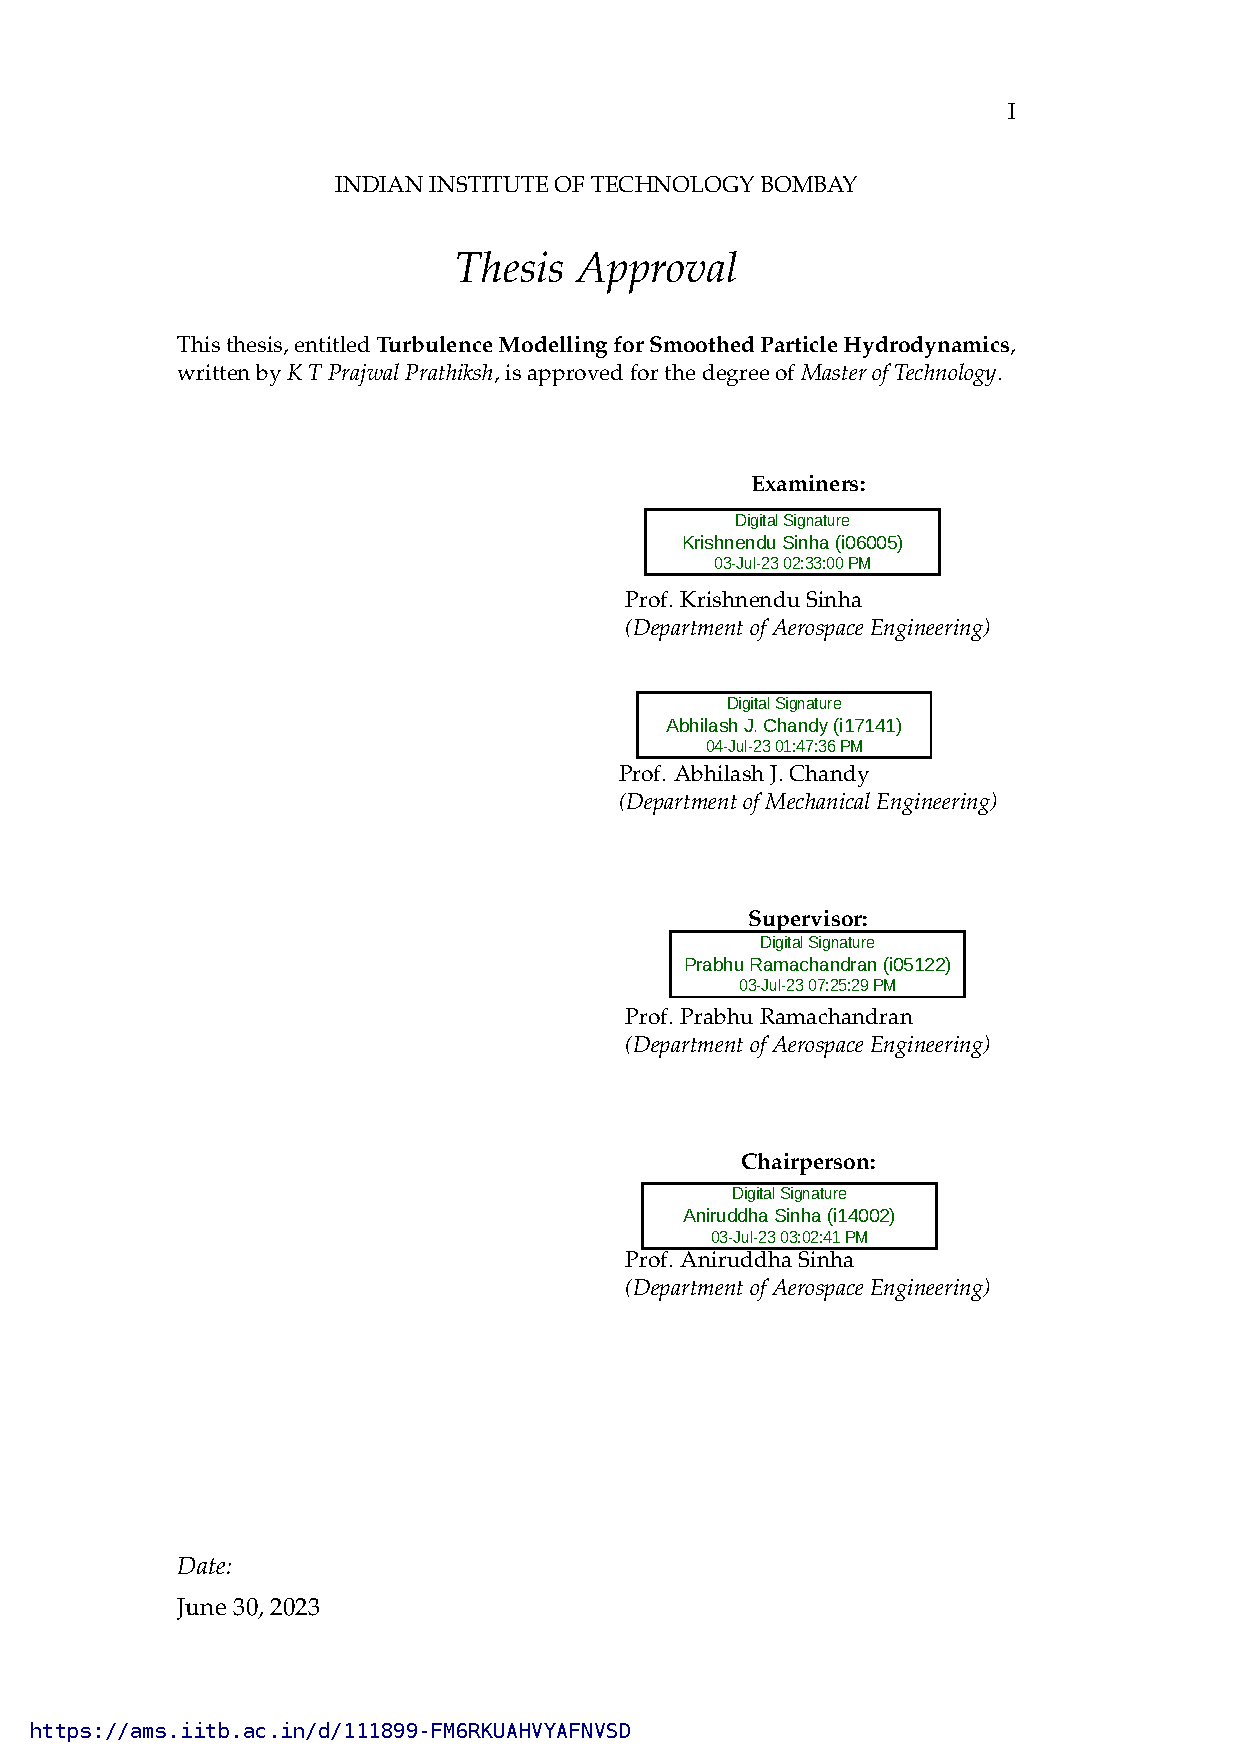
\includepdf[
  pages={1},
  pagecommand={\thispagestyle{plain}},
  addtotoc={1,chapter,1,Thesis Approval,thesis-approval}
]{Base/thesis-approval-180010027-signed.pdf}
% %----------------------------------------------------------------------------------------
%  THESIS APPROVAL PAGE
%----------------------------------------------------------------------------------------
\begin{center}
    {\normalsize \MakeUppercase{\univname} \par}% University name in capitals
    \bigskip
    {\huge\textit{Thesis Approval} \par}
    \bigskip
\end{center}

This thesis, entitled \textbf{\ttitle}, written by \textit{\authorname}, is approved for the degree of \textit{\degreename}.

\begin{minipage}[t]{\textwidth}
    \raggedleft
    \vspace{0.5cm}    
    {
        \renewcommand{\arraystretch}{2}%
        \centering
        \begin{tabular}{c}
            \textbf{Examiners:} \\ [0.5cm]
            
            \vtop{\hbox{\strut Prof. Krishnendu Sinha}\hbox{\strut \textit{(Department of Aerospace Engineering)}}}\\ [0.75cm]

            \vtop{\hbox{\strut Prof. Abhilash J.Chandy}\hbox{\strut \textit{(Department of Mechanical Engineering)}}}\\ [1.5cm]

            \textbf{Supervisor:} \\ [0.5cm]

            \vtop{\hbox{\strut Prof. Prabhu Ramachandran}\hbox{\strut \textit{(Department of Aerospace Engineering)}}}\\ [1.5cm]


            \textbf{Chairperson:} \\ [0.5cm]

            \vtop{\hbox{\strut Prof. Aniruddha Sinha}\hbox{\strut \textit{(Department of Aerospace Engineering)}}}\\ [0.75cm]
        \end{tabular}
    }
\end{minipage}

\vspace{0.2\textwidth}
\noindent \begin{minipage}[t]{0.5\textwidth}
    \begin{flushleft}
        \large
        \emph{Date:}\\ \vspace{0.03\textwidth}
        June 30, 2023
    \end{flushleft}
\end{minipage}


% Include declaration of independence
%----------------------------------------------------------------------------------------
%  DECLARATION PAGE (Declaration of Independence)
%----------------------------------------------------------------------------------------

\begin{declaration}
    \addchaptertocentry{\authorshipname} % Add the declaration to the table of contents
    
    \noindent I, \authorname, hereby declare that this written submission on \textit{\enquote{\ttitle}}, represents my ideas in my own words and where others' ideas or words have been included, I have adequately cited and referenced the original sources. I also declare that I have adhered to all principles of academic honesty and integrity and have not misrepresented or fabricated or falsified any idea/data/fact/source in my submission. I understand that any violation of the above will be cause for disciplinary action by the \emph{\univname}, and can also evoke penal action from the sources which have thus not been properly cited or from whom proper permission has not been taken when needed.


    \vspace{0.2\textwidth}
    \noindent \begin{minipage}[t]{0.5\textwidth}
        \begin{flushleft}
            \large
            \emph{Date:}\\ \vspace{0.03\textwidth}
            June 30, 2023% \today
        \end{flushleft}
    \end{minipage}
    \begin{minipage}[t]{0.5\textwidth}
        \begin{flushright}
            \large
            \emph{Student Name:} \authorname\\ \vspace{0.03\textwidth}
            \emph{Roll No.:} \matnumber
        \end{flushright}
    \end{minipage}
\end{declaration}


\cleardoublepage

% Include quotation page
% %----------------------------------------------------------------------------------------
%  QUOTATION PAGE (For a deep quote about the topic)
%----------------------------------------------------------------------------------------

\vspace*{0.2\textheight}

\noindent\enquote{\itshape Programming today is a race between software engineers striving to build bigger and better idiot-proof programs, and the universe trying to build bigger and better idiots. So far, the universe is winning.}\bigbreak

\hfill Rick Cook

% Include abstract page
%----------------------------------------------------------------------------------------
%  ABSTRACT PAGE
%----------------------------------------------------------------------------------------
\MakeShortVerb{\|}

\begin{abstract}
    \addchaptertocentry{\abstractname} % Add the abstract to the table of contents
    Turbulence modelling is a challenging problem, particularly for a Lagrangian method such as Smoothed Particle Hydrodynamics (SPH) which lacks the years of theoretical and practical research that conventional CFD solvers based on FEM/FVM enjoy.
    However, work based on translating existing Eulerian-based turbulence methods to SPH and Lagrangian-specific models has started making inroads in the general understanding of the topic in an SPH setting. Ultimately, a rigorous and robust model can be devised, which is suitable for a wide variety of $2D$ and $3D$ problems.
    
    This project aims to survey and review the state-of-the-art turbulence models that SPH offers and help subsequently provide a comparative analysis detailing the advantages and limitations of these models.
    It also intends to extend the best-equipped models to robust and accurate SPH schemes and incorporate some of the latest developments in the field of SPH to refine further the machinery required to model turbulence.
    
    \medskip
    \noindent \textbf{Keywords:} \keywordnames
\end{abstract}

% Include acknowledgements page
%----------------------------------------------------------------------------------------
%  ACKNOWLEDGEMENTS
%----------------------------------------------------------------------------------------

\begin{acknowledgements}
  \addchaptertocentry{\acknowledgementname}

  I would like to express my deepest gratitude and appreciation for \supname, my supervisor, for his invaluable guidance and support throughout the process of completing my academic thesis. His expertise, commitment, and insightful feedback have been instrumental in shaping this work and have significantly contributed to my growth as a researcher. His encouragement and patience, particularly during challenging times, have been a source of inspiration and motivation.
  It proved, indeed, to be a privilege to work under his supervision.
  
  I would also like to sincerely appreciate the academic environment and resources provided by \emph{\univname}. The stimulating scholarly community, state-of-the-art facilities, and access to extensive research materials have played an indispensable role in shaping my research journey.
  
  I would like to thank the \emph{\deptname} for providing me with the opportunity to pursue my graduate studies. The input and feedback provided by the faculty members have been invaluable in helping me develop my research skills.
  I must also acknowledge the facilities and resources provided by the \emph{\deptname}, particularly the \href{https://varuna.aero.iitb.ac.in/ace/}{\emph{Aerospace Computational Engine - ACE}} HPC cluster, which has been crucial to the completion of this work.
  
  I would also like to thank the members of the lab group headed by \supname for their support and guidance. Amal S Sebastian, Abhinav Muta, Asmelash Haftu, Pawan Negi, and Navaneet \textit{(in no particular order)} helped provide an environment conducive to learning and growth. I must acknowledge their generous sharing of knowledge and encouragement.
  Their contributions have enriched my research experience and have made this journey more enjoyable.
  
  Lastly, I extend my heartfelt gratitude to my family and friends for their unwavering support, understanding, and patience throughout this academic pursuit. Their unconditional love and encouragement have been my source of strength and motivation.

\end{acknowledgements}


%----------------------------------------------------------------------------------------
%  LIST OF CONTENTS/FIGURES/TABLES PAGES
%----------------------------------------------------------------------------------------

{\hypersetup{linkcolor=black} % Black links in all lists
  \tableofcontents % Prints the main table of contents
  \listoffigures % Prints the list of figures
  % Chapter* List of Symbols

\chapter*{List of Symbols} % Main chapter title
\addcontentsline{toc}{chapter}{List of Symbols}

\label{chap:list-of-symbols}

\setlength{\tabcolsep}{10pt} % Default value: 6pt - Column Spacing
\renewcommand{\arraystretch}{1.7} % Default value: 1 - Row Spacing

\begin{longtable}{ll}
\textbf{Symbol}         & \textbf{Description}              \\
\endfirsthead
%
\multicolumn{2}{c}%
{{\bfseries Table \thetable\ continued from previous page}} \\
\textbf{Symbol}         & \textbf{Description}              \\
\endhead
%
$\vect{a}$              & Vector Field                      \\
$\tensor{A}$            & Second-rank Tensor Field          \\
$\BasisVect$            & $i^{th}$ Basis                    \\
$\otimes$               & Tensor Product                    \\
$\LagDerivative{()}$    & Lagrangian Derivative             \\
$\FrobeniusInnerProduct{A}{B}$ & Frobenius Inner Product of $\tensor{A}$ and $\tensor{B}$                                    \\
$\FrobeniusNorm{A}$            & Frobenius Norm of $\tensor{A}$ $( = \sqrt{\FrobeniusInnerProduct{A}{A}})$ \\
$\nabla^2$              & Laplacian Operator                \\
$\Delta ()$             & Component-wise Laplacian Operator \\
$(1 - \alpha^2 \Delta)$ & Helmholtz Operator                \\
$i$                     & Reference Particle                \\
$j$                     & Neighbouring Particle             \\
$(...)_{i}$             & Property of $i^{th}$ SPH particle \\
$(...)_{j}$             & Property of $j^{th}$ SPH particle \\
$(...)_{ij}$            & $(...)_{i} - (...)_{j}$           \\
$t$                     & Time                              \\
$\vect{r}$              & Position $=(x, y, z)$             \\
$\vect{v}$              & Velocity $=(v_x, v_y, v_z)$       \\
$m$                     & Mass                              \\
$P$                     & Pressure                          \\
$\rho$                  & Density                           \\
$(...)_0$                      & Initial Condition ($(t=0$ of Specified Property                                             \\
$\Delta t$              & Time Step                         \\
$\Delta x$              & Inter Particle Spacing            \\
$\delta (x)$            & Dirac Delta Function              \\
$W_{h}$                 & SPH Interpolating Kernel          \\
$h$                     & Kernel Smoothing Length           \\
$\WIJ$                  & $W(|\RIJ|, h)$                    \\
$\DWIJ$                        & $\nabla_i W(\RIJ,h) = \frac{\RIJ}{\RtwoIJ[]} \PartialDerivative[r_i]{\WIJ}$                 \\
$\Vol_i$                & Volume of $i^{th}$ SPH particle   \\
$\varphi_i$                    & Particle Density of $i^{th}$ SPH particle                                                   \\
$\vect{F}$              & External Body Force               \\
$\nu$                   & Kinematic Viscosity               \\
$\eta$                  & Dynamic Viscosity $(=\nu \rho)$   \\
$\MachineEpsilon$       & Machine Epsilon                   \\
$M_o$                   & Reference Mass                    \\
$P_o$                   & Reference Pressure                \\
$\rho_o$                & Reference Density                 \\
$c_s$                   & Speed of Sound                    \\
$\gamma$                & Exponent - Equation of State      \\
$\Vorticity$                   & Vorticity $(=\nabla \times \vect{v})$                                                       \\
$\nu_t$                 & Turbulent Eddy Viscosity          \\
$\tensor{S}$                   & Strain-Rate Tensor $(=[1/2][\nabla \vect{v} + \nabla \vect{v}^T])$                          \\
$\tensor{R}$                   & Rate of Rotation Tensor $(=[1/2][\nabla \vect{v} - \nabla \vect{v}^T])$                     \\
$\epsilon$              & Turbulent Dissipation Rate        \\
$k$                     & Turbulent Kinetic Energy          \\
$\tensor{\tau}$         & Stress Tensor                     \\
$C_s $                  & Smagorinsky Constant              \\
$u_{max}$               & Maximum Particle Velocity         \\
$\varepsilon$           & Smoothing Parameter (XSPH)        \\
$\WaveNumber$           & Wave Number                      
\end{longtable} % Prints the list of 
  \listoftables % Prints the list of tables
%   \lstlistoflistings % Prints the list of (code) listings
%   \addchaptertocentry{Listings} % Add the list of listings to the table of contents
}


%----------------------------------------------------------------------------------------
%  ABBREVIATIONS
%----------------------------------------------------------------------------------------
  
% \chapter{\abbrevname}
% \begin{acronym}[AAAAAA]
%   \acro{acl}[ACL]{Access Control List}
%   \acro{ajax}[AJAX]{Asynchronous JavaScript and XML}
%   \acro{api}[API]{Application Programming Interface}
%   \acro{css}[CSS]{Cascading Style Sheets}
%   \acro{gui}[GUI]{Graphical User Interface}
%   \acro{html}[HTML]{Hypertext Markup Language}
%   \acro{json}[JSON]{JavaScript Object Notation}
%   \acro{php}[PHP]{PHP Hypertext Preprocessor}
%   \acro{sql}[SQL]{Structured Query Language}
%   \acro{uid}[UID]{User Identifier}
%   \acro{url}[URL]{Uniform Resource Locator}
%   \acro{ux}[UX]{User Experience}
%   % \acro{}[]{}
% \end{acronym}
% Use 
% - \ac{id} for standard behavior (\Ac{id} for first letter capitalized)
% - \acs{id} for acronym
% - \acl{id} for long version
% - \acp{id} for plural (with 's' at the end)
% - \acf{id} for the full version (long name + acronym in parentheses)
% - \newacro{id}[Acronym]{Long Name} to define acronyms outside the abbreviations list; e.g. for shorthands
% See https://ctan.mirror.norbert-ruehl.de/macros/latex/contrib/acronym/acronym.pdf

% \newpage


% ------ GLOSSARY ------

% \chapter{\glossaryname}

\begin{longtable}{p{5cm}p{10cm}}
    \textbf{Concept} & \textbf{Explanation} \\
    \hline
    \\
    \textbf{Access Control List (ACL)} & An Access Control List is a functionality that controls access to data for specific users via permissions.\\
    \\
    \textbf{Application Programming Interface (API)} & An Application Programming Interface is an interface that can be used in software development to access functions of other systems.\\
    \\
    \textbf{Backend} & The backend is the part of an application or system with which a user does not interact directly, and which performs actions in the background. A user interacts indirectly with the backend via the frontend.\\
    \\
    \textbf{Frontend} & A frontend is the part of an application or system that a user accesses directly. This is sometimes used as a synonym for the user interface of an application.
\end{longtable}



%----------------------------------------------------------------------------------------
%  THESIS CONTENT - CHAPTERS
%----------------------------------------------------------------------------------------

\mainmatter % Begin numeric (1,2,3...) page numbering

\pagestyle{thesis} % Return the page headers back to the "thesis" style

% Include the chapters of the thesis as separate files from the Chapters folder
% Uncomment the lines as you write the chapters

% Chapter 1

\chapter{Introduction}
\label{chap:introduction}


\epigraph{Turbulence is the most important unsolved problem of classical physics.}{\textit{Richard Feynman}}

Turbulent flows have long been a phenomenon that is surprisingly easy to detect and observe in the natural world but unmistakably challenging to understand and model in sufficient detail, unlike other problems in classical physics.
The fundamental aspects of turbulent flow consisting of eddies of various length scales had long been observed, as reflected in the $16^{th}$ century diagrams by Leonardo Da Vinci consisting of water flow in streams and channels.
It took the work of Osborne Reynolds on his averaging of the Navier-Stokes (NS) equations and William Thomson's (Lord Kelvin) work on flow along an inclined plane (see \figref{fig:schmitt2017turbulence-fig-1}) for \textit{turbulence} to enter the parlance of the larger scientific community. This allowed turbulence to be recognised as a new subfield of fluid mechanics.

However, further strides in the field have remained arduous despite the Navier-Stokes equations being written down in the early $19^{th}$ century. There is consensus that this remarkable failure of some of the greatest scientific minds in providing an intricate understanding of turbulence points to an inadequacy of the mathematical tools we have at our disposal. Even the current machinery cannot deal with the strong non-linearity of the equations coupled with the characteristic tendency of flows to degenerate into some form of instability.

\begin{figure}[htbp!]
    \centering
    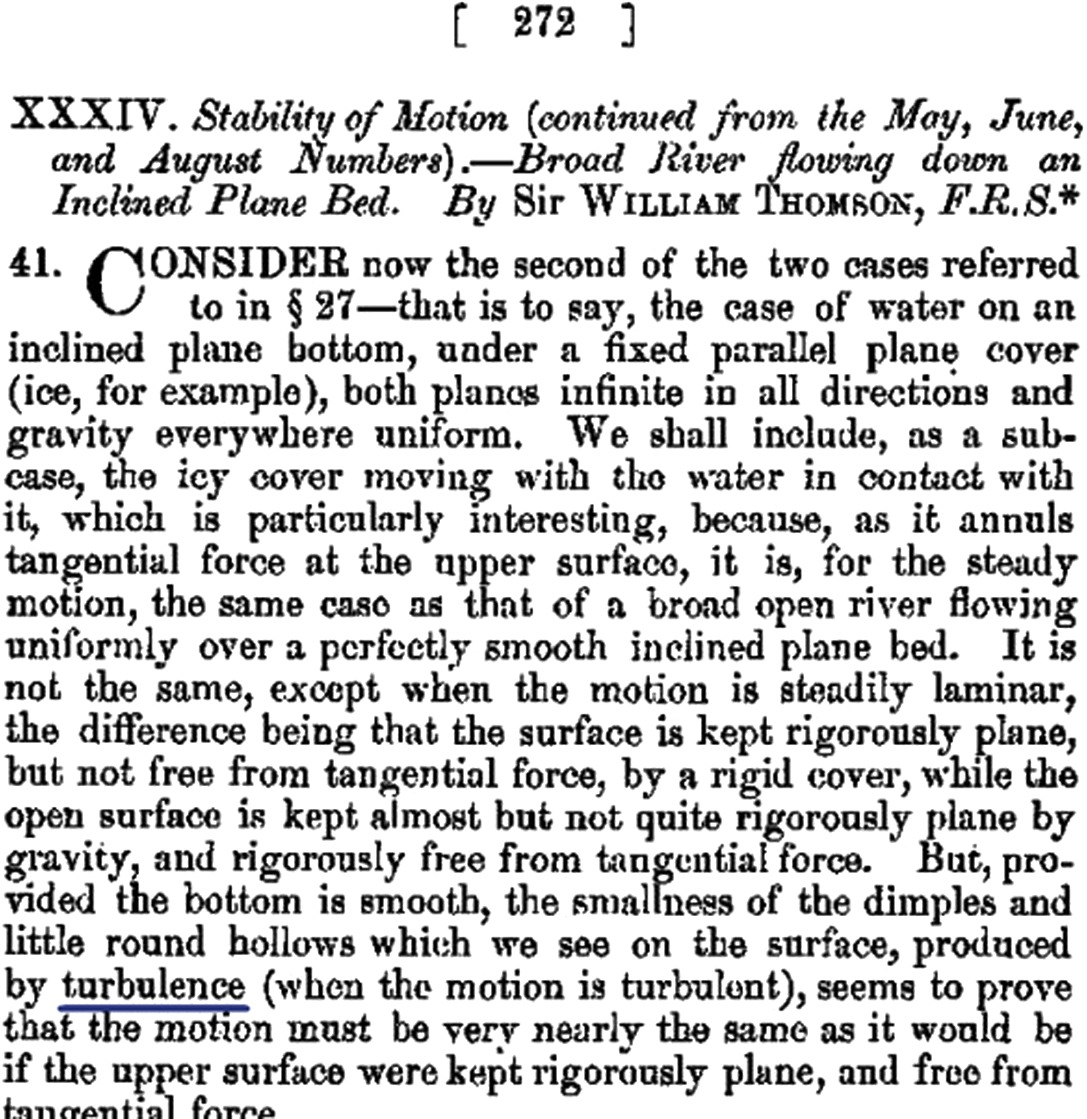
\includegraphics{Figures/research_papers/schmitt2017turbulence-fig-1.jpg}
    \caption{A scanned copy of a part of the first page of the 1887 paper by William Thomson, where the word \textit{'turbulence'}, as a noun, is first introduced. Reproduced from \cite{schmitt2017turbulence}}
    \label{fig:schmitt2017turbulence-fig-1}
\end{figure}

Turbulence is caused by excessive kinetic energy in parts of a fluid flow that can overcome the damping effect of the fluid's viscosity. Its onset can be predicted by the dimensionless Reynolds number, which is the ratio of kinetic energy to viscous damping in a fluid flow. 

The criteria for defining a flow as turbulent are varied and ambiguous since there is no explicit definition for it. However, the most often used criteria for qualifying a flow as turbulent is given below \parencite{sagaut2002statistical}:
\begin{itemize}
    \item random character of the spatial and temporal fluctuations of the velocities, which reflect the existence of finite characteristic scales of statistical correlation;
    \item velocity field is three-dimensional and rotational;
    \item various modes are strongly coupled, which is reflected in the non-linearity of the NS equations;
    \item large mixing capacity due to the agitation induced by the various scales;
    \item chaotic character of the solution, which exhibits a powerful dependency on the initial condition and boundary conditions.
\end{itemize}

%----------------------------------------------------------------------------------------
%	Section 1 - Smoothed Particle Hydrodynamics
%----------------------------------------------------------------------------------------
\section{Smoothed Particle Hydrodynamics}
Smoothed particle hydrodynamics (SPH) is a technique for problem-solving in \textit{Computational Continuum Dynamics} (CCD). This technique approximates numerical solutions of the equations of fluid dynamics by replacing the fluid with a set of particles. The equations of motion and properties of these particles are determined from the continuum equations of fluid dynamics. They are subsequently discretised based on the particles' interpolant data. The interpolant can be constructed using analytical functions, and spatial derivatives of the interpolated quantities can then be found using ordinary calculus. There is no need to use a grid, and the description of free surfaces, however complicated, is trivial.

Therefore, this \textit{Lagrangian} based particle formulation uses no background spatial mesh. Since there is no mesh to distort, the method can handle large deformations in a pure Lagrangian frame. Thus, material interfaces can be modelled naturally, and complex constitutive behaviour can be implemented relatively quickly. This allows SPH to have diverse and fascinating applications in various domains that extend beyond the astrophysical and cosmological problems it was initially designed to tackle.

%----------------------------------------------------------------------------------------
%	Section 2 - Project Motivation \& Objectives
%----------------------------------------------------------------------------------------
\section{Project Motivation \& Objectives}
Despite the success of SPH in simulating transient flows, a robust or rigorous model of turbulence does not seem to exist. Some of the models in use cannot be generalised to a wide variety of turbulence-based problems or scaled to $3D$-flows.
This limits SPH's applicability in turbulent flows where conventional FEM/FVM-based CFD solvers have the upper hand, owing to their sophisticated models.

This project aims to survey and review the current state of the art regarding turbulence modelling in SPH and subsequently provide a framework to help establish the advantages and limitations of such models, using a comparative analysis between the major class of models.
After that, it is intended to extend the most well-equipped models to robust and accurate SPH schemes (which might not have been the case in the author/s original work) for bounded flows specifically. Such an exercise is expected to either improve the original model or expose any underlying limitations in its assumptions or discretisation.

%----------------------------------------------------------------------------------------
%	Section 3 - Large Eddy Simulation-based Models
%----------------------------------------------------------------------------------------
\section{Report Structure}
The report is structured to present the turbulence models developed for SPH in \chapref{chap:turbulence-modelling}. Here, the models have been categorised by the fundamental ideas on which they were based. In \chapref{chap:evaluation-of-turbulence-models}, research on analysing turbulence through standard benchmarks problems and methods of quantifying turbulence data is presented.
Subsequently, the implementation of the models, and their results are presented in \chapref{chap:results}.
Finally, the project conclusion and future work are presented in \chapref{chap:conclusions-and-future-work}.

% Chapter 2

\chapter{Turbulence Modelling} % Main chapter title

\label{chap:turbulence-modelling}
%----------------------------------------------------------------------------------------
%	Section 1 - Viscosity-Based Models
%----------------------------------------------------------------------------------------
\section{Viscosity-based Models}
\label{sec:visc-based-model}
\cite{VIOLEAU2002} were amongst the early pioneers who tried to incorporate a turbulence model in SPH. They came up with two techniques to tackle the problem of turbulence in a Lagrangian framework, which so far had been neglected till then in research, namely, the eddy viscosity model and a generalised Langevin model. For each of their techniques, they considered the following equation of state \Eqref{eq:violeau-eos}, continuity equation \Eqref{eq:violeau-continuity} and momentum equation \Eqref{eq:violeau-mom}, based on the work of \cite{Monaghan1992}:   
\begin{equation}
    P_i = B \Bigg[ \bigg( \frac{\rho_i}{\rho_o} \bigg)^{\gamma} - 1 \Bigg] \quad , \quad B = \frac{\rho_o c_s^2}{\gamma}
    \label{eq:violeau-eos}
\end{equation}
Where, $(P, \rho)$ denotes pressure and density respectively. $(...)_i$ denotes the property of the $i^{th}$ SPH particle, $(...)_o$ denotes the reference quantities, and $(c_s)$ denotes the speed of sound.
\begin{equation}
    \LagDerivative{\rho_i} = \sum_j m_j \VIJ \cdot \DWIJ
    \label{eq:violeau-continuity}
\end{equation}
Where $[\LagDerivative{()}]$ denotes the Lagrangian derivative, and $(m, \vect{v})$ represent the mass and velocity respectively. Here we adopt the nomenclature of $(...)_{ij}$ to denote the difference of a specified property between the $i^{th}$ and $j^{th}$ SPH particle $[(...)_{i} - (...)_{j}]$, and $(\DWIJ)$ denotes $[\nabla_i W(\RIJ,h) = \frac{\RIJ}{\RtwoIJ[]} \PartialDerivative[r_i]{\WIJ}]$, where $(h)$ is the kernel smoothing length.
\begin{equation}
    \LagDerivative{\vect{v}_i} = - \sum_j m_j \bigg( \frac{P_i}{\rho_i^2} + \frac{P_j}{\rho_j^2} + \Pi_{ij} \bigg) \DWIJ + \vect{F}_i
    \label{eq:violeau-mom}
\end{equation}
Where $(\vect{F})$ is the external body force, and the viscous term $(\Pi)$ is defined as:
\begin{equation}
    \Pi_{ij} = - \frac{16\nu}{\rho_i + \rho_j} \frac{\VIJ \cdot \RIJ}{\RtwoIJ + \MachineEpsilon^2} 
    \label{eq:violeau-diffusion-term}
\end{equation}
Here $(\nu)$ is the kinematic viscosity, and $(\MachineEpsilon)$ is the machine epsilon.


\subsection{Eddy Viscosity Model}
\label{sec:eddy-visc-model}
The eddy viscosity model was devised as a first-order closure model, which consisted of a relationship between the Reynolds stress tensor and the mean velocity gradients. Therefore, the momentum equation is similar to the equation in \Eqref{eq:violeau-mom}, except that the kinematic viscosity is replaced by the eddy viscosity $(\nu_t)$, and the velocities are Reynolds-averaged. In the SPH formalism, the diffusion term occurring is therefore defined as given in \Eqref{eq:violeau-turbulent-diffusion-term}, with the eddy viscosity defined according to \Eqref{eq:violeau-eddy-viscosity}.
\begin{equation}
    \widetilde{\Pi}_{ij} = -8 \frac{\nu_{t, i} + \nu_{t, j}}{\rho_i + \rho_j} \frac{\RAProp{\vect{v}}_{ij} \cdot \RIJ }{\RtwoIJ + \MachineEpsilon^2}
    \label{eq:violeau-turbulent-diffusion-term}
\end{equation}
\begin{equation}
    \nu_t = L_m^2 \FrobeniusNorm{S} = L_m^2 \sqrt{\FrobeniusInnerProduct{S}{S}}
    \label{eq:violeau-eddy-viscosity}
\end{equation}
Where $\RAProp{\vect{v}}$ is Reynolds-averaged velocity, $L_m$ refers to the mixing length scales, and $(\tensor{S})$ is the strain-rate tensor $(=[1/2][\nabla \vect{v} + \nabla \vect{v}^T])$, where we adopt the nomenclature of $(\tensor{A})$ to represent a second-rank tensor field. Also, here $(\FrobeniusInnerProduct{A}{B})$ denotes the Frobenius inner product of $\tensor{A}$ and $\tensor{B}$, and $(\FrobeniusNorm{A})$ denotes the Frobenius norm of $\tensor{A}$ $( = \sqrt{\FrobeniusInnerProduct{A}{A}})$.
The SPH formulation for the mean velocity gradients are given in \Eqref{eq:violeau-mean-velocity-gradient}.
\begin{equation}
    \nabla \RAProp{\vect{v}}_i = - \frac{1}{\rho_i} \sum_j m_j \RAProp{\vect{v}}_{ij} \otimes \DWIJ
    \label{eq:violeau-mean-velocity-gradient}
\end{equation}
Where $(\otimes)$ denotes the tensor product.

On simulating Poiseuille flow for a high Reynolds number case, the authors could show that the velocity profile showed only a slight discrepancy with theory, with the expected log-law profile near the walls \figref{fig:violeau2002-eddy-viscosity-result}. This indicated that the model is appropriate for turbulent mixing problems or for cases involving spatially-varying viscosity while restricted to shear flows.

\begin{figure}[H]
    \centering
    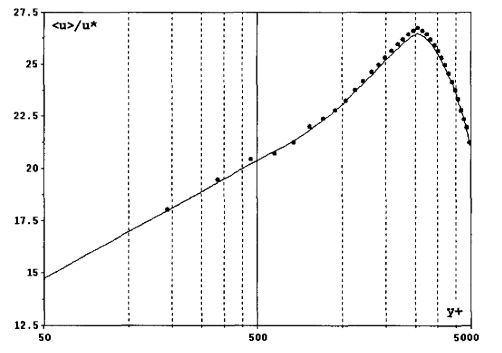
\includegraphics{Figures/research_papers/violeau2002-eddy-viscosity-result.png}
    \caption{Turbulent Poiseuille flow in a pipe $(Re = \SciNot{6.4}{4})$ modelled using the eddy viscosity model. Computed mean velocity profiles after $(t=1s)$ (solid circles), against theory (solid line). Reproduced from \cite{VIOLEAU2002}}
    \label{fig:violeau2002-eddy-viscosity-result}
\end{figure}

\subsection{Generalized Langevin Model}
\cite{VIOLEAU2002} also considered a stochastic approach, where the main idea is built on the concept of prescribing particle velocities as a random process, with properties fulfilling the theoretical turbulence hypotheses \parencite{pope1994lagrangi}. Hence, came about the Generalised Langevin model (GLM), where the particle acceleration is defined as:
\begin{equation}
    d\vect{v} = -\frac{1}{\rho} \nabla \RAProp{P} + \tensor{G}(\vect{v} - \RAProp{\vect{v}})dt + \sqrt{C_0 \epsilon dt}\Vec{\xi}
    \label{eq:violeau-glm-particle-accel}
\end{equation}
Where $\Vec{\xi}$ is a random vector statistically non-correlated with velocities. The closure for this model was defined by specifying $\tensor{G}$ as:
\begin{equation}
    \tensor{G} = \HalfFrac C_1 \frac{\epsilon}{k}\tensor{I} + C_2 \nabla \RAProp{\vect{v}}
\end{equation}
Where $(k)$ is the turbulent kinetic energy, $(\epsilon)$ the dissipation rate, and $(C_i)$ being constants - $(C_1=1.8, C_2=0.6)$. $(\tensor{I})$, here, denotes the identity tensor.
By modelling turbulence as GLM in SPH, the momentum equation derived was given by:
\begin{equation}
    \LagDerivative{\vect{v}_i} = -\sum_j m_j \bigg( \frac{\RAProp{P}_i}{\rho_i^2} + \frac{\RAProp{P}_j}{\rho_j^2} \bigg) \DWIJ - \HalfFrac C_1 \frac{\epsilon_i}{k_i} \vect{v}'_i + C_2 \nabla \RAProp{\vect{v}}_i \cdot \vect{v}'_i + \sqrt{\frac{C_0 \epsilon_i}{\Delta t}} \Vec{\xi}_i
    \label{eq:violeau-mom-glm}
\end{equation}
\begin{equation}
    \RAProp{\vect{v}} = \sum_j \frac{m_j}{\rho_j}\vect{v}_j W_h (\vect{r}_j)
    \label{eq:violeau-ra-vel}
\end{equation}
Where the fluctuations are defined as $\vect{v}' = \vect{v} - \RAProp{\vect{v}}$, and the local values of turbulent kinetic energy and dissipation rate are:
\begin{align}
    \epsilon_i = 2 \nu_{t, i} + 
    \FrobeniusNorm{S_i}^2 \\
    k_i = \frac{\epsilon_i \nu_{t, i}}{C_{\mu}} \quad , \quad C_{\mu} = 0.009
    \label{eq:violeau-k-eps}
\end{align}

It is to be noted that the authors did not estimate the dissipation rate through the proper velocity gradients since the fluctuations of random velocities do not reproduce the small eddies.
The same test case as mentioned in \secref{sec:eddy-visc-model} was considered for the performance of GLM. 
The authors observed large fluctuations. They attributed the discrepancy to the mean operator being redefined as given by \Eqref{eq:violeau-ra-vel} instead of being a Reynolds average. In fact, by redefining the mean operator in such a fashion, they appeared to have constructed a rudimentary LES filter. 
As observed in \figref{fig:violeau2002-GLM-result}, the fluctuations have an order of magnitude of $k^{1/2}$. However, as claimed by the authors, unlike the eddy viscosity model, the GLM method can be used for different flows instead of being restricted to only shear flows.
\begin{figure}[H]
    \centering
    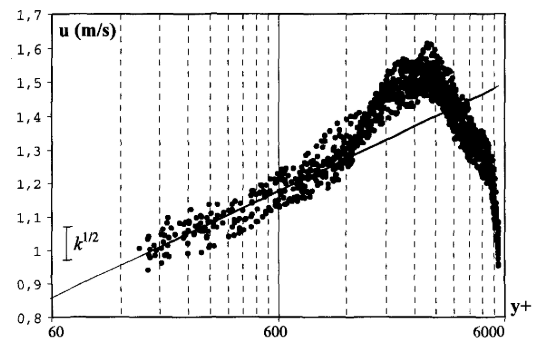
\includegraphics{Figures/research_papers/violeau2002-GLM-result.png}
    \caption{Turbulent Poiseuille flow in a pipe $(Re = \SciNot{6.4}{4})$ modelled using the generalised Langevin model. Computed mean velocity profiles after $(t=1s)$ (solid circles), against theory (solid line). Reproduced from \cite{VIOLEAU2002}}
    \label{fig:violeau2002-GLM-result}
\end{figure}


\subsection{mSPH}
\cite{Adami2012} devised a model built on their observation of SPH simulations, wherein the absence of viscosity in typical SPH formulations produced purely noisy particle motion. At finite viscosities, the method would over-predict dissipation. Hence to counter this, they essentially ``modified'' (hence the name: Modified SPH [mSPH]) the momentum equation and the equation of state to advect the particles in order to homogenise the particle distribution, in turn stabilising the numerical scheme. They were also able to reduce the artificial dissipation in transitional flows.

The authors considered summation density (\Eqref{eq:Adami2012-summation-density}), which is a function of the volume of the respective SPH particle as given by \Eqref{eq:Adami2012-vol}, as opposed to evolving density through the continuity equation \parencite{hu2006multi}. The modified equation of state as given by \Eqref{eq:Adami2012-eos}, is equivalent to the classical SPH equation-of-state with $\gamma=1$.
\begin{equation}
    \Vol_i = \frac{1}{\sum_j \WIJ}
    \label{eq:Adami2012-vol}
\end{equation}
\begin{equation}
    \rho_i = \frac{m_i}{\Vol_i} = m_i\sum_j \WIJ
    \label{eq:Adami2012-summation-density}
\end{equation}
\begin{equation}
    P_i = c_s^2 (\rho_i - \rho_o)
    \label{eq:Adami2012-eos}
\end{equation}
Where $(\Vol)$ represents the volume of a particle.

The momentum equation, which provides the acceleration of the particle, is a function of just the gradient and viscous shear forces as given by \Eqref{eq:Adami2012-mom-governing}. The corresponding SPH formulation was derived as given by \Eqref{eq:Adami2012-mom-sph}, which built on the earlier work of \cite{hu2007incompressible}.
\begin{equation}
    \LagDerivative{\vect{v}} = -\frac{1}{\rho}\nabla P + \nu \Delta( \vect{v} ) + \vect{F}
    \label{eq:Adami2012-mom-governing}
\end{equation}
\begin{equation}
    \LagDerivative{\vect{v}_i} = -\frac{1}{m_i} \sum_j (\Vol^2_i + \Vol^2_j) \frac{P_i \rho_j + P_j \rho_i}{\rho_i + \rho_i} \DWIJ - \frac{\eta}{m_i} \sum_j (\Vol^2_i + \Vol^2_j) \frac{\VIJ}{\RtwoIJ[]}\DWIJ + \vect{F}_i
    \label{eq:Adami2012-mom-sph}
\end{equation}
Where $[\Delta ()]$ denotes the component-wise Laplacian operator, and $(\eta)$ is the dynamic viscosity.

This scheme takes advantage of the regularisation of the
particle motion stemming from the additional background pressure $(P_o = \rho_o c_s^2)$. The additional force exerted by the background pressure counteracts non-homogeneous particle distributions, therein reducing numerical dissipation.

The authors estimated the energy spectra of the flow simulations in order to analyse the results of their test cases, using first and second-order moving-least-squares (MLS) method \parencite{gossler2001moving} and its subsequent Fourier transform \parencite{frigo2005design}.
Their first test case, the $2D$ variant of the Taylor-Green Vortex (TGV) problem, involved $8\times 8$ counter-rotating vortices, requiring $64^2$ particles. They considered the viscosity to be zero.
As seen in the time evolution of the 
\begin{figure}[H]
    \centering
    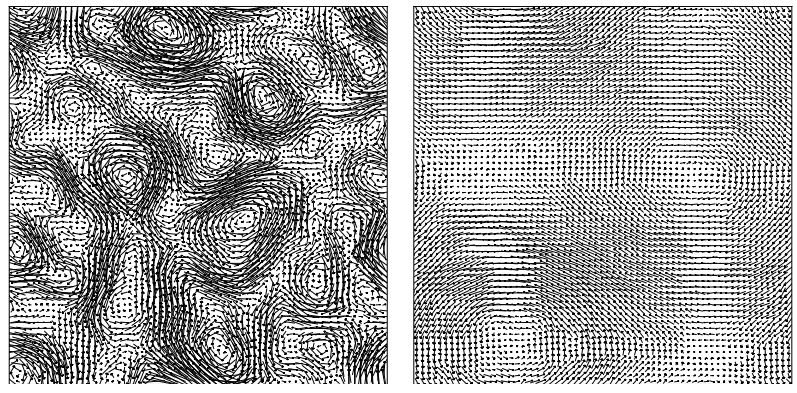
\includegraphics[scale=0.7]{Figures/research_papers/adami2012-evolution-vel-field-tgv.png}
    \caption{Velocity vector plot at $t=2$ (left) and $t=30$ (right). $Re = \infty$. Reproduced from \cite{Adami2012} }
    \label{fig:adami2012-evolution-vel-field-tgv}
\end{figure}

The time evolution of the velocity field is given in \figref{fig:adami2012-evolution-vel-field-tgv}, where it can be observed that the $2D$ turbulence is characterised by merging and pairing of small vortices. The energy spectra given in \figref{fig:adami2012-energy-spectra-tgv} show that at low wave numbers, both interpolation schemes give the same results, but at high wave numbers, the results differ. The energy spectrum of the standard SPH has a linear slope of magnitude $m = 1$ in a log-log scale equivalent to a purely noisy velocity field. Theoretically, however, $2D$ turbulence has an energy cascade with a slope of $m = -3$ in the inertial range, which is reasonably predicted using mSPH.
\begin{figure}[H]
    \centering
    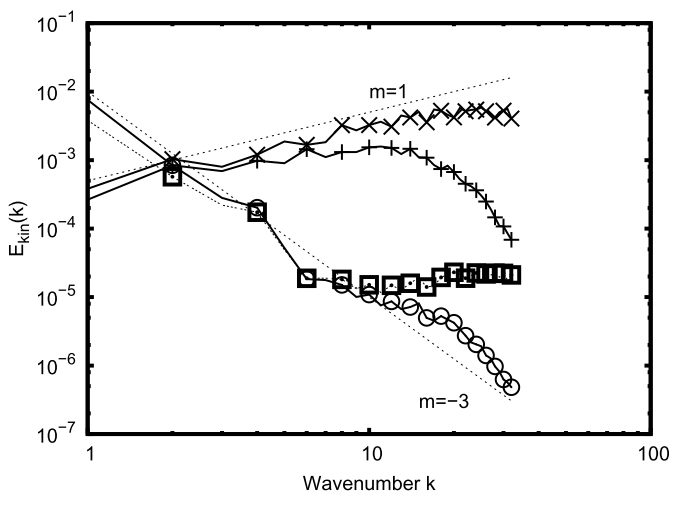
\includegraphics[scale=0.55]{Figures/research_papers/adami2012-energy-spectra-tgv.png}
    \caption{Comparison of energy spectra $t=10$. $+$ and $\times$ denote standard SPH results with quintic spline and MLS interpolation; $\circ$ and $\square$ denote mSPH results with quintic spline and MLS interpolation. Reproduced from \cite{Adami2012} }
    \label{fig:adami2012-energy-spectra-tgv}
\end{figure}

The second test case employed by the authors was that of the $3D$ TGV problem requiring $64^3$ particles for a wide range of Reynolds numbers. The dissipation rate of the flow simulations are shown in \figref{fig:adami2012-dissipation-re400} and \figref{fig:adami2012-dissipation-re3000}. It can be observed that the standard SPH is unable to simulate transitional flows due to excessive dissipation. In contrast, mSPH can reproduce the dissipation rate reasonably well. This implies that the corrected particle transport velocity is an analogous eddy-viscosity model on scales below the numerical resolution.
\begin{figure}[H]
    \centering
    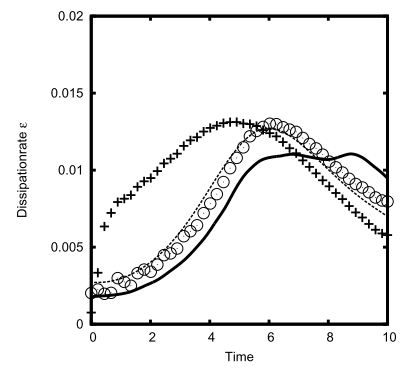
\includegraphics[scale=0.7]{Figures/research_papers/adami2012-dissipation-re400.png}
    \caption{Dissipation rate at $Re = 400$ using DNS (solid line), Smagorinsky model (dashed line), standard SPH ($+$) and mSPH ($\circ$). Reproduced from \cite{Adami2012}}
    \label{fig:adami2012-dissipation-re400}
\end{figure}
\begin{figure}[H]
    \centering
    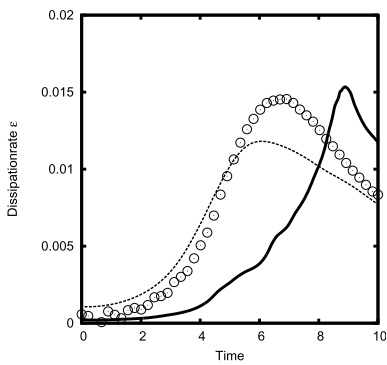
\includegraphics[scale=0.7]{Figures/research_papers/adami2012-dissipation-re3000.png}
    \caption{Dissipation rate at $Re = 3000$ using DNS (solid line), Smagorinsky model (dashed line) and mSPH ($\circ$). Reproduced from \cite{Adami2012}}
    \label{fig:adami2012-dissipation-re3000}
\end{figure}

%----------------------------------------------------------------------------------------
%	Section 2 - Large Eddy Simulation-based Models
%----------------------------------------------------------------------------------------
\section{Large Eddy Simulation-based Models}
\label{sec:les-based-model}
\subsection{Implicit Pressure Poisson-based Models}
\label{sec:Implicit-Pressure-Poisson-based-Models}
\cite{Gotoh2004} were amongst the first to integrate Large Eddy Simulation techniques with the SPH method. They derived this LES-SPH model, based on incompressible flow, to tackle the problem of reflection and transmission characteristics of regular waves by a partially immersed curtain-type breakwater. In order to compare the dissipation efficiencies, they considered the non-overtopping and overtopping cases of the problem.

The governing equations of the system were described as given by the continuity equation in \Eqref{eq:Gotoh2004-continuity-governing} and the momentum equation in \Eqref{eq:Adami2012-mom-governing}.
\begin{equation}
    \frac{1}{\rho} \LagDerivative{\rho} + \nabla \cdot \vect{v} = 0
    \label{eq:Gotoh2004-continuity-governing}
\end{equation}

The LES mass and momentum conservation equations for the flow were derived by filtering the respective equations using a spatial filter $\overline{(...)}$ to obtain their filtered counterparts as given by \Eqref{eq:Gotoh2004-continuity-filtered} and \Eqref{eq:Gotoh2004-mom-filtered} respectively.
\begin{equation}
    \frac{1}{\rho} \LagDerivative{\rho} + \nabla \cdot \vect{\overline{v}} = 0
    \label{eq:Gotoh2004-continuity-filtered}
\end{equation}
\begin{equation}
    \LagDerivative{\vect{\overline{v}}} = -\frac{1}{\rho}\nabla \overline{P} + \nu \Delta ( \vect{\overline{v}} ) + \frac{1}{\rho}\nabla\cdot\tensor{\tau} + \vect{F}
    \label{eq:Gotoh2004-mom-filtered}
\end{equation}
\begin{equation}
    \frac{1}{\rho} \tensor{\tau} = \vect{\overline{v}} \otimes \vect{\overline{v}} - \overline{\vect{v} \otimes \vect{v}}
    \label{eq:Gotoh2004-stress-tensor}
\end{equation}

The stress tensor $(\tensor{\tau})$ defined in \Eqref{eq:Gotoh2004-stress-tensor} is closed using Boussinesq’s Hypothesis as defined in \Eqref{eq:Gotoh2004-boussinesq}.
\begin{equation}
    \frac{1}{\rho} \tensor{\tau} = 2\nu_t \tensor{S} - \frac{2}{3}k\tensor{I}
    \label{eq:Gotoh2004-boussinesq}
\end{equation}

The turbulent eddy viscosity is estimated using a modified Smagorinsky model as given in \Eqref{eq:Gotoh2004-eddy-visc}. This allows wall effects to be incorporated into the model, which the authors required to tackle the problem they were working on.
\begin{equation}
    \nu_t = \min(C_s \Delta x, \kappa d_{wall})^2 \sqrt{2 \FrobeniusInnerProduct{S}{S}}
    \label{eq:Gotoh2004-eddy-visc}
\end{equation}
\begin{equation}
    C_s=0.1 \quad , \quad \kappa=0.4
\end{equation}
Where $(C_s)$ is the Smagorinsky constant, $(\kappa)$ is the von Karman constant, $d_{wall}$ is the normal distance of the particle to the closest wall, and $(\Delta x)$ is the inter-particle spacing.

The first term in \Eqref{eq:Gotoh2004-eddy-visc} dominates the flow far away from the solid wall, thereby recovering the standard Smagorinsky model. However, the second term dominates for flow close to the wall; hence, the eddy viscosity is a function of the particle distance to the wall. This overcomes the disadvantage of the standard Smagorinsky being over-dissipative inside the laminar layer.

In order to solve the system of equations and evolve them in time, the authors employed the Predictive-Corrective time integrator, similar to the two-step projection method of \cite{chorin1968numerical}. The prediction stage is outlined by \Eqref{eq:Gotoh2004-predict-start} - \Eqref{eq:Gotoh2004-predict-end}, where $(\delta t)$ denotes the time step.
\begin{equation}
    \Delta \vect{v}_* = \bigg( \nu \Delta ( \vect{\overline{v}} ) + \frac{1}{\rho}\nabla\cdot\tensor{\tau} + \vect{F} \bigg) \Delta t
    \label{eq:Gotoh2004-predict-start}
\end{equation}
\begin{equation}
    \vect{v}_* = \vect{v}_t + \Delta \vect{v}_*
\end{equation}
\begin{equation}
    \vect{r}_* = \vect{r}_t + \vect{v}_* \Delta t
    \label{eq:Gotoh2004-predict-end}
\end{equation}

The correction stage is outlined by \Eqref{eq:Gotoh2004-correct-start} - \Eqref{eq:Gotoh2004-correct-end}. $(\overline{P})$ which is required to update the $(\vect{v}_{t+1})$ term is calculated implicitly from \Eqref{eq:Gotoh2004-correct-pressure-implicit}, which is based on the filtered continuity equation given by \Eqref{eq:Gotoh2004-continuity-filtered} and assuming incompressibility $\LagDerivative{\rho}=0$.
\begin{equation}
    \Delta \vect{v}_{**} = -\frac{1}{\rho} \nabla \overline{P}_{t+1} \Delta t
    \label{eq:Gotoh2004-correct-start}
\end{equation}
\begin{equation}
    \nabla \cdot \bigg( \frac{1}{\rho_*} \nabla \overline{P}_{t+1} \bigg) = \frac{\rho_o - \rho_*}{\rho_o \Delta t^2}
    \label{eq:Gotoh2004-correct-pressure-implicit}
\end{equation}
\begin{equation}
    \vect{v}_{t+1} = \vect{v}_* + \Delta \vect{v}_{**}
\end{equation}
\begin{equation}
    \vect{r}_{t+1} = \vect{r}_t + (\vect{v}_t + \vect{v}_{t+1})\frac{\Delta t}{2}
    \label{eq:Gotoh2004-correct-end}
\end{equation}

In order to solve the system of equations given by \Eqref{eq:Gotoh2004-predict-start} - \Eqref{eq:Gotoh2004-correct-end} in an SPH setting, the authors presented the following SPH formulation for the flow property. The fluid density is given using a simple summation density \Eqref{eq:Gotoh2004-summation-density}.
\begin{equation}
    \rho_i = \sum_j m_j\WIJ
    \label{eq:Gotoh2004-summation-density}
\end{equation}

The pressure gradient term is defined in \Eqref{eq:Gotoh2004-grad-p-sph} in a symmetric form.
\begin{equation}
    \bigg( \frac{1}{\rho} \nabla \overline{P} \bigg)_i = \sum_j m_j \bigg( \frac{\overline{P}_i}{\rho_i^2} + \frac{\overline{P}_j}{\rho_j^2} \bigg) \DWIJ
    \label{eq:Gotoh2004-grad-p-sph}
\end{equation}

The divergence of $\vect{v}$ is also defined symmetrically as given by \Eqref{eq:Gotoh2004-div-u-sph}.
\begin{equation}
    \nabla \cdot \vect{\overline{v}}_i = \rho_i \sum_j m_j \bigg(\frac{\vect{\overline{v}}_i}{\rho^2_i} + \frac{\vect{\overline{v}}_j}{\rho^2_j} \bigg) \cdot \DWIJ
    \label{eq:Gotoh2004-div-u-sph}
\end{equation}

The pressure Laplacian, defined in \Eqref{eq:Gotoh2004-p-laplacian-sph}, is formulated as a hybrid of a standard SPH first derivative with a finite difference approximation for the first derivative to aid particle pressure stability \parencite{cummins1999sph}.
\begin{equation}
    \nabla \cdot \bigg( \frac{1}{\rho} \nabla \overline{P} \bigg)_i = \sum_j m_j \frac{8}{(\rho_i + \rho_j)^2} \frac{\overline{P}_{ij} \RIJ \cdot \DWIJ }{\RtwoIJ}
    \label{eq:Gotoh2004-p-laplacian-sph}
\end{equation}

The divergence of the stress tensor is defined in \Eqref{eq:Gotoh2004-div-tau-sph}.
\begin{equation}
    \bigg( \frac{1}{\rho} \nabla \cdot \tensor{\tau} \bigg)_i = \sum_j m_j \Bigg( \frac{1}{\rho_i^2}\tensor{\tau_i} + \frac{1}{\rho_j^2}\tensor{\tau_j} \Bigg) \cdot \DWIJ
    \label{eq:Gotoh2004-div-tau-sph}
\end{equation}

Finally, the laminar stress term, consisting of the velocity Laplacian term, is defined as given by \Eqref{eq:Gotoh2004-vel-laplacian-sph}.
\begin{equation}
    \big(\nu \Delta(\vect{\overline{v}}) \big)_i = \sum_j m_j \frac{4(\eta_i + \eta_j)}{(\rho_i + \rho_j)^2}\frac{\vect{\overline{v}}_{ij} \RIJ \cdot \DWIJ}{\RtwoIJ}
    \label{eq:Gotoh2004-vel-laplacian-sph}
\end{equation}

The authors used this SPH-LES model to investigate the wave interaction with a partially immersed breakwater and compared the results with experimentally obtained values of a similar setup. Their computational domain was $2D$ populated by $\approx 1.2 \times  10^4$ particles.

\begin{figure}[H]
    \centering
    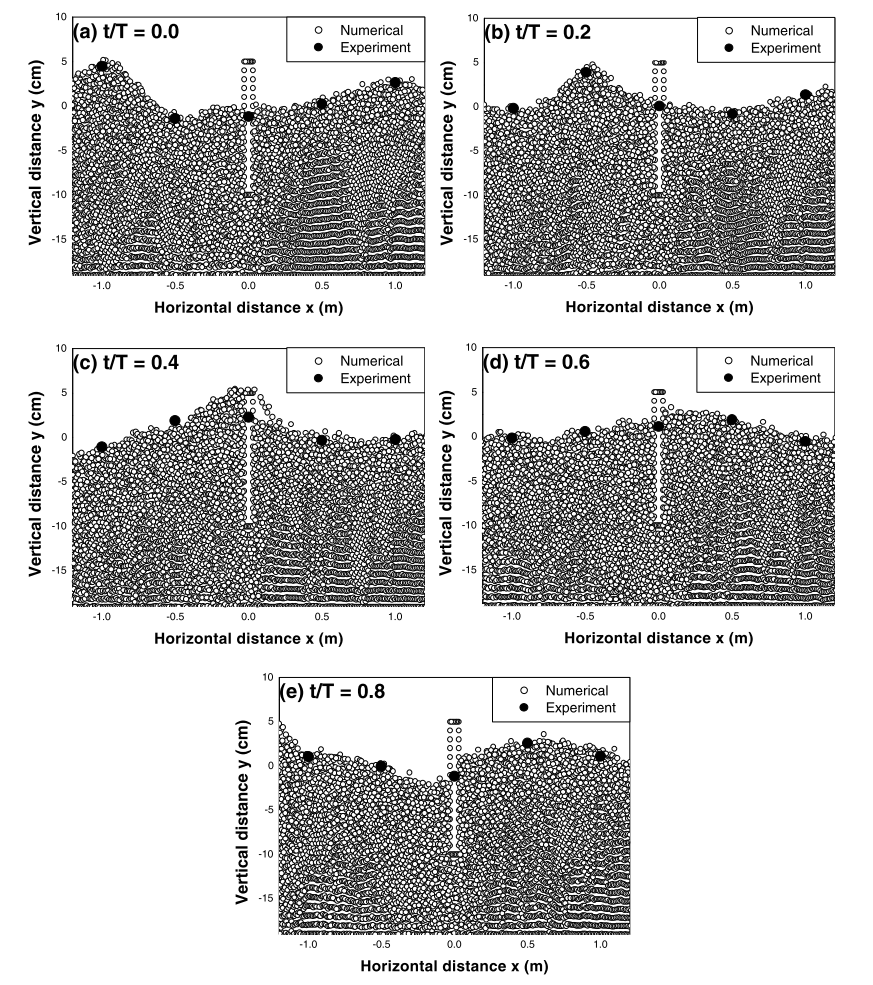
\includegraphics[width=12cm]{Figures/research_papers/gotoh2004-wave-profile-result.png}
    \caption{Time sequences of computational and experimental wave profiles near curtain wall (overtopping). Reproduced from \cite{Gotoh2004}}
    \label{fig:gotoh2004-wave-profile-result}
\end{figure}

As observed in the comparative plots given in \figref{fig:gotoh2004-wave-profile-result}, the model proves to be accurate in tracking free surfaces of large deformation without numerical diffusion. The authors also observed the model’s capability to simulate turbulence and eddy vortices realistically near the curtain wall. However, the authors also conclude that a more refined turbulence model will be required for further accuracy in predicting flow involving wave interactions.

Building on the work mentioned above, \cite{Shao2005} performed a comparative study of SPH and the Moving Particle Semi-Implicit (MPS) method coupled with an LES model. They also validated these models against experimental data.

The filtered conservation equations which the authors considered were the same as given by \Eqref{eq:Gotoh2004-continuity-filtered} - \Eqref{eq:Gotoh2004-boussinesq}. However, they incorporated the standard Smagorinsky model \parencite{smagorinsky1963general} given by \Eqref{eq:Shao2005-eddy-visc} as opposed to the modified model \Eqref{eq:Gotoh2004-eddy-visc}.
\begin{equation}
    \nu_t = (C_s \Delta x)^2
    \label{eq:Shao2005-eddy-visc}
\end{equation}

The authors consider the same predictive-corrective scheme to evolve their system as detailed in \Eqref{eq:Gotoh2004-predict-start} - \Eqref{eq:Gotoh2004-correct-end}.
Similarly, they follow the same SPH formulation outlined in \Eqref{eq:Gotoh2004-summation-density} - \Eqref{eq:Gotoh2004-vel-laplacian-sph}. They do however, slightly modify the pressure and velocity Laplacian terms as given in \Eqref{eq:Shao2005-P-laplacian-sph} and \Eqref{eq:Shao2005-vel-laplacian-sph} respectively.
\begin{equation}
    (\nabla^2 P)_i = \sum_j m_j \frac{4}{\rho_i + \rho_j} \frac{P_{ij} \RIJ \cdot \DWIJ }{\RtwoIJ}
    \label{eq:Shao2005-P-laplacian-sph}
\end{equation}
\begin{equation}
    \big(\nu \Delta(\vect{v}) \big)_i = \sum_j m_j \frac{2(\nu_i + \nu_j)}{\rho_i + \rho_j}\frac{\VIJ \RIJ \cdot \DWIJ}{\RtwoIJ}
    \label{eq:Shao2005-vel-laplacian-sph}
\end{equation}

The authors validated this SPH-LES Model using experimental data from the experimental data corresponding to a solitary wave breaking on the beach \parencite{Synolakis1986}. Their computational domain was $2D$ and consisted of $\approx \SciNot{1.8}{4}$ particles. 
From the computed wave profiles shown in \figref{fig:shao2005-wave-profile-result}, it can be visually observed that there is reasonable agreement between the experimental and computation data. This verifies the model’s accuracy in tracking free surfaces with less or no numerical diffusion.
Furthermore, by performing a convergence study of the SPH-LES model using the dam-break problem, the authors could show that the scheme’s spatial and temporal accuracy is $O(\Delta t + \Delta x^{1.25})$.

\begin{figure}[H]
    \centering
    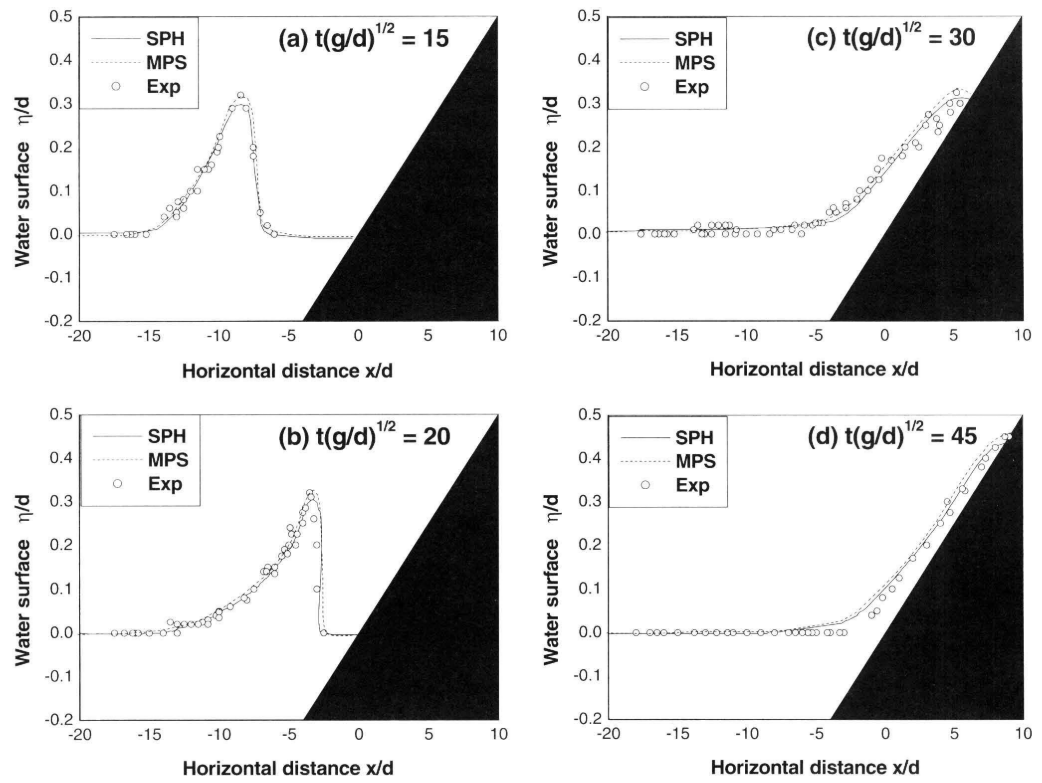
\includegraphics[scale=0.6]{Figures/research_papers/shao2005-wave-profile-result.png}
    \caption{Experimental and computational wave profiles by SPH and MPS model. Reproduced from \cite{Shao2005}}
    \label{fig:shao2005-wave-profile-result}
\end{figure}


\subsection{Explicit Pressure Equation of State-based Models}
\subsubsection{Standard Smagorinsky Model}

\cite{ROGERS2005}, similar to the work on SPH-LES modelling detailed in \secref{sec:Implicit-Pressure-Poisson-based-Models}, came up with an LES-type sub-particle-scale (SPS) formulation based on the weakly compressible assumption in order to develop a turbulence model for SPH.

The authors considered the mass and momentum conservation equations as already given in \Eqref{eq:Gotoh2004-continuity-governing} and  \Eqref{eq:Adami2012-mom-governing} respectively, along with the equation of state \Eqref{eq:violeau-eos}. However, for the value of $(B)$ in the state equation, the authors considered the definition given in \Eqref{eq:ROGERS2005-eos-b}:
\begin{equation}
    B' = 10 u_{max}
    \label{eq:ROGERS2005-eos-b}
\end{equation}
Where $(u_{max})$ is the maximum particle velocity.

They subsequently filtered the compressible conservation equations using Favre averaging as given by \Eqref{eq:ROGERS2005-favre-averaging}.
\begin{equation}
    \widetilde{f} = \frac{\overline{\rho f}}{\overline{\rho}}
    \label{eq:ROGERS2005-favre-averaging}
\end{equation}


The derived filtered conservation equations for mass and momentum are detailed in \Eqref{eq:ROGERS2005-continuity-filtered} and \Eqref{eq:ROGERS2005-mom-filtered}.
\begin{equation}
    \LagDerivative{\overline{\rho}} = -\overline{\rho} \nabla \cdot \vect{\widetilde{v}}
    \label{eq:ROGERS2005-continuity-filtered}
\end{equation}
\begin{equation}
    \LagDerivative{\vect{\widetilde{v}}} = - \frac{1}{\overline{\rho}}\nabla \overline{P} + \frac{1}{\overline{\rho}} (\nabla \cdot \overline{\rho \nu} \nabla) \vect{\widetilde{v}} + \frac{1}{\overline{\rho}}\nabla\cdot\tensor{\tau} + \vect{F}
    \label{eq:ROGERS2005-mom-filtered}
\end{equation}

Where the SPS stress tensor and turbulent eddy viscosity is given by \Eqref{eq:ROGERS2005-tau} and \Eqref{eq:ROGERS2005-turbulent-eddy-visc} respectively.
\begin{equation}
    \tensor{\tau} = \overline{\rho}\bigg(2\nu_t \tensor{S} - \frac{2}{3}\operatorname{tr}[\tensor{S}]\tensor{I}\bigg) - \frac{2}{3}\overline{\rho}C_I \overline{\Delta}^2 \tensor{I} \quad , \quad C_I = \SciNot{6.6}{-4}
    \label{eq:ROGERS2005-tau}
\end{equation}
\begin{equation}
    \nu_t = (C_s \Delta x)^2 \sqrt{2 \FrobeniusInnerProduct{S}{S}} \quad , \quad C_s = 0.12
    \label{eq:ROGERS2005-turbulent-eddy-visc}
\end{equation}

As for the SPH formulations of the aforementioned governing equations, the authors

The authors derived the SPH formulations of the aforementioned governing equations. The continuity equation takes the form as detailed in \Eqref{eq:violeau-continuity}. The pressure gradient term is given in \Eqref{eq:Gotoh2004-grad-p-sph}. The laminar stress term, consisting of the velocity Laplacian is given by \Eqref{eq:ROGERS2005-vel-laplacian-sph}, which itself was built on the work of \cite{morris1997modeling} as given in \Eqref{eq:morris1997modeling-vel-laplacian-sph}. Finally the stress divergence is defined by \Eqref{eq:Gotoh2004-div-tau-sph}.

\begin{equation}
    \bigg( \frac{1}{\rho} (\nabla \cdot \eta \nabla) \vect{v} \bigg)_i = \sum_j m_j \frac{\nu (\rho_i + \rho_i)}{\rho_{ij}^2} \frac{\VIJ \RIJ \cdot \DWIJ}{\RtwoIJ + \MachineEpsilon^2}
    \label{eq:ROGERS2005-vel-laplacian-sph}
\end{equation}
\begin{equation}
    \bigg( \frac{1}{\rho} (\nabla \cdot \eta \nabla) \vect{v} \bigg)_i = \sum_j m_j \frac{(\eta_i + \eta_j) \VIJ}{\rho_i \rho_j} \bigg( \frac{1}{\RtwoIJ[]} \PartialDerivative[r_i]{\WIJ} \bigg) \quad , \quad \DWIJ = \frac{\RIJ}{\RtwoIJ[]} \PartialDerivative[r_i]{\WIJ}
    \label{eq:morris1997modeling-vel-laplacian-sph}
\end{equation}

The authors noted that the LES description of viscous effects in slightly compressible SPH could lead to unphysical behaviour at free surfaces due to density variations being magnified by the equation of state. The lack of artificial viscosity implies that such variations are not damped. They subsequently noted that averaging the density would ensure smooth and physically acceptable free surfaces, based on the work of \cite{panizzo2004physical}. Hence, they performed Shepard filtering of the density as defined in \Eqref{eq:ROGERS2005-rho-shepard-filter} every 40-time steps.
\begin{equation}
    \rho_i = \frac{\sum_j \rho_j \WIJ \Vol_j}{\sum_j \WIJ \Vol_j}
    \label{eq:ROGERS2005-rho-shepard-filter}
\end{equation}

The authors simulated the problem of a weakly plunging breaker in $2D$ and $3D$ to ascertain the performance and capability of the model. Their $2D$ computational domain consisted of $\approx \SciNot{1}{5}$ particles, with the $3D$ domain consisting $\approx \SciNot{2}{4}$ particles.
The authors could show that in the case of the $2D$ problem, the model could predict regions of high vorticity that persisted longer when compared to standard SPH utilising conventional artificial viscosity. The model also displayed the turbulent bore, which generated reverse breaking, leading to the downbursting-like phenomenon, as observed in experiments \parencite{kubo2001large}.
In the case of the $3D$ problem, the authors showed the model’s capability to capture near vertically-oriented eddies despite the lower resolution. 

Building on this work, \cite{Dalrymple2006} used this scheme on a wide variety of problems, ranging from $2D$ Green water overtopping, $2D$ waves on a beach, $3D$ dam break and $3D$ waves on a beach. The quantitative analysis of the results allowed the authors to conclude that the model is especially suited for problems involving splash or flow separation. The authors also warn about the model’s requirement of a large number of particles for sufficient resolution. That and the finite speed of sound stemming from the compressible flow implied that time steps had to $O(10^{-5}s)$. Hence, the authors remain cautiously optimistic about the model since the method performs well for smaller regions where the number of particles is reasonable. However, they believe that extended Boussinesq codes would more efficiently model larger domains.

\subsubsection{Modified Smagorinsky Model}
\cite{Canelas2016} constructed the wall-adapting local eddy viscosity (WALE) model to be incorporated in the SPH-LES scheme. They noted that studying turbulent flow fields required the identification of vortices themselves to study their interactions in the flow. They used the definition of Lagrangian Coherent Structures (LCS) to help capture these vortices. As a Lagrangian method, SPH is preferable for studying LCS since the technique provides the motion of individual fluid particles, thereby eliminating the need for expensive post-processing inherent to Eulerian solutions. 
However, they noted that typically employed SPS strategies for LES simulations, based on the standard Smagorinsky model, cannot correctly enforce wall conditions and non-vanishing stresses with laminar flows. Hence they devised the WALE model.

The authors consider the compressible NS along the continuity equation as their governing equation. They subsequently present the SPH formulation of the continuity equation as defined by \Eqref{eq:Canelas2016-continuity-sph}.
\begin{equation}
    \LagDerivative{\rho_i} = - \rho_i \sum_j m_j \VIJ \cdot \DWIJ
    \label{eq:Canelas2016-continuity-sph}
\end{equation}
The pressure gradient term is given in \Eqref{eq:Gotoh2004-grad-p-sph}. The laminar stress term, consisting of the velocity Laplacian, is given by \Eqref{eq:Canelas2016-vel-laplacian-sph}. 
\begin{equation}
    \big(\nu \Delta(\vect{v}) \big)_i = \sum_j m_j \frac{4 \nu}{\rho_i + \rho_j}\frac{\VIJ \RIJ \cdot \DWIJ}{\RtwoIJ}
    \label{eq:Canelas2016-vel-laplacian-sph}
\end{equation}

Finally the stress divergence is defined by \Eqref{eq:Gotoh2004-div-tau-sph}, with the stress tensor being defined by \Eqref{eq:Canelas2016-tau}
\begin{equation}
    \tensor{\tau} = \rho \bigg( 2\nu_t \tensor{S} - \frac{2 \nu_t}{3}\operatorname{tr}[\tensor{S}]\tensor{I} \bigg) - \bigg( \frac{4}{3} \rho C_I (\Delta x)^2 \FrobeniusInnerProduct{S}{S} \bigg) \tensor{I} \quad , \quad C_I = \SciNot{6.6}{-3}
    \label{eq:Canelas2016-tau}
\end{equation}

The WALE model redefines the turbulent eddy viscosity as given by \Eqref{eq:Canelas2016-turbulent-eddy-visc}.
\begin{equation}
    \nu_t = \rho (C_w \Delta x)^2 \frac{\FrobeniusInnerProduct{S^d}{S^d}^{3/2}}{\FrobeniusInnerProduct{S}{S}^{5/2} + \FrobeniusInnerProduct{S^d}{S^d}^{5/4}} \quad , \quad C_w=0.325
    \label{eq:Canelas2016-turbulent-eddy-visc}
\end{equation}
\begin{equation}
    \tensor{S^d} = \HalfFrac \bigg( (\nabla \vect{v})^2 + \big((\nabla \vect{v})^T\big)^2 \bigg) - \frac{1}{3} \operatorname{tr}[(\nabla \vect{v})^2] \tensor{I}
\end{equation}

In order to test their model, the authors considered an array of cylinders in fluid flow as shown in \figref{fig:Canelas2016-vel-field}, with a constant body force. They computed the vorticity field and the Finite-Time Lyapunov Exponents (FTLE) field to study the LCSs in the flow. These fields are shown in \figref{fig:Canelas2016-vorticity-field} and \figref{fig:Canelas2016-ftle-field} respectively.

 \begin{figure}[H]
    \centering
    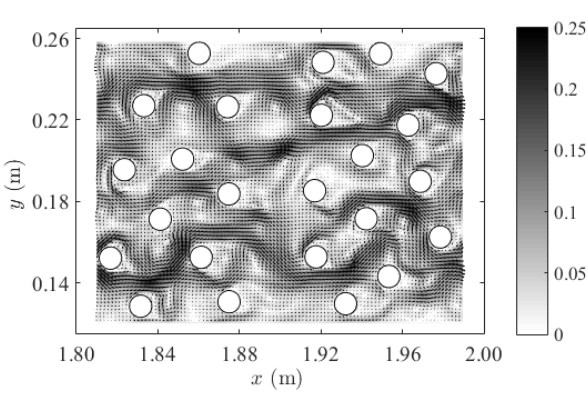
\includegraphics{Figures/research_papers/Canelas2016-vel-field.png}
    \caption{Cylinder distribution and instantaneous velocity overlapped by velocity vectors. Velocity in $m/s$, at $t=20s$. The flow direction is from left to right. Reproduced from \cite{Canelas2016}}
    \label{fig:Canelas2016-vel-field}
\end{figure}
\begin{figure}[H]
    \centering
    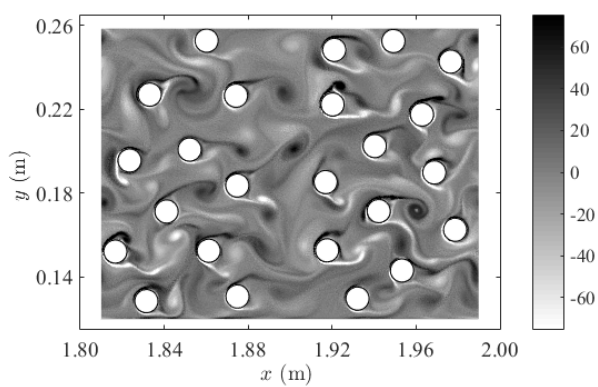
\includegraphics{Figures/research_papers/Canelas2016-vorticity-field.png}
    \caption{Vorticity field. Vorticity in Hz, at $t = 20s$. Reproduced from \cite{Canelas2016}}
    \label{fig:Canelas2016-vorticity-field}
\end{figure}
\begin{figure}[H]
    \centering
    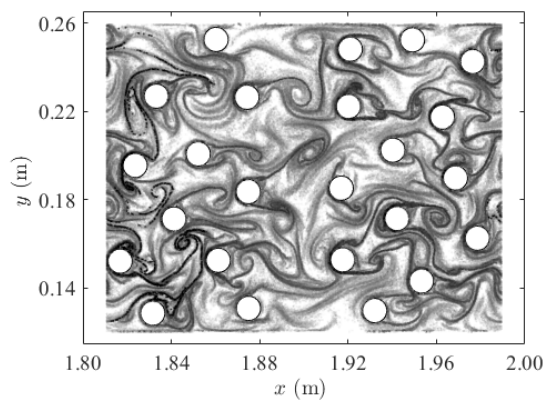
\includegraphics{Figures/research_papers/Canelas2016-ftle-field.png}
    \caption{FTLE field with negative integration time $(T = -0.4 s)$ (unstable manifolds - attracting LCS) at $t = 20s$. Reproduced from \cite{Canelas2016}}
    \label{fig:Canelas2016-ftle-field}
\end{figure}

The authors observed that the vortices produced, would evolve to recombine into larger structures. However, since vortex stretching is absent in $2D$, the authors believe that the recombination signifies \textit{energy injection} which leads to inverse cascade. They also observed that vortices with opposing strengths would interact and subsequently lead to vorticity cancellation. Hence, the authors note that such complex interactions lead to difficulties in interpreting the energy spectrum. Therefore, they believe that studies based on coherent structures would be required going forward.

\cite{Okraschevski2022}, building on the work of \cite{hardy1982formulas}, show that SPH should be viewed as a Lagrangian quadrature technique for the governing equations of explicit LES, raising interesting implications for SPH as a method itself. Firstly, the kernel scale limits SPH’s physical resolution, rendering it unsuitable as a DNS alternative. Secondly, any deficits introduced below the kernel scale could be resolved by consideration of the stress term, from which structures above the kernel scale could benefit. The authors consider this second implication a working hypothesis to try and prove or disprove.

The authors use the compressible NS equations and subject them to a spatial average operator to obtain the filtered governing equations. They subsequently derive the SPH formulations of the mass and momentum conservation equations as given in \Eqref{eq:Adami2012-summation-density} and \Eqref{eq:Okraschevski2022-mom-sph}.
\begin{equation}
    \overline{\rho}_i\LagDerivative{\widetilde{\vect{v}}} = - \sum_j (\overline{P}_i + \overline{P}_j) \DWIJ \Vol_j + 2(2+n_{dim})\eta \sum_j \frac{\widetilde{\vect{v}}_{ij} \cdot \RIJ}{\RtwoIJ}\DWIJ \Vol_j + \nabla \cdot \tensor{\tau}
    \label{eq:Okraschevski2022-mom-sph}
\end{equation}
Where $(n_{dim})$ denotes the number of spatial dimensions for a given problem.

The equation of state is given by \Eqref{eq:Okraschevski2022-eos-sph}, with the SFS tensor being given by \Eqref{eq:Okraschevski2022-tau}.
\begin{equation}
    \overline{P}_i = P_o + K\bigg(\frac{\overline{\rho}_i}{\rho_o} - 1 \bigg)
    \label{eq:Okraschevski2022-eos-sph}
\end{equation}
Where, $(K)$ is a constant.
\begin{equation}
    \tensor{\tau} = 2\nu_t\overline{\rho}\tensor{S}
    \label{eq:Okraschevski2022-tau}
\end{equation}

The SPH formulation for the strain rate tensor is given by \Eqref{eq:Okraschevski2022-S-tensor-sph}, and the divergence of the SFS tensor being given by \Eqref{eq:Okraschevski2022-div-tau-sph}.
\begin{equation}
    \tensor{S}_i = - \sum_j \widetilde{\vect{v}}_{ij} \otimes \DWIJ \Vol_j
    \label{eq:Okraschevski2022-S-tensor-sph}
\end{equation}
\begin{equation}
    \bigg(\nabla \cdot \tensor{\tau}\bigg)_i =\sum_j \big( \tensor{\tau}_i + \tensor{\tau}_j \big) \DWIJ \Vol_j
    \label{eq:Okraschevski2022-div-tau-sph}
\end{equation}

The authors consider three models for the turbulent eddy viscosity:
\begin{itemize}
    \item \texttt{SMAG}: Standard Smagorinsky model
        \begin{equation}
            \nu_t = (C_s \Delta x)^2 \sqrt{2 \FrobeniusInnerProduct{S}{S}}
            \label{eq:Okraschevski2022-SMAG}
        \end{equation}
        
    \item \texttt{SIGMA}: $\sigma$-model \parencite{nicoud2011using}, where $(\sigma_i)$ denotes the $i^{th}$ singular value of the velocity gradient
        \begin{equation}
            \nu_t = (C_{\sigma} \Delta x)^2 \frac{\sigma_3 (\sigma_1 - \sigma_2) (\sigma_2 - \sigma_3)}{\sigma_1^2}
            \label{eq:Okraschevski2022-SIGMA}
        \end{equation}
    
    \item \texttt{SMAG-MCG}: Standard Smagorinsky model discretized in the Monaghan-Cleary-Gingold (MCG) form \parencite{cleary1999conduction}
        \begin{equation}
            \nabla \cdot \tensor{\tau} = 2(2+n_{dim}) \sum_j \overline{\rho}_i \overline{\rho}_j \frac{\nu_{t, i} + \nu_{t, j}}{\overline{\rho}_i + \overline{\rho}_j} \frac{\widetilde{\vect{v}}_{ij} \cdot \RIJ }{\RtwoIJ} \DWIJ \Vol_j
            \label{eq:Okraschevski2022-SMAG-MCG}
        \end{equation}
\end{itemize}

The authors show a correlation between the vorticity and SFS tensor. They subsequently conclude that the fluctuations in the vorticity, energy spectra and SFS tensor are correlated quantities that contain different information about the numerical dissipation dynamics.

The authors use the $3D$ TGV problem to study and investigate the proposed models. They consider various resolutions to study the problem, varying from $\approx 200^3 - 500^3$ particles.
\begin{figure}[H]
    \centering
    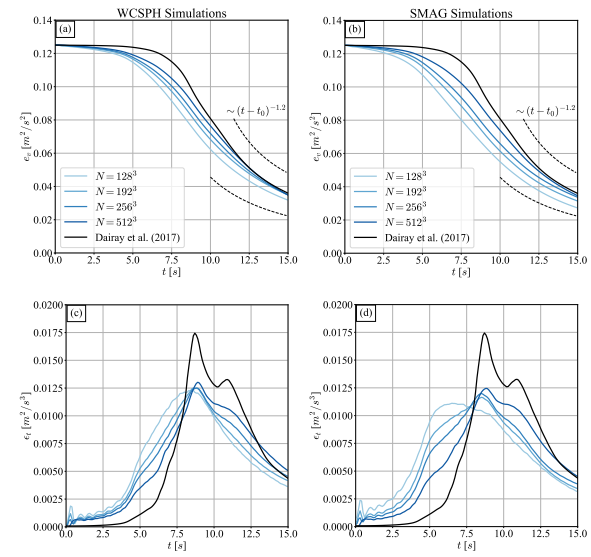
\includegraphics[scale=0.9]{Figures/research_papers/Okraschevski2022-fig-6.png}
    \caption{Comparison of quantitative metrics for different particle counts $N$. (a) \& (b) Temporal evolution of the density-weighted averaged kinetic energy. (c) \& (d) Temporal evolution of the averaged dissipation rate. Reproduced from \cite{Okraschevski2022}}
    \label{fig:Okraschevski2022-fig-6}
\end{figure}
\begin{figure}[H]
    \centering
    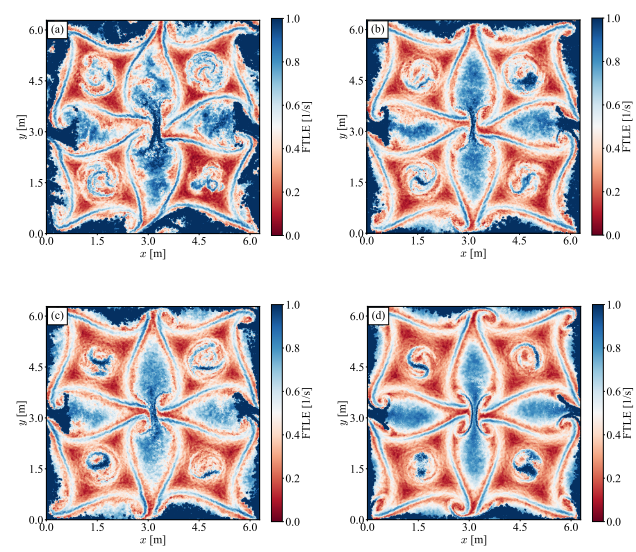
\includegraphics[scale=0.9]{Figures/research_papers/Okraschevski2022-fig-9.png}
    \caption{Backward FTLE at the plane $z =\pi$ for $N = 2563$ and $t = 14 s$ in the range $[11;14] s$. (a) Without explicit SFS model. (b) With the SMAG model. (c) With SIGMA model. (d) With the SMAG-MCG model. Reproduced from \cite{Okraschevski2022}}
    \label{fig:Okraschevski2022-fig-9}
\end{figure}
\begin{figure}[H]
    \centering
    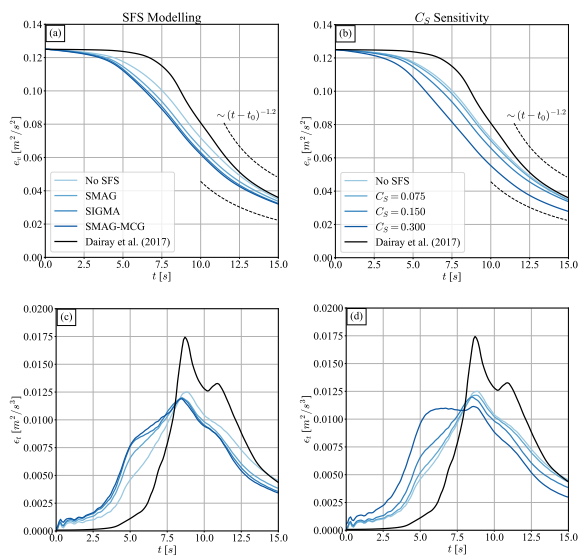
\includegraphics[scale=0.9]{Figures/research_papers/Okraschevski2022-fig-11.png}
	    \caption{Comparison of quantitative metrics for different $N = 256^3$ runs. (a) \& (b) Temporal evolution of the density-weighted averaged kinetic energy. (c) \& (d) Temporal evolution of the averaged dissipation rate. Reproduced from \cite{Okraschevski2022}}
    \label{fig:Okraschevski2022-fig-11}
\end{figure}

The \texttt{SMAG} model degrades the flow in terms of the averaged kinetic energy in \figref{fig:Okraschevski2022-fig-6} (b) and the corresponding dissipation rate in \figref{fig:Okraschevski2022-fig-6} (d). This negative attribute of the model outweighs the positive attribute of the model, in that cases with the SMAG model in \figref{fig:Okraschevski2022-fig-9} (b) appear less tattered and exhibit symmetry compared to the reference WCSPH solution in \figref{fig:Okraschevski2022-fig-9} (a).
From \figref{fig:Okraschevski2022-fig-11}, it becomes evident that with larger $(C_s)$, the averaged kinetic energy is increasingly reduced, which is also reflected by the dissipation rates. This indicates that the best choice corresponds to $(C_s \rightarrow 0)$.

On a concluding note, the authors claim that the subsonic turbulence captured by SPH can correctly represent the flow field up to the kernel scale but at a high cost in the best of cases. They also note that explicit SFS
models, at most, only lead to marginal improvement of LCS. However, regarding the inertial range dynamics, the dissipative SFS models remove kinetic energy, which is highly detrimental since a spectral energy deficit already characterises SPH. The authors attribute these drawbacks to the non-local character of the Lagrangian quadrature, which they explain through the concept of \textit{Particle Duality}. The concept states that the SPH particles must represent superfluid element approximants and fluid element surrogates simultaneously, leading to an unphysical increase in particle interaction distances. The authors, hence
prove Rennehen’s expectation that explicit SFS models in an SPH framework can only degrade the quality of the approximation for subsonic turbulent flow \parencite{rennehan2021mixing}, which raises concerns for turbulence modelling in SPH. However, the authors note there might be hope from SPH native models.
%TODO: Clean up the above part. Add more results?

%----------------------------------------------------------------------------------------
%	Section 3 - Lagrangian LES-based Models
%----------------------------------------------------------------------------------------
\section{Lagrangian LES-based Models}
\label{sec:lagrangian-les-based-model}
Having reviewed turbulence models developed for SPH, \cite{DiMascio2017} concluded that LES models could serve as an excellent middle ground between RANS and DNS. This is because only the sub-grid scale eddies would be modelled, allowing for the larger eddies to be directly simulated from the NS equations. They also note that contemporary SPH-LES models use the Eulerian differential operators in an SPH formulation and therefore do not have a rigorous background. Therefore they propose a Lagrangian form of LES to tie in with the Lagrangian quadrature technique, that is, SPH. 

The authors consider a weakly compressible, barotropic fluid whose conservation equations for mass and density are given by \Eqref{eq:Gotoh2004-continuity-governing} and \Eqref{eq:DiMascio2017-mom-governing} respectively.
\begin{equation}
    \LagDerivative{\vect{v}} = -\frac{1}{\rho} + \nu \Delta(\vect{v}) + (\lambda' + \nu)\nabla(\nabla \cdot \vect{v})
    \label{eq:DiMascio2017-mom-governing}
\end{equation}
Where, $(\lambda' = \lambda/\rho)$ is the Lam\'e constant.
The equation of state is simply given as \Eqref{eq:DiMascio2017-eos}.
\begin{equation}
    P = F(\rho)
    \label{eq:DiMascio2017-eos}
\end{equation}
\begin{equation}
    \LagDerivative{\vect{r}} = \vect{v}
    \label{eq:DiMascio2017-r-governing}
\end{equation}

The authors subsequently define a Lagrangian filter $(\phi)$ with compact support of the form
\begin{equation}
    \phi = \phi\big(\TildeR_p(t)-\vect{y}, t-\tau  \big)
    \label{eq:DiMascio2017-filter}
\end{equation}

Where the filter is an even function in its arguments, and $(\TildeR_p(t))$ is the position of a material which moves with velocity 
\begin{equation}
    \TildeV(\TildeR, t) = \IntRThreeAndT \phi \big(\TildeR_p(t)-\vect{y}, t-\tau  \big) \vect{v}(\vect{y}, \tau)d\tau dV_y
\end{equation}

By using the filter as defined in \Eqref{eq:DiMascio2017-filter}, the filtered governing equations are as follows
\begin{equation}
    \LagDerivative{\TildeRho} = -\TildeRho \nabla \cdot \TildeV + \nabla \cdot (\TildeRho\TildeV - \widetilde{\rho \vect{v}})
\end{equation}
\begin{equation}
    \LagDerivative{\TildeV} = - \frac{\nabla \TildeP}{\TildeRho} + \nu \Delta(\TildeV) + (\lambda'+\nu)\nabla(\nabla\cdot\TildeV) - \nabla[\widetilde{(\rho)}-G(\TildeRho)] + \nabla\cdot\tensor{T}_l+\widetilde{\vect{v}\nabla\cdot\vect{v}}
\end{equation}
\begin{equation}
    \LagDerivative{\TildeR}=\TildeV
\end{equation}
\begin{equation}
    \TildeRho = F(\TildeP)
\end{equation}
\begin{equation}
    \tensor{T}_l = \TildeV\otimes\TildeV - \widetilde{\vect{v}\otimes\vect{v}}
\end{equation}
\begin{equation}
    G(\rho) = \int^{\rho} \frac{1}{s}\frac{dF}{ds}ds
\end{equation}

In order for the authors to be able to reinterpret the Lagrangian LES through SPH, they split the filter as follows
\begin{equation}
    \phi\big(\TildeR_p(t)-\vect{y}, t-\tau  \big) = W(\TildeR - \vect{y})\theta(t-\tau)
\end{equation}

This allows the author to provide a relationship between the various type of filtered quantities as given
\begin{equation}
    \EncAngBrk{f}(\TildeR, t) = \int_{\mathbb{R}^3} W ( \TildeR - \vect{y} ) f ( \vect{y}, t ) dV_y
\end{equation}
\begin{equation}
    \bar{f}(\vect{y}, t) = \int_{\mathbb{R}} \theta(t-\tau) f(\vect{y}, \tau) d\tau
\end{equation}
\begin{equation}
    \widetilde{f} = \EncAngBrk{\bar{f}}, \EncAngBrk{\bar{f}} \neq \bar{\EncAngBrk{f}}
\end{equation}

The authors, therefore, can derive the equations in an SPH formalism as given by
\begin{equation}
    \LagDerivative{\TildeRho} = -\TildeRho \EncAngBrk{\nabla\cdot\TildeV} + C_1 + C_2
\end{equation}
\begin{equation}
    C_1 = -\TildeRho\EncAngBrk{\nabla\cdot(\bar{\vect{v}}-\TildeV)}
\end{equation}
\begin{equation}
    C_2 = \nabla\cdot(\TildeRho\TildeV - \widetilde{\rho\vect{v}})
\end{equation}
\begin{equation}
    \LagDerivative{\TildeV} = -\frac{\EncAngBrk{\nabla\TildeP}}{\TildeRho} + \nu\EncAngBrk{\Delta(\TildeV)} + (\lambda'+\nu)\EncAngBrk{\nabla(\nabla\cdot\TildeV)} + M_1 + M_2
\end{equation}
\begin{equation}
    M_1 = -\frac{\EncAngBrk{\nabla(\bar{\rho}-\TildeRho)}}{\TildeRho} + \nu\EncAngBrk{\Delta(\bar{\vect{v}}-\TildeV)} + (\lambda'+\nu)\EncAngBrk{\nabla(\nabla\cdot(\bar{\vect{v}}-\TildeV))}
\end{equation}
\begin{equation}
    M_2 = -\nabla\big(\widetilde{G(\rho)}-G(\TildeRho)\big) + \widetilde{\vect{v}\nabla\cdot\vect{v}} + \nabla\cdot\tensor{T}_l
\end{equation}
\begin{equation}
    \LagDerivative{\TildeR} = \TildeV
\end{equation}
\begin{equation}
    \TildeP=F(\TildeRho)
\end{equation}

The authors close the terms $(C_2, M_2)$ as follows
% \begin{equation}
%     C_1 \approx \TildeRho\EncAngBrk[\bigg]{\nabla\cdot\big(\sigma^2\Delta(\TildeV)\big)}, \sigma^2=h^2\alpha
% \end{equation}

% Where $(\alpha)$ is a dimensionless parameter.
\begin{equation}
    C_2 \approx \nabla \cdot (\nu_{\delta} \nabla\TildeRho)
\end{equation}
\begin{equation}
    \nu_{\delta} = (C_{\delta}\sigma)^2\sqrt{2\FrobeniusInnerProduct{S}{S}}
\end{equation}
Where $(\nu_{\delta})$ has the dimensions of kinematic viscosity and represents a turbulent diffusion coefficient, $(C_{\delta})$ represents a dimensionless coefficient, and $(\sigma \propto h)$. If the spatial derivative of $(\nu_{\delta})$ is negligible then
\begin{equation}
    C_2 = \nu_{\delta} \Delta(\TildeRho)
\end{equation}
\begin{equation}
    M_2 = \nabla \cdot \tensor{T}_l = \nabla \cdot \bigg( -\frac{k^2}{3}\tensor{I} - \frac{2}{3}\nu_t \operatorname{Tr}[\widetilde{\tensor{S}}]\tensor{I} + 2\nu_t\widetilde{\tensor{S}} \bigg)
\end{equation}
\begin{equation}
    k^2 = 4 C_y \sigma^2 \FrobeniusInnerProduct{S}{S} \quad , \quad C_y=0.044
\end{equation}
\begin{equation}
    \nu_t = (C_s\sigma)^2\sqrt{2 \FrobeniusInnerProduct{S}{S}} \quad , \quad C_s=0.12
\end{equation}
Where $(Tr[])$ is the trace operator, $(C_y)$ is the Yoshizawa constant \parencite{yoshizawa1986statistical}, and $(C_s$ is the Smagorinsky constant.

The above equations, coupled with the closure models, allow the authors to replace the differential operators with SPH counterparts of WCSPH.

The authors used the  $2D$ and $3D$ TGV problems to validate the model. The authors considered Reynolds number up to $\approx \SciNot{1.2}{5}$ for the $2D$ case, and $\approx \SciNot{1.5}{3}$ for the $3D$ case. The authors also compared the proposed model against that of the DNS SPH scheme, which was developed by \cite{mayrhofer2015dns} as observed in \figref{fig:DiMascio2017-fig-4} and \figref{fig:DiMascio2017-fig-9}.

\begin{figure}[H]
    \centering
    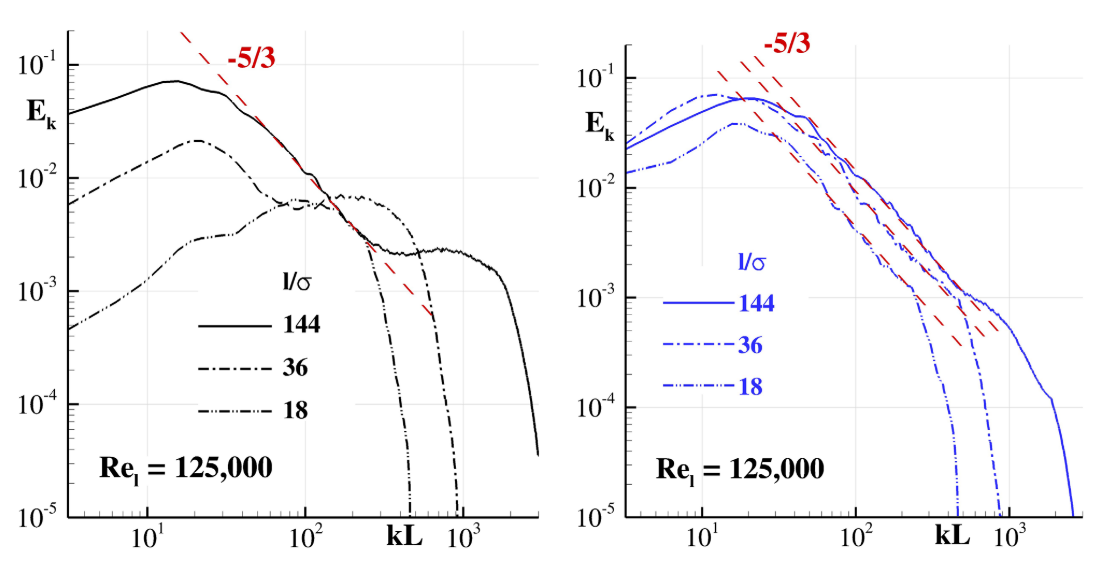
\includegraphics[scale=0.5]{Figures/research_papers/DiMascio2017-fig-4.png}
    \caption{$2D$ freely decaying turbulence $(tU/L = 2, Re = \SciNot{1.25}{5})$. Left: Energy spectrum using DNS-SPH. Right: Energy spectrum using LES- SPH. Reproduced from \cite{DiMascio2017}}
    \label{fig:DiMascio2017-fig-4}
\end{figure}
\begin{figure}[H]
    \centering
    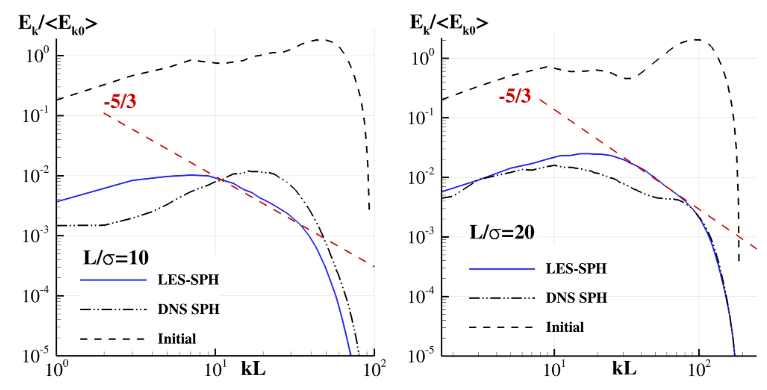
\includegraphics[scale=0.75]{Figures/research_papers/DiMascio2017-fig-9.png}
    \caption{$3D$ homogeneous turbulence decay. Comparison between DNS-SPH and LES-SPH simulations $(tU/L = 5)$. Left: Particle resolution = $64^3$. Right: particle resolution = $128^3$. Reproduced from \cite{DiMascio2017}}
    \label{fig:DiMascio2017-fig-9}
\end{figure}

 As seen from the results of the simulations in \figref{fig:DiMascio2017-fig-4} and \figref{fig:DiMascio2017-fig-9} for the $2D$ and $3D$ case, respectively, the authors were able to claim that the model captures the typical characteristics of the flow evolution with relatively coarse particle discretisation, provided an appropriate LES modelling is used.

Building on this, \cite{Colagrossi2021QuasiLagrangian} introduced a small arbitrary velocity deviation $(\TildeDeltaV)$ to the fluid particle as given by
\begin{equation}
    \LagDerivative{\TildeR} = \TildeV + \TildeDeltaV 
    \label{eq:Colagrossi2021QuasiLagrangian-r-transport}
\end{equation}

This was done since the Lagrangian nature of the proposed model was proving to be an obstacle for accurate simulations of high Reynolds number problems. Therefore, they modified the model with the transport equation given in \Eqref{eq:Colagrossi2021QuasiLagrangian-r-transport} to obtain a quasi-Lagrangian LES-SPH model. The small velocity deviation to the actual Lagrangian velocity was based on the work done on particle shifting technique (PST) and tensile instability control (TIC) technique by \cite{sun2018multi} in their $\delta$-SPH scheme.

The authors subsequently employed this $\delta$-LES-SPH scheme with the same set of closure models as detailed by \cite{DiMascio2017}. They compared their proposed model with standard LES-SPH on the $2D$ and $3D$ TGV problems for Reynolds numbers up to $\SciNot{1}{6}$.

\begin{figure}[H]
    \centering
    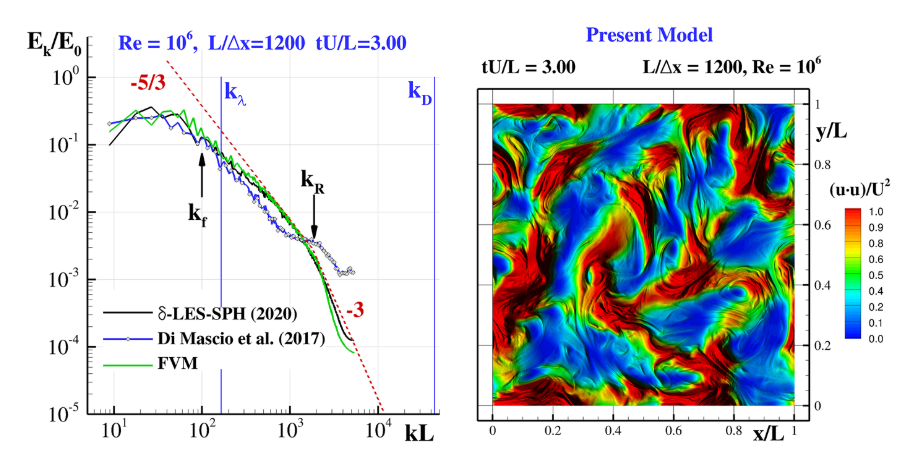
\includegraphics[scale=0.7]{Figures/research_papers/Colagrossi2021QuasiLagrangian-fig-4.png}
    \caption{Left: Energy spectrum at $(tU/L = 3, Re = \SciNot{1}{6})$ as predicted by the $\delta$-LES-SPH model and a finite volume scheme. Symbols $k_f$ and $k_R$ indicate the wave numbers of the external forcing and the kernel radius, respectively, while $k_{\lambda}$ and $k_D$ are the wave numbers associated with the Taylor and Kolmogorov scales. Right: $k$ field at the same instant. Reproduced from \cite{Colagrossi2021QuasiLagrangian}}
    \label{fig:Colagrossi2021QuasiLagrangian-fig-4}
\end{figure}
\begin{figure}[H]
    \centering
    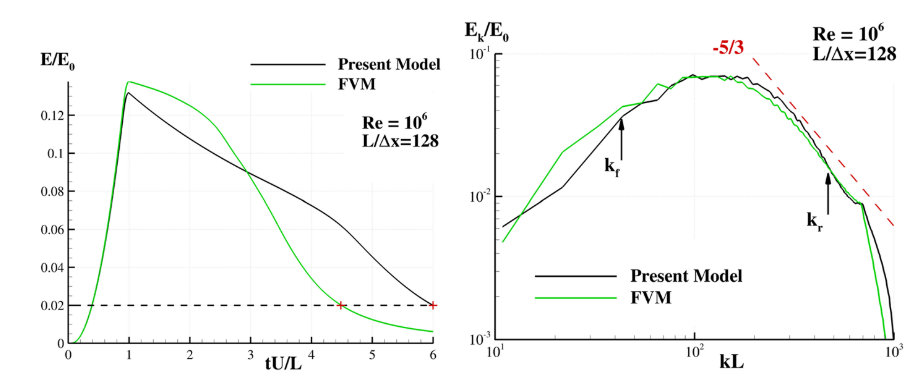
\includegraphics[scale=0.65]{Figures/research_papers/Colagrossi2021QuasiLagrangian-fig-8.png}
    \caption{Left: Time histories of $k$ as predicted by finite volume scheme and the $\delta$-LES-SPH model. Right: Energy spectra. Symbols $k_f$ and $k_R$ denote the wave numbers of the external forcing and the kernel radius, respectively. Reproduced from \cite{Colagrossi2021QuasiLagrangian}}
    \label{fig:Colagrossi2021QuasiLagrangian-fig-8}
\end{figure}

As seen from the results of the simulations in \figref{fig:Colagrossi2021QuasiLagrangian-fig-4} and \figref{fig:Colagrossi2021QuasiLagrangian-fig-8} for the $2D$ and $3D$ case respectively, the authors claimed that the proposed model could overcome issues of high Reynolds number flows, such as generation of spurious high-frequency noise and the onset of the tensile instability. Furthermore, comparing the proposed model’s and an FVM solve’s energy spectra with the theoretical decay rate confirmed the model’s accuracy and reliability.

The authors conclude that the $\delta$-LES-SPH model would need to be validated for flows with a Reynolds number larger than $\SciNot{1}{6}$ with experimental or numerical data. They believe that the inclusion of wall functions to deal with solid boundaries and the extension of the model to free-surface flows can further improve the model’s effectiveness. Finally, the authors believe that a higher-order approach could significantly improve the model results.

\subsection{Extension to EDAC-SPH Scheme}
\label{sec:Extension-to-EDAC-SPH-Scheme}
The Entropically Damped Artificial Compressibility (EDAC) SPH scheme, based on the work of \cite{Clausen2013}, is an explicit SPH method devised for incompressible flow by \cite{Ramachandran2019}.
In this scheme, the authors consider a transport equation for pressure instead of density derived from the continuity equation, as given in \Eqref{eq:Ramachandran2019-edac-p-transport}.
\begin{equation}
    \LagDerivative{P} = -c_s^2 \rho \nabla \cdot \vect{v} + \nu \nabla^2 P
    \label{eq:Ramachandran2019-edac-p-transport}
\end{equation}

Considering the pressure evolution equation above, an equation of state is longer required by the scheme.
By filtering \Eqref{eq:Ramachandran2019-edac-p-transport} with the Lagrangian LES technique \parencite{DiMascio2017}, we arrive at the result given by \Eqref{eq:edac-filtered} (Refer \appref{appendix:lagrangian-les-filtering-of-edac} for derivation).
\begin{equation}
    \LagDerivative{\TildeP} = -c_s^2 \rho \nabla \cdot \TildeV + \nu \nabla^2 \TildeP + \TildeV \cdot \nabla \TildeP - \widetilde{\vect{v}\cdot\nabla P}
    \label{eq:edac-filtered}
\end{equation}

In \Eqref{eq:edac-filtered}, we see that the term $(\widetilde{\vect{v}\cdot\nabla P})$ cannot be reduced further to a form of $(f(\TildeV, \TildeP))$. Hence, we cannot proceed with the SPH formulation for the pressure equation, implying that the EDAC scheme might not be compatible with the Lagrangian LES model.

%----------------------------------------------------------------------------------------
%	Section 4 - RANS-based $k-\epsilon$ Models
%----------------------------------------------------------------------------------------
\section[RANS-based k-epsilon Models]{RANS-based $k-\epsilon$ Models}
\label{sec:rans-based-k-epsilon-model}

\cite{Shao2006} demonstrated that the two-equation $k-\epsilon$ model, an extensively studied model derived from the Reynolds-averaged Navier–Stokes (RANS) equations, can be incorporated in the truly incompressible version of SPH (ISPH). By attempting to extend RANS equations, which are hugely successful in practical fields, to a mesh-free method such as SPH, the author provides a framework to build on the wide variety of closure models available.

To discretise the RANS equations to an SPH form, the author considers the Reynolds averaged mass and momentum conservation equations as given in \Eqref{eq:Shao2006-rans-continuity-governing} and \Eqref{eq:Shao2006-rans-mom-governing} respectively. \textit{Note:} The averaged flow properties are represented without any over-line $\overline{(...)}$ hereafter.
%TODO: Use filtered terms explicitly
\begin{equation}
    \frac{1}{\rho} \LagDerivative{\rho} + \nabla \cdot \vect{v} = 0 \quad , \quad \LagDerivative{\rho} = 0 \text{ (Incompressible)}
    \label{eq:Shao2006-rans-continuity-governing}
\end{equation}
\begin{equation}
    \LagDerivative{\vect{v}} = -\frac{1}{\rho}\nabla P + \nu \Delta( \vect{v} ) + \frac{1}{\rho} \nabla \cdot \tensor{\tau} + \vect{F}
    \label{eq:Shao2006-rans-mom-governing}
\end{equation}

The stress tensor is given by \Eqref{eq:Gotoh2004-boussinesq}, while the turbulent eddy viscosity is defined as \Eqref{eq:Shao2006-turbulent-eddy-visc}.
\begin{equation}
    \nu_t = c_d \frac{k^2}{\epsilon}
    \label{eq:Shao2006-turbulent-eddy-visc}
\end{equation}

The transport equations for the turbulent kinetic energy and dissipation rate is given by \Eqref{eq:Shao2006-k-transport-eq} and \Eqref{eq:Shao2006-eps-transport-eq} respectively.
\begin{equation}
    \LagDerivative{k} = \nabla \cdot \bigg( \frac{\nu_t}{\sigma_k} \nabla k \bigg) + P_k - \epsilon
    \label{eq:Shao2006-k-transport-eq}
\end{equation}
\begin{equation}
    \LagDerivative{\epsilon} = \nabla \cdot \bigg( \frac{\nu_t}{\sigma_{\epsilon}} \nabla \epsilon \bigg) + c_{1\epsilon} \frac{\epsilon}{k} P_k - c_{2\epsilon} \frac{\epsilon^2}{k}
    \label{eq:Shao2006-eps-transport-eq}
\end{equation}
\begin{equation}
    P_k = 2\nu_t \FrobeniusInnerProduct{S}{S}
    \label{eq:Shao2006-k-production-term}
\end{equation}

Where, $(\sigma_k, \sigma_{\epsilon}, c_{1\epsilon}, c_{2\epsilon}) = (1.0, 1.3, 1.44, 1.92)$ are empirical constants dependent on the nature of the flow , and $(P_k)$ is the turbulence production rate, which satisfies the relation given by \Eqref{eq:pope2000turbulent-k-production-relation} \parencite{pope2000turbulent}.
\begin{equation}
    \frac{P_k}{\epsilon} = c_d \Bigg( \frac{\sqrt{2 \FrobeniusInnerProduct{S}{S}}}{\epsilon} \Bigg)
    \label{eq:pope2000turbulent-k-production-relation}
\end{equation}

These governing equations are solved and evolved using the same predictive-corrective time integrator as seen in the work of \cite{Gotoh2004}, and outlined in \Eqref{eq:Gotoh2004-predict-start} - \Eqref{eq:Gotoh2004-correct-end}.

As for the SPH formulations of the governing equations, the author builds on the work of \cite{Gotoh2004}, and uses the same discretization as defined in \Eqref{eq:Gotoh2004-summation-density} - \Eqref{eq:Gotoh2004-div-tau-sph}. However, the author uses a slightly modified version of the laminar stress term given in \Eqref{eq:Gotoh2004-vel-laplacian-sph} and redefines it as given in \Eqref{eq:Shao2006-vel-laplacian-sph}.
\begin{equation}
    \big(\nu \Delta(\vect{v}) \big)_i = \sum_j m_j \frac{2 ( \nu_i + \nu_j ) }{ \rho_i + \rho_j }\frac{\VIJ \RIJ \cdot \DWIJ}{\RtwoIJ}
    \label{eq:Shao2006-vel-laplacian-sph}
\end{equation}

The author tested the model on the problem of $2D$ wave breaking and overtopping of a sloping wall and compared the results obtained against the experimental data from the work of \cite{li2004wave} to validate the model—the computational domain of $\approx \SciNot{6}{3}$ particles.

As seen from the evolution of the water surface elevation plotted in \figref{fig:Shao2006-water-surf-elevations}, the author could ascertain that the proposed model produced better results than those of \cite{li2004wave}, compared to the experimental data in \figref{fig:Shao2006-water-surf-elevations}(a) and \figref{fig:Shao2006-water-surf-elevations}(b). This could be attributed to the free surfaces being accurately tracked by particles without numerical diffusion. 
In \figref{fig:Shao2006-water-surf-elevations}(c) and \figref{fig:Shao2006-water-surf-elevations}(d), despite the wave profiles being consistent with each other in phase and shape, the proposed model predicts smaller elevation levels. Li et al. use a dynamic Smagorinsky model, whereas the proposed model uses constant empirical coefficients. The author believes these coefficients derived from a quasi-steady state may behave sub-optimally in transient flow, such as the problem at hand.
\begin{figure}[H]
    \centering
    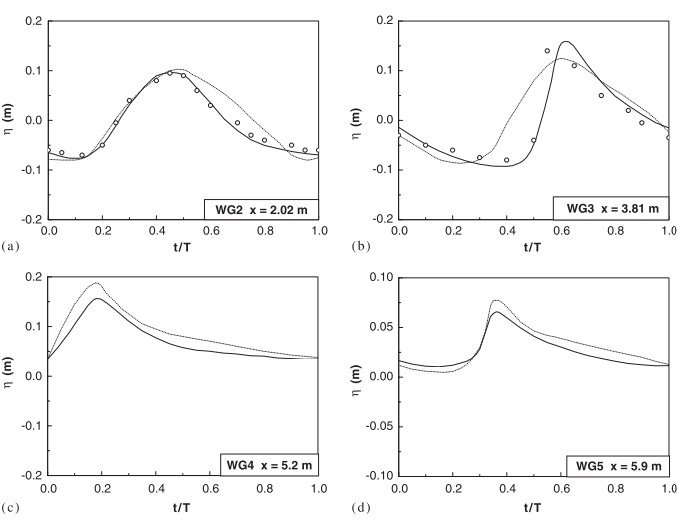
\includegraphics[scale=0.9]{Figures/research_papers/Shao2006-water-surf-elevations.png}
    \caption{Comparisons of computed water surface elevations by SPH (solid lines) with experimental ($\circ$) and numerical (dotted lines) data of \cite{li2004wave}. Reproduced from \cite{Shao2006}}
    \label{fig:Shao2006-water-surf-elevations}
\end{figure}

The author concludes that the $k-\epsilon$ model would require further sensitivity analysis for the turbulence model and spatial resolution for improved results, despite being reasonably accurate in tracking free surfaces.

\cite{Wang2020} build on the work of \cite{Shao2006} to further improve the ISPH $k-\epsilon$ model. They achieved this by using the modelling and computational developments which SPH has benefited from since the work of Shao.
The authors here consider the same SPH discretised equations and two-step time integrator as Shao, with two distinct modifications in the Pressure Poisson equation as given by \Eqref{eq:Wang2020-correct-pressure-implicit} instead of \Eqref{eq:Gotoh2004-correct-pressure-implicit}. They also redefined propagation equation for $(\vect{r}$ using \Eqref{eq:Wang2020-correct-end} instead of \Eqref{eq:Gotoh2004-correct-end}.
\begin{equation}
    \nabla \cdot \bigg( \frac{1}{\rho_o} \nabla P_{t+1} \bigg) = \frac{1}{\Delta t} \nabla \cdot \vect{u_*}
    \label{eq:Wang2020-correct-pressure-implicit}
\end{equation}
\begin{equation}
    \vect{r}_{t+1} = \vect{r}_* + \Delta \vect{v}_{**} \Delta t
    \label{eq:Wang2020-correct-end}
\end{equation}

The authors also provided SPH discretization for the transport equations for $(k)$ and $(\epsilon)$ using \Eqref{eq:Wang2020-k-laplacian} and \Eqref{eq:Wang2020-eps-laplacian} which requires the use of particle density $(\varphi)$ as given in \Eqref{eq:Wang2020-particle-density}.
\begin{equation}
    \varphi_i = \sum_j \WIJ
    \label{eq:Wang2020-particle-density}
\end{equation}
\begin{equation}
    \nabla \cdot \bigg( \frac{\nu_t}{\sigma_k} \nabla k \bigg)_i = - \sum_j \frac{1}{\varphi_j} \bigg( \frac{\nu_{t,i}}{\sigma_k} + \frac{\nu_{t,i}}{\sigma_k}  \bigg) \frac{k_{ij} \RIJ \DWIJ}{\RtwoIJ}
    \label{eq:Wang2020-k-laplacian}
\end{equation}
\begin{equation}
    \nabla \cdot \bigg( \frac{\nu_t}{\sigma_{\epsilon}} \nabla \epsilon \bigg)_i = - \sum_j \frac{1}{\varphi_j} \bigg( \frac{\nu_{t,i}}{\sigma_{\epsilon}} + \frac{\nu_{t,i}}{\sigma_{\epsilon}}  \bigg) \frac{\epsilon_{ij} \RIJ \DWIJ}{\RtwoIJ}
    \label{eq:Wang2020-eps-laplacian}
\end{equation}

The authors also derived an SPH formulation for the strain rate tensor defined in \Eqref{eq:Wang2020-strain-rate-tensor}, which is based on the studies done on kernel correction \parencite{bonet1999variational, khayyer2008corrected} and given by \Eqref{eq:Wang2020-vel-grad-term} and \Eqref{eq:Wang2020-corrective-matrix}. 
\begin{equation}
    \tensor{S}_i = \HalfFrac \bigg( \nabla \vect{v}_i + (\nabla \vect{v}_i)^T \bigg)
    \label{eq:Wang2020-strain-rate-tensor}
\end{equation}
\begin{equation}
    \nabla \vect{v}_i = - \sum_j \frac{1}{\varphi_j} \VIJ \otimes \tensor{L}_i \DWIJ
    \label{eq:Wang2020-vel-grad-term}
\end{equation}
\begin{equation}
    \tensor{L}_i = \Bigg(- \sum_j \frac{1}{\varphi_j} \DWIJ \otimes \RIJ \Bigg)^{-1}
    \label{eq:Wang2020-corrective-matrix}
\end{equation}

The authors validated the model against the problem of a solitary wave propagating over a bottom-mounted barrier in $2D$. Its results are shown in \figref{fig:Wang2020-wave-propogation-result}. They also considered the problem involving wave breaking on a slopping wall in $2D$, which is shown in \figref{fig:Wang2020-wave-breaking-result}.
\begin{figure}[H]
    \centering
    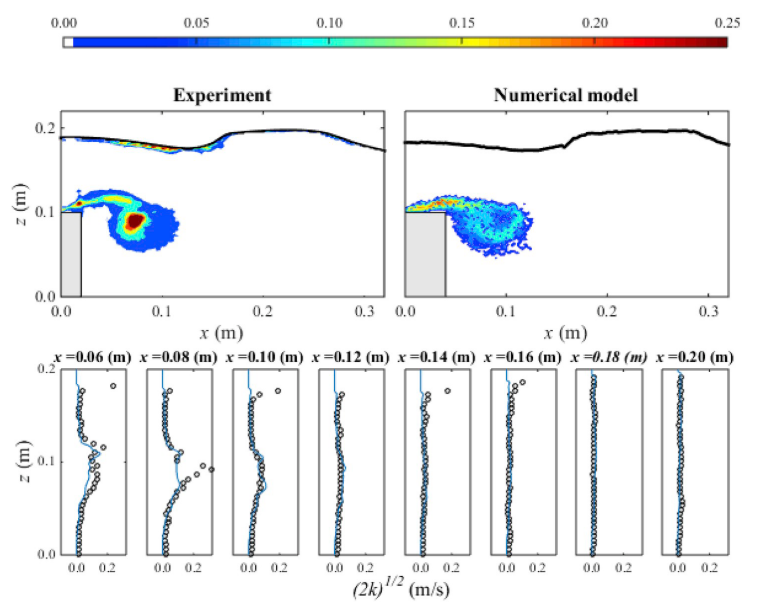
\includegraphics[scale=0.75]{Figures/research_papers/Wang2020-wave-propogation-result.png}
    \caption{Comparisons between experimental data (left) and numerical results (right) for turbulence intensity $(m/s)$ at $t=0.6s$ (top panels) and the corresponding vertical cross-sections (lower panels). In the lower panels, solid lines and $\circ$ represent the numerical and experimental results, respectively. Reproduced from \cite{Wang2020}}
    \label{fig:Wang2020-wave-propogation-result}
\end{figure}
\begin{figure}[H]
    \centering
    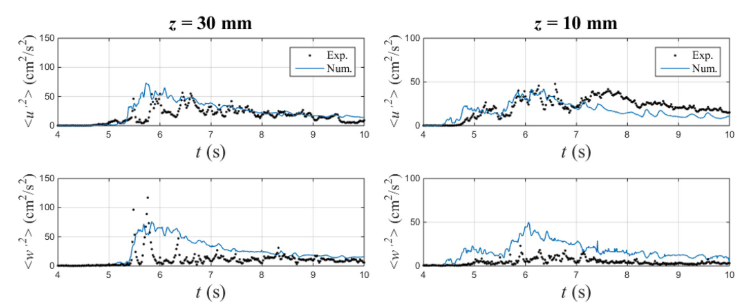
\includegraphics[scale=0.8]{Figures/research_papers/Wang2020-wave-breaking-result.png}
    \caption{Comparisons of numerical and experimental turbulent kinetic energy in x-direction and y-direction. Reproduced from \cite{Wang2020}}
    \label{fig:Wang2020-wave-breaking-result}
\end{figure}

Given the model’s accuracy, as observed from the figures, the authors conclude that the model’s capabilities have been demonstrated, especially in tracking transient-free surfaces. They also reproduce the evolution of turbulence and its intensity due to flow separation. 
However, they note that the model under-predicts the max turbulent kinetic energy and is sensitive to the initial seeding of the turbulent kinetic energy property.
The authors also state that the counteracting effects of the physical viscous dissipation and numerical dissipation, dependent on the particle resolution, would have to be appropriately balanced.
Finally, the authors conclude on the importance of boundary treatment and the need for more sophisticated boundary models to extend the model to $3D$ domains.

%TODO: Need to include Wang2022.

%----------------------------------------------------------------------------------------
%	Section 5 - LANS-based Models
%----------------------------------------------------------------------------------------
\section{LANS-based Models}
\label{sec:lans-based-model}
So far, having dealt with RANS and LES models of turbulence, a few fundamental drawbacks of these techniques have been brought to light.
In the case of RANS, the flow field is decomposed into
an averaged mean flow and a fluctuating field. Such a decomposition of the NS equations provides differential equations for the mean flow containing contributions from the time-varying turbulent motion. Therefore a closure model is required to capture the effects of the fluctuations on the mean flow. However, by studying only the mean flow quantities, the complete nature of the flow, notwithstanding the complex structures stemming from these fluctuations, cannot be studied, let alone appreciated.

On the face of it, LES would have made for a reasonable alternative to model turbulent flows. This is because the large scales in the flow are resolved by the standard NS equations, while the effects of smaller scales are modelled. However, this remains easier said than done since inhomogeneous and wall-bounded flows necessitate the LES filter width to vary dynamically to capture the average size of turbulent eddies.

The other widespread method of tackling turbulence involves Direct Numerical Simulation (DNS). However, since the number of degrees of freedom for a $3D$ flow grows rapidly with the Reynolds number $(\propto Re^{9/4})$, this technique effectively places an inviolable upper bound on the $Re$ for a given simulation because of computational limitations.

In order to tackle the issues above and address them reasonably, we look for possible solutions. One such solution is the Lagrangian averaging method introduced by \cite{holm1998euler} and \cite{Marsden2001}. In this method, unlike the averaging or filtering of the NS equations as done in RANS or LES, the Lagrangian averaging approach averages at the level of the variational principle from which the Navier–Stokes equations are derived. This procedure yields the Lagrangian-averaged Navier Stokes-$\alpha$ (LANS-$\alpha$) equations, which describe the time evolution of large eddies in turbulent flows. It can be stated that this approach is similar to that of LES.

The LANS-$\alpha$ equations, assuming incompressibility and isotropic turbulence, are derived and simplified by \cite{Mohseni2003}. These equations are as follows:
\begin{equation}
    \nabla \cdot \vect{v} = 0
\end{equation}
\begin{equation}
    \LagDerivative{\vect{v}} = \tensor{\sigma}(\vect{v})
\end{equation}
\begin{equation}
    \tensor{\sigma}(\vect{v}) = -P\tensor{I} + 2\nu(1 - \alpha^2\Delta)\tensor{S} + 2\alpha^2\Dot{\tensor{S}}
\end{equation}
\begin{equation}
    \Dot{\tensor{S}} = \LagDerivative{\tensor{S}} + \tensor{S}\tensor{R} - \tensor{R}\tensor{S}
\end{equation}
\begin{equation}
    \tensor{R} = \HalfFrac\bigg(\nabla\vect{v}-(\nabla\vect{v})^T\bigg)
\end{equation}
Where $\alpha$ denotes the scale of rapid fluctuations in the flow map, such that for scales smaller than $\alpha$, the wave activity is filtered by a nonlinear energy redistribution. Here, $(1 - \alpha^2 \Delta)$ denotes the Helmholtz operator.

\cite{Monaghan2002}, building on the work of \cite{holm1998euler}, attempted to formulate an SPH version of the continuum LANS-$\alpha$ equations. His work provided one of the earliest models of turbulence in compressible flow. The author incorporated some of his earlier work on XSPH \parencite{monaghan1989problem}, in which particles are moved with a smoothed velocity, leaving the acceleration equation unchanged. The smoothed velocity denoted an average over the velocities of the neighbouring particles. This facilitated the author in writing the Lagrangian analysed by Holm in an SPH form, allowing for the subsequent derivation of the momentum equation, albeit being elaborate and highly complicated. Nevertheless, in conjunction with the continuity equation, the derived momentum equation formulated the SPH-$\alpha$ model, which essentially consisted of an SPH particle moving with the transport velocity smoothed from momentum velocity by an iterative algorithm with an additional dissipation term meant to mimic the standard LES model.

\cite{Hu2015} also devised a turbulence model for incompressible flow based on spatial filtering of the NS equations using SPH approximations termed the SPH-$\sigma$ model. The model shares similarities with the LANS-$\alpha$ model and the SPH-$\alpha$ model, differing by the additional stress term in the model and its approach in evaluating the particle transport velocity. The proposed model is also built on the authors’ previous work \parencite{hu2007incompressible}, and hence shares similar numerical techniques. The authors also validated the proposed model on $2D$ flow comprising decaying and forced turbulence cases. Their results suggested that the model could simulate incompressible turbulent flow.

Monaghan \parencite{Monaghan2011, Monaghan2017} subsequently improved on the SPH-$\alpha$ model and derived a more amenable variant of the momentum equation. Since, in this case, the model was parameterised around the smoothing parameter $(\varepsilon)$, the turbulence model was termed the SPH-$\varepsilon$ model. The linearly smoothed velocity $(\widehat{\vect{v}})$ is given by \Eqref{eq:Monaghan2017-xsph-vel-smoothing}.
\begin{equation}
    \widehat{\vect{v}}_i = \vect{v}_i - \varepsilon \sum_j \frac{m_j}{M_o} \VIJ K_{h', ij} \quad , \quad \varepsilon \in [0, 1]
    \label{eq:Monaghan2017-xsph-vel-smoothing}
\end{equation}
Where $(K)$ is a smoothing kernel, which can be different from the kernel used in SPH, its corresponding smoothing length being $(h')$. It is noted that the smoothed velocity preserves the shape of the spectrum of the unsmoothed velocity for short-length scales. However, it reduces the magnitude of the unsmoothed velocity by a factor $(1-\varepsilon)$. 

The equation of state is given by \Eqref{eq:violeau-eos}, and the momentum equation is given by \Eqref{eq:Monaghan2017-mom-governing}. The momentum equation’s third term on the right-hand side is an extra stress term determined by the smoothing. Its overall effect is to redistribute energy without dissipation.
\begin{equation}
    \LagDerivative{\vect{v}_i} = - \sum_j m_j \bigg( \frac{P_i}{\rho_i^2} + \frac{P_j}{\rho_j^2} \bigg) \DWIJ - \sum_j m_j \Pi_{ij} \DWIJ + \frac{\varepsilon}{2} \sum_j \frac{m_j}{M_o} \VtwoIJ[] \DWIJ 
    \label{eq:Monaghan2017-mom-governing}
\end{equation}
Where the viscosity term $(\Pi_{ij})$ is given by \Eqref{eq:Monaghan2017-Pi-visc-term}, in which $(\alpha)$ is a constant.
\begin{equation}
    \Pi_{ij} = - \frac{2 \alpha c_s \VIJ \cdot \RIJ}{(\rho_i + \rho_j) \RtwoIJ}
    \label{eq:Monaghan2017-Pi-visc-term}
\end{equation}

The particles are subsequently transported using \Eqref{eq:Monaghan2017-r-transport}.
\begin{equation}
    \LagDerivative{\vect{r}_i} = \widehat{\vect{v}}_i
    \label{eq:Monaghan2017-r-transport}
\end{equation}

The author validated the proposed model by simulating $2D$ flow past a cylinder moving along a Lissajous curve.
The author demonstrated the model’s capabilities to predict satisfactory results for the velocity correlation functions, energy spectrum and mixing while having particle resolution be half of that required for a DNS with a resolution the Reynolds length. The author concludes that the model’s effectiveness for higher Reynolds numbers and other boundary conditions, such as free surfaces, will need to be studied further.

%----------------------------------------------------------------------------------------
%	Section 6 - Miscellaneous Models
%----------------------------------------------------------------------------------------
\section{Miscellaneous Models}
\cite{Liu2019} approached the problem of turbulence modelling from the perspective of computer $3D$ visualisation to visualise flows with realistic features. The authors’ viscosity-based vorticity correction model offers more advantages to the computer visual-effects audience. However, the model would still be a worthwhile investigation.

The authors define a vorticity field $(\Vorticity)$ in the system as given in \Eqref{eq:Liu2019-vorticity}.
\begin{equation}
    \Vorticity_i = \nabla \times \vect{v}_i = - \frac{1}{\rho} \sum_j m_j \VIJ \times \DWIJ
    \label{eq:Liu2019-vorticity}
\end{equation}

The contribution to the SPH particle’s momentum velocity from the viscous term is calculated as given in \Eqref{eq:Liu2019-visc-vel-contribution}.
\begin{equation}
    \vect{v}_{\nu, i} = \vect{v}_i + \vect{a}_i^{(visc)}\Delta t
    \label{eq:Liu2019-visc-vel-contribution}
\end{equation}
If the magnitude of viscous velocity $(\vect{v}_{\nu, i})$ is greater than $(\vect{v}_i)$ for a given particle, then its vorticity field is updated as given in \Eqref{eq:Liu2019-vorticity-update}.
\begin{equation}
    \delta \Vorticity_i = (\alpha \sqrt{R_i}) \Vorticity_i
    \label{eq:Liu2019-vorticity-update}
\end{equation}
\begin{equation}
    R_i = \frac{\delta E_i}{E_i} = \frac{\vect{v}_{\nu, i}^2 - \vect{v}_i^2}{\vect{v}_i^2}
    \label{eg:Liu2019-R}
\end{equation}

A stream function $(\Psi)$ is subsequently defined as given in \Eqref{eq:Liu2019-stream-func}.
\begin{equation}
    \Psi_i = \sum_j \frac{\delta \Vorticity_j \Vol_j}{4\pi \RtwoIJ[]}
    \label{eq:Liu2019-stream-func}
\end{equation}

The velocity correction $(\delta \vect{v})$ for the particle is subsequently defined by \Eqref{eq:Liu2019-vel-update}.
\begin{equation}
    \delta \vect{v}_i = \nabla \times \Psi_i
    \label{eq:Liu2019-vel-update}
\end{equation}

\cite{Obeidat2018}, tackle the problem of turbulence by devising a hybrid remeshed method (hrSPH)
for the simulation of three-dimensional turbulent flows. 
The authors essentially use an Eulerian mesh with Lagrangian particles to gain advantages of both schemes. The governing equations are evaluated using the properties at the mesh nodes, which are interpolated from the particles. After evaluating the system of equations, the new properties on the mesh nodes are used to update the properties of the particles through mesh-to-particle interpolation. The authors consider the turbulent sub-grid stresses using the Smagorinsky model.

The proposed model remeshes the particles when the distribution is not uniform. The authors validated the model against the $2D$ and $3D$ TGV problems, thin double shear layer problems, and $3D$ isotropic turbulence obtained from DNS. The model predicts the energy spectra and energy dissipation reasonably well. Despite the model’s accuracy, not much information can be gathered to help solely improve the state of turbulence modelling in SPH.
% Chapter 3

\chapter{Evaluation of Turbulence Models}

\label{chap:evaluation-of-turbulence-models}

Turbulence, as a phenomenon, has been notoriously difficult for a detailed physical analysis. This is further exacerbated by the seemingly endless complex interactions it gives rise to in the flow as long as any form of energy is provided.
Therefore, while modelling turbulence remains one facet of the problem, visualising and analysing the model is another equally challenging task.

As seen in the previous \chapref{chap:turbulence-modelling}, numerous Lagrangian turbulent models seem to be tested for only complex surface flows. However, a systematic analysis of isotropic turbulence problems provides greater insight into the energy spectrum and its corresponding cascade across varying length scales. A reasonable model should be able to capture the characteristic hierarchy of scales through which the energy cascade takes place. The dissipation of kinetic energy finally occurs at the scales of the order of Kolmogorov length, where the flow subsequently becomes laminar. In contrast, the injection of energy in turbulent flow generally occurs at much larger scales.

Hence, appropriate test cases must be used when analysing turbulence.

%----------------------------------------------------------------------------------------
%	Section 1 - Benchmark Problems
%----------------------------------------------------------------------------------------
\section{Benchmark Problems}
\subsection{Taylor-Green Vortex Problem}
The Taylor-Green vortex problem is a challenging case to tackle. The flow is periodic, incompressible and consists of decaying vortices.
The $2D$ case of the problem is analytically defined as given by \Eqref{eq:2d-tgv-vx} - \Eqref{eq:2d-tgv-p}.
\begin{equation}
    v_x = -U e^{bt} \cos(2\pi x) \sin(2\pi y)
    \label{eq:2d-tgv-vx}
\end{equation}
\begin{equation}
    v_y = U e^{bt} \sin(2\pi x) \cos(2\pi y)
    \label{eq:2d-tgv-vy}
\end{equation}
\begin{equation}
    p = (U e^{bt})^2 \frac{\cos(4\pi x) + \cos(4\pi y)}{4}
    \label{eq:2d-tgv-p}
\end{equation}
\begin{equation}
    b = -\frac{8\pi}{Re} \quad , \quad Re = \frac{UL}{\nu}
\end{equation}
Where $(U, Re, L)$ are flow constants.

The $3D$ case of the problem, defined for a tri-periodic domain with boundary $(\Boundary = [0, 2\pi]^3)$ is initially set-up as given in \Eqref{eq:3d-tgv-vx} - \Eqref{eq:3d-tgv-vz}.
\begin{equation}
    v_{x, 0} = \sin(x) \cos(y) \cos(z)
    \label{eq:3d-tgv-vx}
\end{equation}
\begin{equation}
    v_{y, 0} = -\cos(x) \sin(y) \cos(z)
    \label{eq:3d-tgv-vy}
\end{equation}
\begin{equation}
    v_{z, 0} = 0
    \label{eq:3d-tgv-vz}
\end{equation}
The corresponding initial pressure field $(P_0)$ obtained from solving the pressure Poisson equation for incompressible flow is given by \Eqref{eq:3d-tgv-p} \parencite{pereira2021modeling}.
\begin{equation}
    P_{0} = P_o + \frac{\rho_o \nu_o^2}{16} \bigg(2 + \cos(2z) \bigg) \bigg(\cos(2x) + \cos(2y) \bigg)
    \label{eq:3d-tgv-p}
\end{equation}

\subsection{Thin Double-Shear Layer}
The thin double-shear layer is a problem often considered to be too difficult to simulate due to the small scales which are produced. 
The main challenge of the problem, as shown by \cite{minion1997performance}, occurs when a numerical method produces spurious structures, especially when the flow is sufficiently under-resolved. 
\cite{drikakis2001spurious} studied the problem's spurious structure to understand its numerical mechanism. They indicated that the spurious structure's generation depends on the advective scheme's choice. 

The initial conditions for the $2D$ periodic flow is given by \Eqref{eq:2d-tdsl-vx} - \Eqref{eq:2d-tdsl-vy}.
\begin{equation}
    v_{x, 0} = \tanh \big(80 \times \min[y-0.25, 0.75-y] \big)
    \label{eq:2d-tdsl-vx}
\end{equation}
\begin{equation}
    v_{y, 0} = \delta \sin \big( 2\pi (x+0.25) \big)
    \label{eq:2d-tdsl-vy}
\end{equation}

\subsection[3D Isotropic Turbulence]{$3D$ Isotropic Turbulence}
The JHU Turbulence Database Cluster \parencite{li2008public} provide a direct numerical simulation (DNS) data set for isotropic, forced turbulence. The data set consists of the DNS output on $1024^3$ spatial points and $1024$ time samples spanning about one large-scale turnover time.

The entire $1024^4$ space-time history of the incompressible DNS simulation $(Re\approx1460)$ is accessible to users remotely through an interface based on the Web-services model. 
The data from the database contains the three velocity components and the pressure. A uniform non-dimensionalised pressure $(P^* = \frac{P}{\rho U^2} + 1)$ is added to the
database pressure, with Mach number Ma 0.1. 

\subsection[2D Confined and Driven Turbulence]{$2D$ Confined \& Driven Turbulence}
Based on the test case employed by \cite{Monaghan2017}, a $2D$ fluid confined to a square solid impenetrable boundary is considered $(\Boundary = [0,1]^2)$. A cylinder of radius $(r=0.7)$ is placed at the centre of the box. The circle is subsequently provided with a Lissajous trajectory to follow given by \Eqref{eq:2d-cdt-x} - \Eqref{eq:2d-cdt-y}.
\begin{equation}
    x = 0.5 + 0.25 \sin \bigg( \frac{2\pi t}{5} \bigg)
    \label{eq:2d-cdt-x}
\end{equation}
\begin{equation}
    y = 0.5 + 0.25 \sin \bigg( \frac{4\pi t}{5} \bigg)
    \label{eq:2d-cdt-y}
\end{equation}

\subsection{Free Surface Flows}
As seen in numerous works involving turbulence models in the previous chapter, there does not appear to be any dearth of experimental and numerical research on free-surface flows. Problems ranging from the classic $2D$ and $3D$ dam break to wave propagation, wave breaking, water overtopping, and dyke-flow inspired problems can be simulated. The only caveat involved in such cases includes the resolution requirements of the problem and the approach taken in free surfaces boundary condition implementation.

%----------------------------------------------------------------------------------------
%	Section 2 - Post-Simulation Analysis
%----------------------------------------------------------------------------------------
\section{Post-Simulation Analysis}
\subsection{Energy Spectral Density}
In order to analyse the predicted flow and validate the turbulent model, energy spectra are the most used description since it has to fall off as prescribed by the  Kolmogorov - $5/3$ Law.
Typical mesh or grid-based methods facilitate the calculation of the energy spectrum $(E[\WaveNumber])$ by using the Fourier transform of the velocity field as given in \Eqref{eq:Shi2013-vel-FT}, to obtain the velocity spectrum as defined in \Eqref{eq:Shi2013-vel-spectrum}.
\begin{equation}
    \vect{V}(\vect{k}) = \frac{1}{L^3} \int \exp(-i \vect{k} \cdot \vect{r}) \vect{v}(\vect{r}) d\vect{r}
    \label{eq:Shi2013-vel-FT}
\end{equation}
Where $(d\vect{r}=dxdy)$ for $2D$ and $(d\vect{r}=dxdydz)$ for $3D$, and $[\vect{k} = (\WaveNumber_x, \WaveNumber_y, \WaveNumber_z)]$ is the wave-number vector.
\begin{equation}
    E(\vect{k}) = \HalfFrac \abs{ \vect{V}(\vect{k}) \cdot \vect{V}^*(\vect{k}) }
    \label{eq:Shi2013-vel-spectrum}
\end{equation}

The energy spectrum is subsequently defined as given by \Eqref{eq:Shi2013-energy-spectrum} for the case of isotropic turbulence.
\begin{equation}
    E(\WaveNumber) = B \langle E(\vect{k}) \rangle \quad , \quad \WaveNumber = \abs{\vect{k}}
    \label{eq:Shi2013-energy-spectrum}
\end{equation}
Where $(B=2\pi k)$ for $2D$ and $(B=4\pi k^2)$ for $3D$.

However, SPH does not have such grid-like data to calculate the energy spectrum directly. Hence, the data has to be reconstructed using interpolation methods as outlined by \cite{Shi2013}.
The authors provide three distinct methods of interpolating the data across a grid-like space. 
The SPH interpolation method specified by the authors is given in \Eqref{eq:Shi2013-sph-interpolation}.
\begin{equation}
    A(\vect{r}) \approx \sum_j A_j W(\abs{\vect{r} - \vect{r}_j}, h) \Vol_j
    \label{eq:Shi2013-sph-interpolation}
\end{equation}

The remeshed interpolation method is outlined in \Eqref{eq:Shi2013-remeshed-interpolation}.
Remeshed Interpolation
\begin{equation}
    A(\vect{r}) \approx \sum_j A_j \Tilde{W}(\abs{x-x_j}, h) \Tilde{W}(\abs{y-y_j}, h) \Tilde{W}(\abs{z-z_j}, h)
    \label{eq:Shi2013-remeshed-interpolation}
\end{equation}
Where $(\Tilde{W})$ represents the kernel where the volume of the particle $(\Vol_j)$ has been absorbed.

The authors also detail the moving least squares (MLS) method as an interpolation tool. Building on the work of \cite{lancaster1981surfaces}, who were able to extend the $2D$ interpolation technique proposed by \cite{shepard1968two} to a general higher-order case. The authors state that they start with a weighted least squares formulation for an arbitrary fixed point and then move said point across the entire domain. This allows for the computation of a weighted least squares fit function, which can be used to evaluate grid-like points.

\subsection{Lagrangian Coherent Structures}
Complex flow cannot only be analysed through primitive flow properties such as pressure, velocity or energy density for a deep understanding of the flow interactions. Techniques using only such properties would fail to identify general coherent structures (CS) in the flow. To facilitate that, quantities such as those employing the velocity gradient, such as the vorticity, Q-criterion, $\Delta$-criterion, swirling strength criterion, etc., are used. 
However, \cite{haller2005objective} was able to show that in some situations, most of the definitions of the vortex are not objective and suitable for studying the flow, particularly in the context of $3D$ flow.

Therefore, \cite{sun2016detection} utilise the Lagrangian Coherent Structures (LCSs) as an alternative way with specific advantages for drawing the CSs from a given flow field. In order to identify the LCSs with an objective quantity, the authors use the Finite-time Lyapunov Exponent (FTLE), which represents the rate of separation of the nearby fluid particles over a finite time interval. FTLEs can be evaluated both in forward and backward time directions.

The authors summarise the main advantages of FTLEs over different velocity gradient-based metrics as follows:
\begin{itemize}
    \item Local fluctuations of the velocity field do not induce noise to FTLEs since they are integrated in time.
    
    \item FTLE is formulated in the Lagrangian frameworks allowing for better identification of the LCSs with respect to quantities derived from the velocity gradient.
    
    \item FTLE can identify LCSs with an accuracy that, in some cases, resemble those obtained from advanced experimental techniques.
\end{itemize}

\begin{figure}[H]
    \centering
    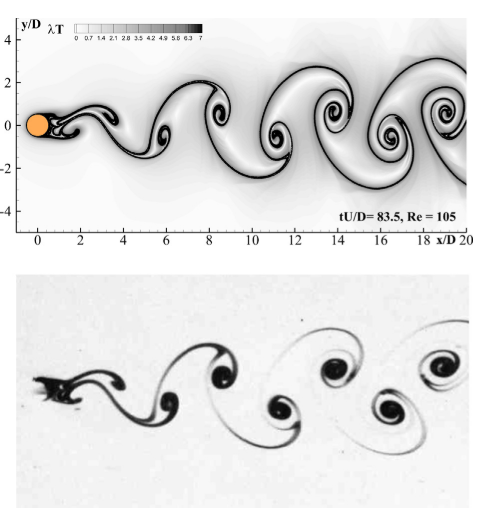
\includegraphics{Figures/research_papers/sun2016detection-fig-1.png}
    \caption{Viscous flow past a circular cylinder at $Re = 105$. Top: Attracting FTLE contour plot from SPH simulation. Bottom: Photo from experiments conducted by \cite{taneda1977visual} with electrolytic precipitation in water technique for vortex street visualisation. Reproduced from \cite{sun2016detection}}
    \label{fig:sun2016detection-fig-1}
\end{figure}

The forward-in-time FTLE is calculated using the forward-in-time Right-Cauchy–Green strain tensor, while backward-in-time FTLE requires the Left-Cauchy–Green strain tensor.
The authors propose two methods to calculate a flow's Cauchy–Green strain tensors.

The first method uses SPH formulations for the deformation gradient to compute the Cauchy–Green strain tensors. The backward-in-time FTLE can be computed using limited resources during run-time concurrently in this method. However, the forward-in-time FTLE can only be computed during post-processing.

In the second method, the forward-in-time deformation gradient is evolved as a property within the simulation's time integration step employing a governing equation for the property. This method does not need to keep track of the spatial relation between the points. This allows for the process to be suitable for Eulerian solvers as well.
Building on this work, \cite{dauch2018highly} developed an efficient GPU-based implementation to accelerate the computation of FTLE fields or, depending on the architecture of the solver, completely move the step from being calculated on the CPU to the GPU. Their proposition is highly enticing, especially for $3D$ flows.

% TODO: More details of Sun2016 required
% Chapter 4

\chapter{Results}
\label{chap:results}

\section{Turbulence-specific Post-processing}

In order to make available, all of the turbulence-specific post-processing from a given simulation output of \texttt{PySPH} \parencite{ramachandran2021a}, generated through the \texttt{Application} class, a \texttt{TurbulentFlowApp} class was created. This class inherits from the \texttt{Application} class and adds additional post-processing attributes and methods, such as:

\begin{itemize}
	\item class attributes:
	\begin{itemize}
		\item number of interpolation points along each axis,
		\item kernel to be used for the interpolation, and the corresponding kernel radius,
		\item interpolation method,
		\item norm order to be used for the computation of the $1D$ energy spectrum (also referred to as the \textit{scalar energy spectrum}),
		\item expected slope for the $1D$ energy spectrum,
        \item type of FTLE field (either \textit{forward} or \textit{backward}),
	\end{itemize}
	
	\item class methods:
	\begin{itemize}
		\item \texttt{compute\_interpolated\_vel\_field}: to compute the interpolated velocity field, at specified indices of the output files,
        \item \texttt{compute\_ek}: to compute the $1D$ energy spectrum from the corresponding interpolated velocity field,
        \item \texttt{compute\_ek\_slope}: to compute the slope of the $1D$ energy spectrum, using the \texttt{scipy.stats.linregress} function,
        \item \texttt{compute\_ftle}: to compute the FTLE (Finite-time Lyapunov Exponent) field, using the corresponding interpolated velocity field between two specific output files,
        \item plotter functions, that can either plot the $1D$ energy spectrum for a specific output file (along with a fit line), or plot the evolution of the $1D$ energy spectrum over a range of output files, or plot the FTLE field.
	\end{itemize}
\end{itemize}

The derived class is also coded to log the details of the interpolator used, which includes details on the kernel, radius scale, problem dimension, SPH equations involved in the interpolation scheme in the original \texttt{problem.log} file created by the default \texttt{Application} class. This enables the user to keep track all of the relevant details of the simulation including its post-processing, in a single log file.

The following subsections, detail the implementation of the energy spectrum and FTLE field computation, and important observations made from the same.


\subsection{Energy Spectral Density}
In order to compute the energy spectrum, the following steps are performed:

\begin{itemize}
    \item the velocity field is interpolated along a grid of uniformly spaced rectangular points,
    \item the velocity field is then transformed to Fourier space, using the \texttt{numpy.fft.fftn} function \parencite{harris2020array}, and subsequently normalised as given as
    \begin{equation}
        \hat{\vect{v_i}}(\vect{k}) = \frac{ fft\{ \vect{v_i}(\vect{r}) \} }{U_0 \times len(\vect{v_i})}
    \end{equation}
    where $U_0$ is a reference velocity and $\vect{v_i}$ is the $i^{th}$ component of the velocity field,
    \item the corresponding energy spectrum is then computed as
    \begin{equation}
        \vect{E_i}(\vect{k}) = \frac{1}{2} \hat{\vect{v_i}}^2
    \end{equation}
    \item the $1D$ energy spectrum $E(k)$ is then computed from the energy vector field $\vect{E_i}(k_x, k_y, k_z)$, by integrating it over the surface of a sphere of appropriate dimension between the limits $k=0$ and $k=k_{max}$, where $k_{max}$ is the maximum wavenumber of the energy spectrum, where 
    \begin{equation}
        k_{max} = round(1 + ceil(|(l_x, l_y, l_z)|/2))
    \end{equation}
\end{itemize}

The function to compute the $1D$ energy spectrum was coded using three different backends, namely, pure \texttt{python}, \texttt{numba} \parencite{Lam_Pitrou_Seibert_2015}, and \texttt{compyle} \parencite{compyle_pr_ab-proc-scipy-2020}.
The speedup results of the three-implementations are shown in \figref{fig:espec-speedup} for $1D$, $2D$, and $3D$ velocity fields respectively.

\begin{figure}[htb!]
    \begin{subfigure}{7cm}
      \centering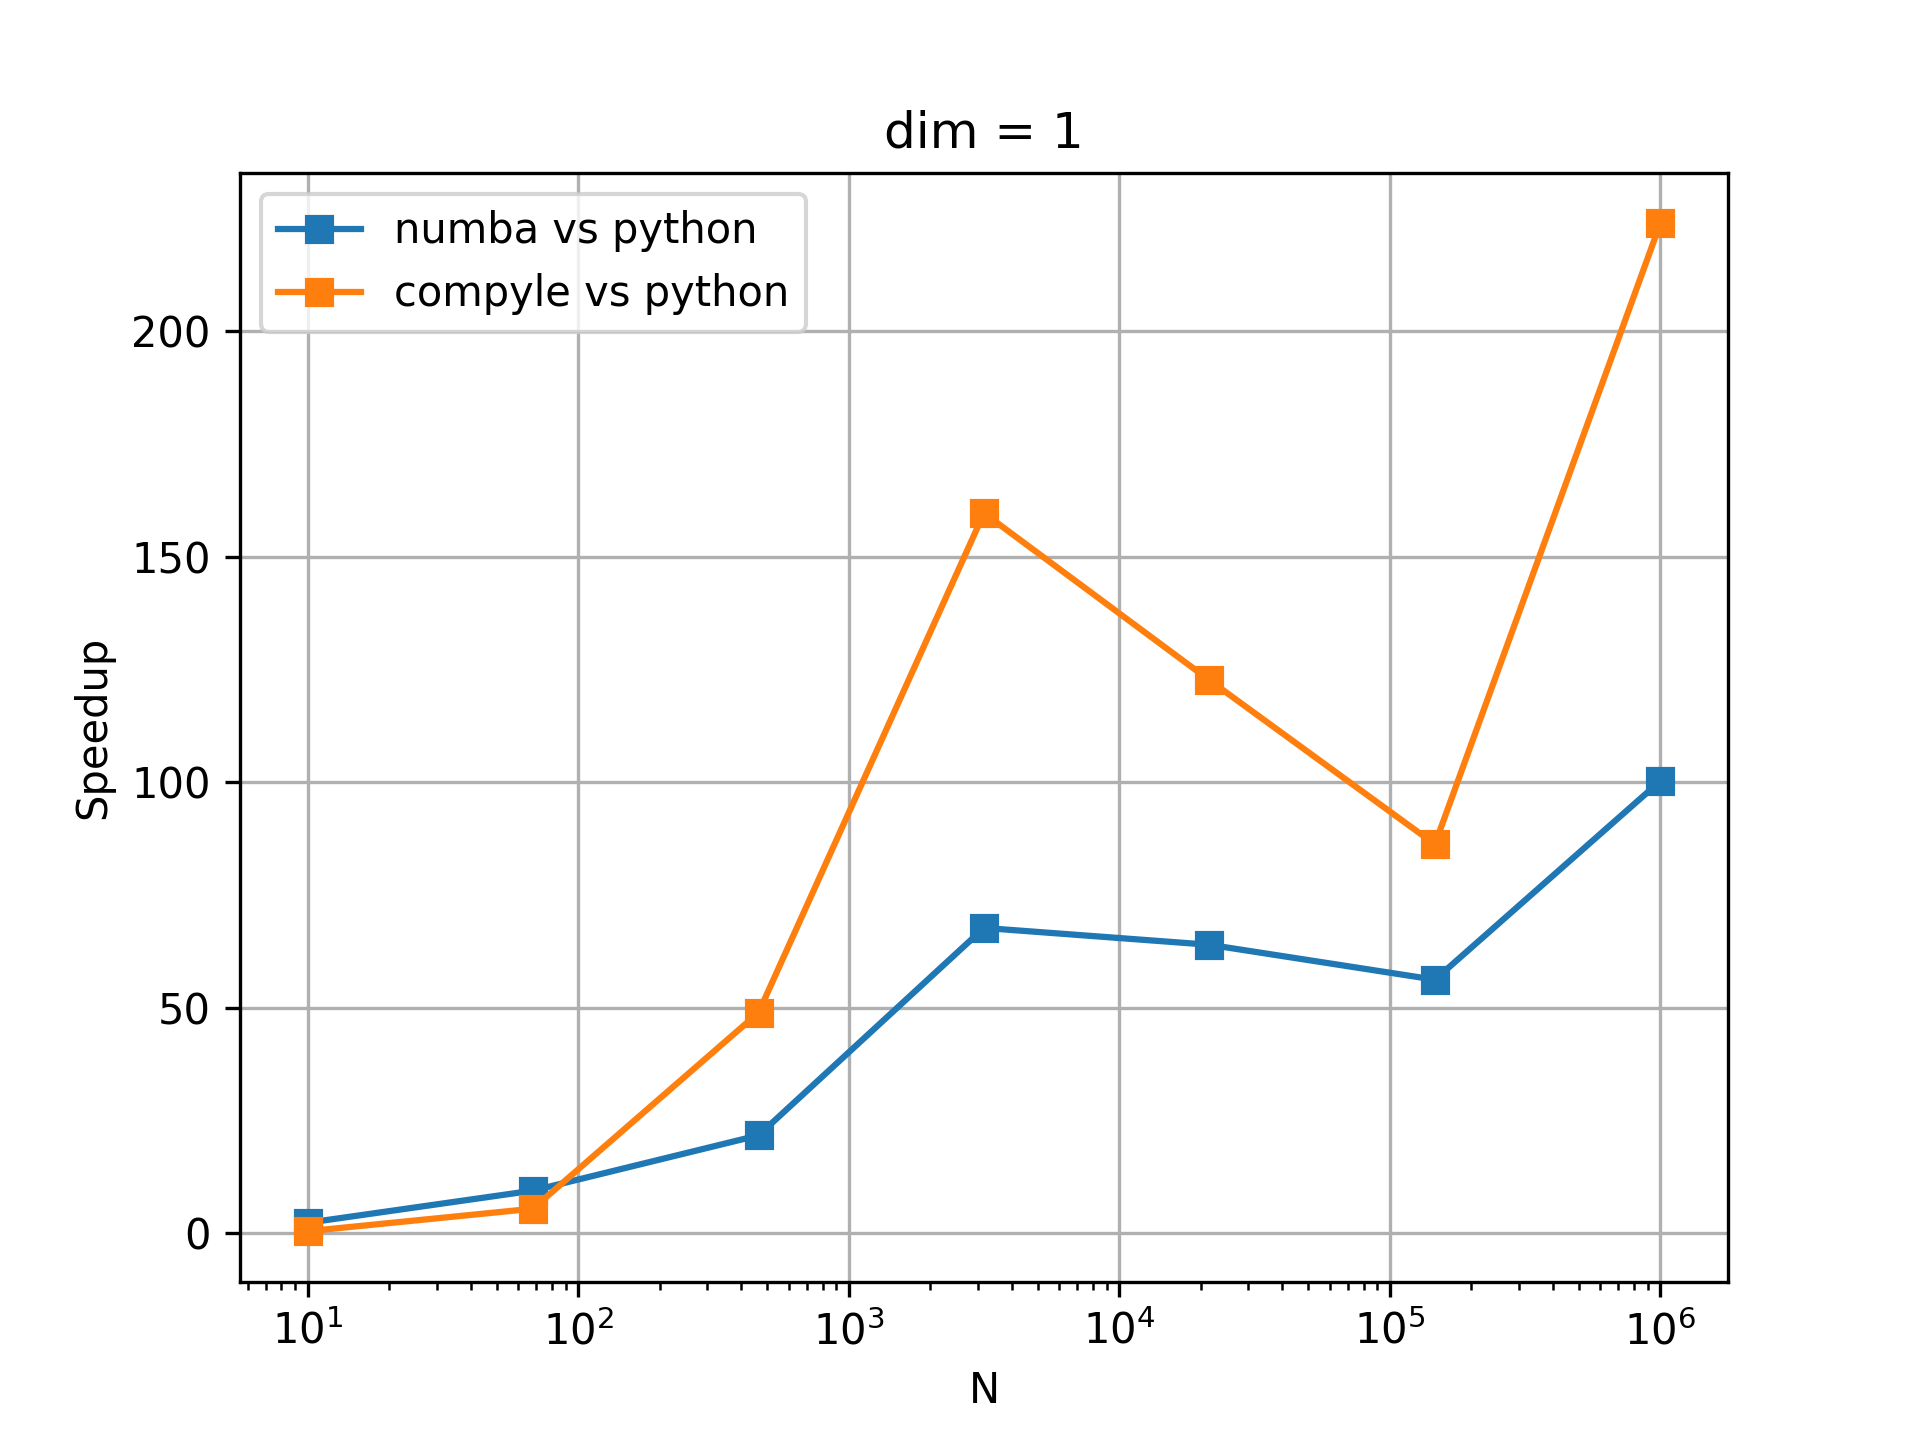
\includegraphics[width=6cm]{Code-Figures/espec_speedup_dim_1.png}
      \caption{$1D$ velocity field}
    \end{subfigure}
    \begin{subfigure}{7cm}
      \centering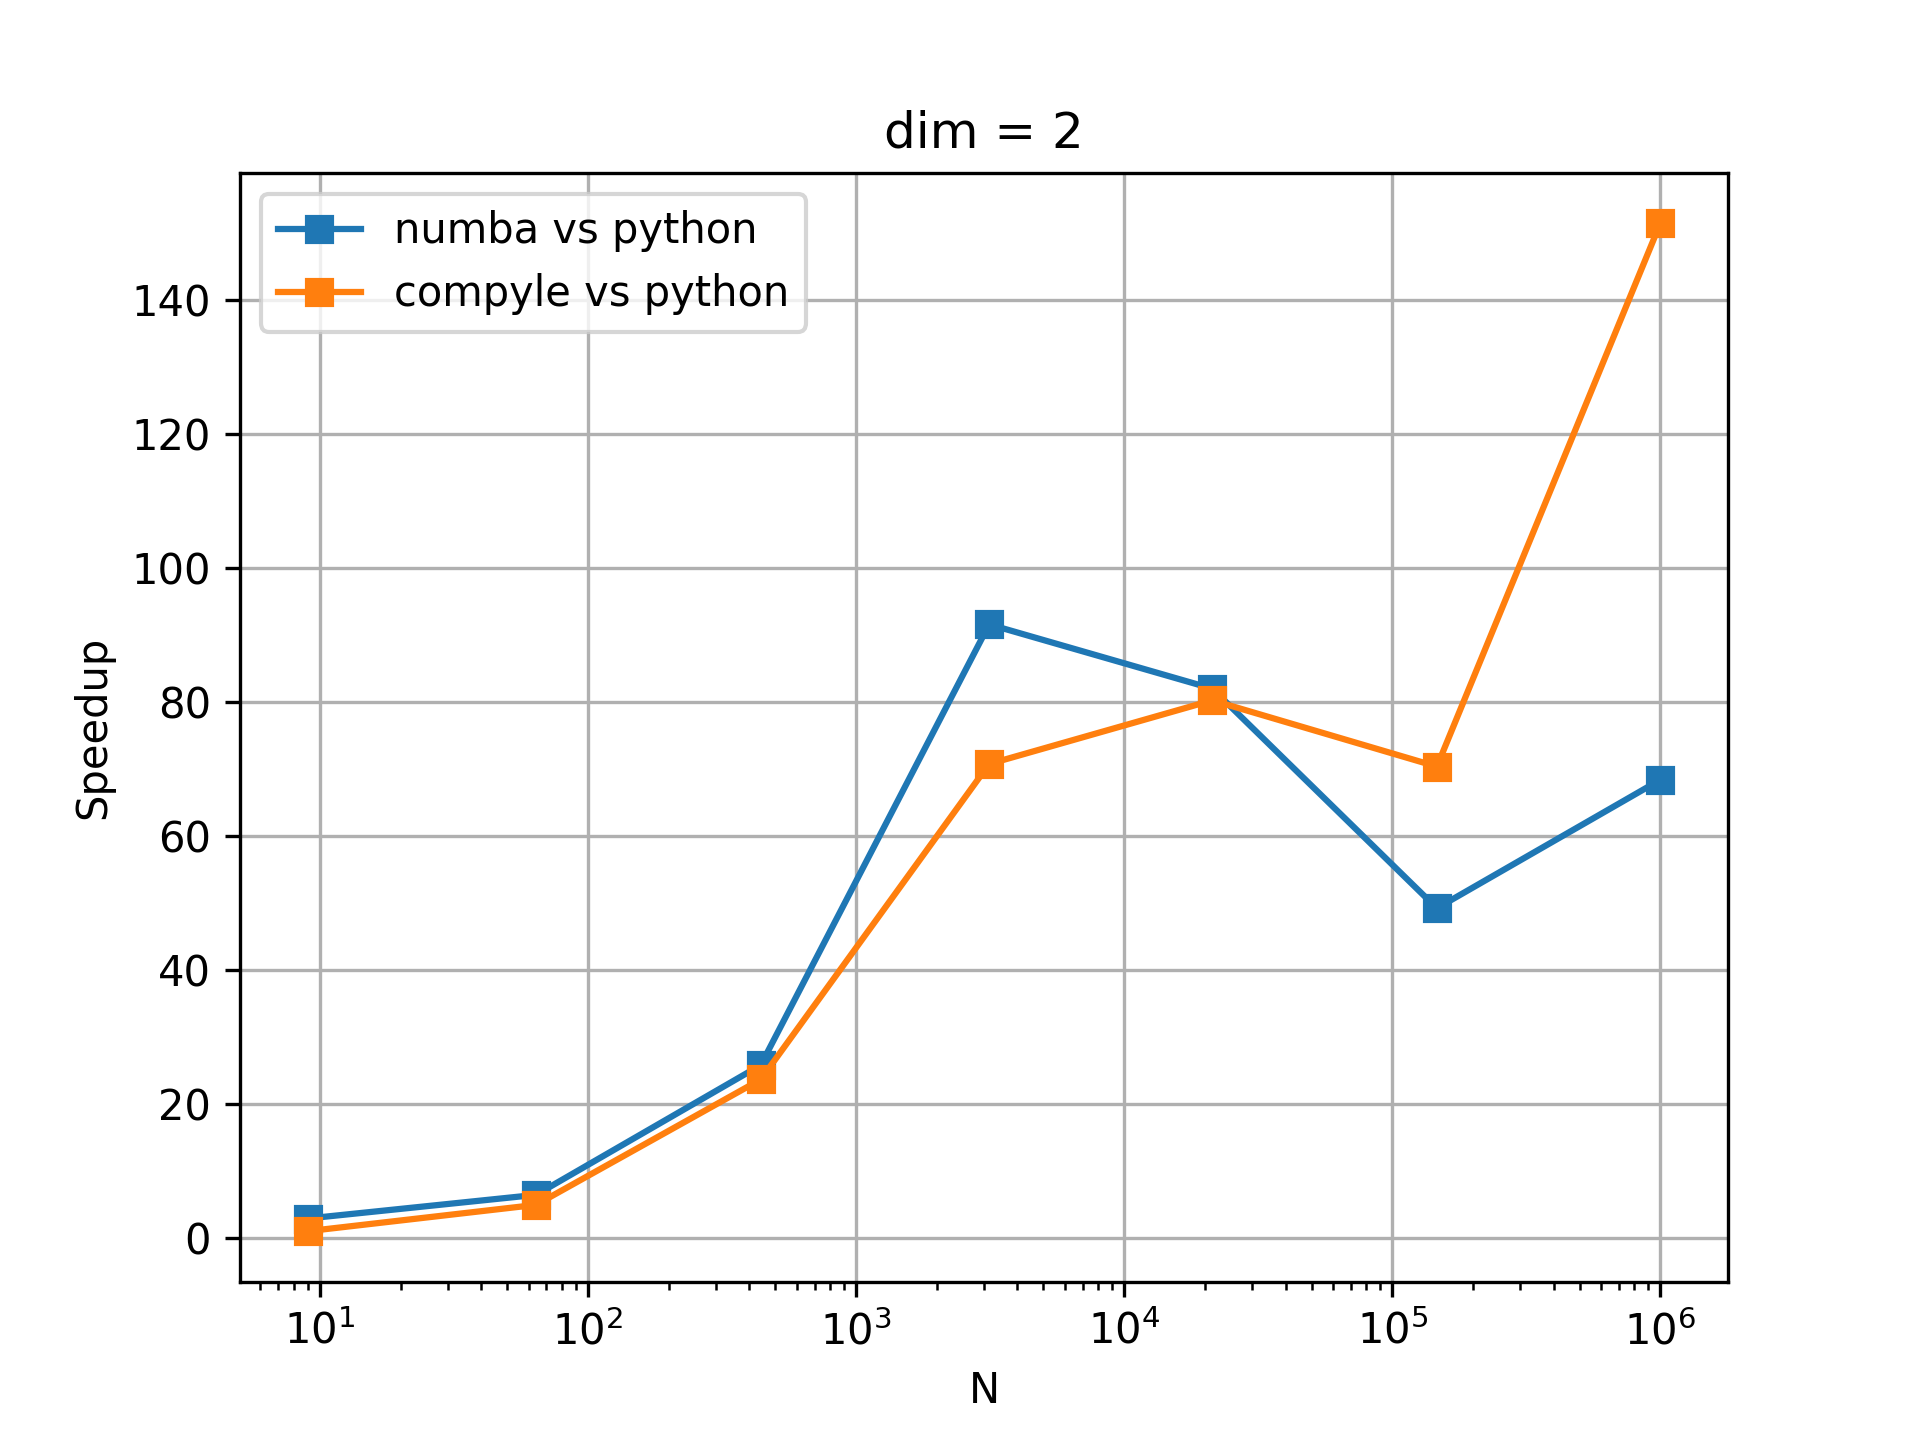
\includegraphics[width=6cm]{Code-Figures/espec_speedup_dim_2.png}
      \caption{$2D$ velocity field}
    \end{subfigure}
    \begin{subfigure}{7cm}
      \centering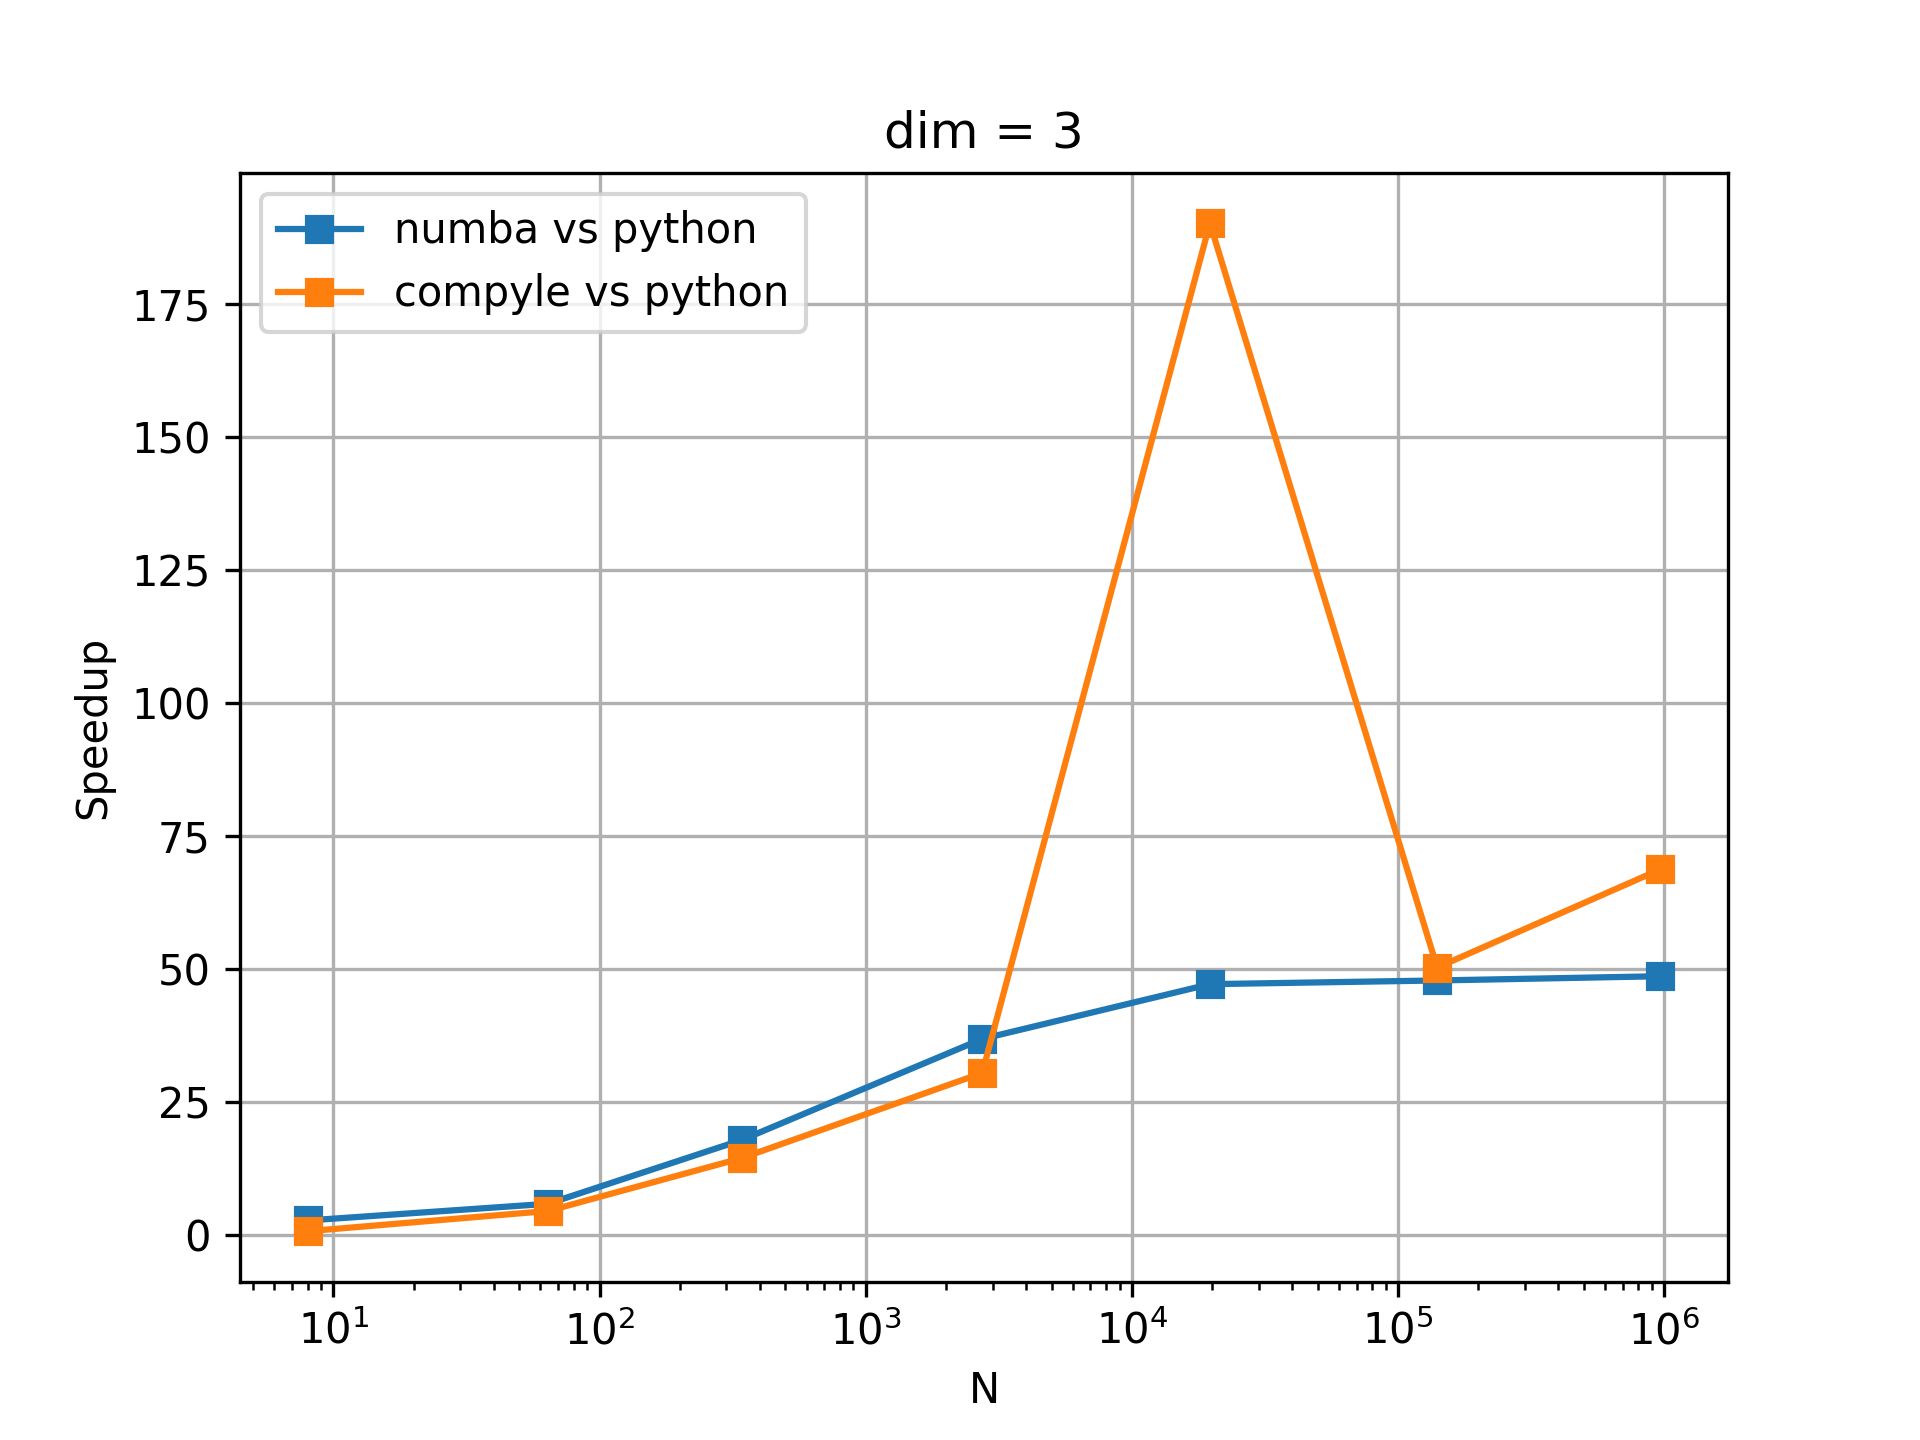
\includegraphics[width=6cm]{Code-Figures/espec_speedup_dim_3.png}
      \caption{$3D$ velocity field}
    \end{subfigure}
    \caption{Speedup of the $1D$ energy spectrum computation for various dimensions of the velocity field.}
    \label{fig:espec-speedup}
\end{figure}

As seen, in the speedup plots, the \texttt{numba} implementation is around $50-100\times$ faster than the pure \texttt{python} implementation, while the \texttt{compyle} implementation is around $80-150\times$ faster than the pure \texttt{python} implementation for various resolution scales. These trends are observed for all the three dimensions of the velocity field. The \texttt{compyle} implementation, in addition to begin faster than the \texttt{numba} implementation, also has the added advantage of not requiring any additional dependencies, which are not already required by \texttt{PySPH}, unlike the \texttt{numba} implementation, which requires the \texttt{numba} package to be installed separately. Hence, the \texttt{compyle} implementation was chosen for the final implementation of the $1D$ energy spectrum computation.

In order to test the code for correctness, the following test-cases were devised. The velocity field for $1D$, is given as:
\begin{equation}
    v_x = - \sum_{i=1}^{N} i^{-\gamma} \cos(2 \pi i x),
\end{equation}
where, $N$ is the number of modes, and $\gamma$ is the decay rate of the modes.
For $2D$, the velocity field is given as:
\begin{equation}
    v_x = - \sum_{i=1}^{N} i^{-\gamma} \cos(2 \pi i x) \sin(2 \pi i y)
\end{equation}
\begin{equation}
    v_y = \sum_{i=1}^{N} i^{-\gamma} \sin(2 \pi i x) \cos(2 \pi i y).
\end{equation}
For $3D$, the velocity field is given as:
\begin{equation}
    v_x = - \sum_{i=1}^{N} i^{-\gamma} \cos(2 \pi i x) \sin(2 \pi i y) \sin(2 \pi i z)
\end{equation}
\begin{equation}
    v_y = \sum_{i=1}^{N} i^{-\gamma} \sin(2 \pi i x) \cos(2 \pi i y) \sin(2 \pi i z)
\end{equation}
\begin{equation}
    v_z = \sum_{i=1}^{N} i^{-\gamma} \sin(2 \pi i x) \sin(2 \pi i y) \cos(2 \pi i z).
\end{equation}
Since the energy in the flow field is a function of the square of the velocity, the corresponding decay rate in the energy spectrum is going to be $2\gamma$.

First order of correctness, involved running the energy spectral calculation for the above test-cases, using only one mode ($N=1$), and zero decay rate ($\gamma=0$).

The vector energy spectral fields are show in \figref{fig:espec-vector-fields-N1}. It should be noted, that the plots are shown by shifting the energy spectrum, such that the center of the plot corresponds to the zero wavenumber. This is done, since the energy spectrum is symmetric about the zero wavenumber, and hence, the plot is more informative when the zero wavenumber is at the center of the plot. Here, it can be observed that in both the $1D$ and $2D$ case the energy spectrum peaks only for $k=1$, and is zero for every other wavenumber, indicating the nature of the velocity field, consisting of only one mode. 

The scalar energy spectral fields are shown in \figref{fig:espec-scalar-fields-N1}. As can be seen, the energy spectrum peaks only for $k=1$, and is zero for every other wavenumber for all dimensions.

\begin{figure}[htb!]
    \begin{subfigure}{7cm}
      \centering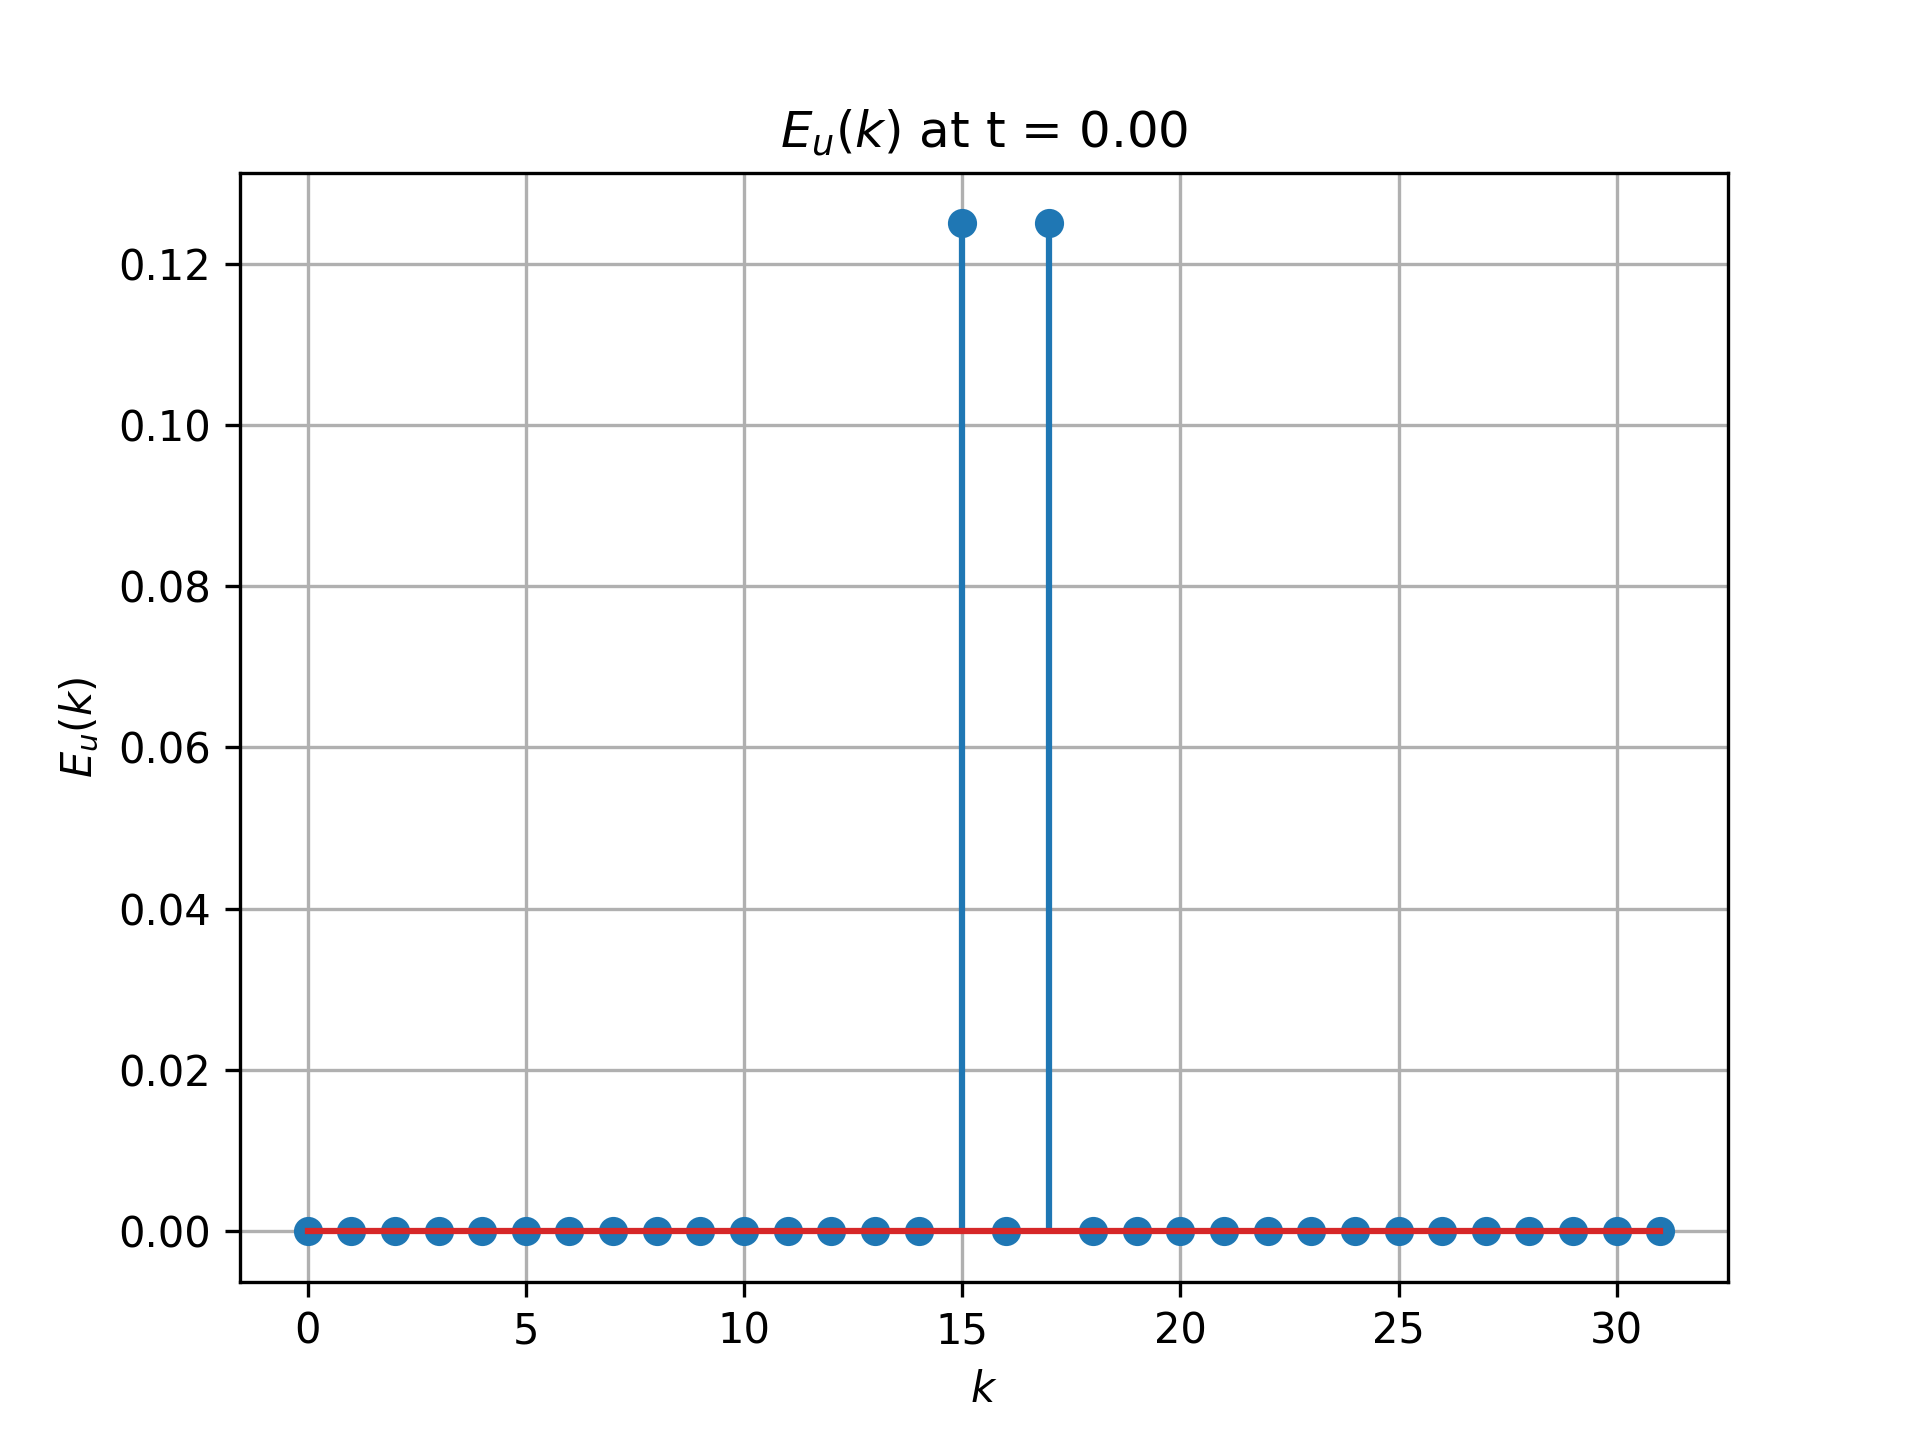
\includegraphics[width=6cm]{Code-Figures/espec-simple-1d/EK_spectrum.png}
      \caption{$1D$ $\vect{E}(\vect{k})$ field}
    \end{subfigure}
    \begin{subfigure}{7cm}
      \centering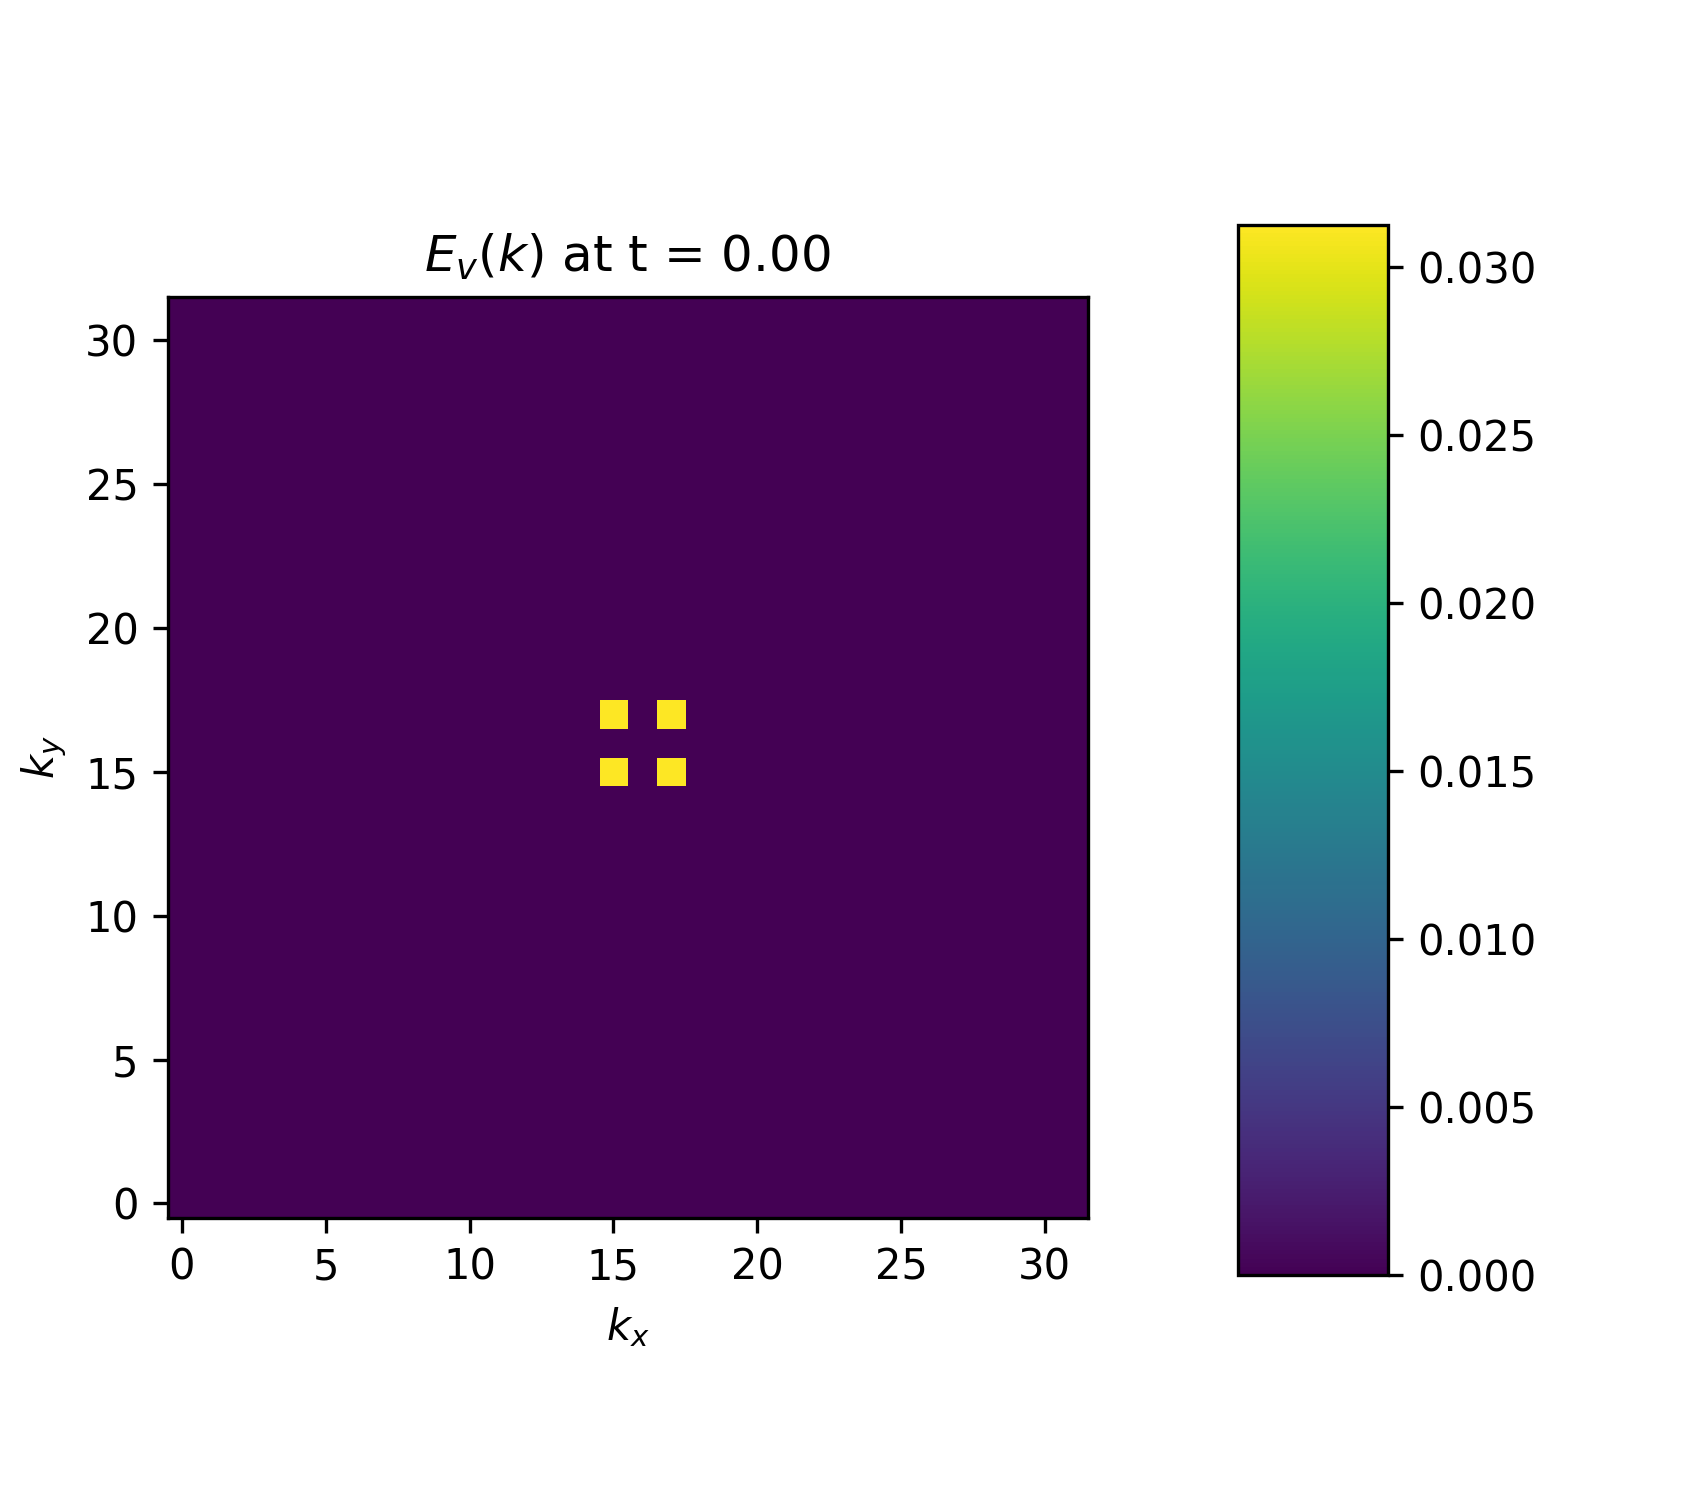
\includegraphics[width=6cm]{Code-Figures/espec-simple-2d/EK_spectrum.png}
      \caption{$2D$ $\vect{E}(\vect{k})$ field}
    \end{subfigure}
    \caption{The vector fields $\vect{E}(\vect{k})$ for $1D$ and $2D$ case, with decay rate $\gamma=0$, and $N=1$.}
    \label{fig:espec-vector-fields-N1}
\end{figure}

\begin{figure}[htb!]
    \begin{subfigure}{7cm}
      \centering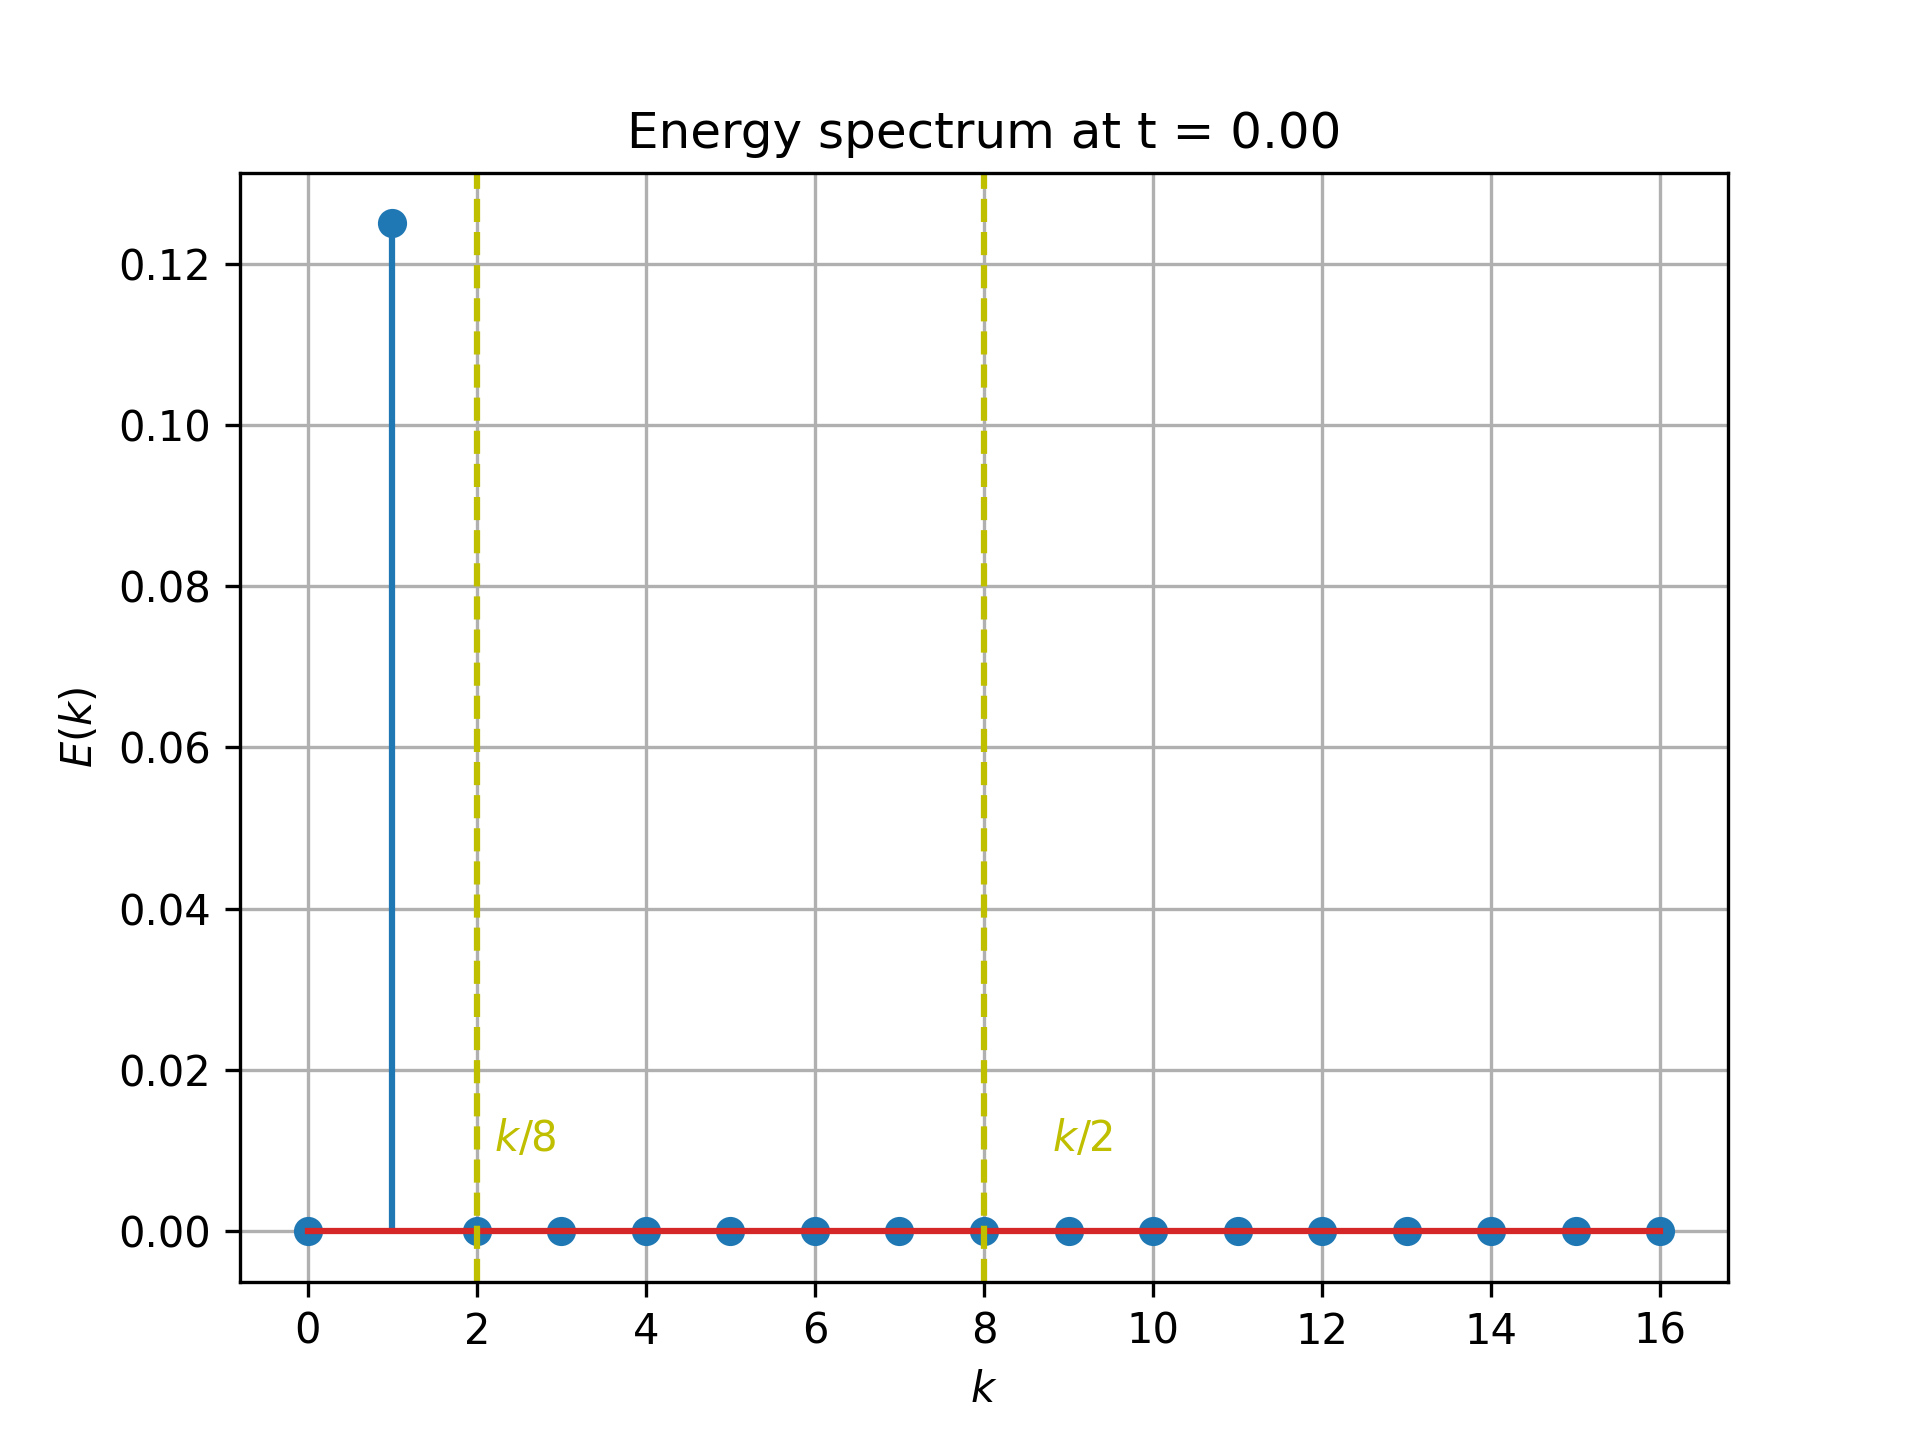
\includegraphics[width=6cm]{Code-Figures/espec-simple-1d/energy_spectrum.png}
      \caption{$1D$ $E(k)$ field}
    \end{subfigure}
    \begin{subfigure}{7cm}
      \centering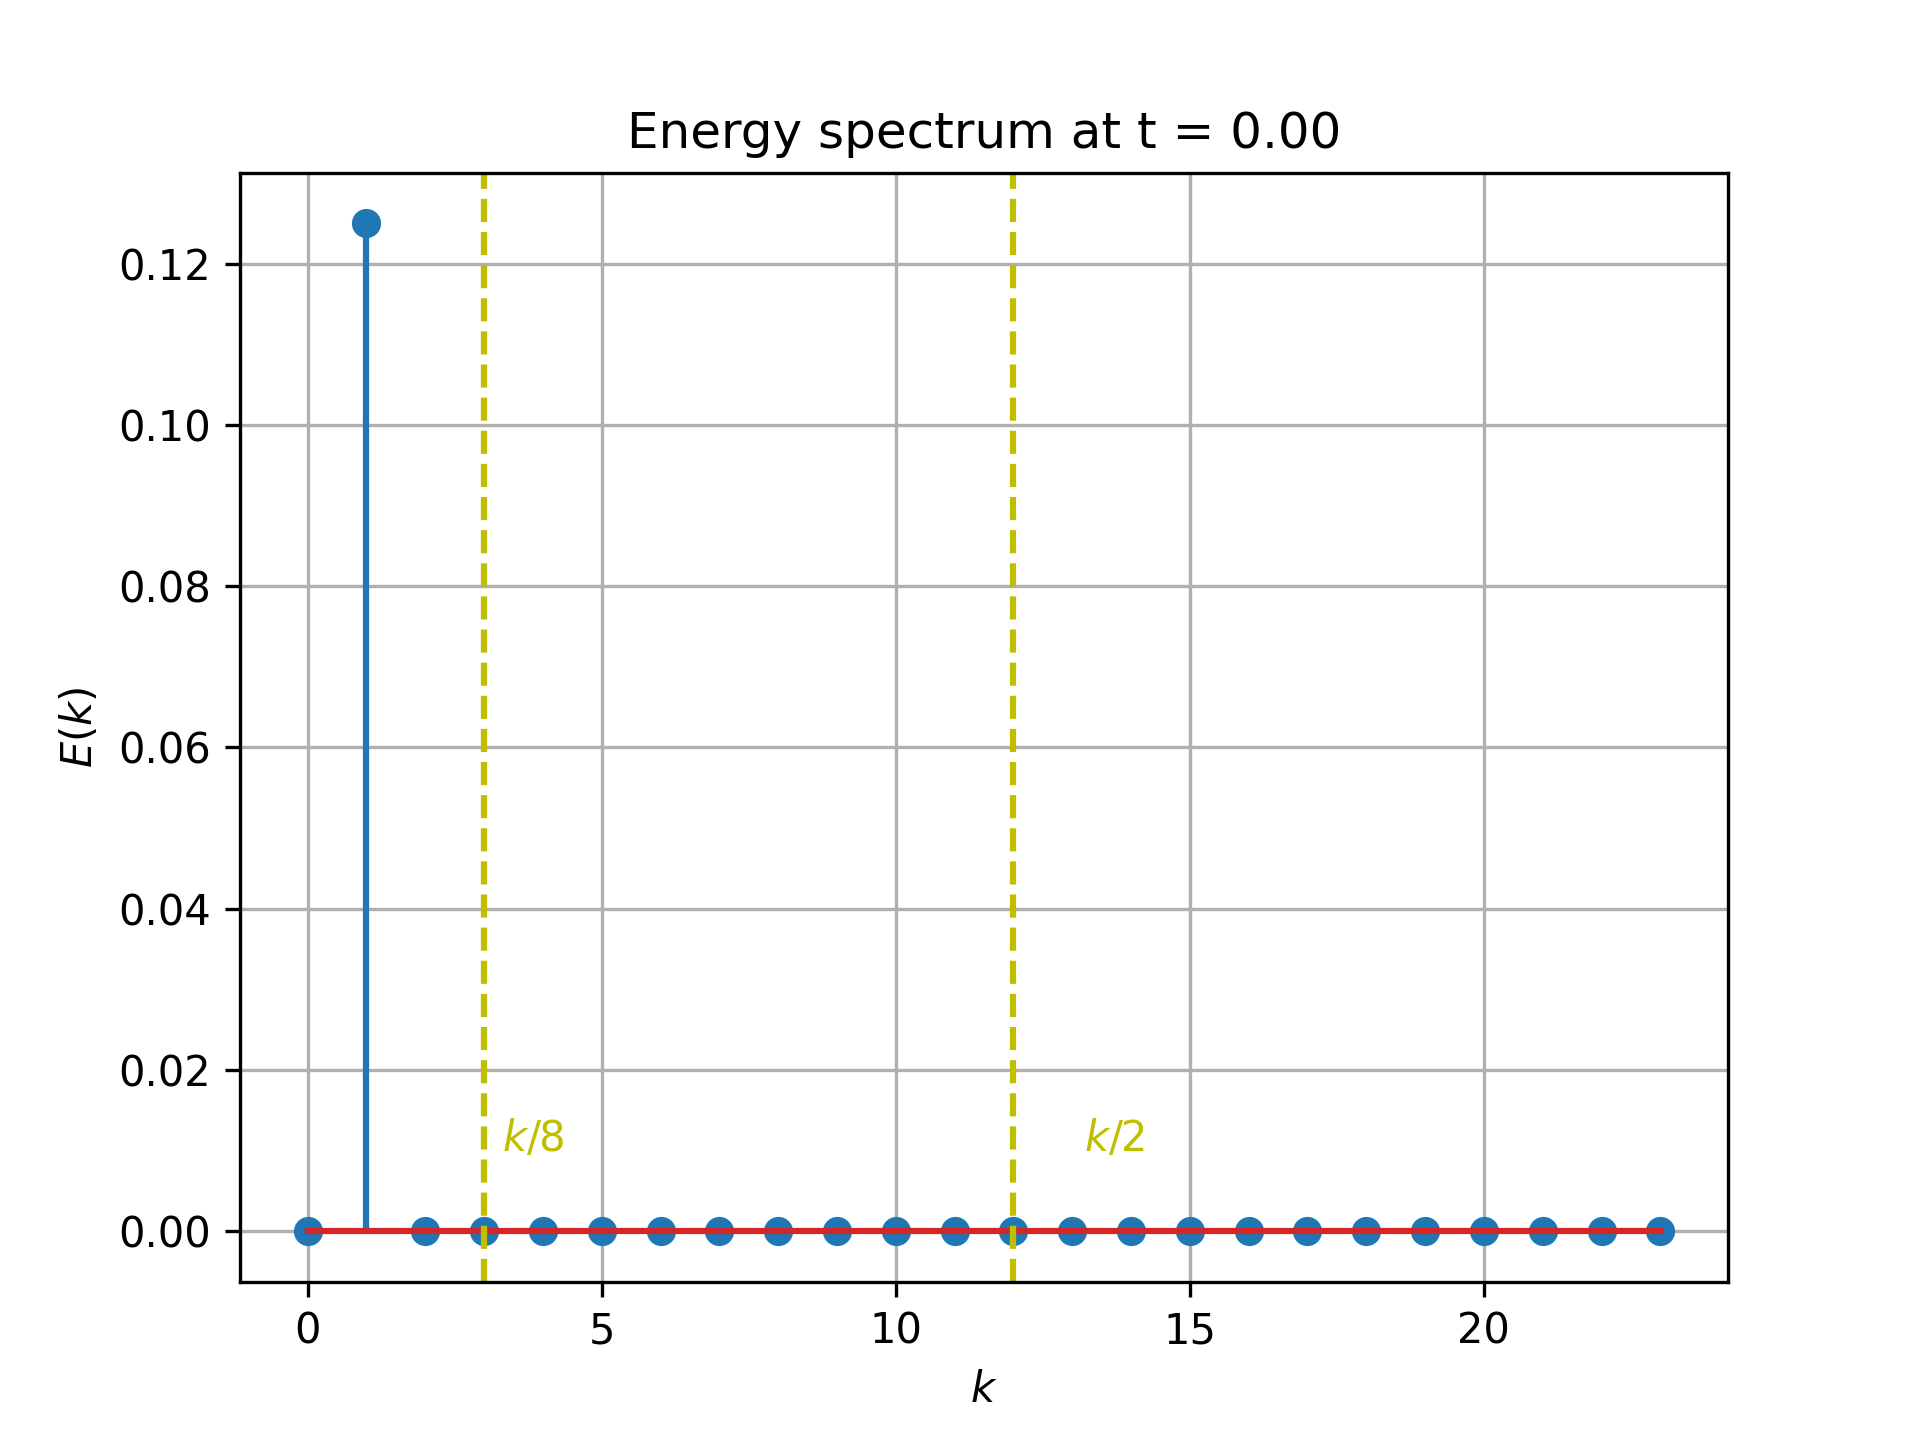
\includegraphics[width=6cm]{Code-Figures/espec-simple-2d/energy_spectrum.png}
      \caption{$2D$ $E(k)$ field}
    \end{subfigure}
    \begin{subfigure}{7cm}
        \centering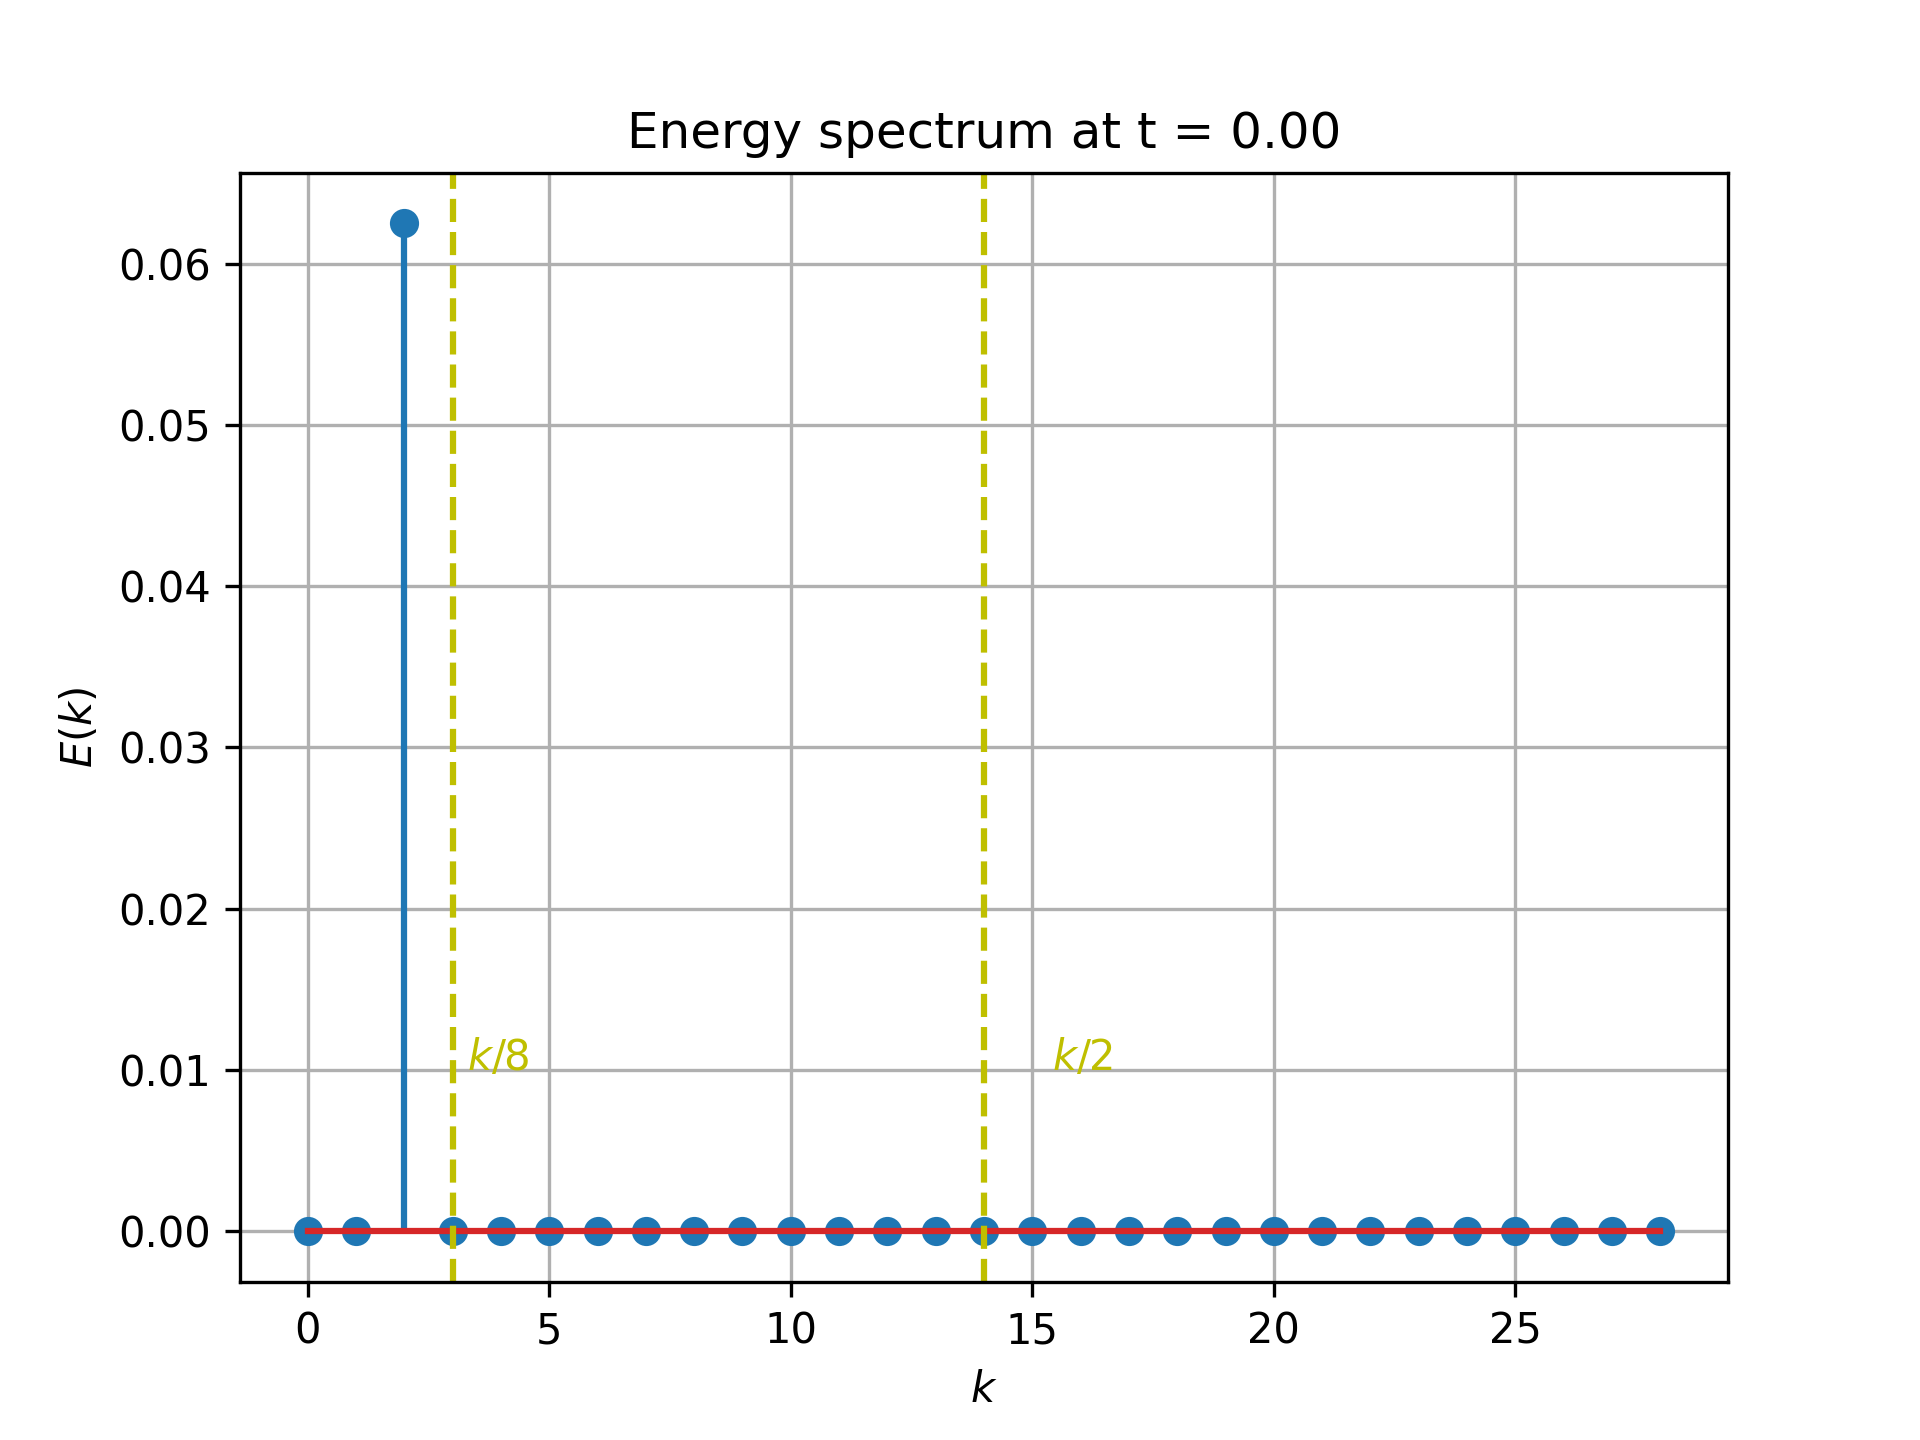
\includegraphics[width=6cm]{Code-Figures/espec-simple-3d/energy_spectrum.png}
        \caption{$3D$ $E(k)$ field}
      \end{subfigure}
    \caption{The scalar fields $E(k)$ for $1D$, $2D$, and $3D$ case, with decay rate $\gamma=0$, and $N=1$.}
    \label{fig:espec-scalar-fields-N1}
\end{figure}

Subsequently, to test the correctness when multiple modes are involved, the test-cases were reconsidered, with $\gamma=1$, and $N$ equal to half the number of particles along one axis of the problem.

The vector energy spectral fields are show in \figref{fig:espec-vector-fields-gamma1}. Here, it can be observed that in both the $1D$ and $2D$ case the energy spectrum peaks for $k=1$, and is non-zero upto $k=n_x/2$, indicating the nature of the velocity field, consisting of multiple modes. The amplitudes are also observed to have an exponential drop-off, as is expected given the nature of the amplitude weigthing.

This is made all the more clear, with the scalar energy spectral fields shown in \figref{fig:espec-scalar-fields-gamma1}. The log-log plots here, allow for the exponential drop-off to be observed more clearly, by fitting a straight line to the log-log plot between wavenumbers $k \in [1, n_x/4]$. The gree-dashed lines which represent the scalar energy spectrum computed for the original velocity field (which is uniform, and rectangular) without interpolation, represents the `best'-case scenario, where the energy spectrum is computed without any loss of information in the velocity field, and the source of noise can be solely attributed to numerical errors from the discrete Fourier transform. The actual scalar energy spectrum computed from the interpolated velocity is plotted in blue.

It is oberseved that energy spectrum computed without interpolation, is indeed the `best'-case scenario, since it much more closely follows the exact trend. However, with the computed energy spectrum from the interpolated velocity field, the trend is still observed to be followed, but only upto the $k/8$ wavenumber, beyond which the trend is lost, and the computed energy spectrum is observed to be much lower than the green-dashed line, with the difference increasing with the wavenumber.
This seems to indicate that the act of interpolation itself, is introducing some amount of noise in the velocity field, which is reflected by the jagged nature of the blue line, and also seems to decrease the energy at lower scales, which is reflected by the blue line being consistently lower than the green-dashed line at lower wavenumbers. This allows for the conclusion that the interpolation scheme, seems to behave as a low-pass filter, which is expected, since the interpolation scheme is essentially a convolution of the velocity field with the kernel function, which is a low-pass filter.

Therefore, it was concluded that the $1D$ energy field, computed from the interpolated velocity field, typically will underestimate the energy at higher wavenumbers, and hence, the slope of the energy spectrum computed from the interpolated velocity field, will be lower than the slope of the energy spectrum computed from the original velocity field, as reflected in \figref{fig:espec-scalar-fields-gamma1} as well.

\begin{figure}[htb!]
    \begin{subfigure}{7cm}
      \centering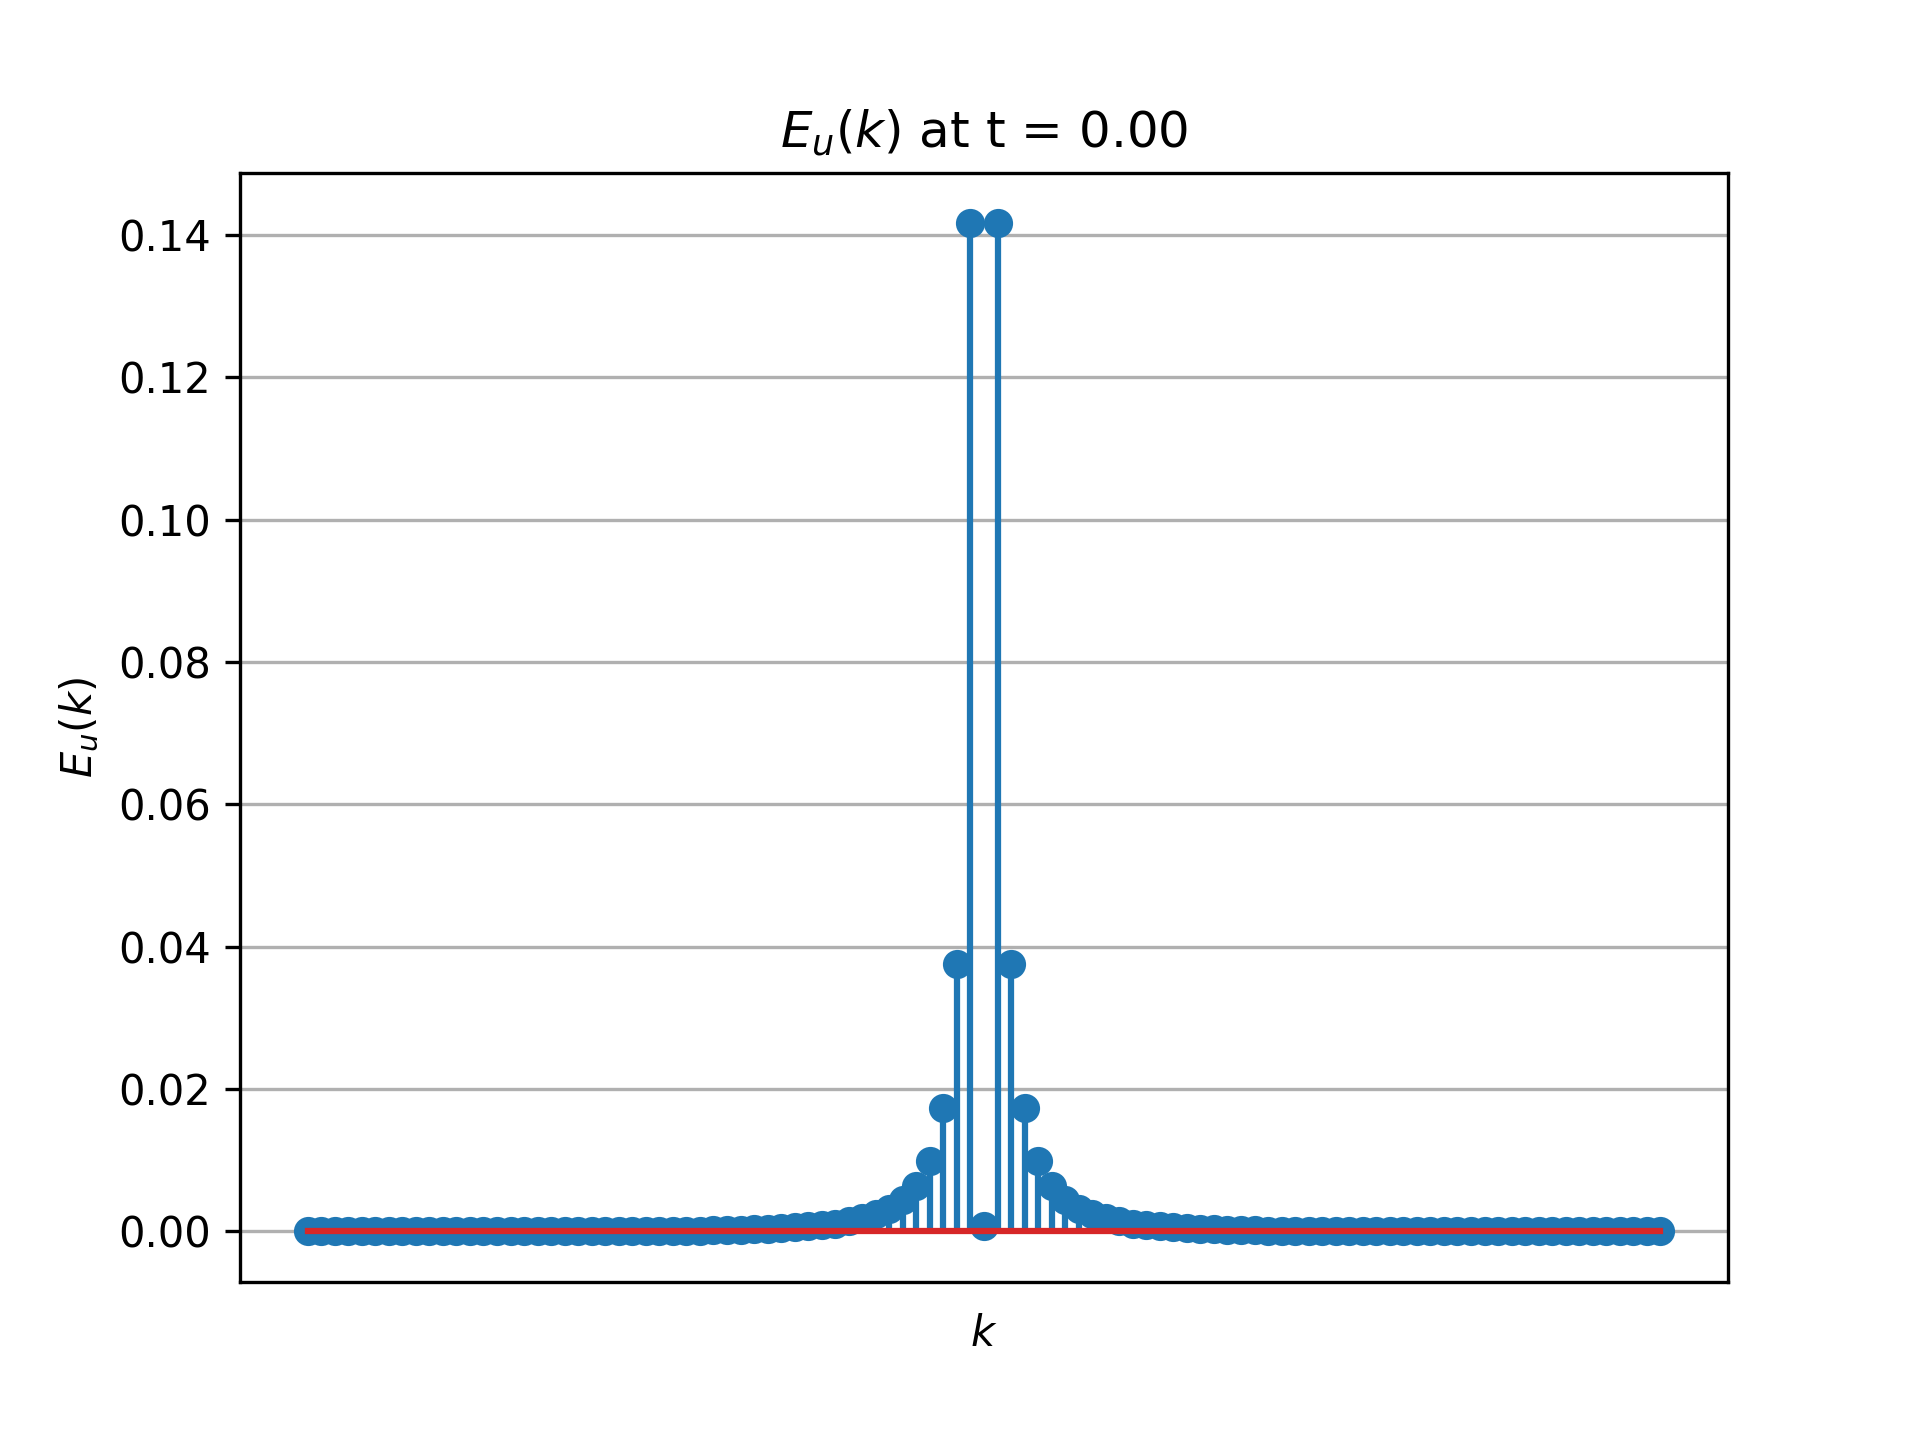
\includegraphics[width=6cm]{Code-Figures/sine-vel-prof-1d/EK_spectrum.png}
      \caption{$1D$ $\vect{E}(\vect{k})$ field}
    \end{subfigure}
    \begin{subfigure}{7cm}
      \centering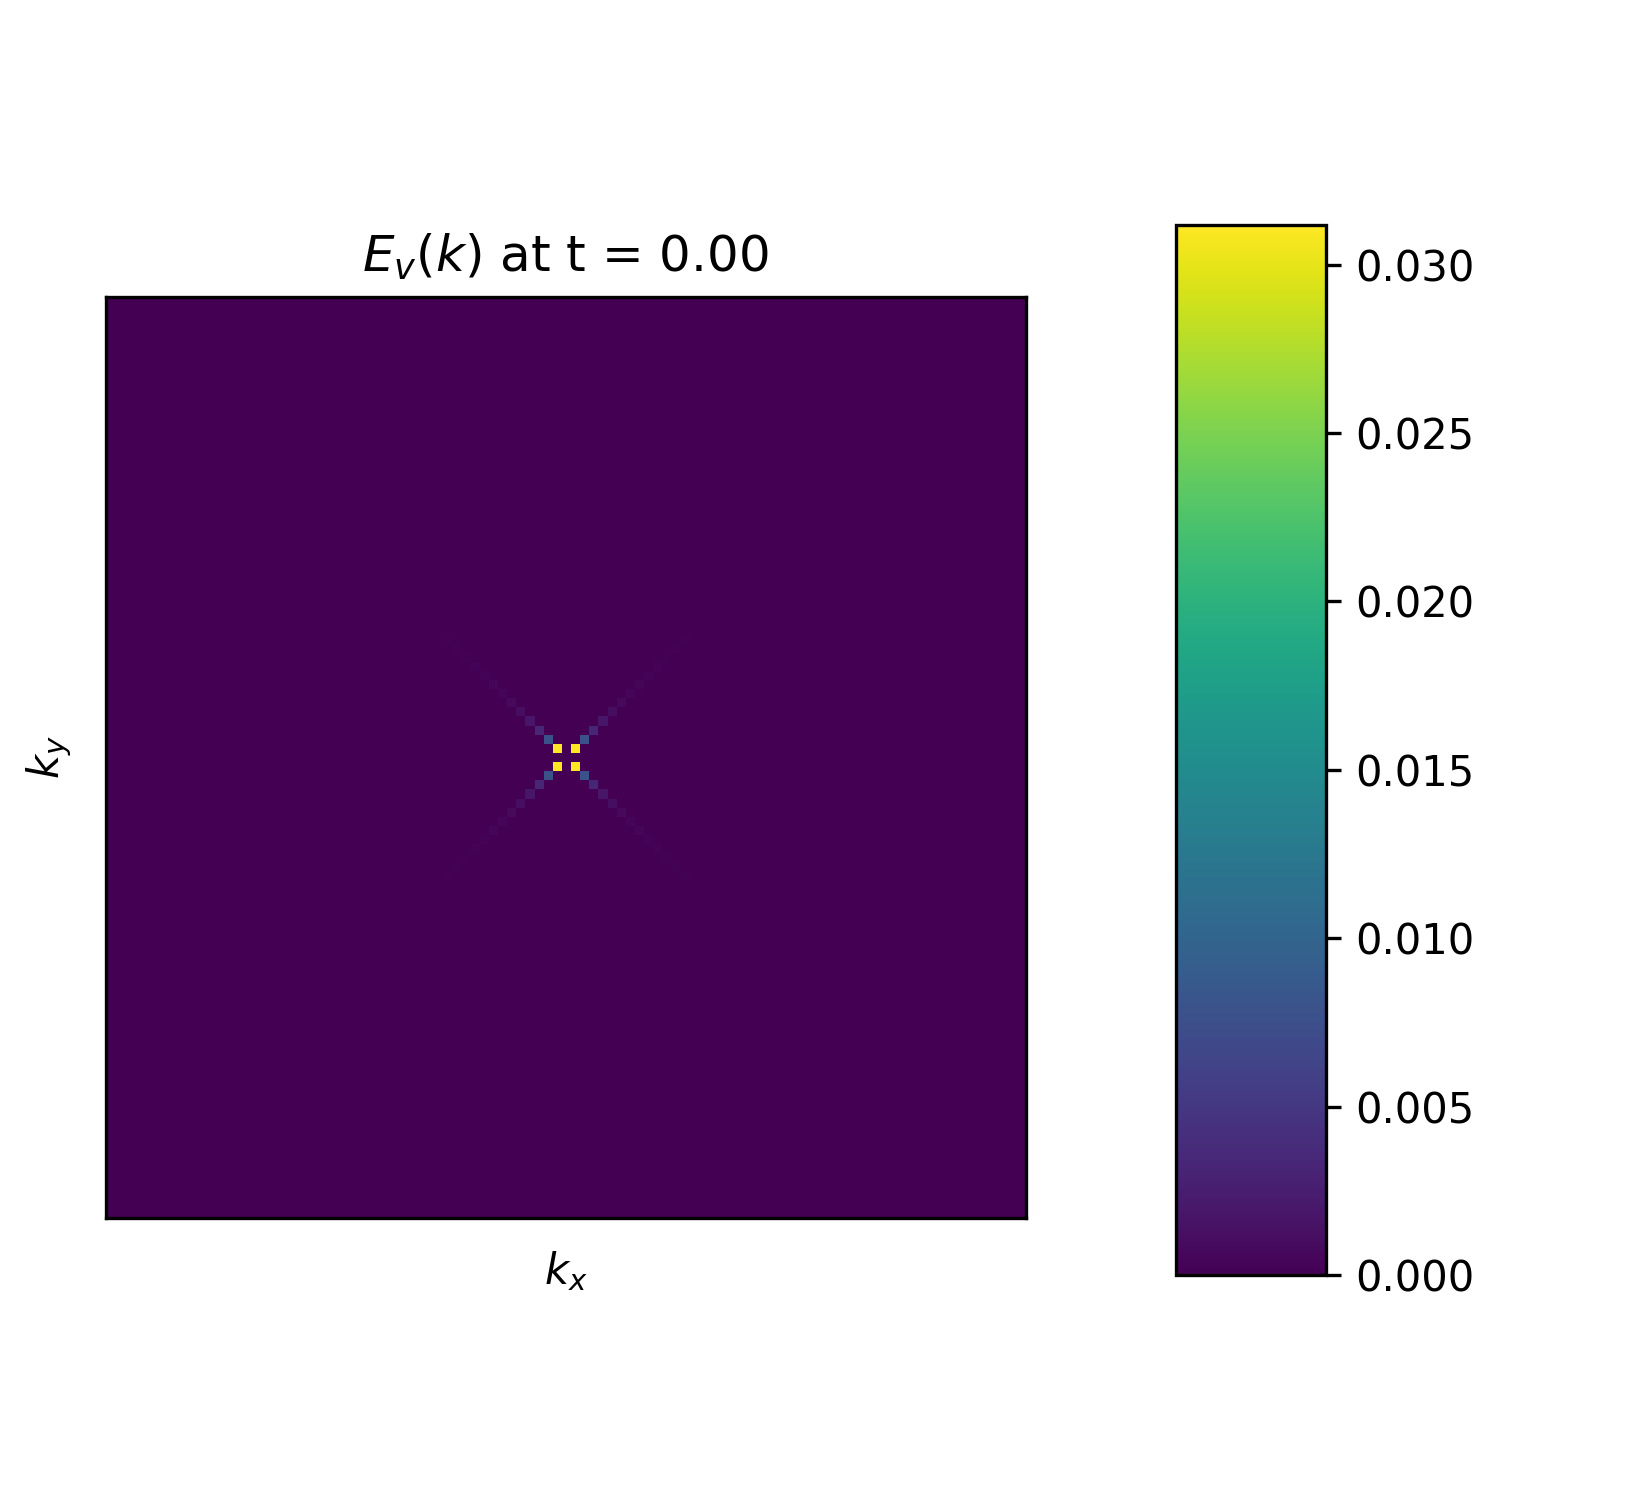
\includegraphics[width=6cm]{Code-Figures/sine-vel-prof-2d/EK_spectrum.png}
      \caption{$2D$ $\vect{E}(\vect{k})$ field}
    \end{subfigure}
    \caption{The vector fields $\vect{E}(\vect{k})$ for $1D$ and $2D$ case, with decay rate $\gamma=1$, and $N=n_x/2$.}
    \label{fig:espec-vector-fields-gamma1}
\end{figure}

\begin{figure}[htb!]
    \begin{subfigure}{7cm}
      \centering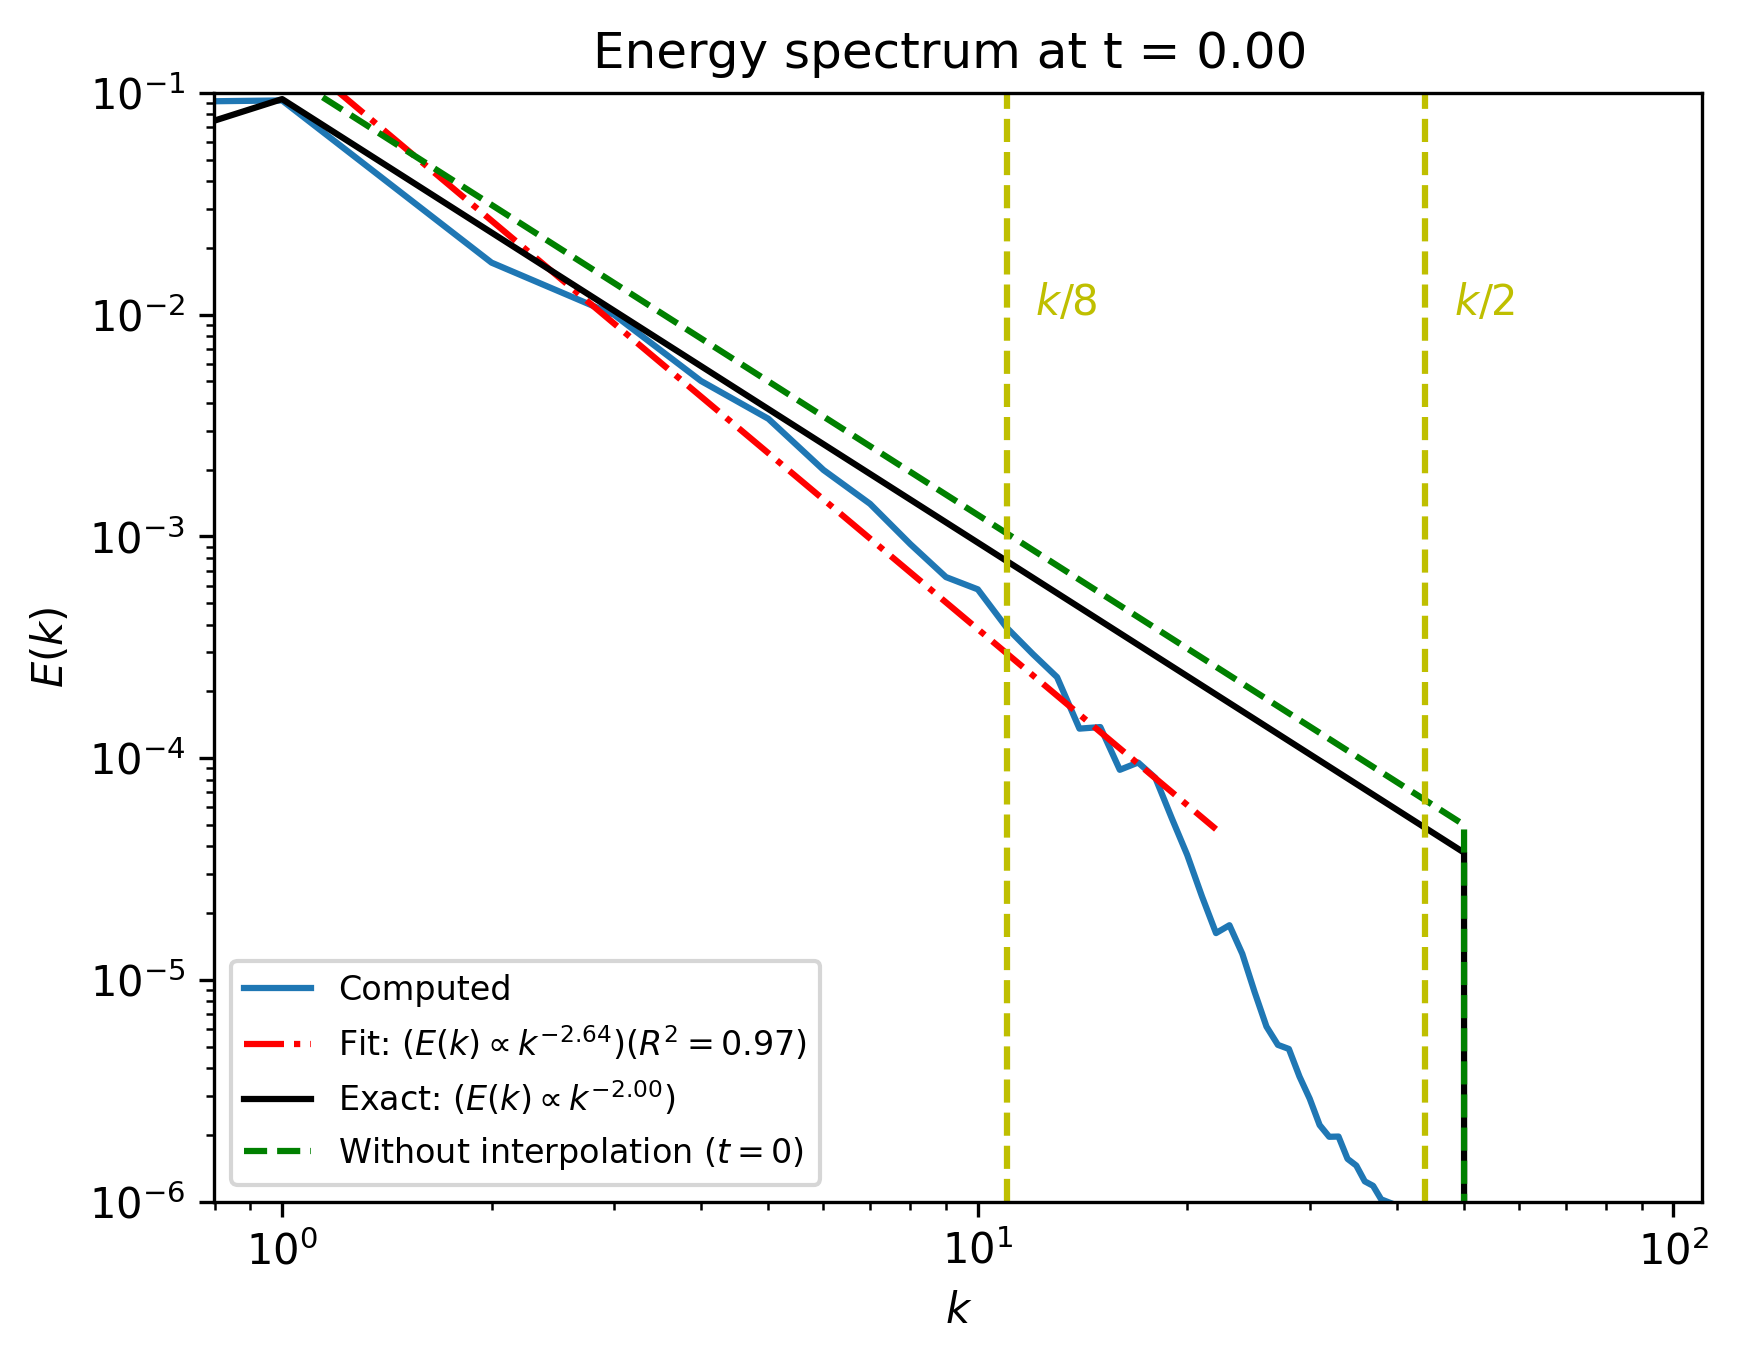
\includegraphics[width=6cm]{Code-Figures/sine-vel-prof-1d/ek_00000_loglog.png}
      \caption{$1D$ $E(k)$ field}
    \end{subfigure}
    \begin{subfigure}{7cm}
      \centering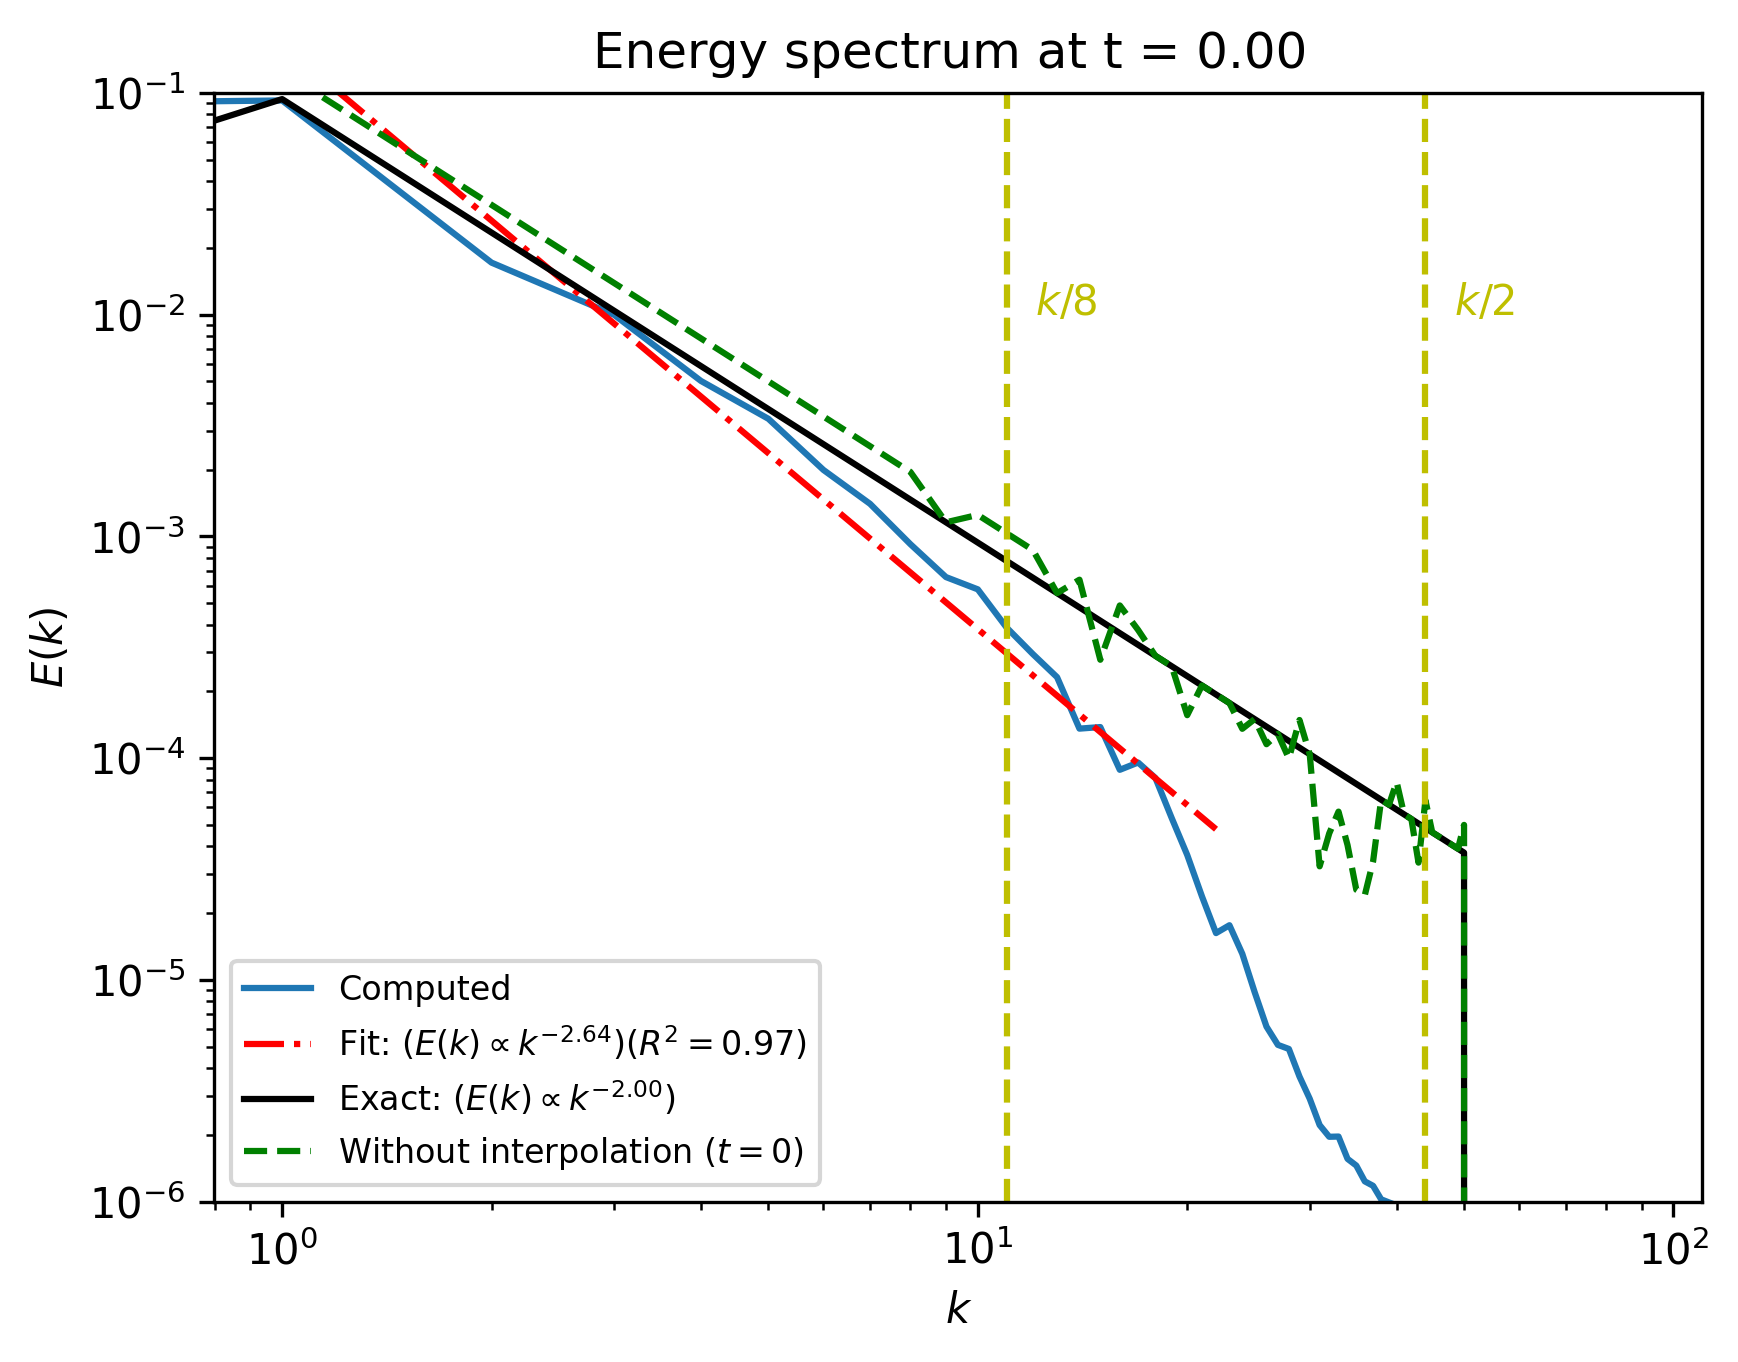
\includegraphics[width=6cm]{Code-Figures/sine-vel-prof-2d/ek_00000_loglog.png}
      \caption{$2D$ $E(k)$ field}
    \end{subfigure}
    \begin{subfigure}{7cm}
        \centering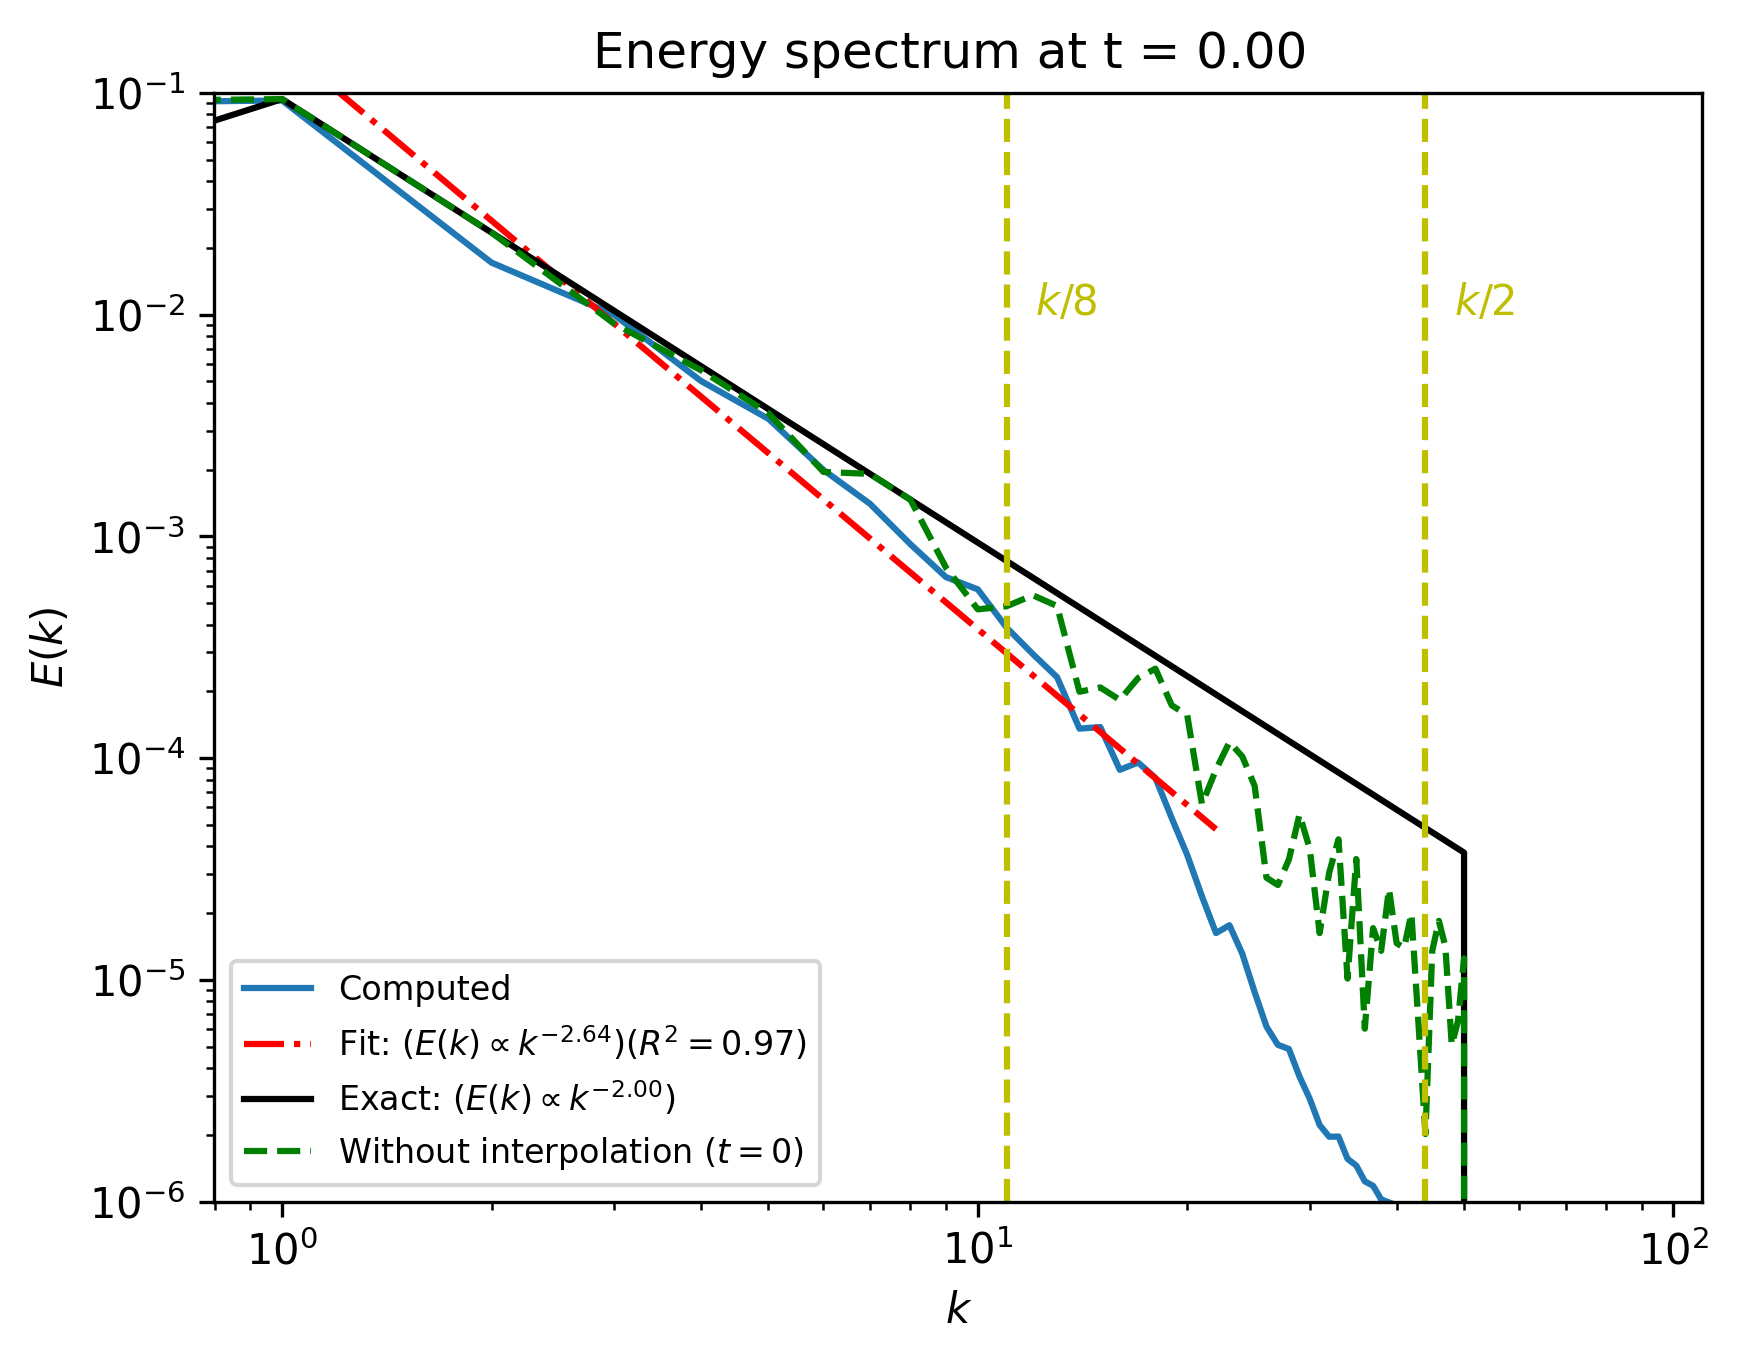
\includegraphics[width=6cm]{Code-Figures/sine-vel-prof-3d/ek_00000_loglog.png}
        \caption{$3D$ $E(k)$ field}
      \end{subfigure}
    \caption{The scalar fields $E(k)$ for $1D$, $2D$, and $3D$ case, with decay rate $\gamma=1$, and $N=n_x/2$.}
    \label{fig:espec-scalar-fields-gamma1}
\end{figure}

The same set of test-cases, with $\gamma=1$ and $N=n_x/2$, are considered, in order to identify the effect of various interpolation schemes, kernels, perturbation, and resolutions on the computed energy spectrum.

In order to measure the effect of the perturbation in the particle spacing on the computed energy spectrum, once a rectangluar grid of uniform particles are defined, its coordinates are perturbed by a uniform random number $\delta \hat{x} \in [0, 1)$, scaled by a perturbation amplitude. The perturbed grid is then initialised with the corresponding velocity profile, and the energy spectrum is computed for the perturbed grid. From the results shown in \figref{fig:espec-scalar-fields-per-ampl}, it can be observed that by increasing the perturbation amplitude, energy seems to be introduced at lower resolution scales, which is reflected by the icreased energy at higher wavenumbers. This trend seems to hold true, for all dimensions.
Therefore, we can infer that the low-pass energy dissipation effect of the interpolation scheme, will to an extent be countered by the perturbation in the particle spacing (which is typically the case in a simulation since the particles become disturbed), which will introduce energy at lower resolution scales, and hence, the slope of the energy spectrum computed from the interpolated velocity field, will be closer to the slope of the energy spectrum computed from the original velocity field. 

\begin{figure}[htb!]
    \begin{subfigure}{7cm}
      \centering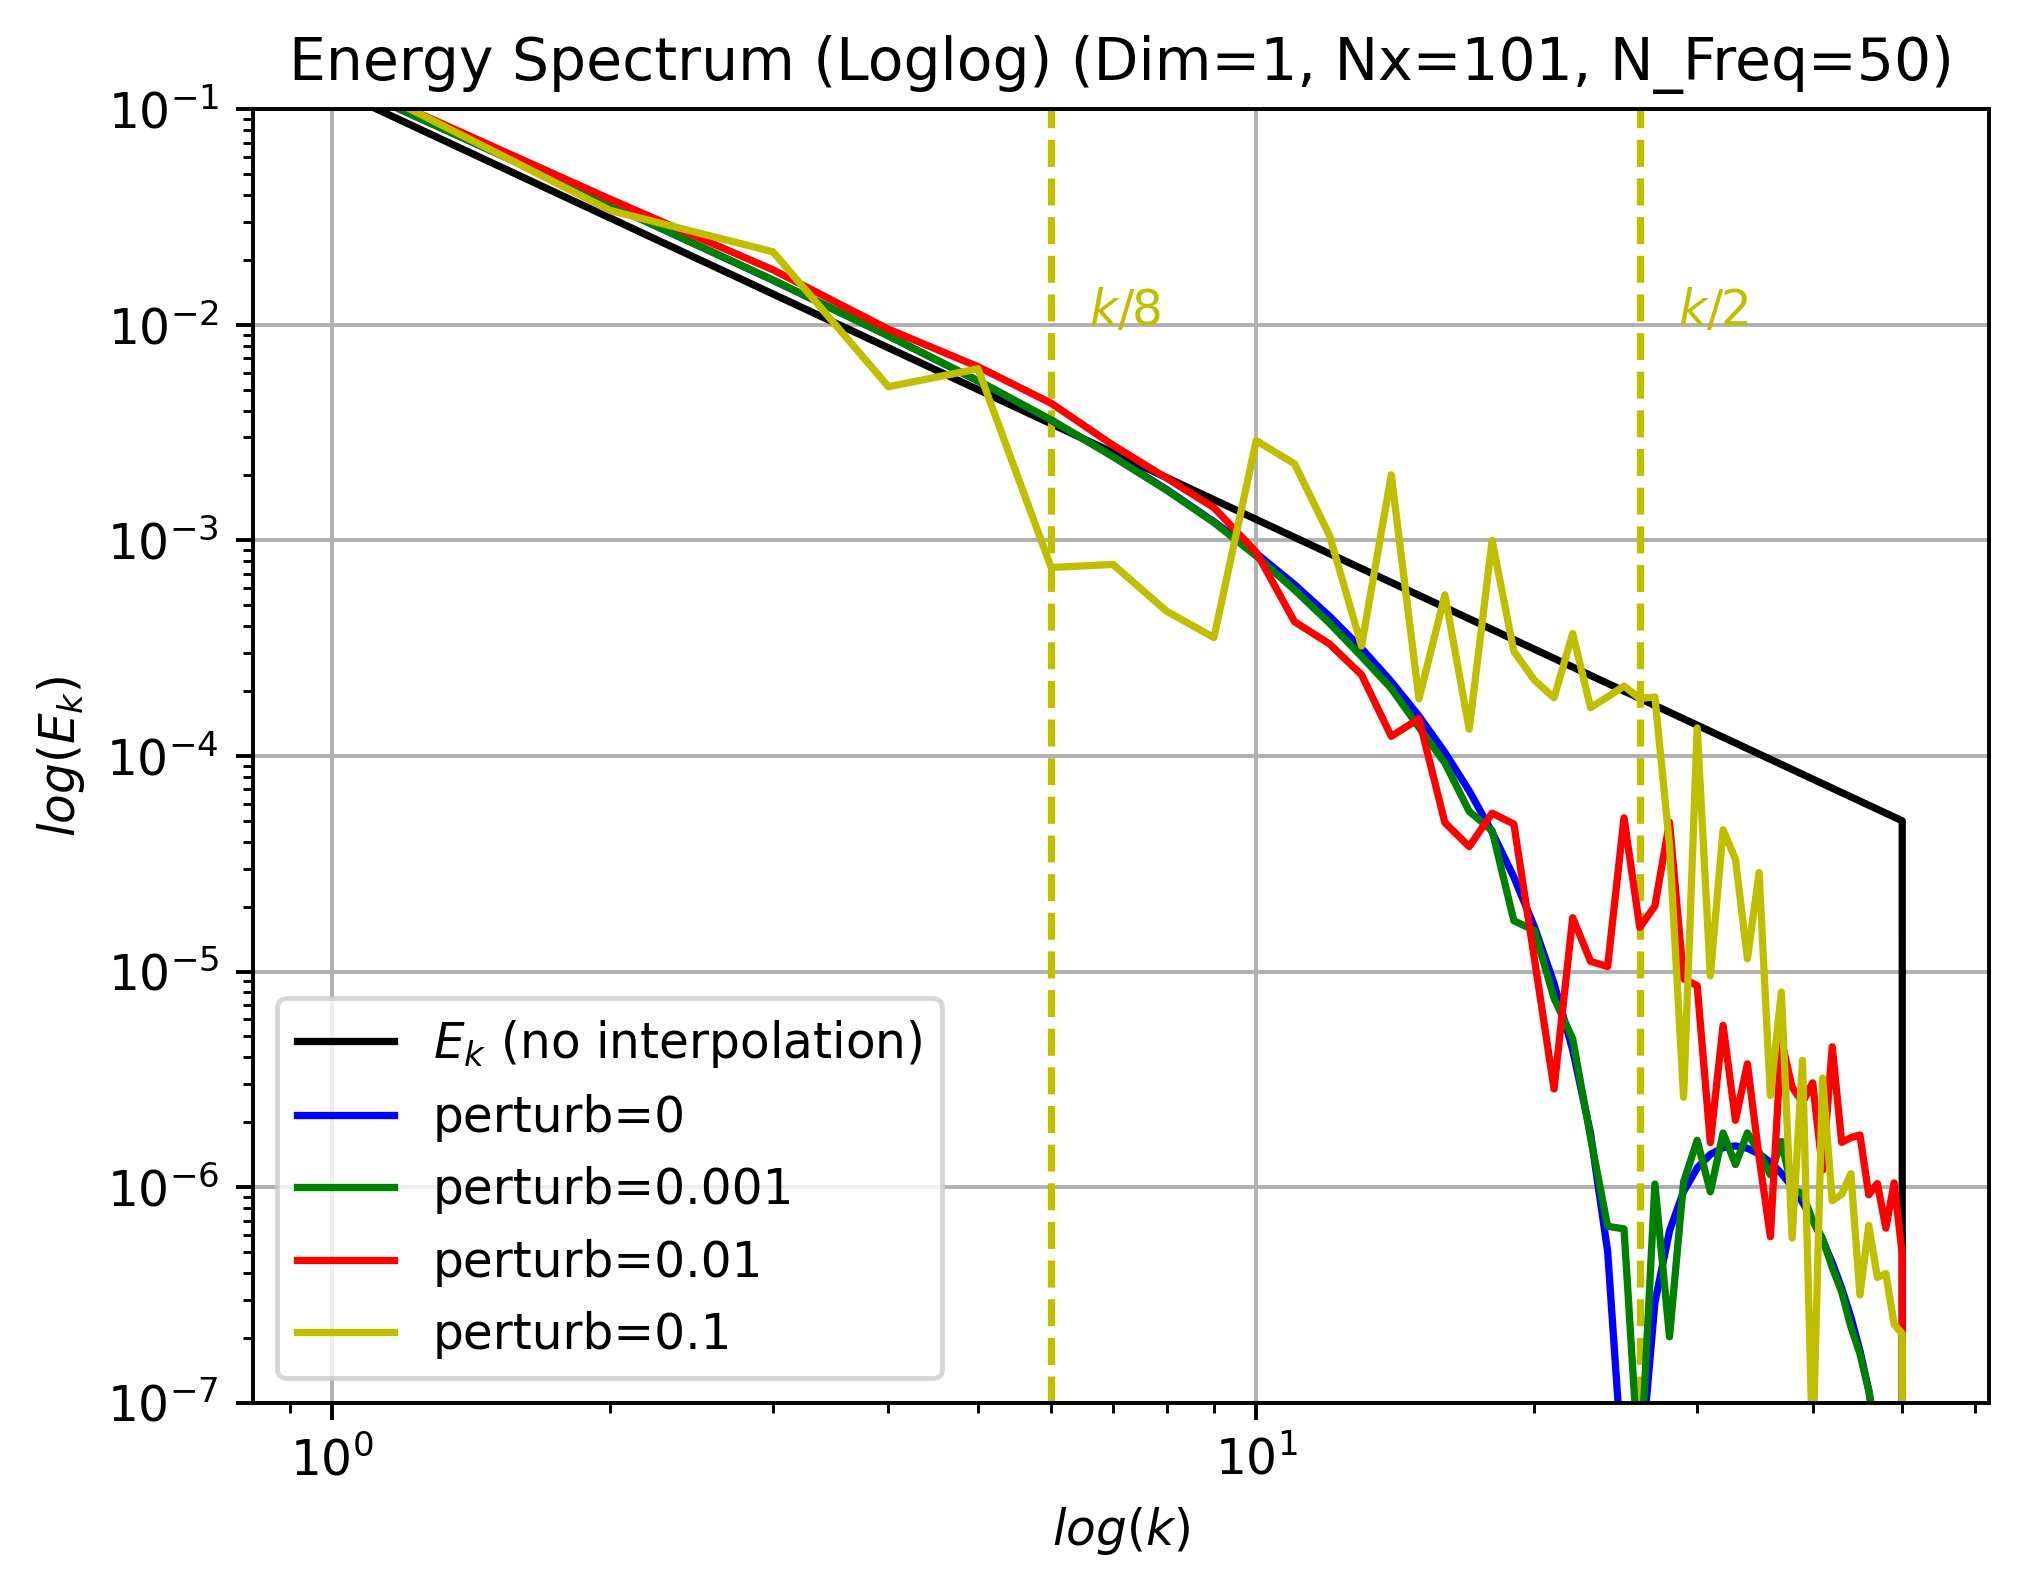
\includegraphics[width=6cm]{Code-Figures/sin-vel-prof-pertub/Energy Spectrum (Loglog) (Dim=1, Nx=101, N_Freq=50).png}
      \caption{$1D$ $E(k)$ field}
    \end{subfigure}
    \begin{subfigure}{7cm}
      \centering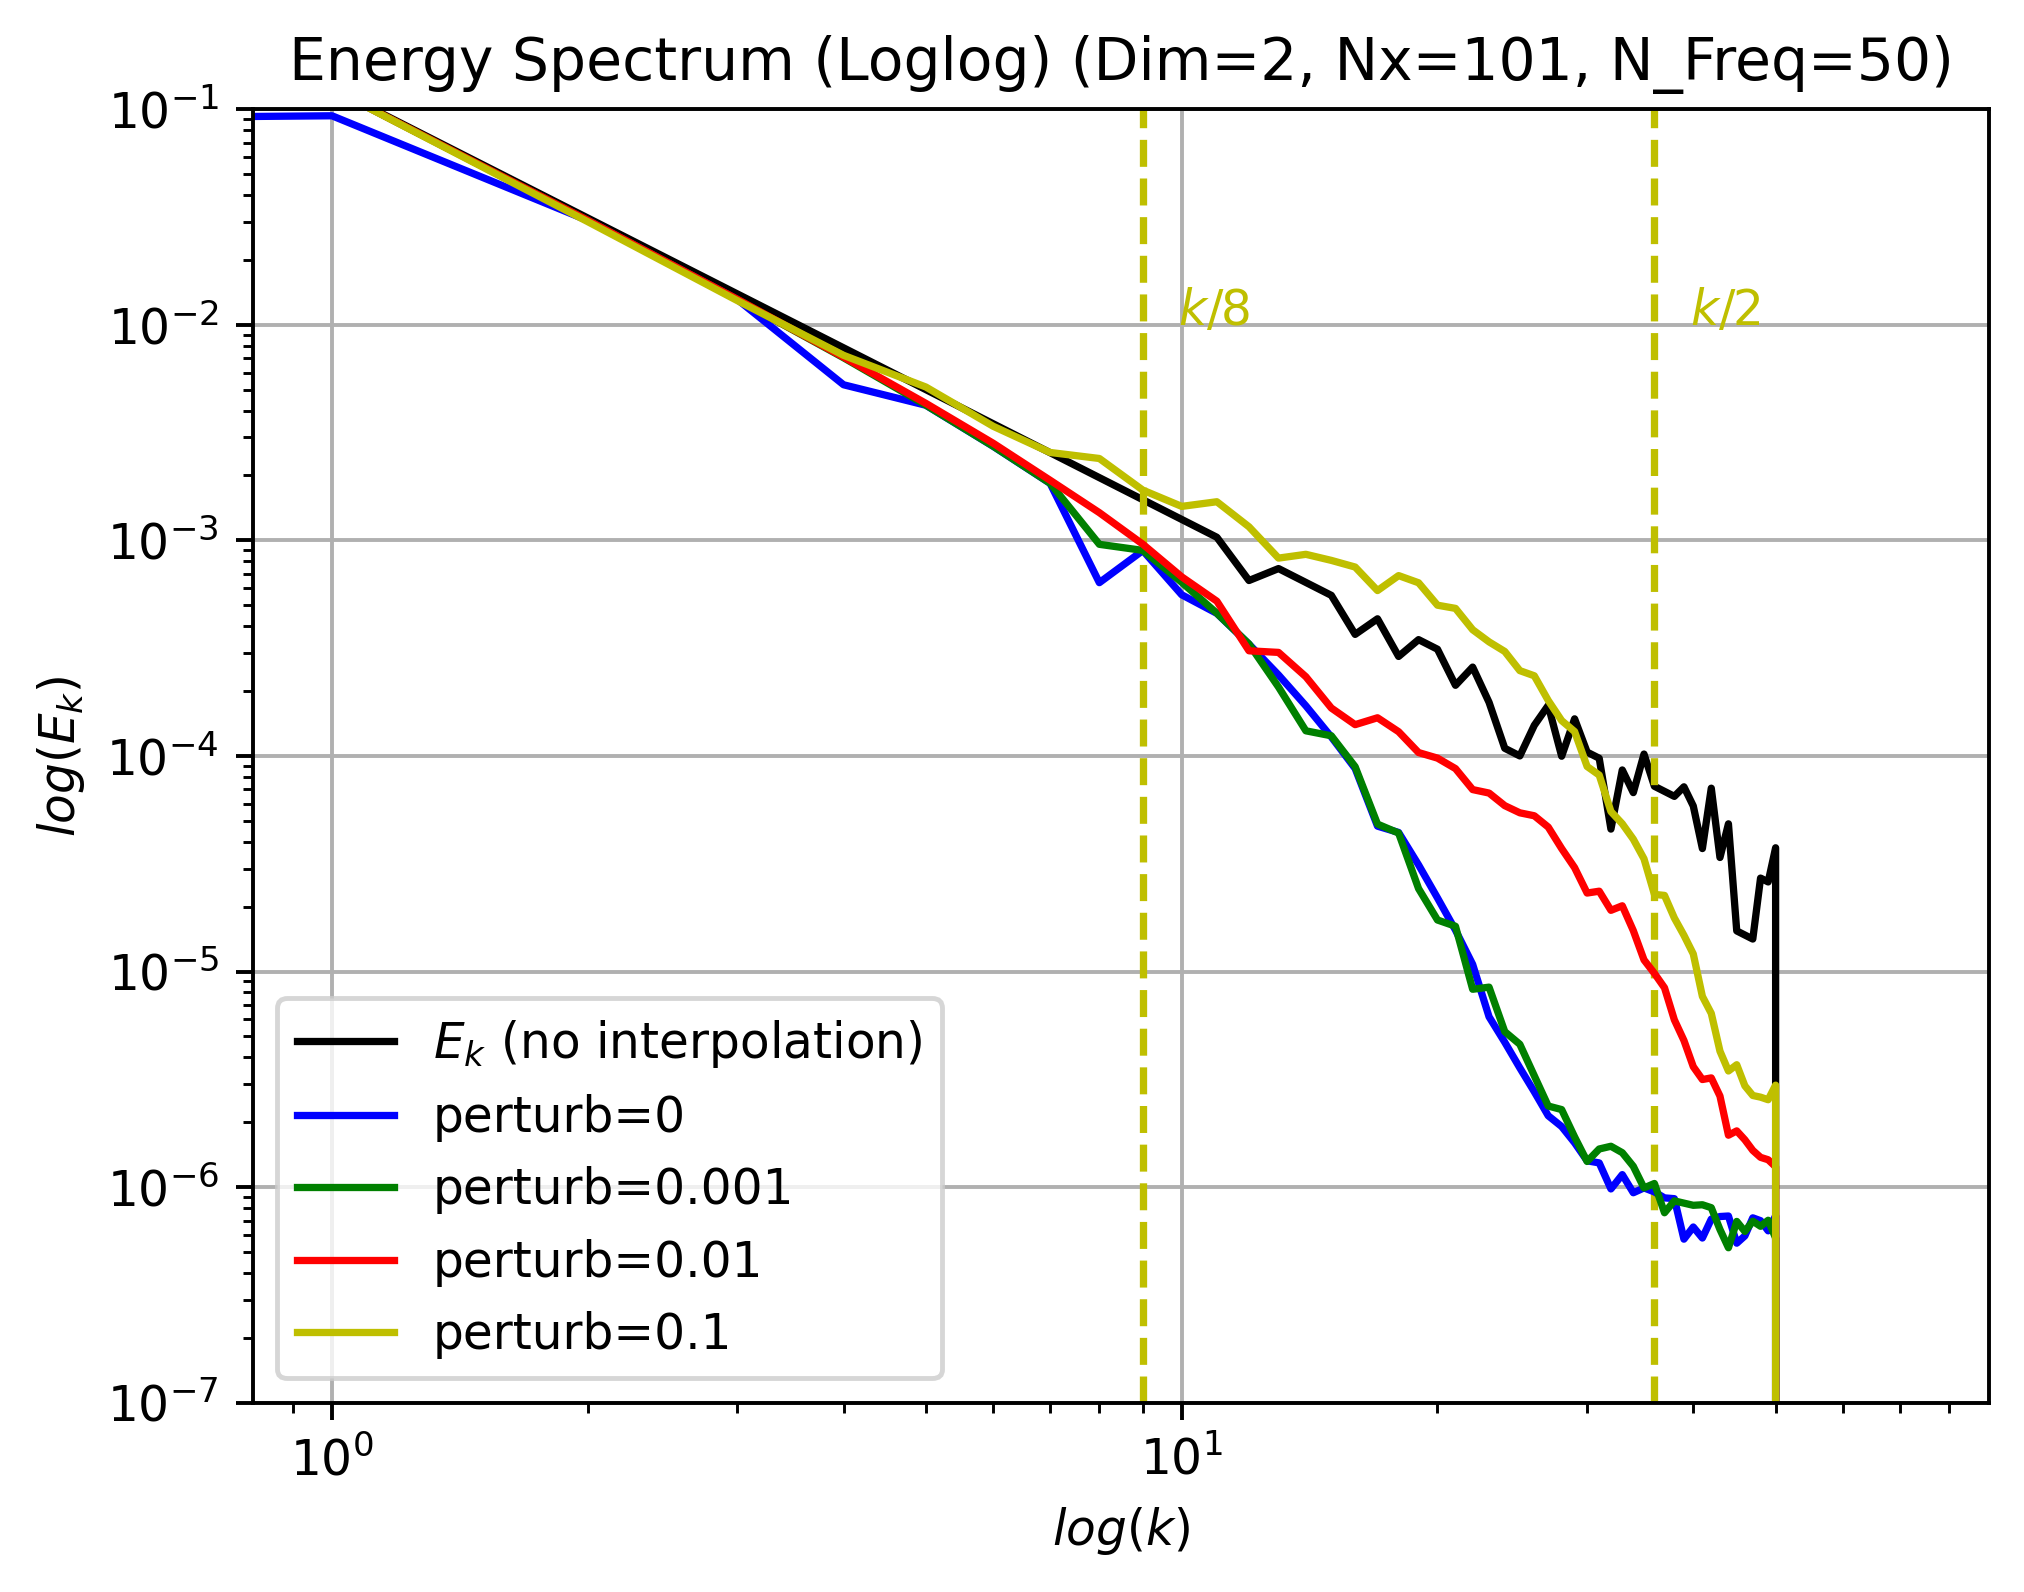
\includegraphics[width=6cm]{Code-Figures/sin-vel-prof-pertub/Energy Spectrum (Loglog) (Dim=2, Nx=101, N_Freq=50).png}
      \caption{$2D$ $E(k)$ field}
    \end{subfigure}
    \begin{subfigure}{7cm}
        \centering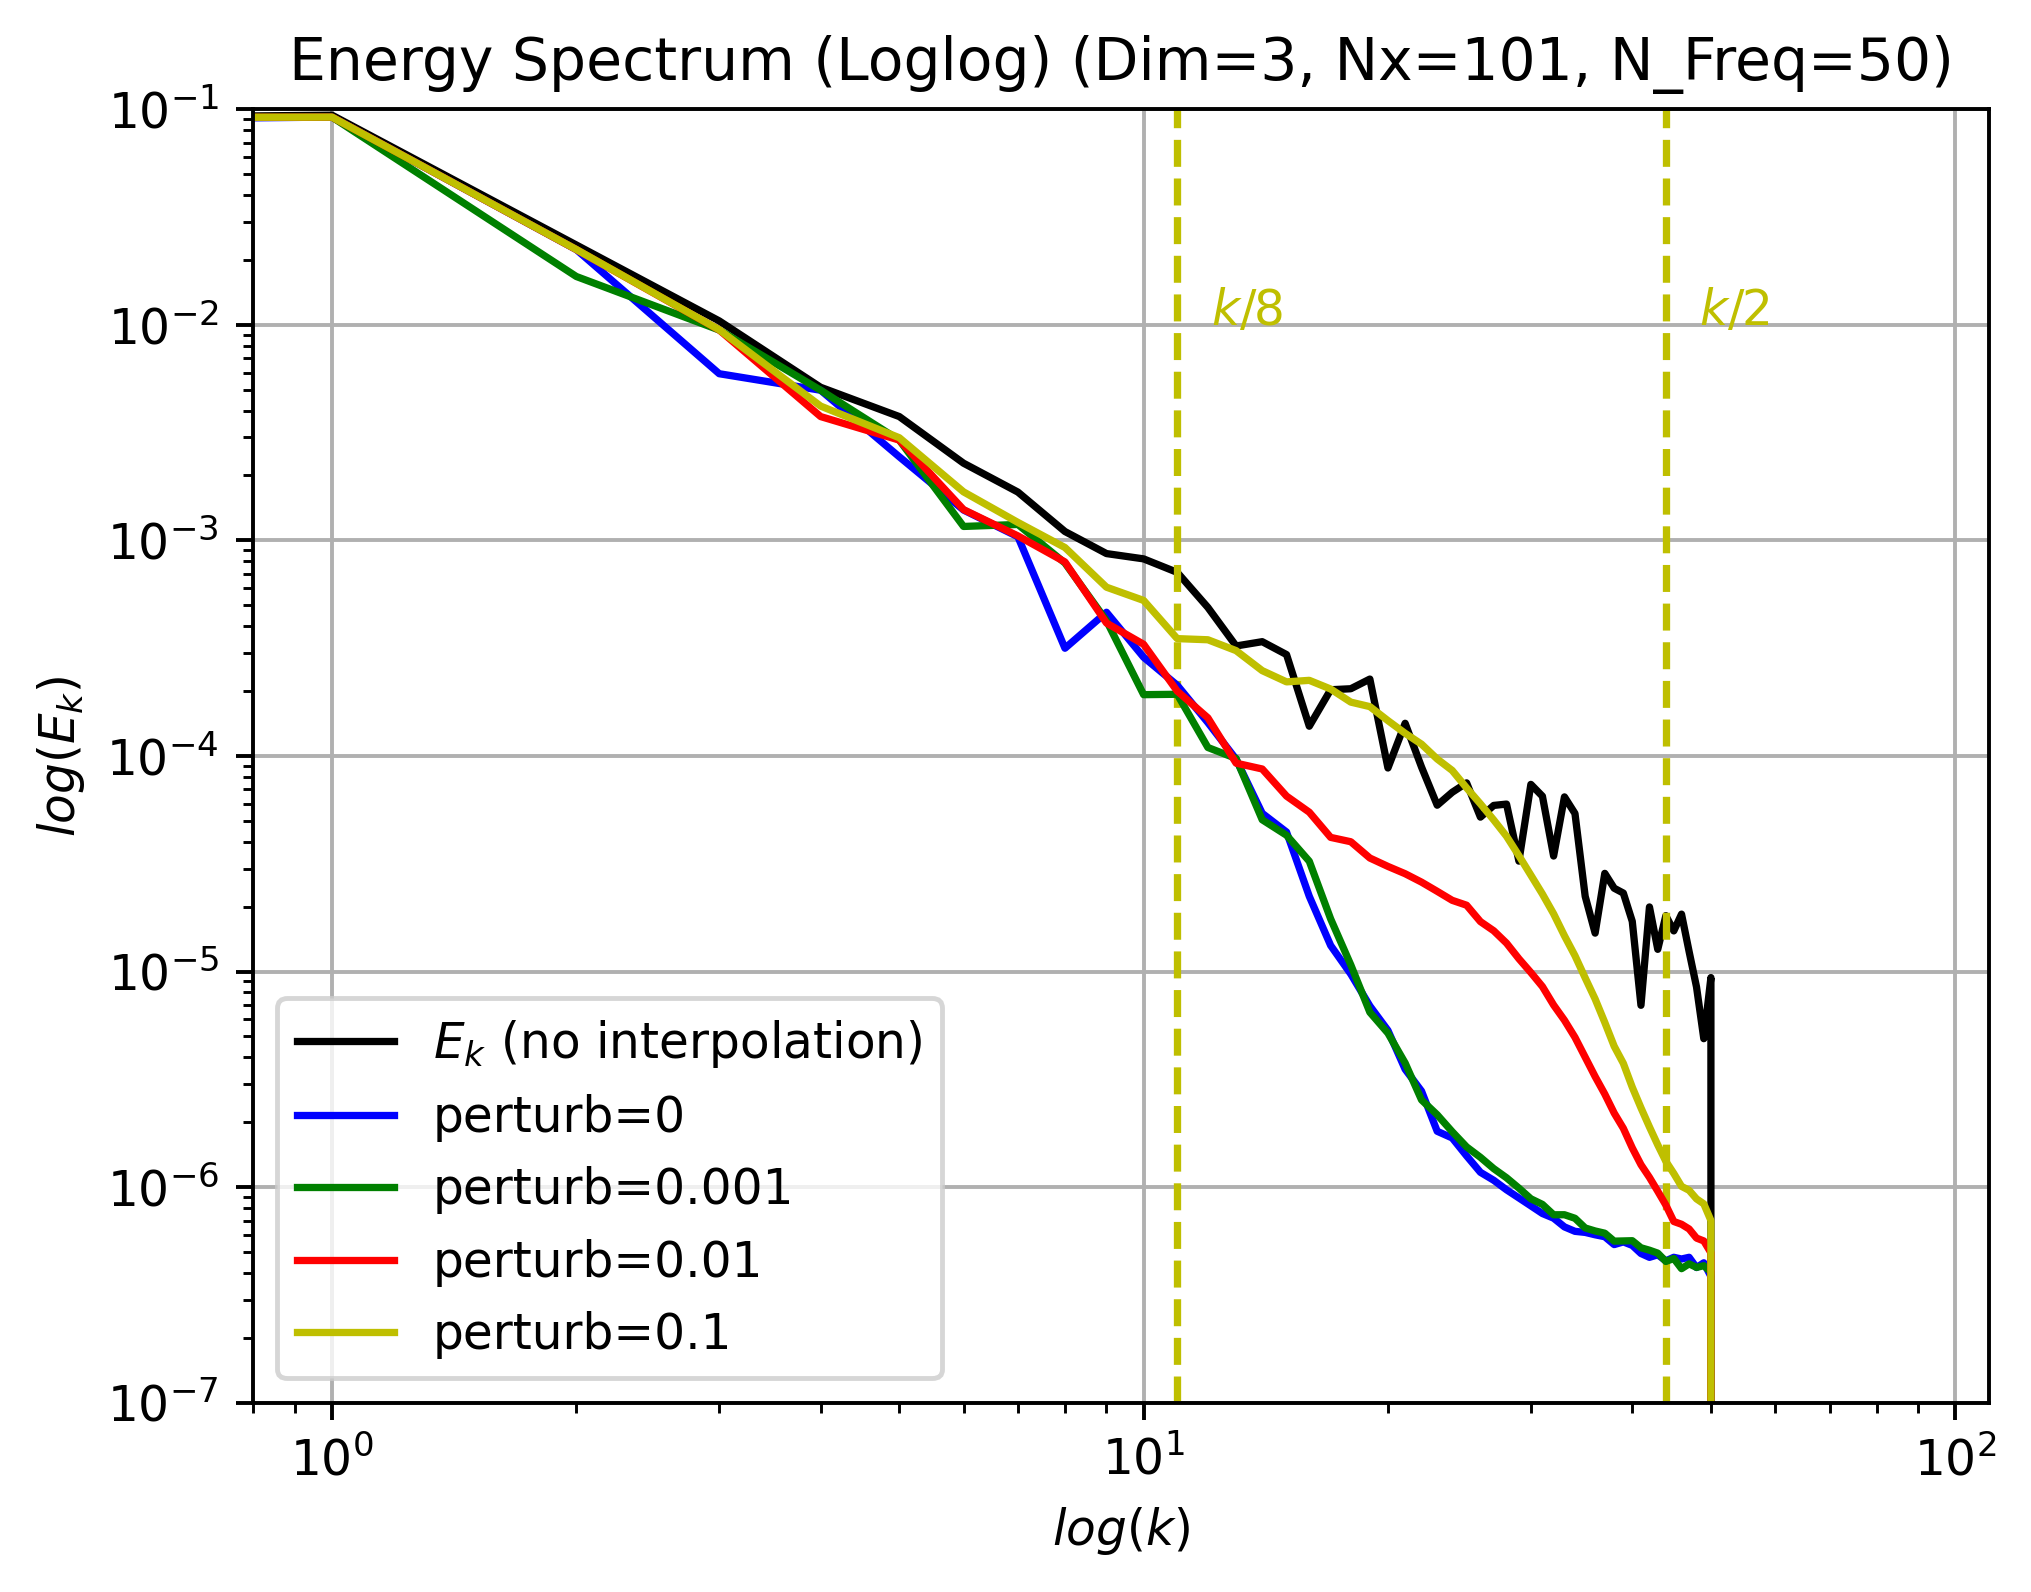
\includegraphics[width=6cm]{Code-Figures/sin-vel-prof-pertub/Energy Spectrum (Loglog) (Dim=3, Nx=101, N_Freq=50).png}
        \caption{$3D$ $E(k)$ field}
      \end{subfigure}
    \caption{The scalar fields $E(k)$ for $1D$, $2D$, and $3D$ case, for various perturbation amplitudes.}
    \label{fig:espec-scalar-fields-per-ampl}
\end{figure}

Then, in order to measure the effect of the interpolation scheme on the computed energy spectrum, the following interpolation schemes were considered:
\begin{itemize}
    \item \texttt{sph}:
    \begin{equation}
        \hat{\phi_i} = \sum_{ij} \frac{m_j}{\rho_j} \phi_j \DWIJ,
    \end{equation}
    
    \item \texttt{shepard}:
    \begin{equation}
        \hat{\phi_i} = \frac{\sum_{ij} \phi_j \WIJ}{\sum_{ij} \WIJ},
    \end{equation}

    \item \texttt{order1} \parencite{Liu2006}:
    \begin{equation}
      \tensor{A}_{4 \times 4} \vect{x}_{4 \times 1} = \vect{b}_{4 \times 1}
      \label{eq:interp-order1}
    \end{equation}
    where, $\tensor{A}$ is the moment matrix, $\vect{b} = [\phi, \nabla \phi]^T$ is the interpolated property and its gradient calculated using basic SPH, and $\vect{x} = [\hat{\phi}, \nabla \hat{\phi}]^T$ is the unknown interpolated property and its gradient,

    \item \texttt{order1BL}: same as \Eqref{eq:interp-order1}, but with the $\DWIJ$ term corrected using the Bonet-Lok correction \parencite{bonet1999variational},

    \item \texttt{order1MC}: same as \Eqref{eq:interp-order1}, but with the $\DWIJ$ term corrected using the Mixed-Kernel correction \parencite{bonet1999variational},
\end{itemize}
where $\phi$ is the quantity to be interpolated, and $\hat{\phi}$ is the interpolated quantity.

From the results shown in \figref{fig:espec-scalar-fields-i-methods}, it can be observed that the \texttt{order1MC} interpolation scheme, seems to introduce the least amount of energy at lower resolution scales, with the \texttt{sph} scheme introducing the most amount of energy at lower resolution scales. This trend seems to hold true, for all dimensions.
Therefore, considering the fact that the \texttt{sph} interpolation scheme would appear to counter the loss in energy at lower resolution scales, due to the act of interpolation, it is chosen as the default interpolation scheme for the computation of the energy spectrum.

\begin{figure}[htb!]
	\begin{subfigure}{7cm}
		\centering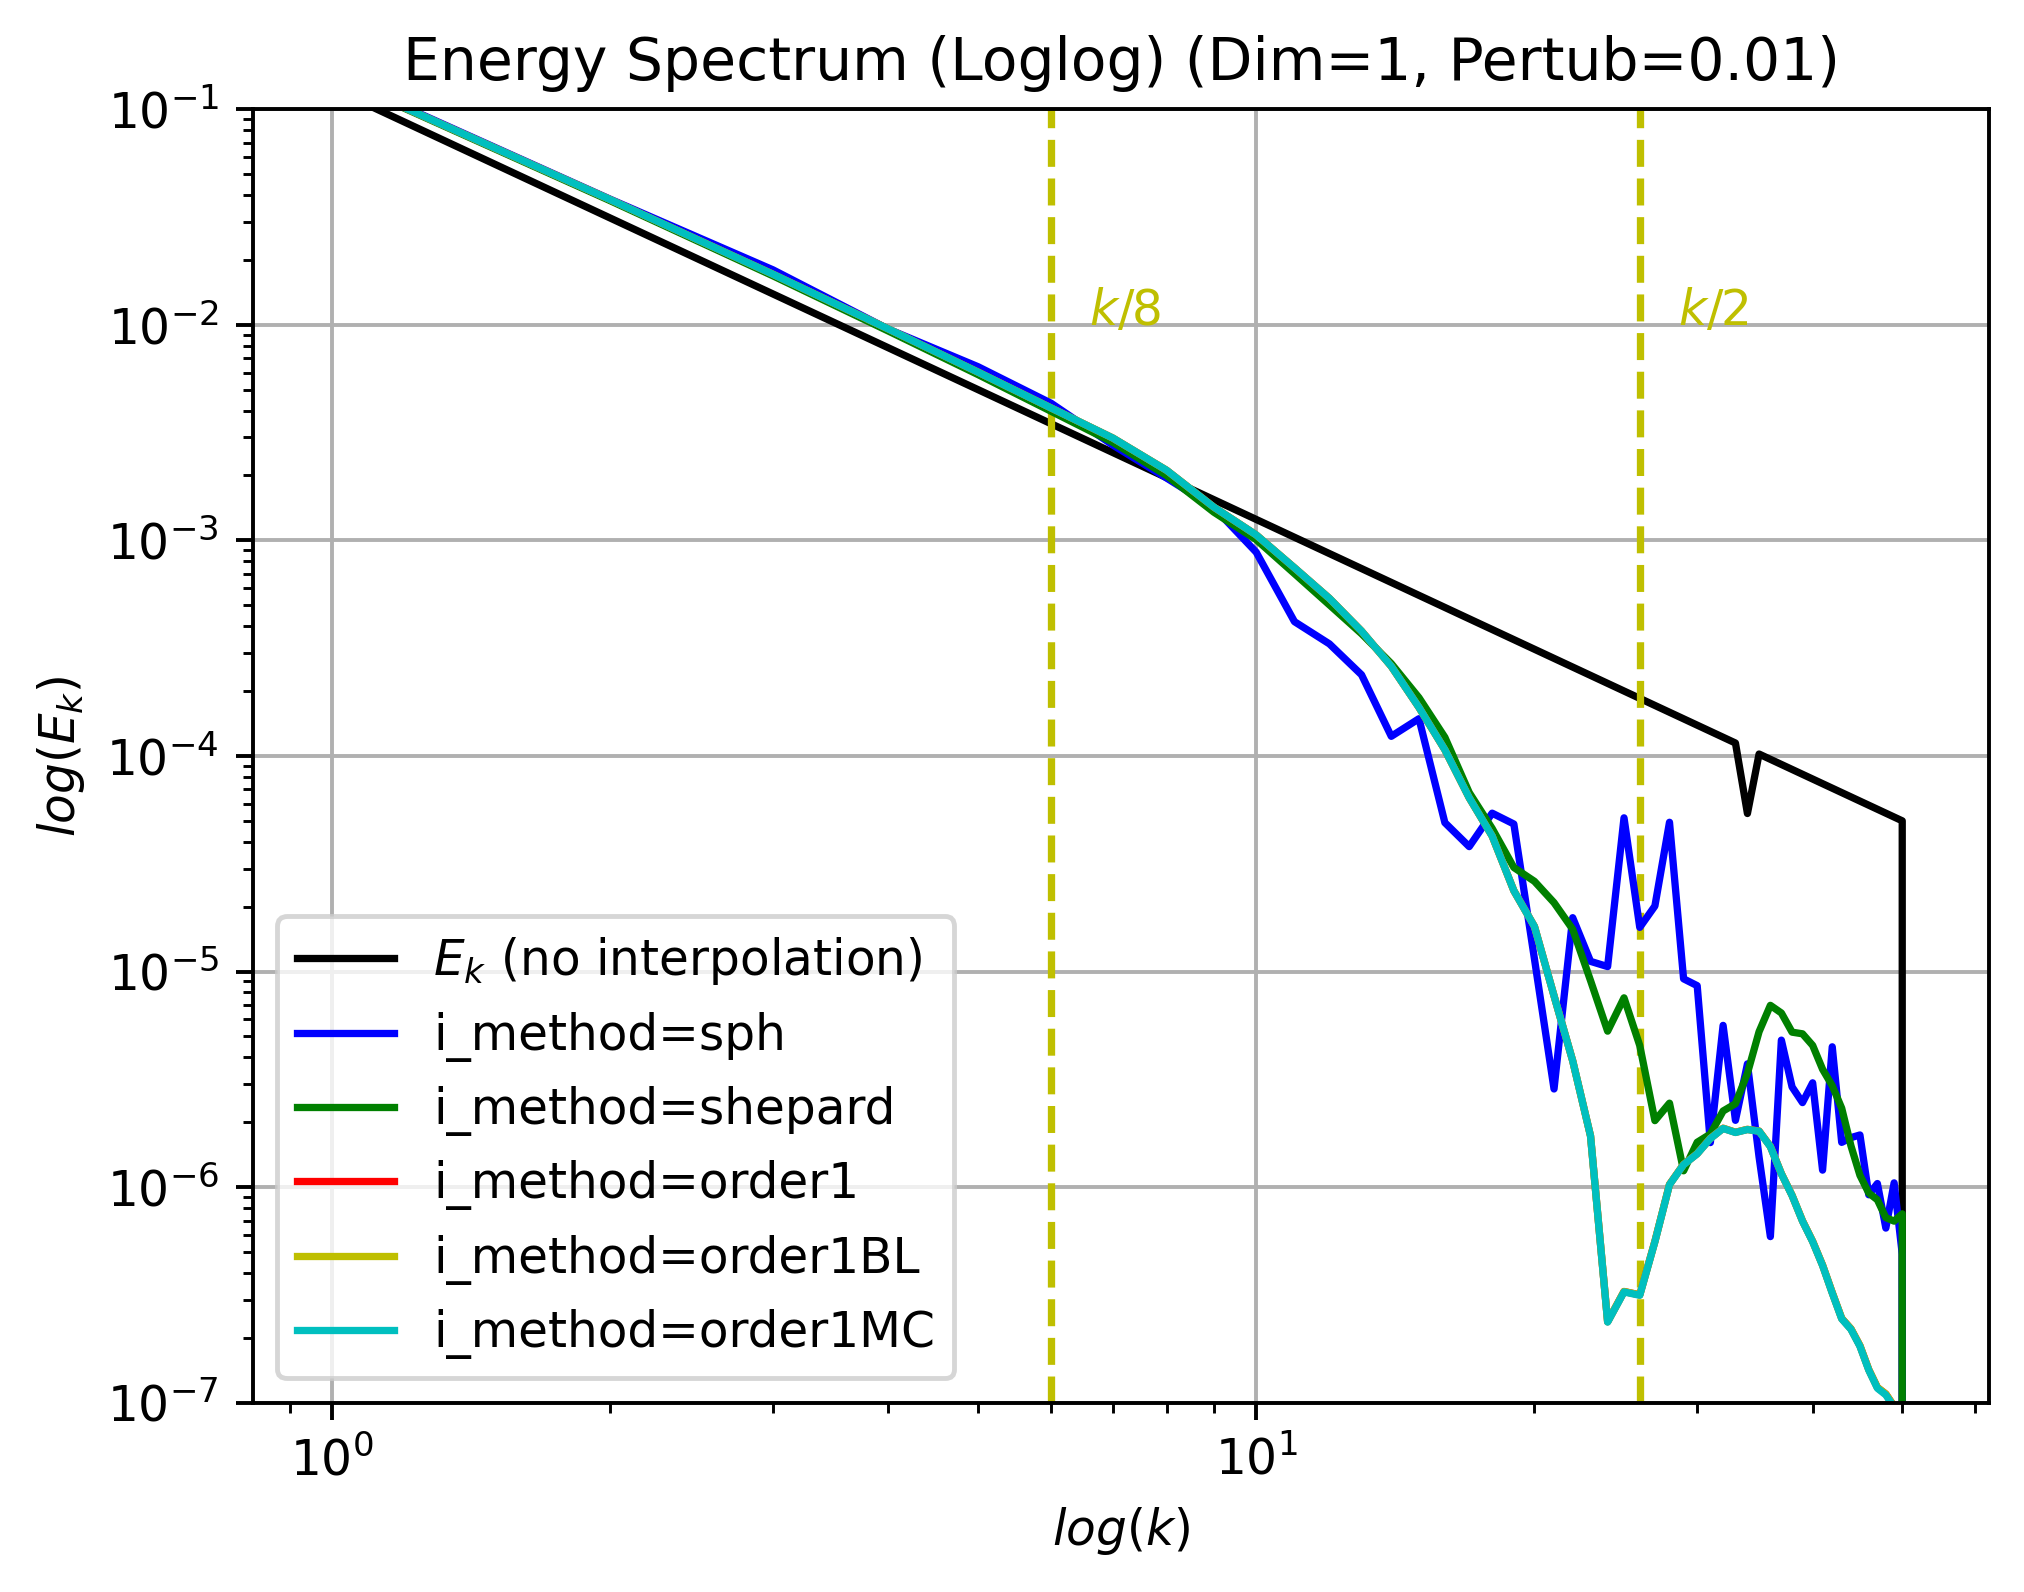
\includegraphics[width=6cm]{Code-Figures/sin-vel-prof-i-methods/Energy Spectrum (Loglog) (Dim=1, Pertub=0.01).png}
		\caption{$1D$ $E(k)$ field}
	\end{subfigure}
	\begin{subfigure}{7cm}
		\centering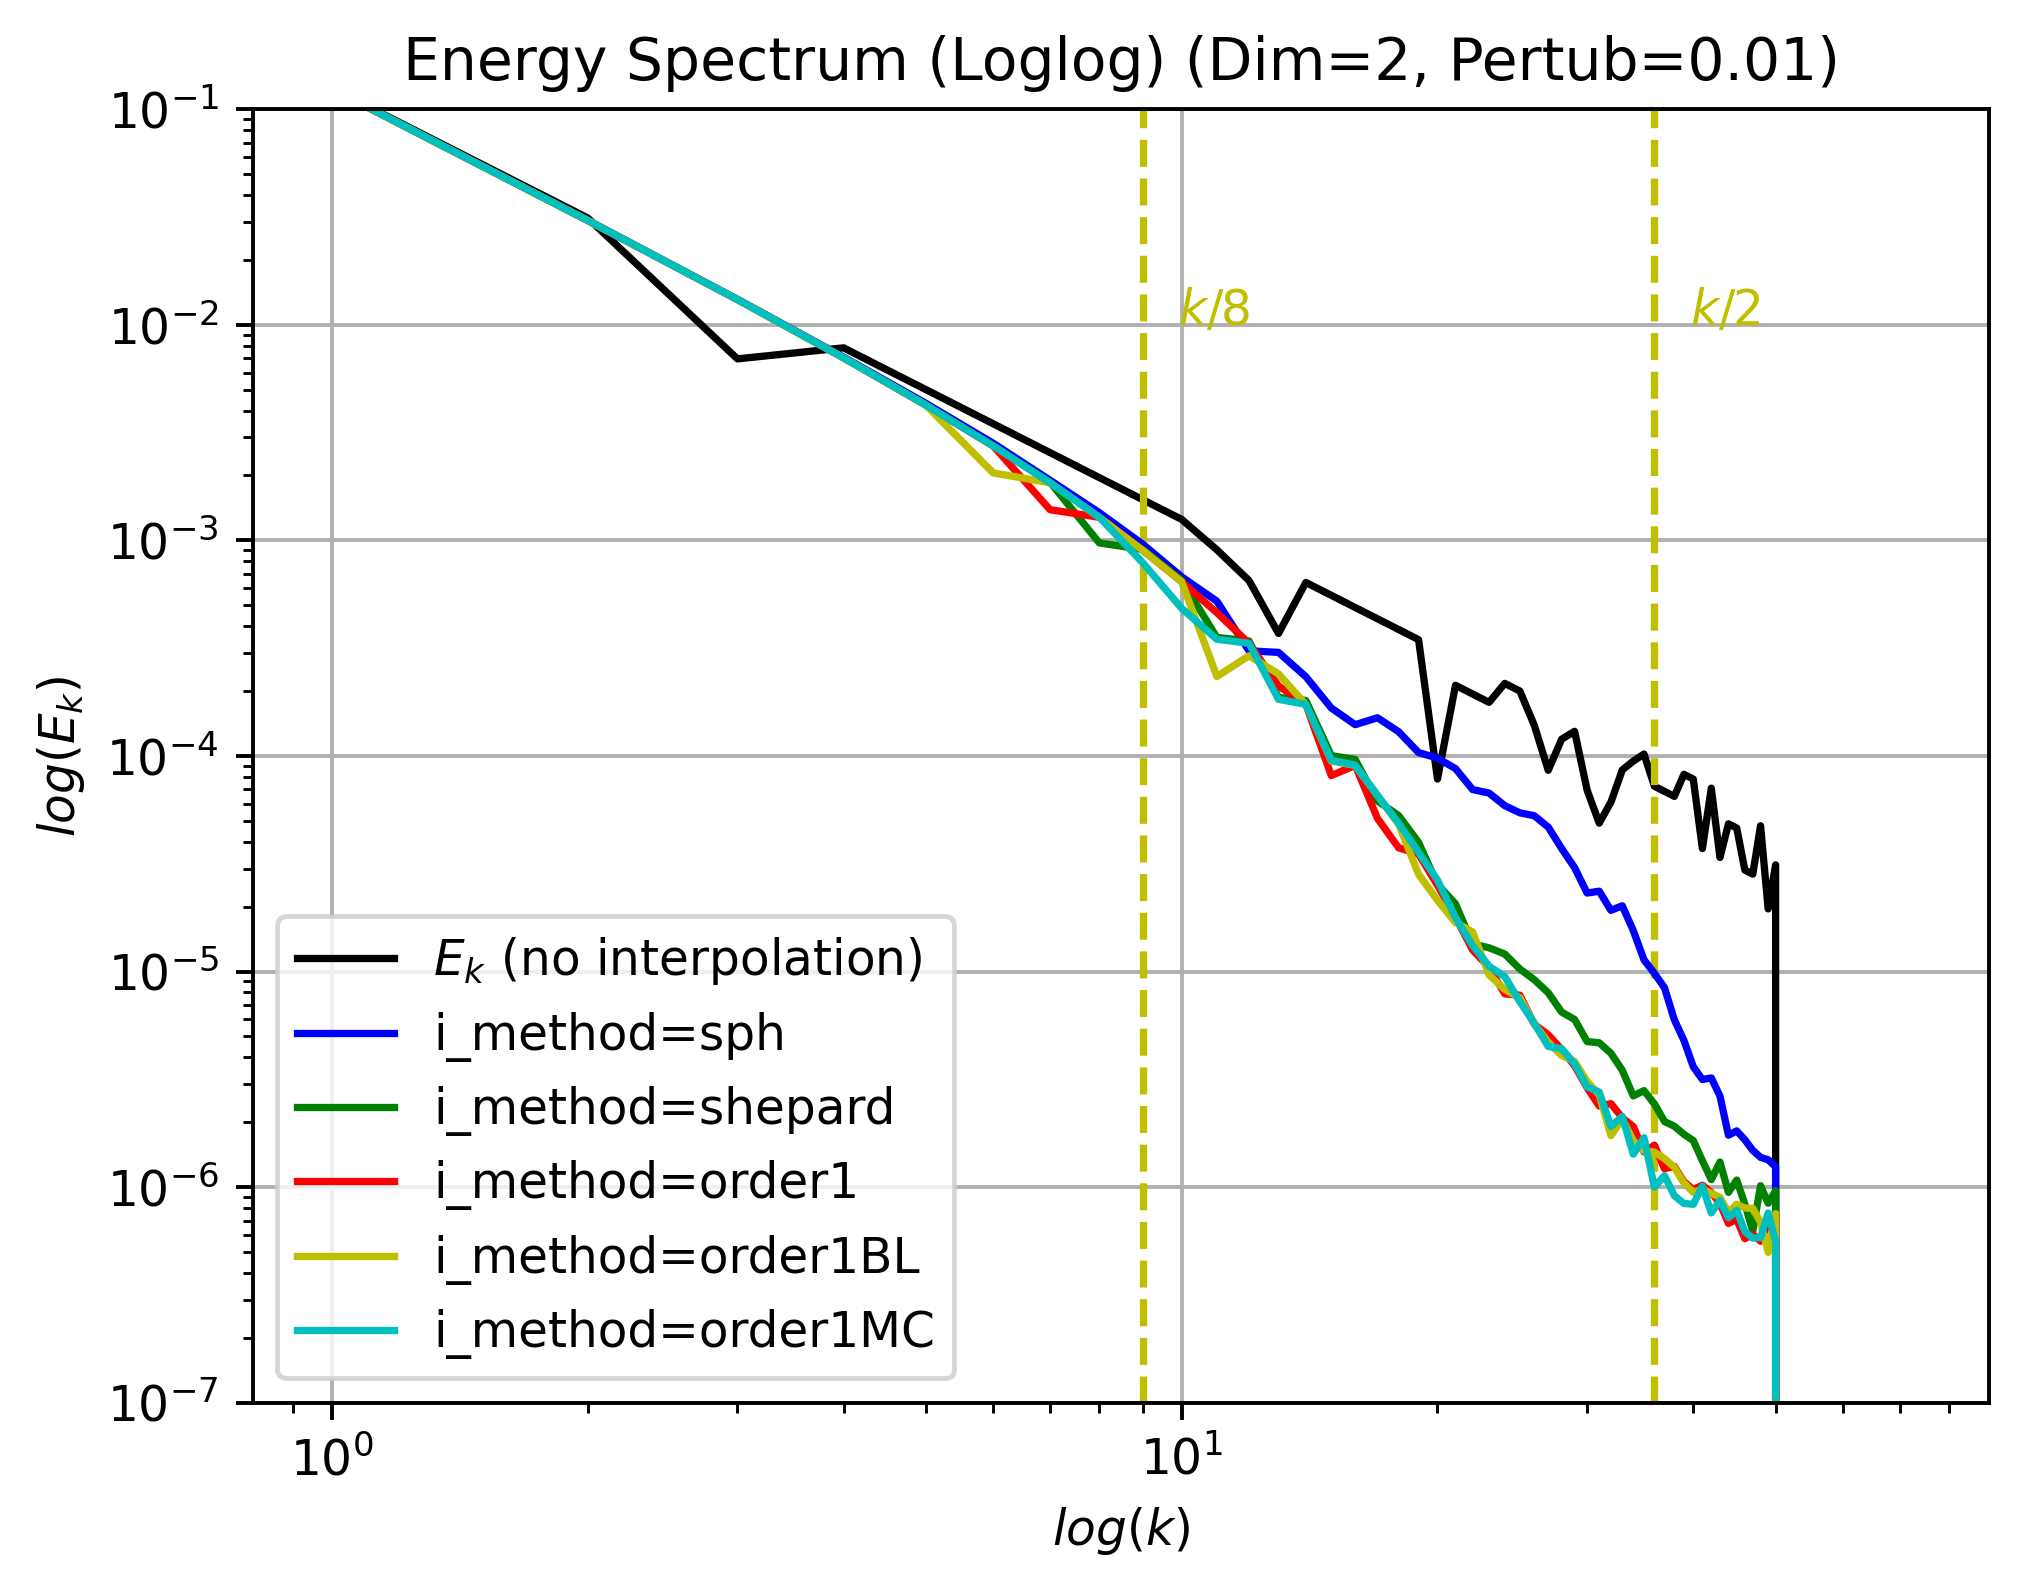
\includegraphics[width=6cm]{Code-Figures/sin-vel-prof-i-methods/Energy Spectrum (Loglog) (Dim=2, Pertub=0.01).png}
		\caption{$2D$ $E(k)$ field}
	\end{subfigure}
	\begin{subfigure}{7cm}
		\centering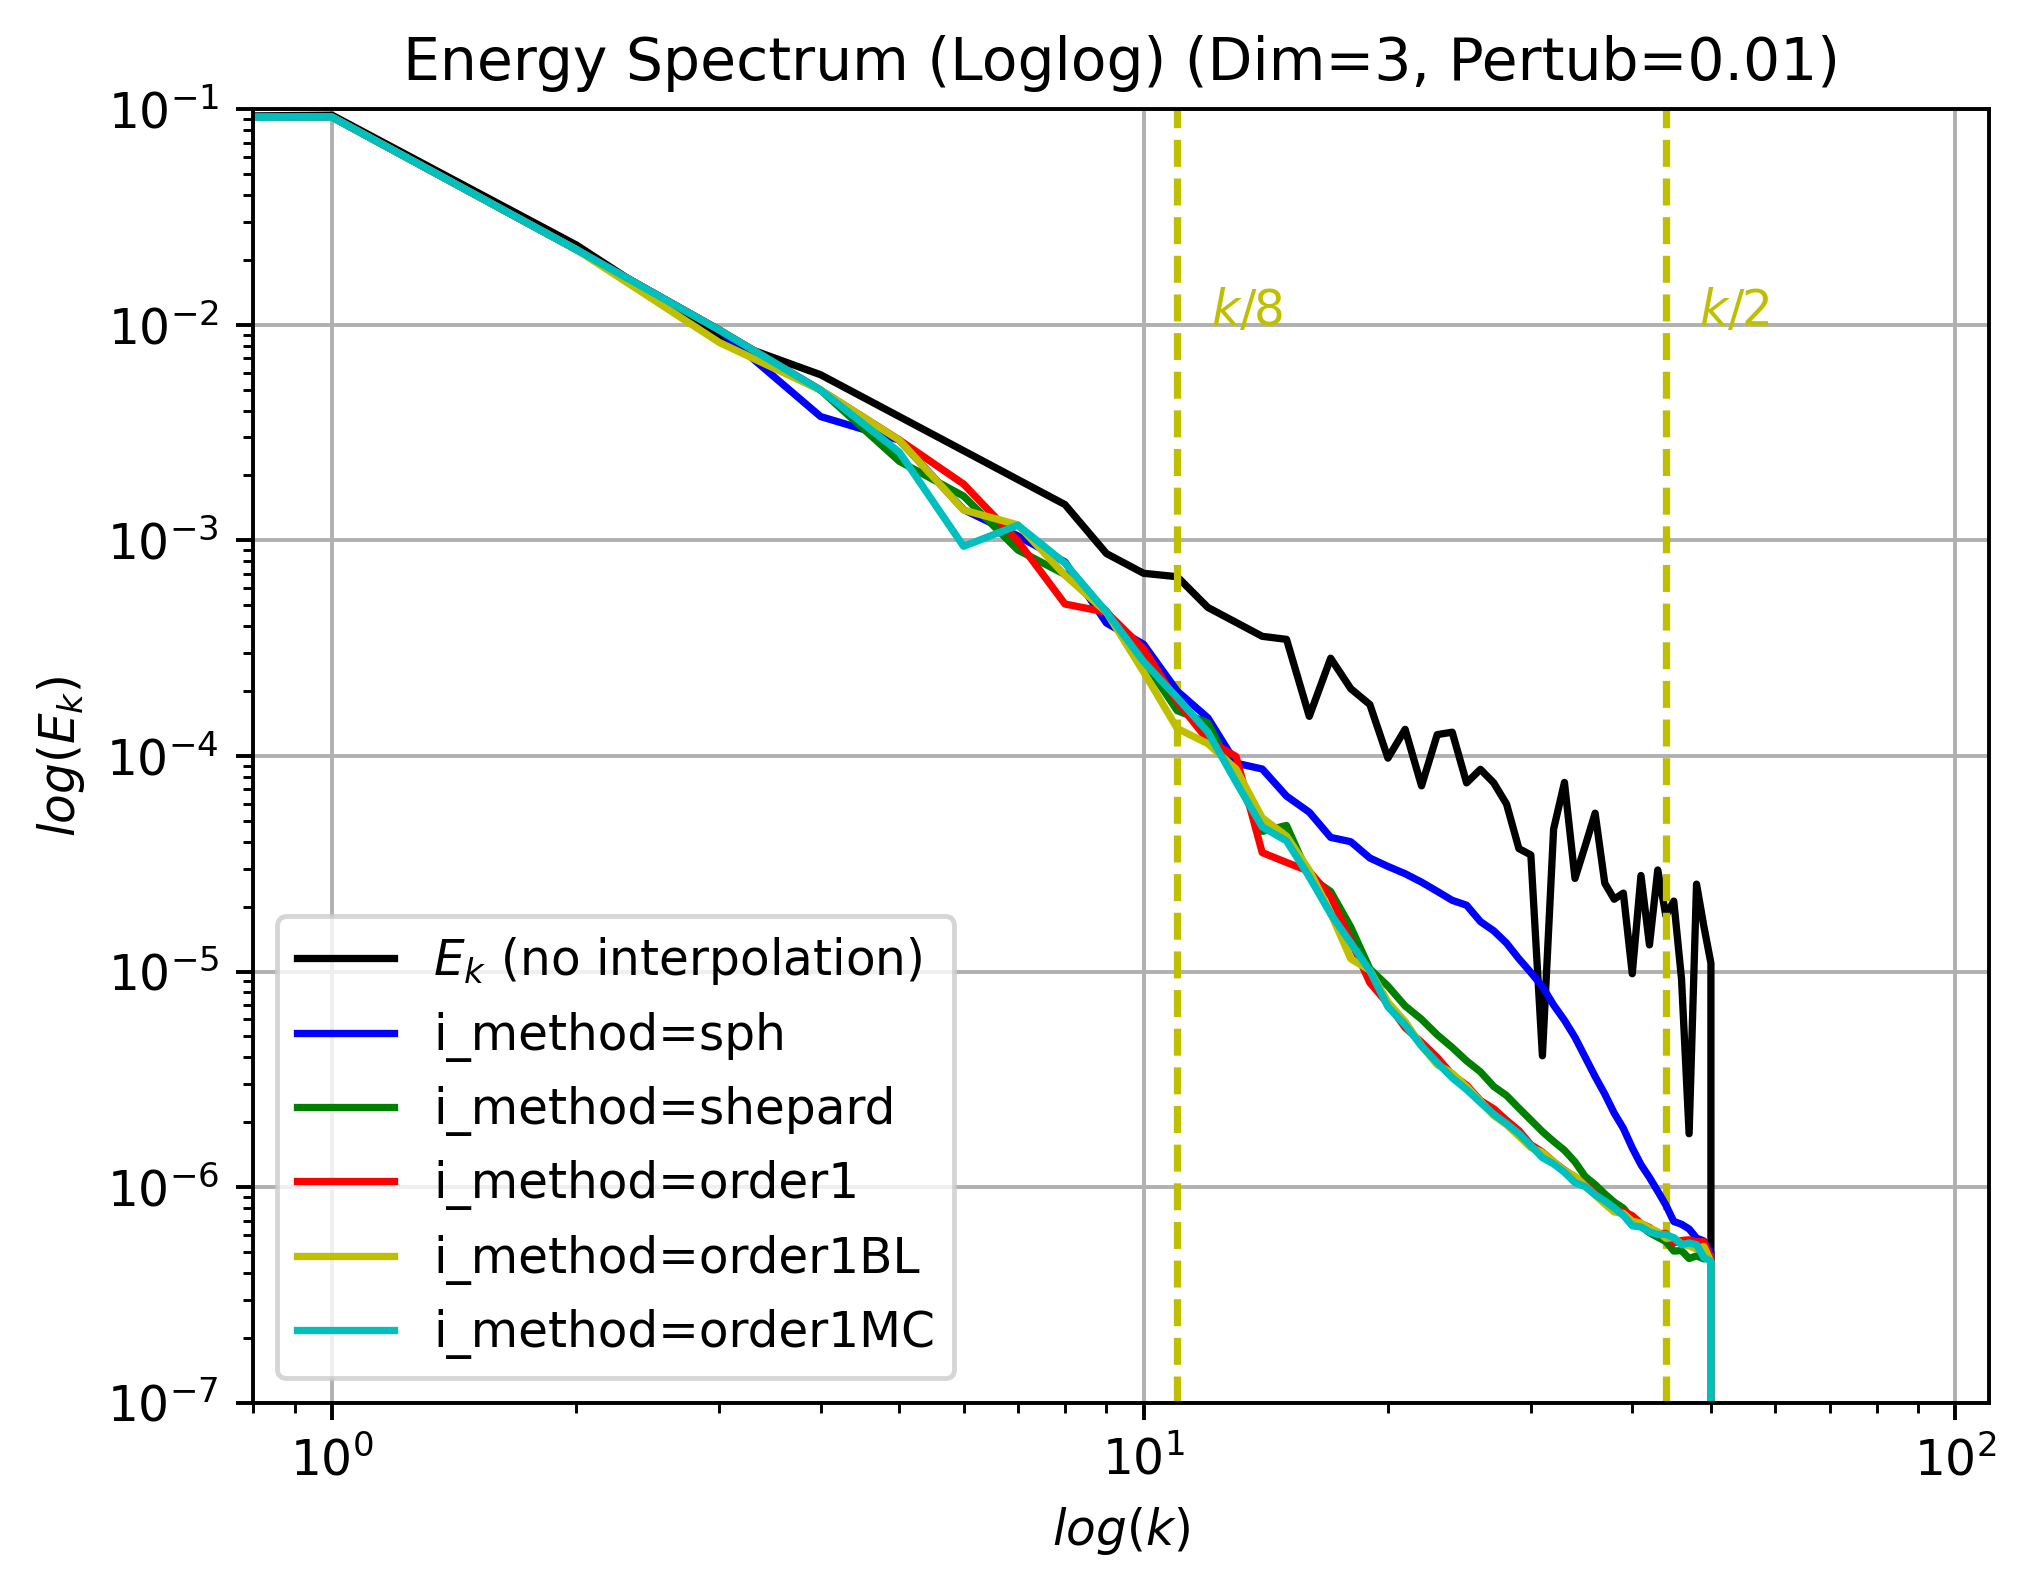
\includegraphics[width=6cm]{Code-Figures/sin-vel-prof-i-methods/Energy Spectrum (Loglog) (Dim=3, Pertub=0.01).png}
		\caption{$3D$ $E(k)$ field}
	\end{subfigure}
	\caption{The scalar fields $E(k)$ for $1D$, $2D$, and $3D$ case, for various interpolation schemes.}
	\label{fig:espec-scalar-fields-i-methods}
\end{figure}

Then, in order to measure the effect of the kernel on the computed energy spectrum, the following kernels were considered:
\begin{itemize}
    \item \texttt{CubicSpline},
    \item \texttt{WendlandQuinticC2},
    \item \texttt{WendlandQuinticC4},
    \item \texttt{WendlandQuinticC6},
    \item \texttt{Gaussian},
    \item \texttt{SuperGaussian},
    \item \texttt{QuinticSpline}.
\end{itemize}

From the results shown in \figref{fig:espec-scalar-fields-i-kernels}, it can be observed that the \texttt{Gaussian} kernel, seems to introduce the least amount of energy at lower resolution scales, with the \texttt{WendlandQuinticC6} kernel introducing the most amount of energy at lower resolution scales. This trend seems to hold true, for all dimensions.
Therefore, the \texttt{Gaussian} kernel is chosen as the default kernel for the computation of the energy spectrum.

\begin{figure}[htb!]
	\begin{subfigure}{7cm}
		\centering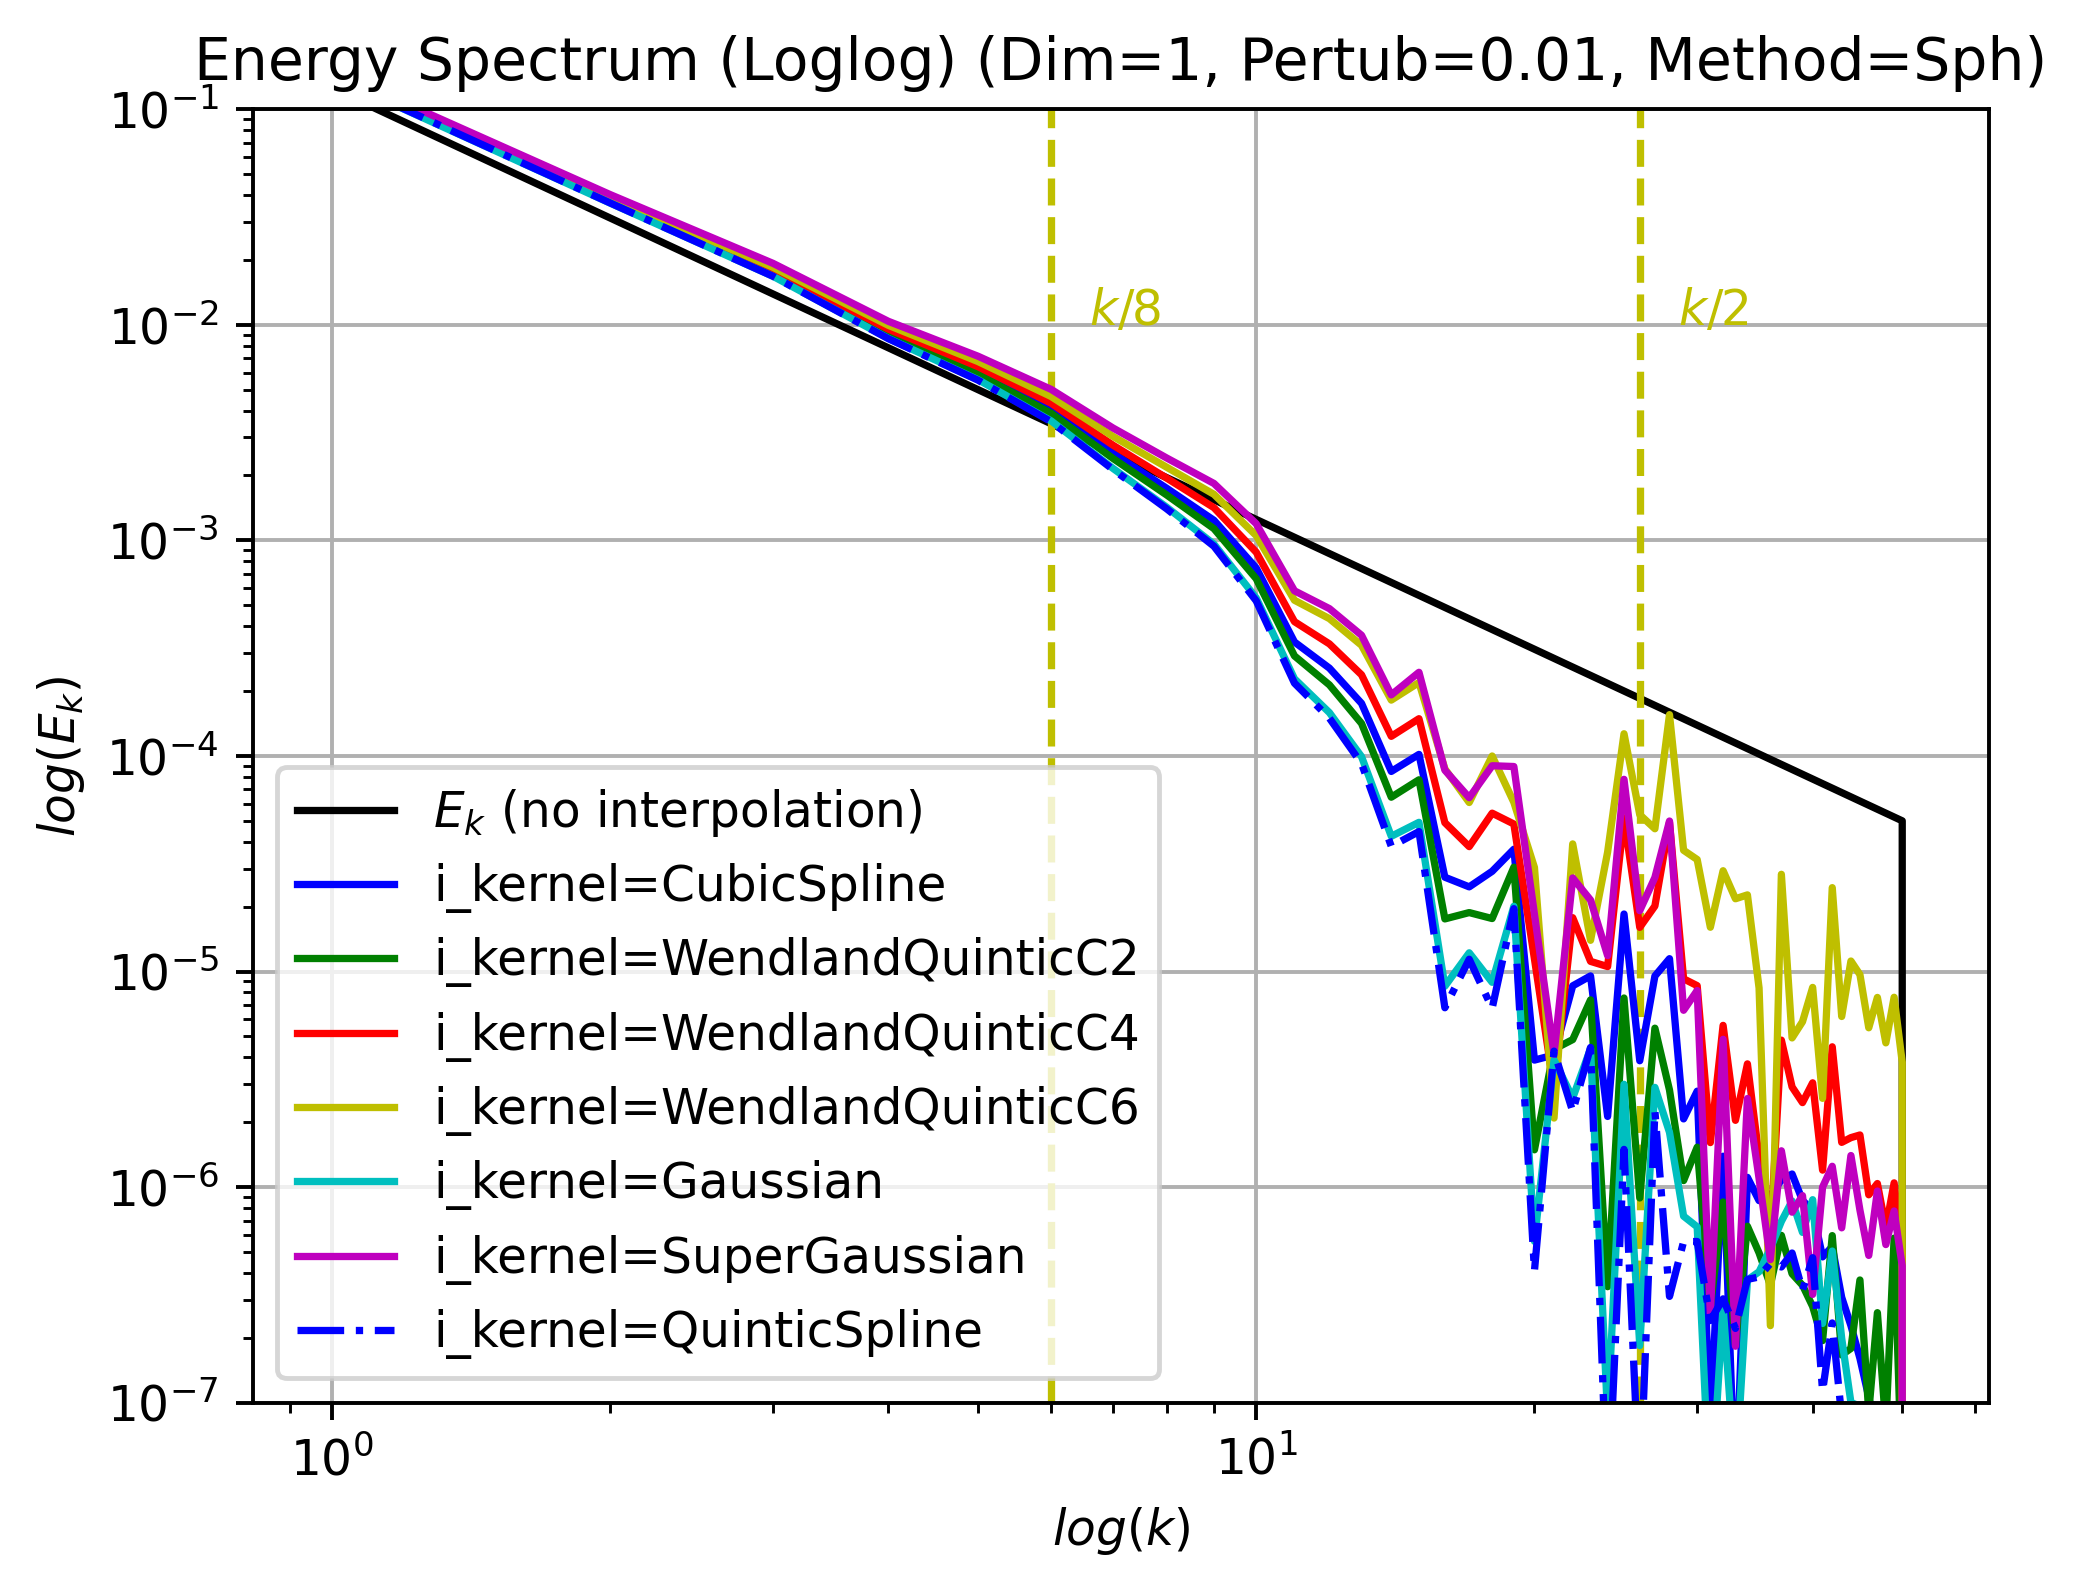
\includegraphics[width=6cm]{Code-Figures/sin-vel-prof-i-kernel/Energy Spectrum (Loglog) (Dim=1, Pertub=0.01, Method=Sph).png}
		\caption{$1D$ $E(k)$ field}
	\end{subfigure}
	\begin{subfigure}{7cm}
		\centering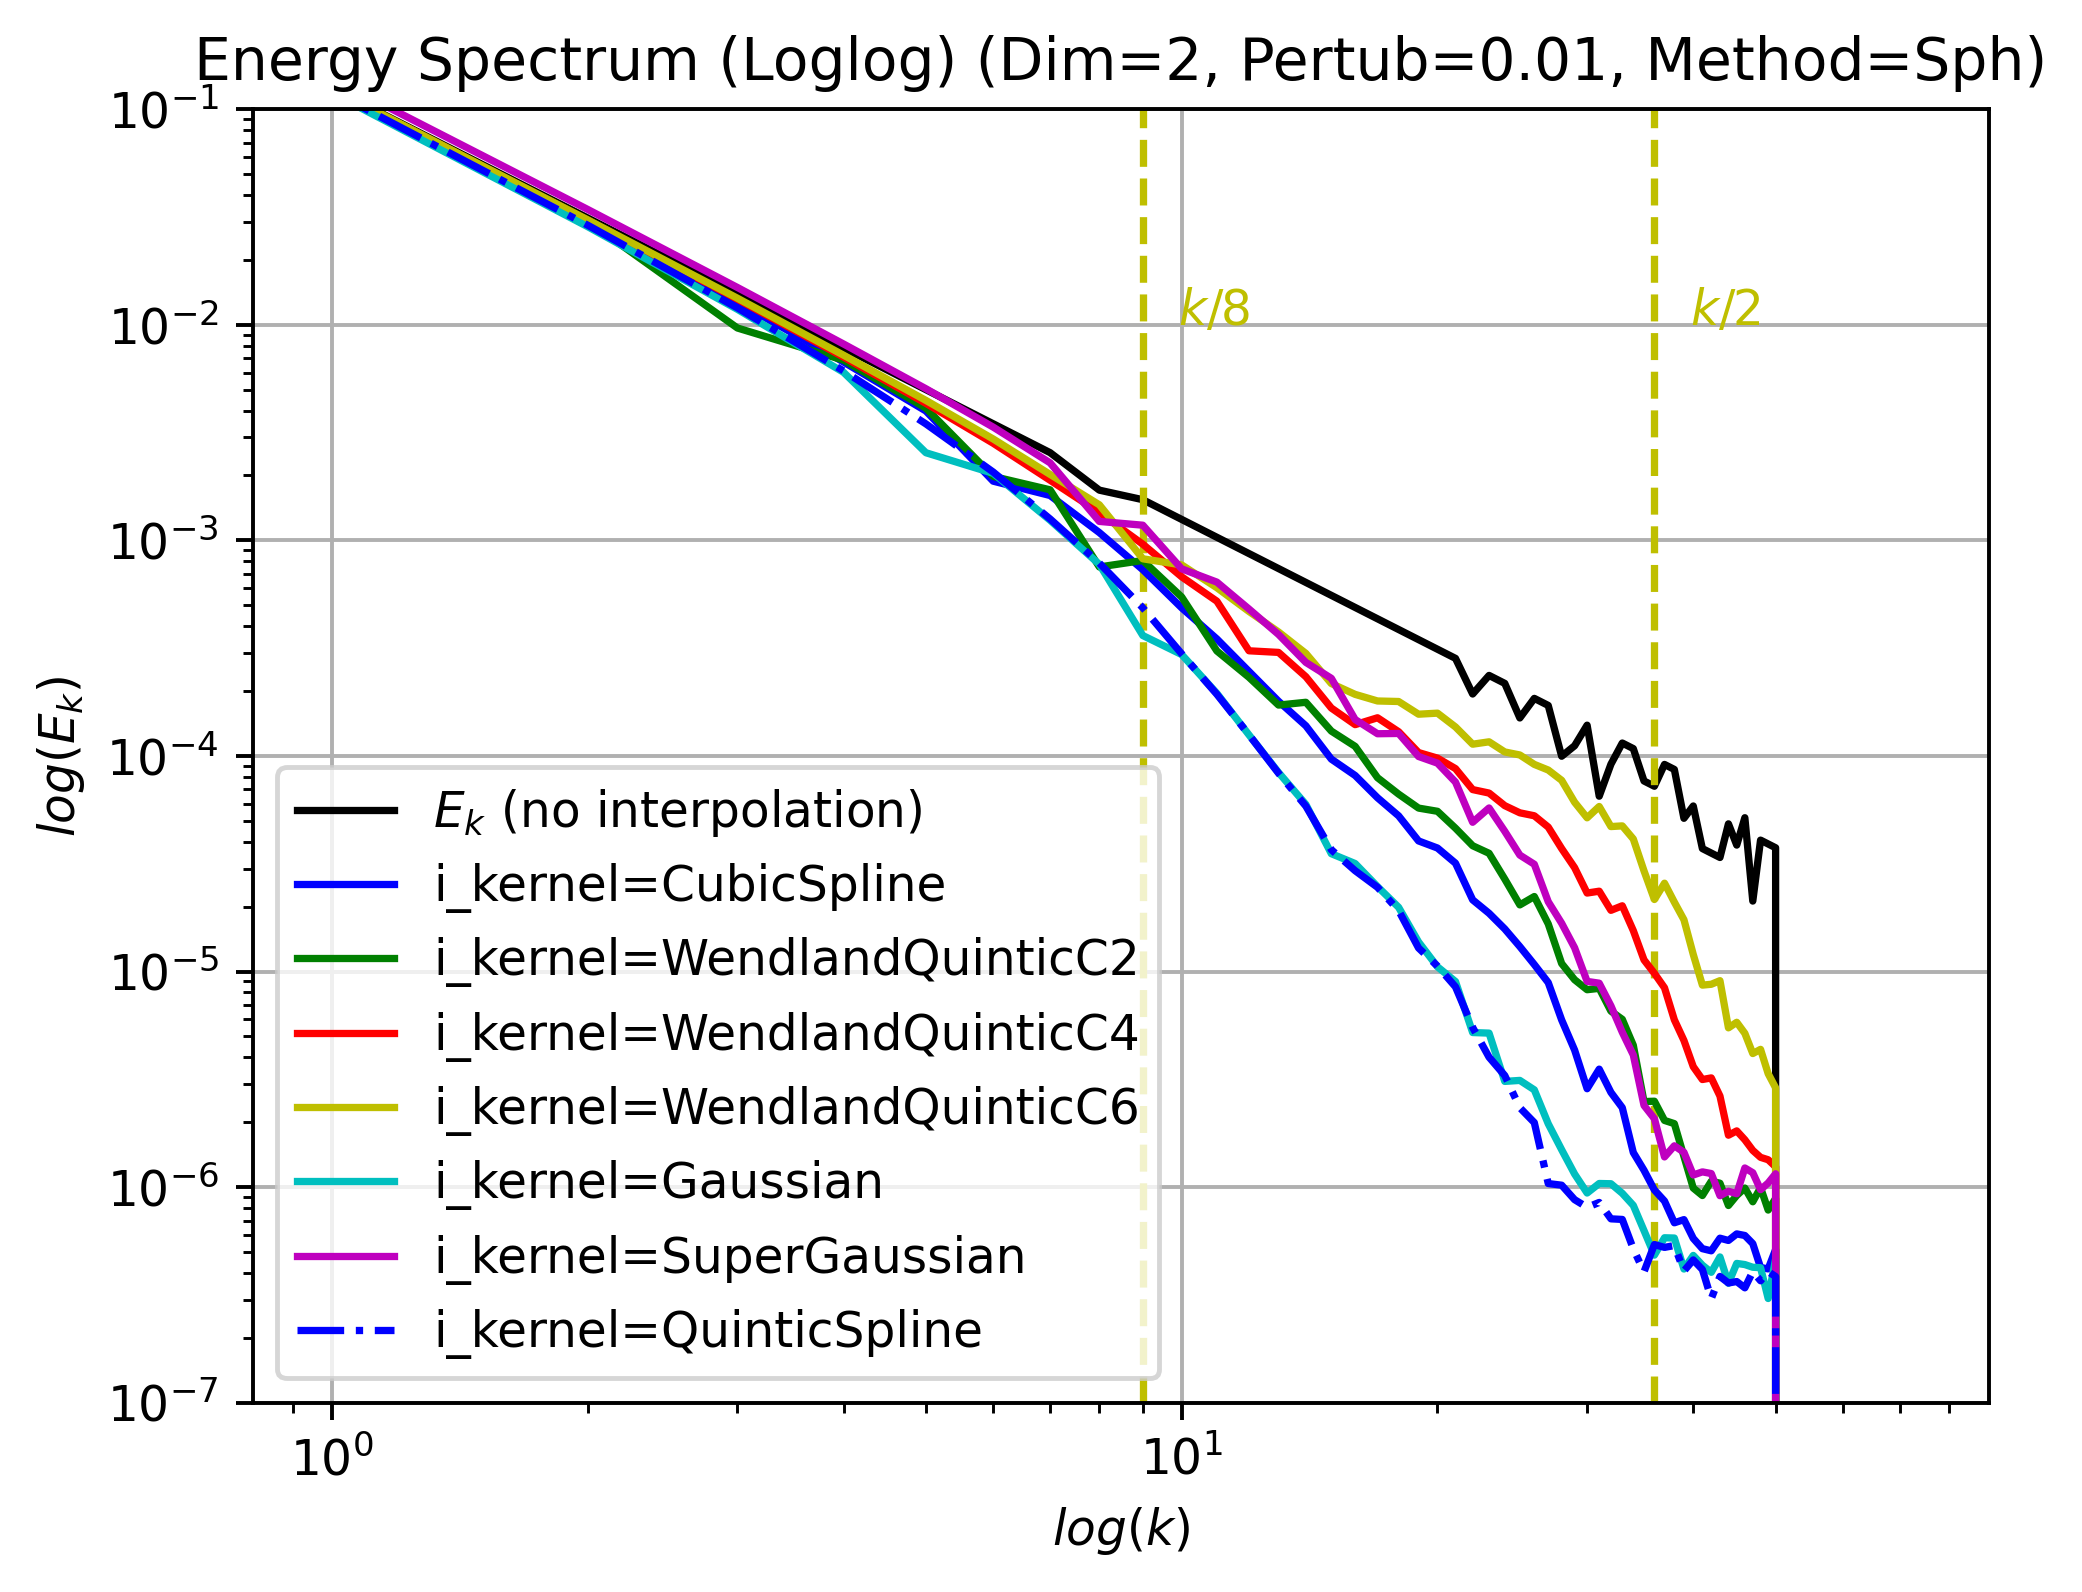
\includegraphics[width=6cm]{Code-Figures/sin-vel-prof-i-kernel/Energy Spectrum (Loglog) (Dim=2, Pertub=0.01, Method=Sph).png}
		\caption{$2D$ $E(k)$ field}
	\end{subfigure}
	\begin{subfigure}{7cm}
		\centering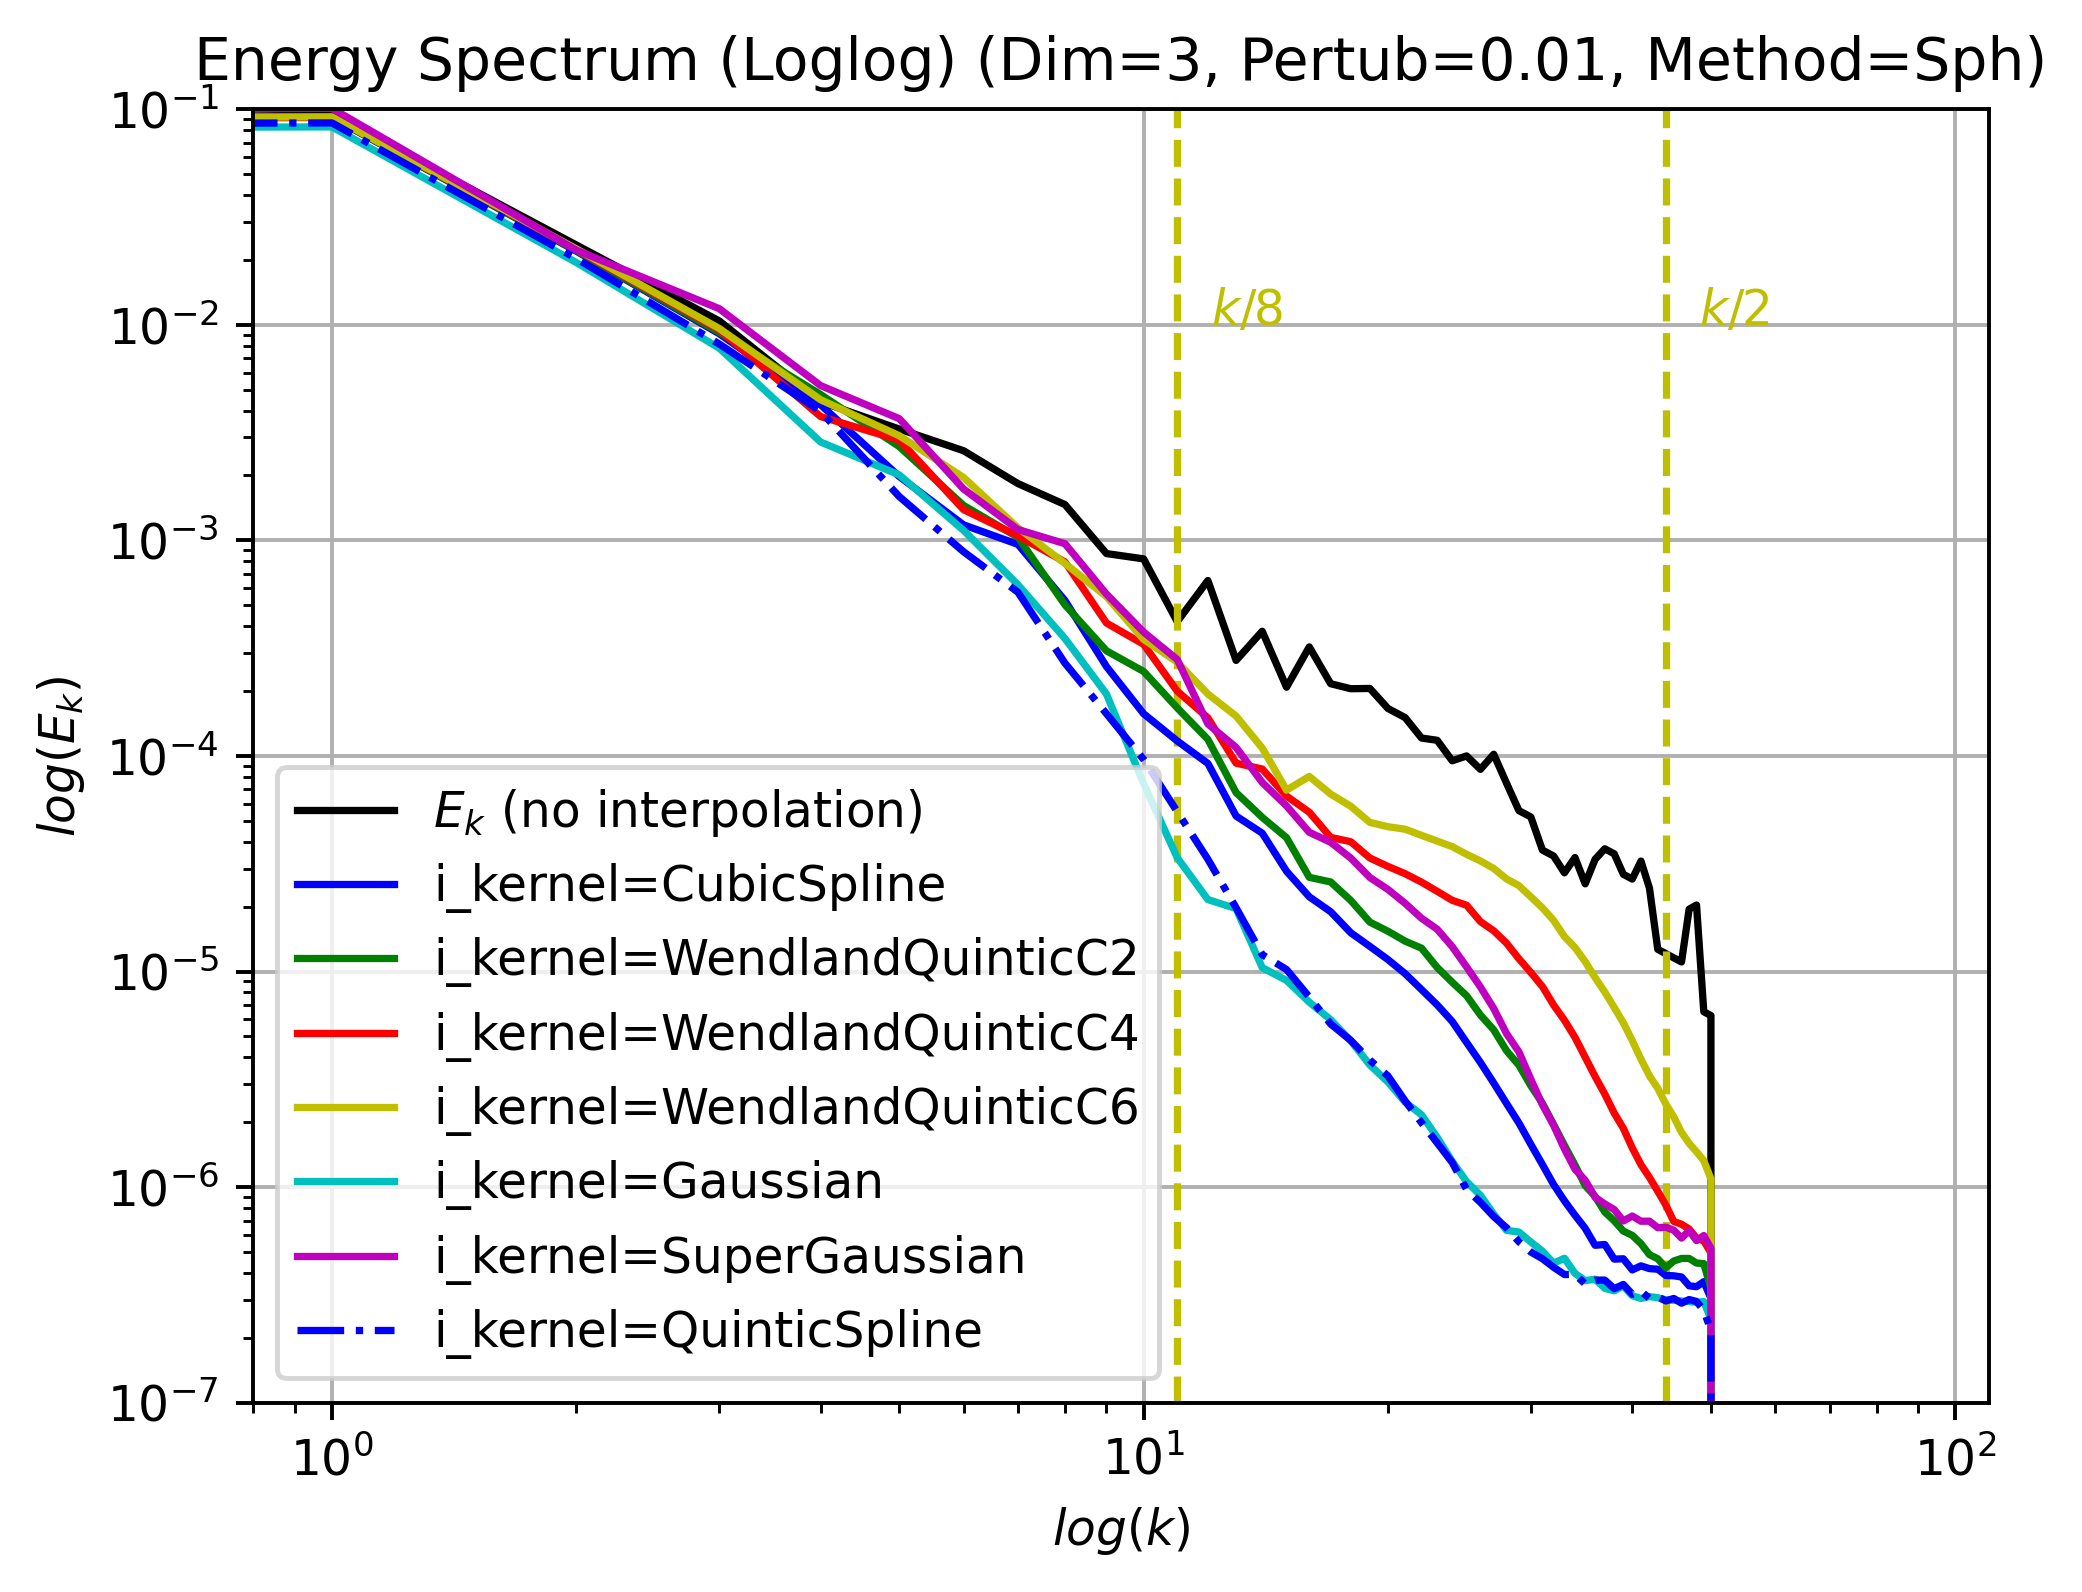
\includegraphics[width=6cm]{Code-Figures/sin-vel-prof-i-kernel/Energy Spectrum (Loglog) (Dim=3, Pertub=0.01, Method=Sph).png}
		\caption{$3D$ $E(k)$ field}
	\end{subfigure}
	\caption{The scalar fields $E(k)$ for $1D$, $2D$, and $3D$ case, for various interpolation kernels.}
	\label{fig:espec-scalar-fields-i-kernels}
\end{figure}

Finally, in order to measure the effect of particle resolution on the computed energy spectrum, test-cases with a $\gamma=1$ and $N=30$ were considered for all dimensions, with the range of number of particles along each axis being $[61, 91, 121]$.
From the results shown in \figref{fig:espec-scalar-fields-res}, it can be observed that the energy spectrum computed for the highest resolution, is observed to be the closest to the exact trend, for all dimensions.

\begin{figure}[htb!]
	\begin{subfigure}{7cm}
		\centering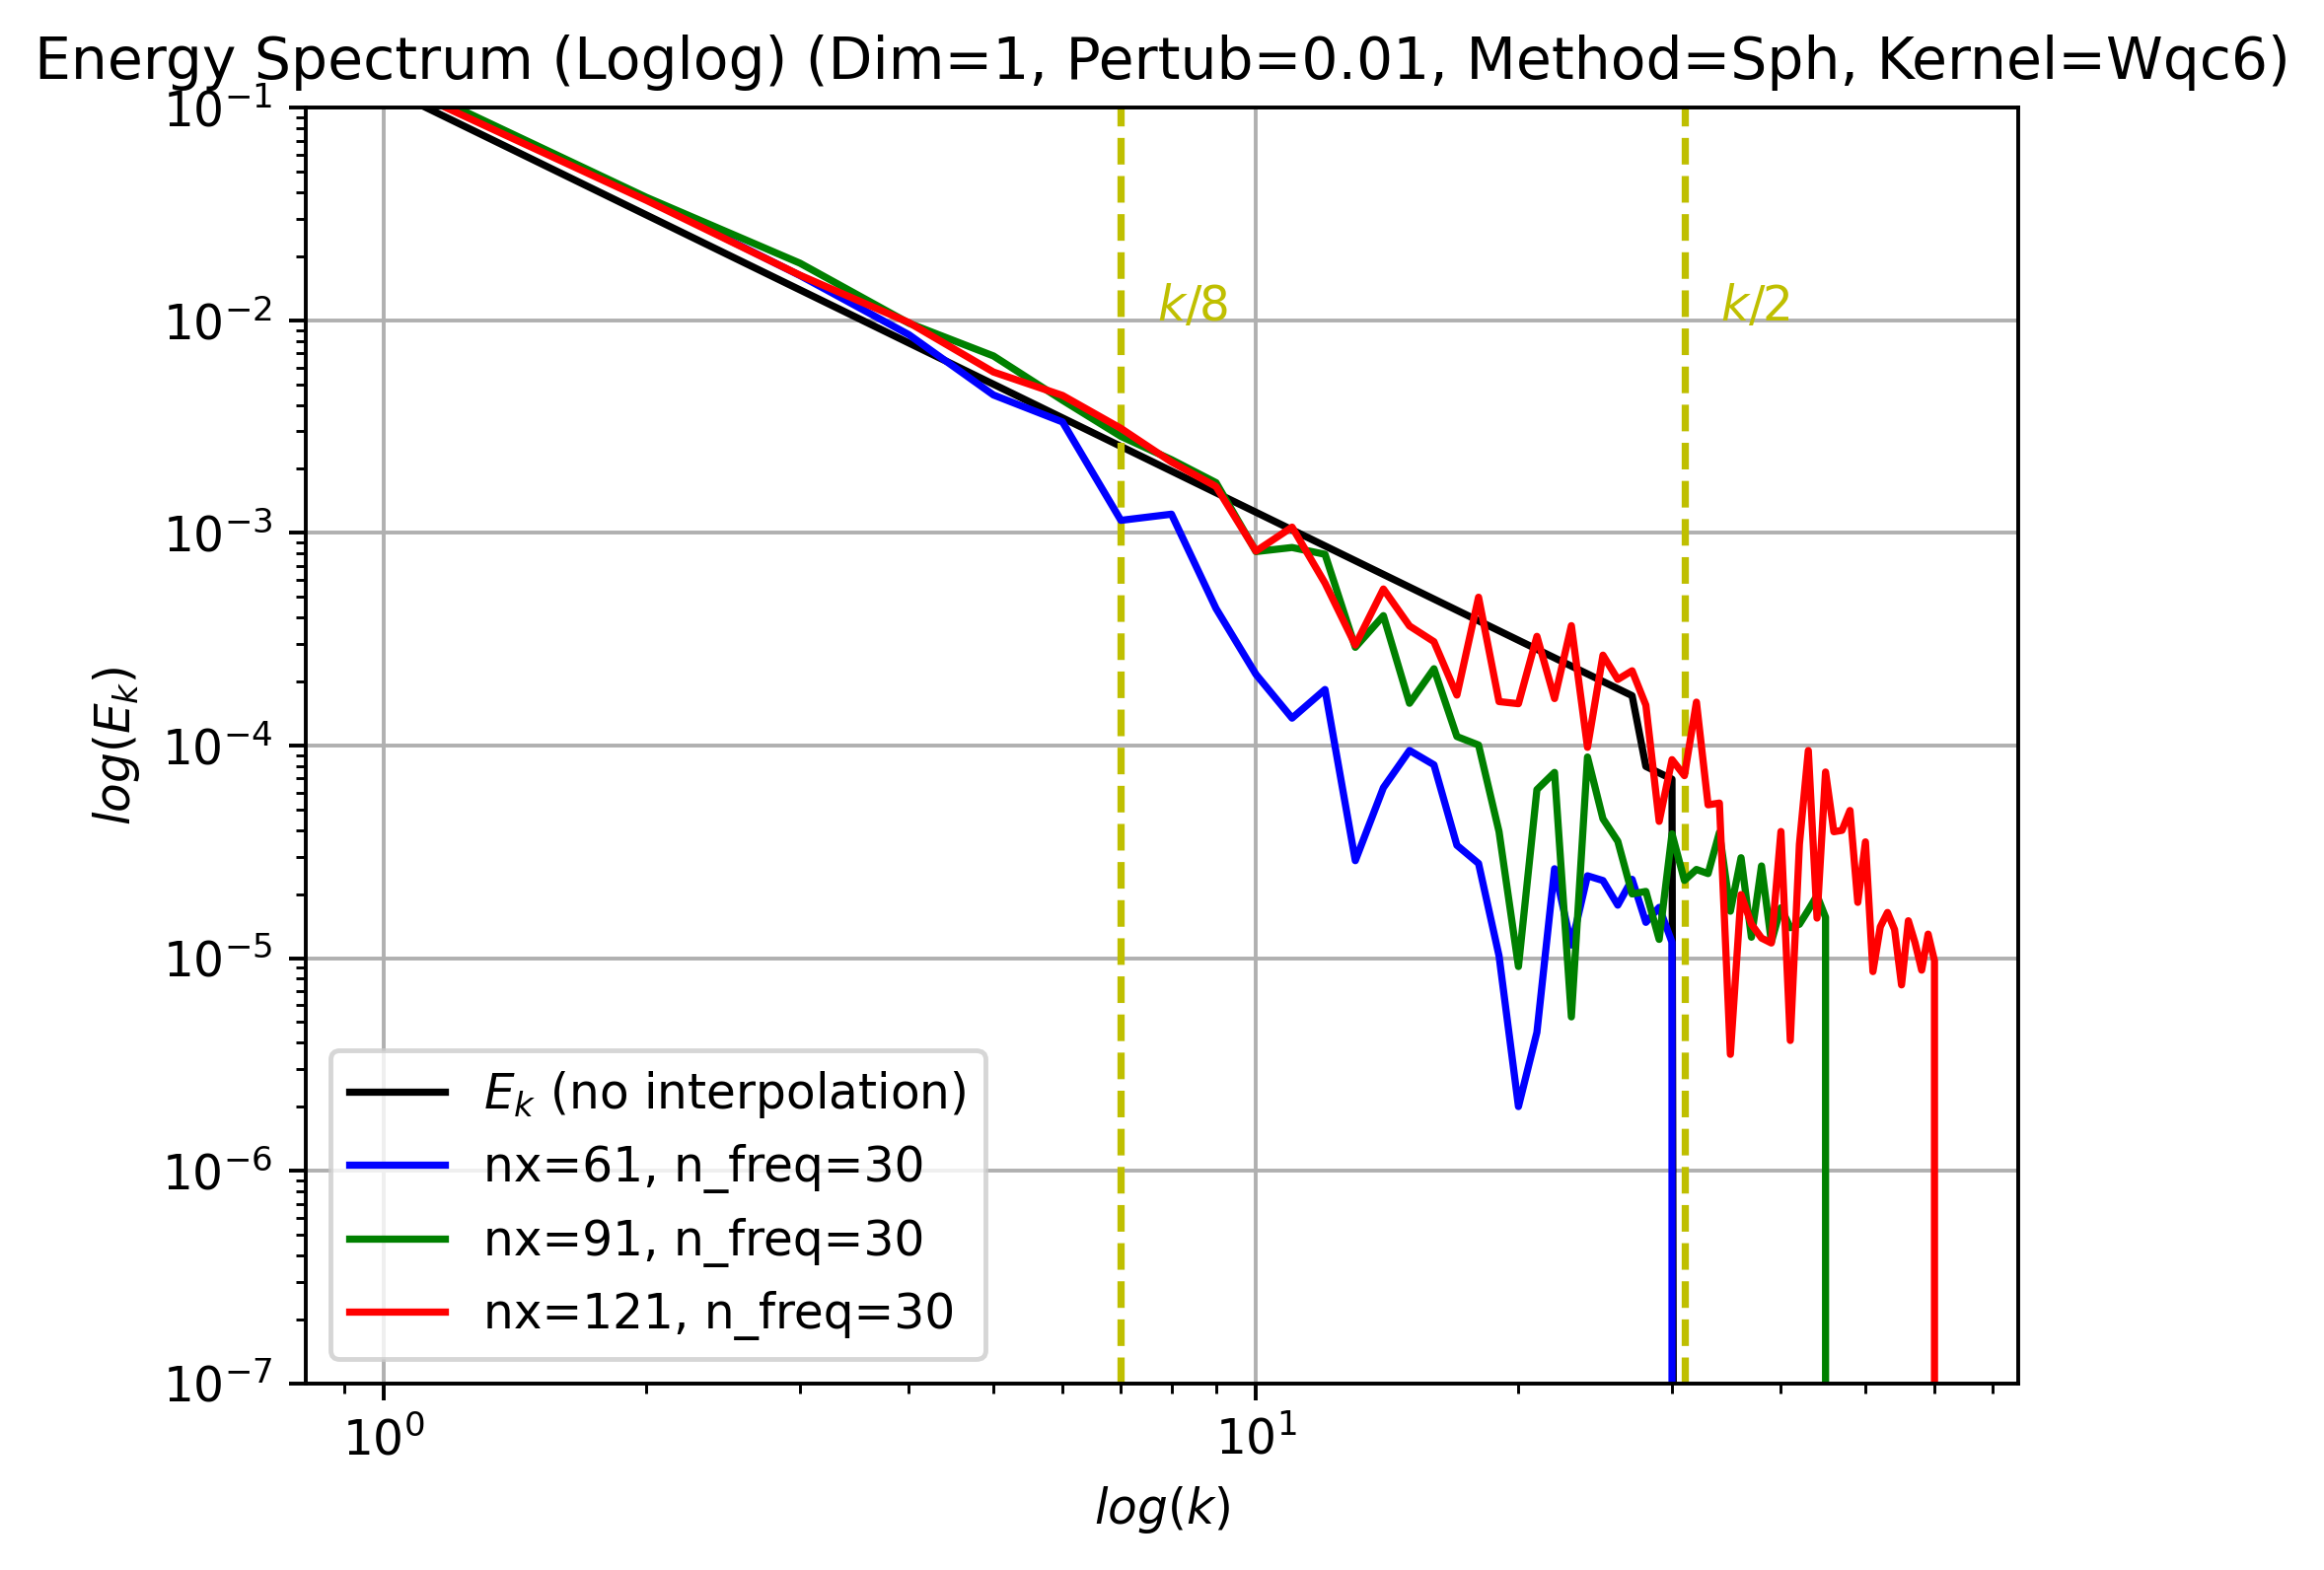
\includegraphics[width=6cm]{Code-Figures/sin-vel-prof-res/Energy Spectrum (Loglog) (Dim=1, Pertub=0.01, Method=Sph, Kernel=Wqc6).png}
		\caption{$1D$ $E(k)$ field}
	\end{subfigure}
	\begin{subfigure}{7cm}
		\centering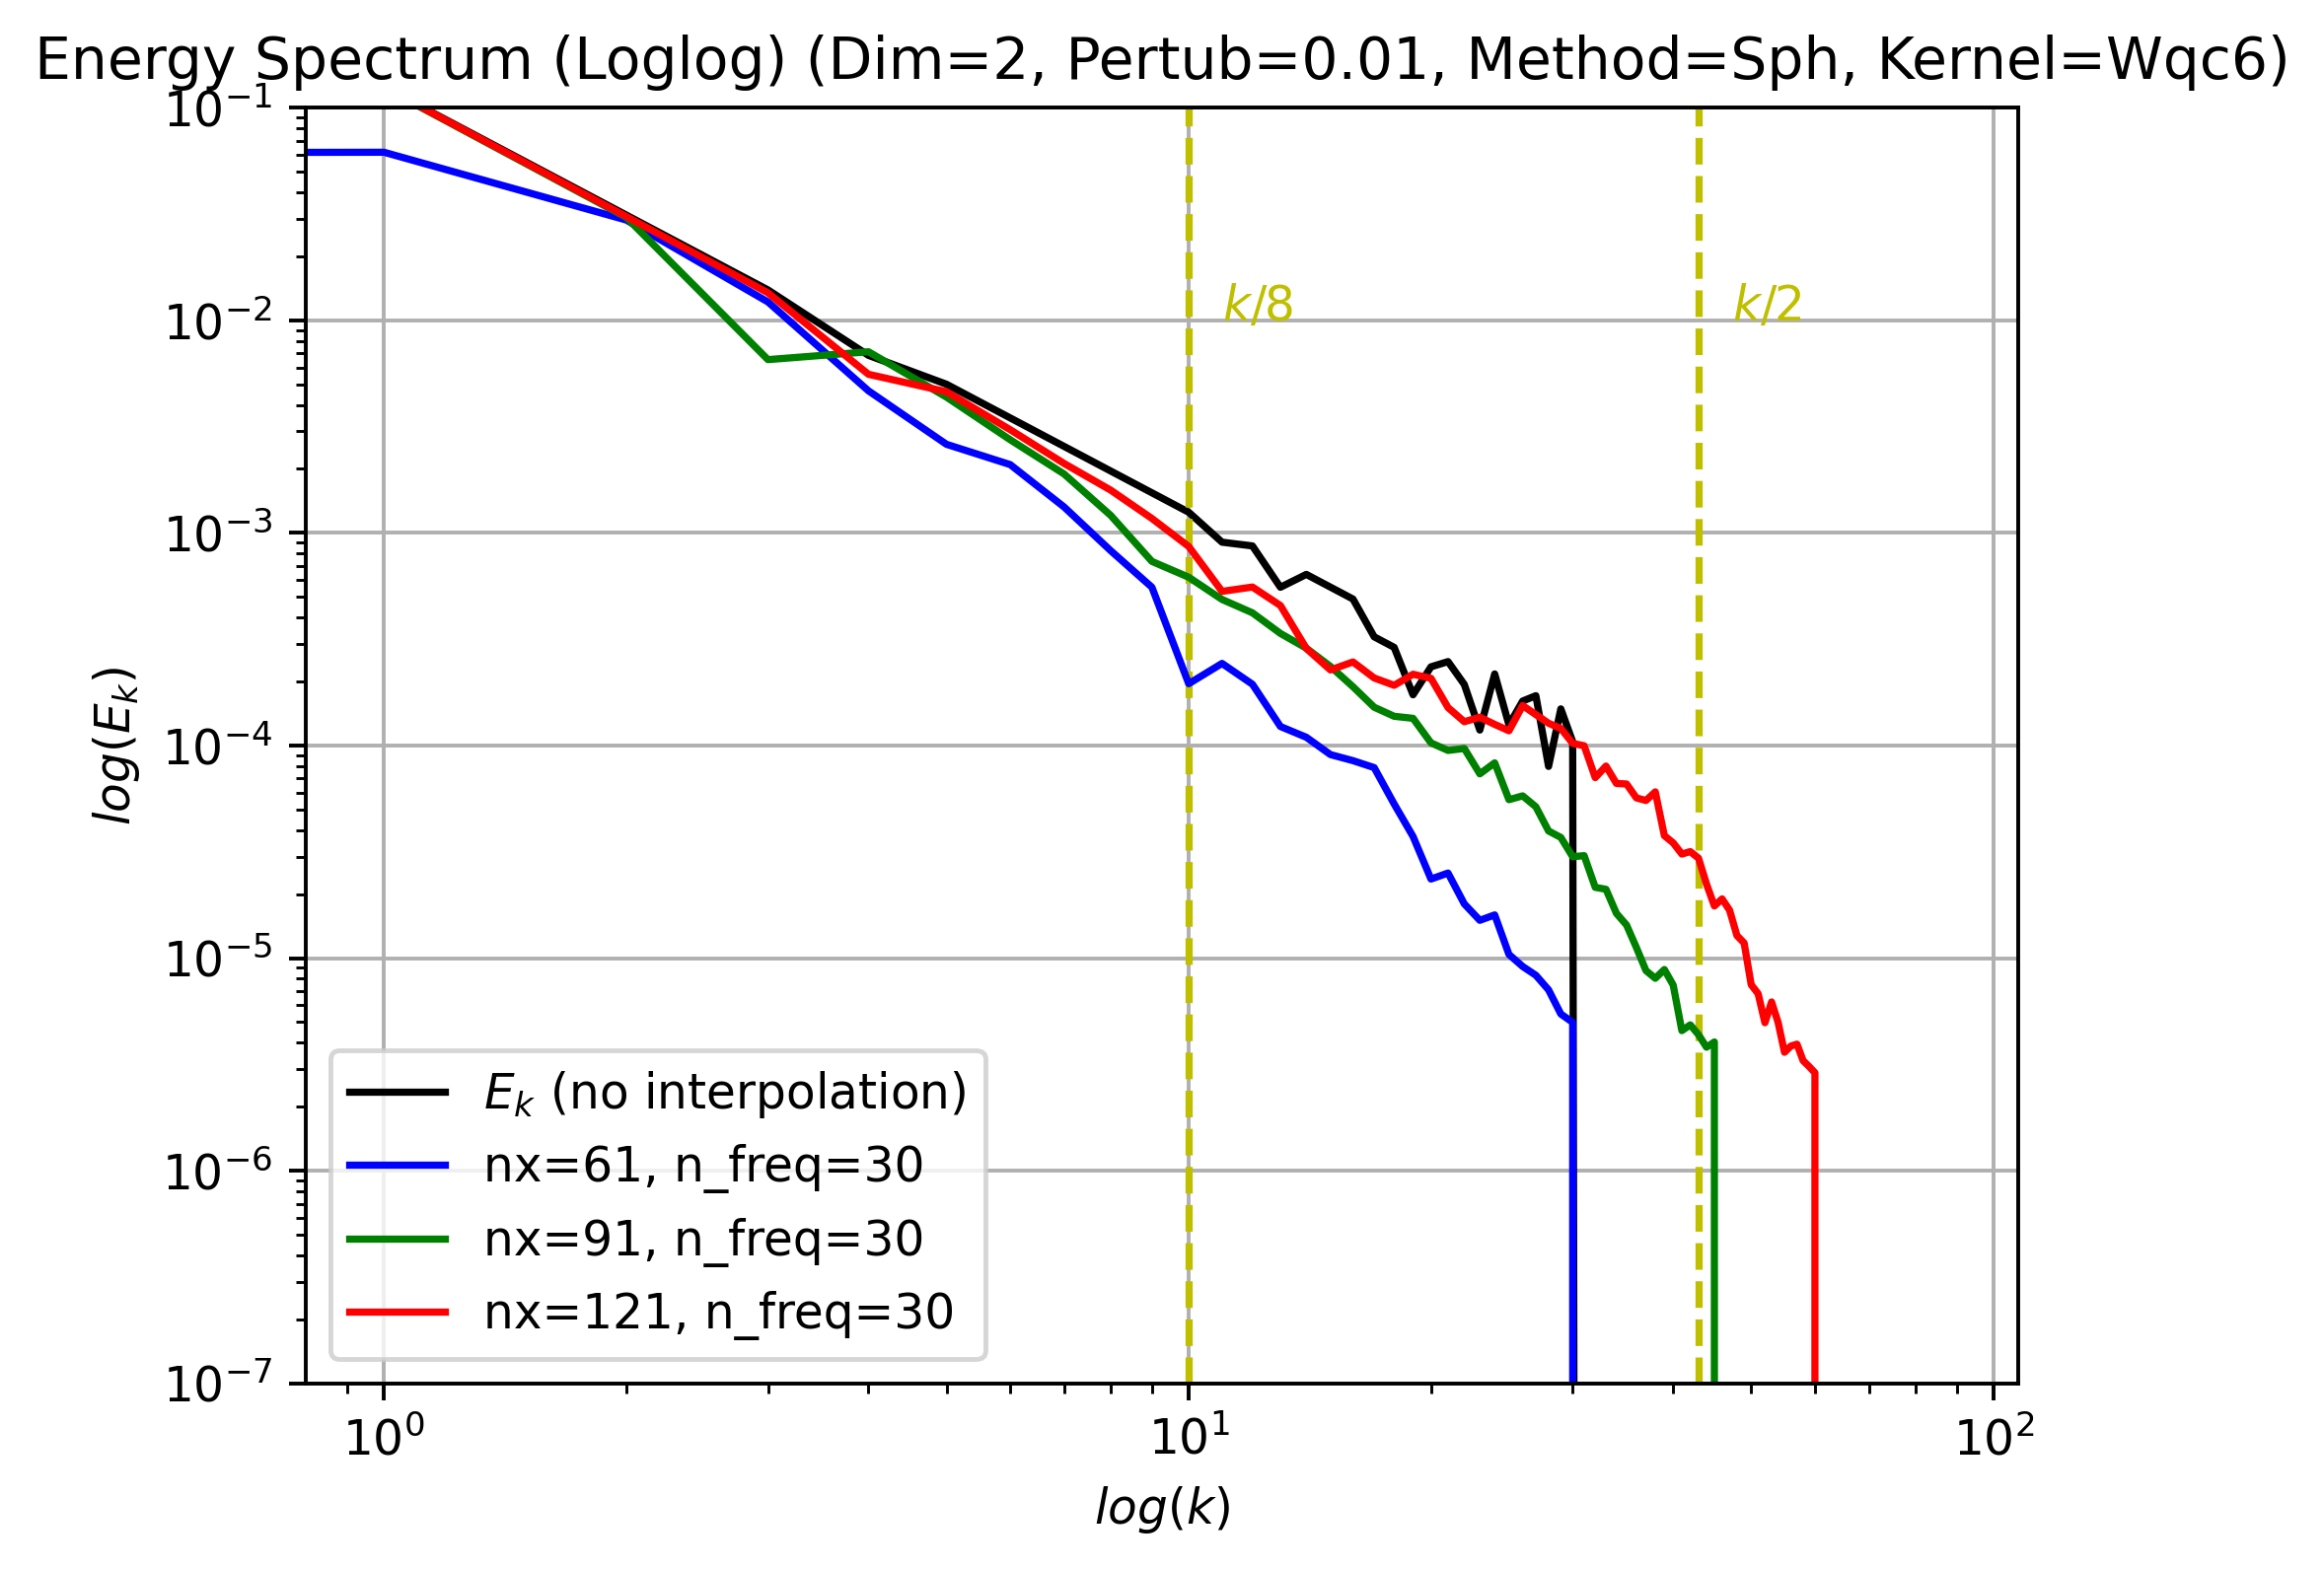
\includegraphics[width=6cm]{Code-Figures/sin-vel-prof-res/Energy Spectrum (Loglog) (Dim=2, Pertub=0.01, Method=Sph, Kernel=Wqc6).png}
		\caption{$2D$ $E(k)$ field}
	\end{subfigure}
	\begin{subfigure}{7cm}
		\centering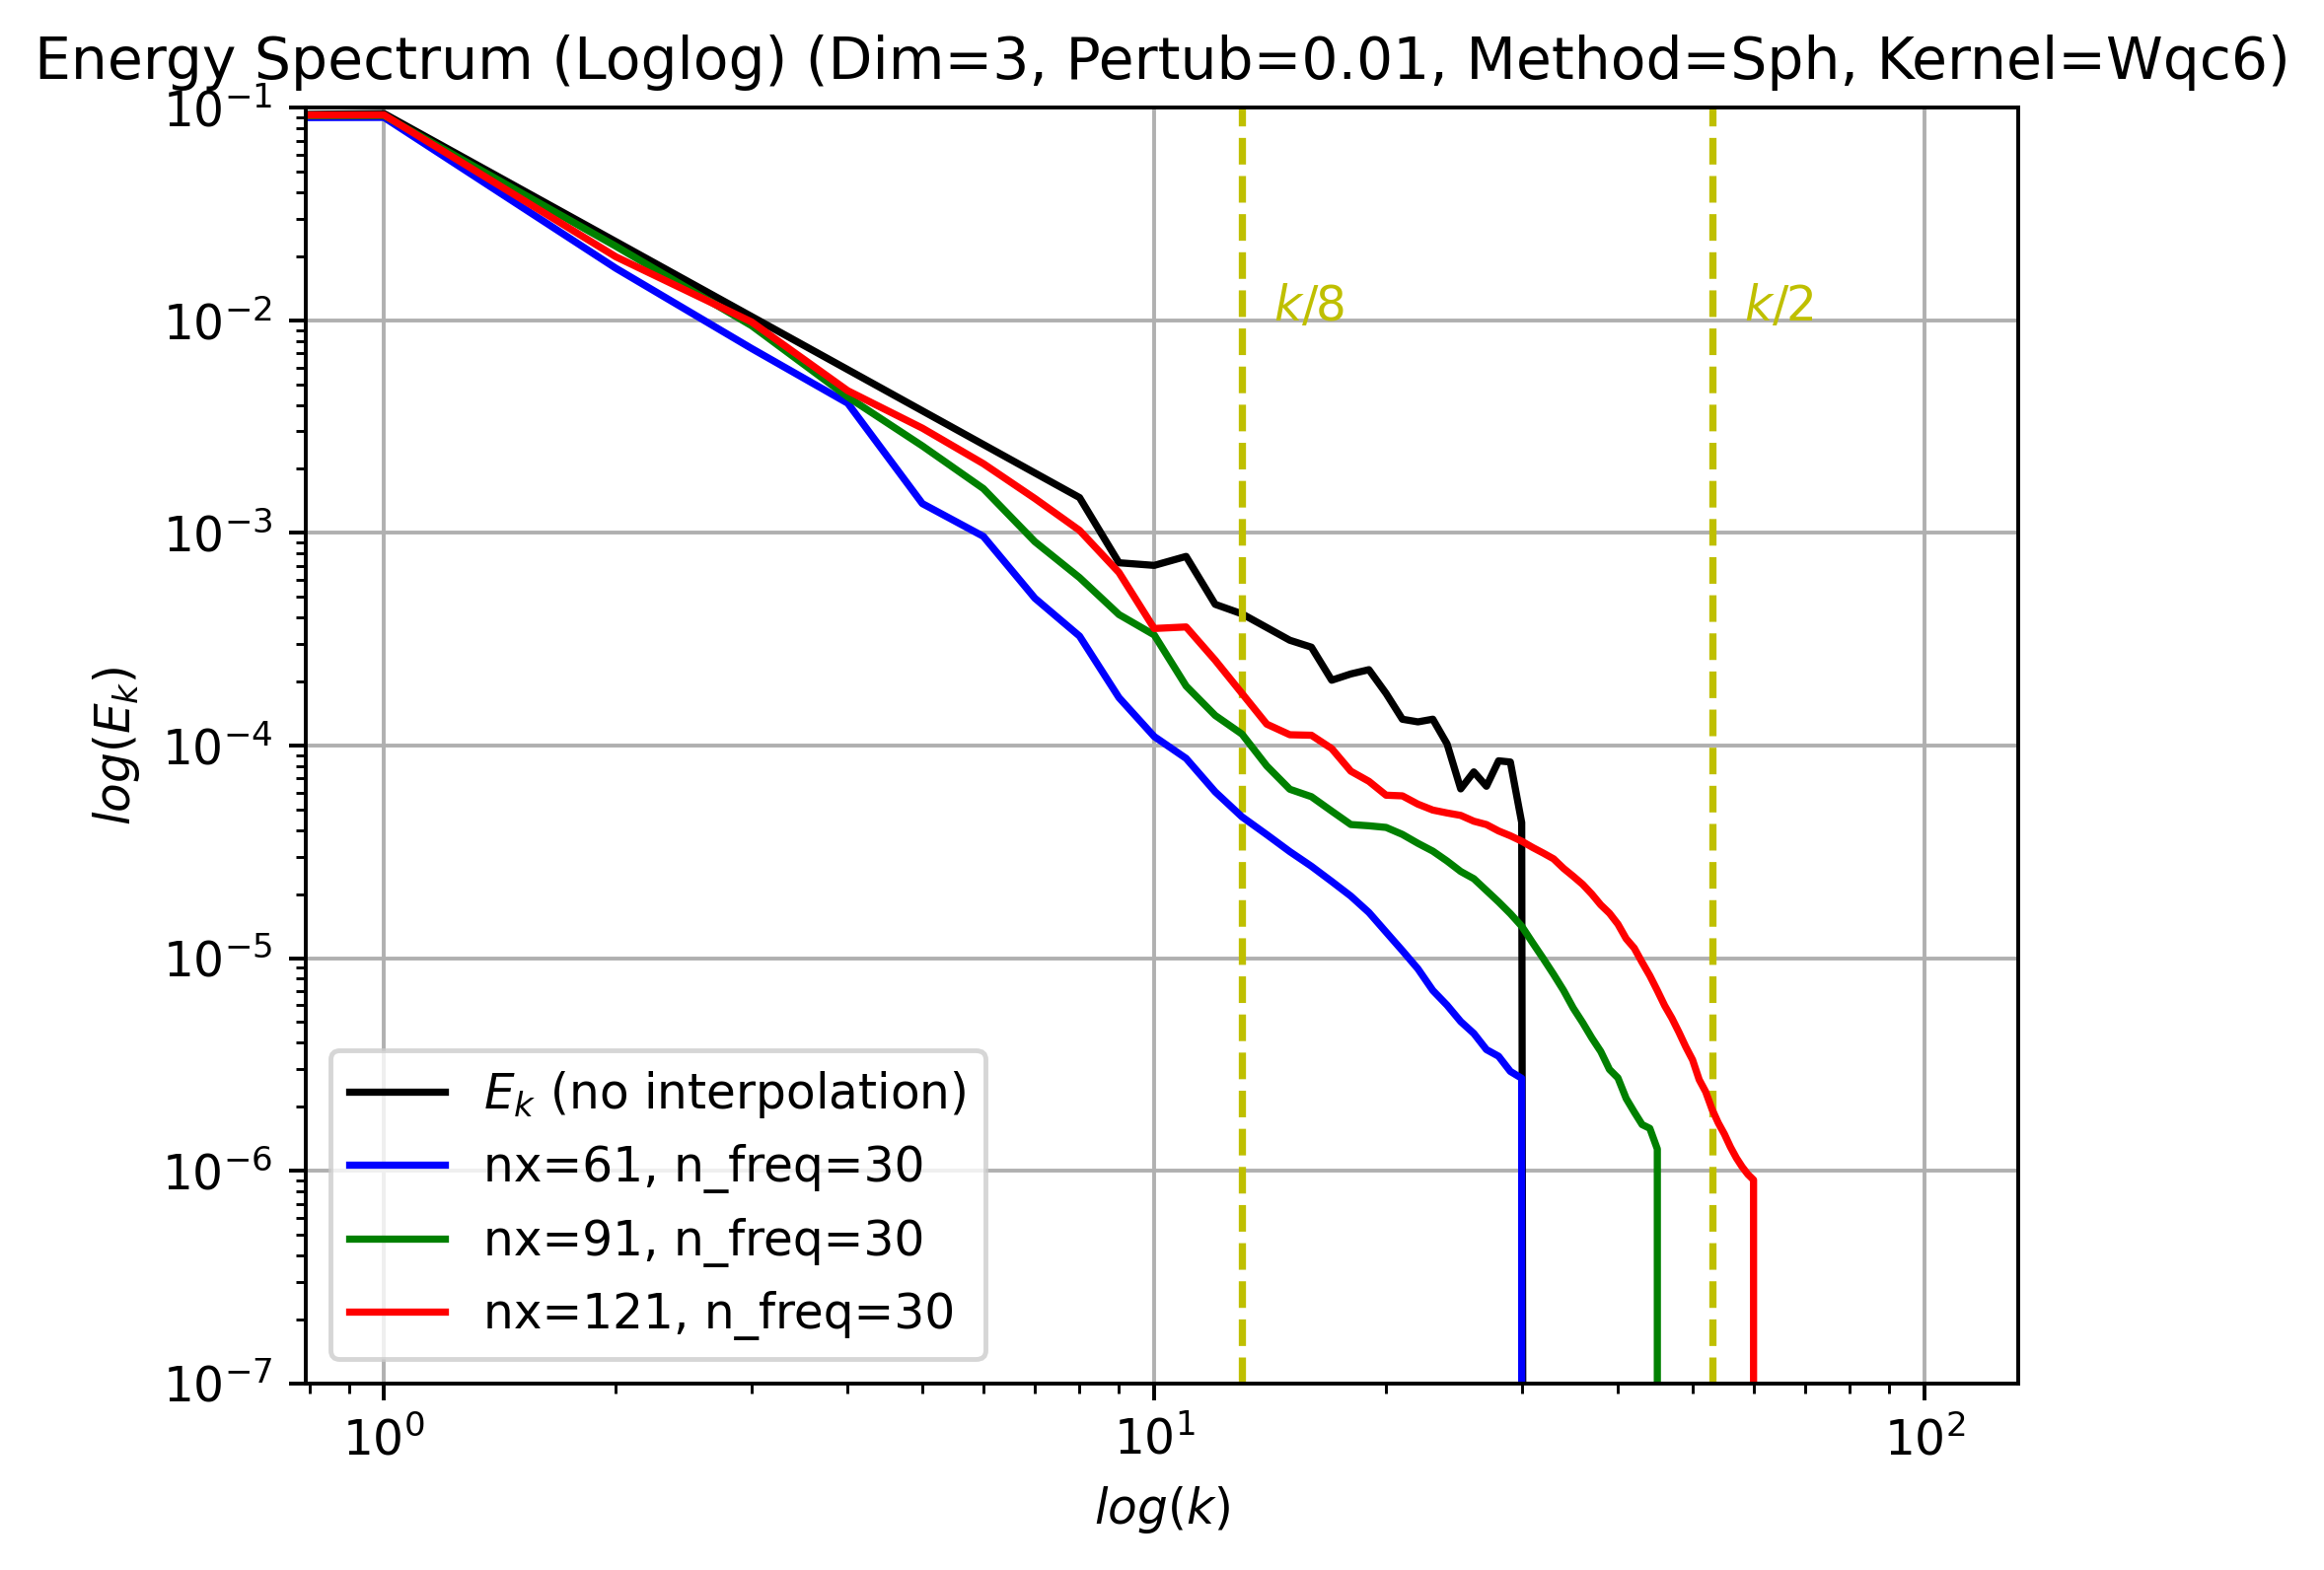
\includegraphics[width=6cm]{Code-Figures/sin-vel-prof-res/Energy Spectrum (Loglog) (Dim=3, Pertub=0.01, Method=Sph, Kernel=Wqc6).png}
		\caption{$3D$ $E(k)$ field}
	\end{subfigure}
	\caption{The scalar fields $E(k)$ for $1D$, $2D$, and $3D$ case, for various particle resolutions.}
	\label{fig:espec-scalar-fields-res}
\end{figure}


\subsection{Finite-time Lyapunov Exponent (FTLE) Field}

In order to compute the FTLE field, the flow field, at two different time instances is required, i.e., $t_i$ and $t_f$.
The flow field corresponding to the earlier time instance is stored in the \texttt{initial} particle array, while the flow field corresponding to the later time instance is stored in the \texttt{final} particle array.

The forward-in-time (FIT) FTLE field is calculated as defined in the work of \cite{sun2016detection}:
\begin{equation}
	\lambda_{t_i}^{t_f}(\vect{x}) = \frac{1}{\abs{t_f - t_i}} \ln \bigg( \sqrt{\Lambda_{max}[ \mathbb{C}_{t_i}^{t_f}(\vect{x}) ]}  \bigg),
\end{equation}
\begin{equation}
  \mathbb{C}_{t_i}^{t_f}(\vect{x}) = \mathbb{F}_{t_i}^{t_f}(\vect{x})^T \mathbb{F}_{t_i}^{t_f}(\vect{x}),
\end{equation}
where, $\mathbb{F}_{t_i}^{t_f}(\vect{x})$ is the deformation gradient tensor, and $\Lambda_{max}$ is the maximum eigenvalue of the Cauchy-Green tensor $\mathbb{C}_{t_i}^{t_f}(\vect{x})$. Correspondingly, the backward-in-time (BIT) FTLE field is calculated as:
\begin{equation}
  \lambda_{t_f}^{t_i}(\vect{x}) = \frac{1}{\abs{t_f - t_i}} \ln \bigg( \sqrt{ \frac{1}{\Lambda_{min}[ \mathbb{C}_{t_i}^{t_f}(\vect{x}) ]} }  \bigg).
\end{equation}

The corresponding, SPH approximations for the above equations are:
\begin{equation}
  \mathbb{F}_{t_i}^{t_f}(\vect{x}_i) = \sum_{j} \frac{m_j}{\rho_j} \vect{X}_{ji} \otimes \nabla \mathbb{L}( \vect{x}_i ) \DWIJ,
\end{equation}
\begin{equation}
  \mathbb{L}( \vect{x}_i ) = \bigg[ \sum_j \vect{x}_{ji} \otimes \nabla_i W(\abs{\vect{X}_{ji}}, h_i) \bigg]^{-1},
\end{equation}
where, $(\vect{x}_i, \vect{X}_i)$ corresponds to the initial and final position of the same particle.

In order to test the correctness of the FTLE field computation, the following test-cases were devised.
\begin{itemize}
  \item \texttt{parabolic}
  \begin{equation}
    X = 1.5x, \quad Y = x^2 + y,
  \end{equation}

  \item \texttt{spiral}
  \begin{equation}
    X = x + 0.1 \cos(2 \pi r^2), \quad Y = y + 0.1 \sin(2 \pi r^2), \quad r = \sqrt{x^2 + y^2},
    \end{equation}
\end{itemize}

\begin{figure}[htb!]
		\centering\includegraphics[width=10cm]{Code-Figures/ftle_parabolic.png}
		\caption{Parabolic displacement field}
    \label{fig:ftle-parabolic}
\end{figure}
\begin{figure}[htb!]
  \centering\includegraphics[width=10cm]{Code-Figures/ftle_spiral.png}
  \caption{Spiral displacement field}
  \label{fig:ftle-spiral}
\end{figure}

As seen in \figref{fig:ftle-parabolic} and \figref{fig:ftle-spiral} ($B_0$: initial configuration, $B_t$: final configuration), it can be observed that although the FTLE fields can to an extent qualitatively capture the evolution of the configurations, i.e, attracting/repelling pathlines, it is however, not as accurate in terms of actually capturing the exact pathlines. Therefore, it was concluded that in-place of FTLE fields, tracer particles can be used to visualize the flow field, which would be more accurate in terms of capturing the exact pathlines, but would be computationally more expensive, since the tracer particles would have to be advected along with the flow field, and would also require additional post-processing to visualize the pathlines. They would also have to be done in-situ, i.e., during the simulation itself, as opposed to the FTLE fields, which can be computed post-simulation or in-situ as well.
% TODO: iPad fig of atracting and repelling pathlines


\section{Turbulence Modelling}
\subsection{Implementation of models}
A broad classification of the major categories of turbulence models, has already been discussed in \chapref{chap:turbulence-modelling}.
In order to better understand the nature of each major categories, and to subsequently understand the implementation of the same, a select few representative schemes from each of these models are considered, which are listed in \tabref{tab:rep-turb-models}.

\begin{table}[ht!]
  \centering
  \resizebox{\textwidth}{!}{%
  \begin{tabular}{|l|l|l|l|}
  \hline
  \multicolumn{1}{|c|}{\textbf{Turbulence Model}} & \multicolumn{1}{c|}{\textbf{Section}} & \multicolumn{1}{c|}{\textbf{Scheme Name}}                                                                               & \multicolumn{1}{c|}{\textbf{Reference}}  \\ \hline
  Viscosity-based Model                           & \secref{sec:visc-based-model}                  & \begin{tabular}[c]{@{}l@{}}Lagrangian with iterative PST and \texttt{coupled\_c} viscosity formulation\\ (L-IPST-C)\end{tabular} & \cite{Negi2022Techniques}            \\ \hline
  Large Eddy Simulation-based Model               & \secref{sec:les-based-model}                   & SPH-LES                                                                                                                          & \cite{Okraschevski2022}              \\ \hline
  Lagrangian LES-based Model                      & \secref{sec:lagrangian-les-based-model}        & $\delta$-LES-SPH                                                                                                                 & \cite{Colagrossi2021QuasiLagrangian} \\ \hline
  RANS-based k-epsilon Model                      & \secref{sec:rans-based-k-epsilon-model}        & $k-\epsilon$ SPH                                                                                                                 & \cite{Shao2006}                      \\ \hline
  LANS-based Model                                & \secref{sec:lans-based-model}                  & SPH-$\epsilon$                                                                                                                   & \cite{Monaghan2017}                  \\ \hline
  \end{tabular}%
  }
  \caption{Implementation of representative turbulence models.}
  \label{tab:rep-turb-models}
\end{table}

In order to test the schemes for SOC, the Taylor-Green vortex problem is chosen. The test-cases are coded using \texttt{automan} \parencite{RamachandranAutoman2018}, which is an open source, Python-based automation framework. All of the simulations run hereafter, are run upto a final time of $t_f=0.1$, with the resolution for each run consisting of $N=[25^2, 50^2, 100^2]$ particles respectively, with the Reynolds number ranging between $Re=[100, 1000, 10000]$ respectively. All of the simulations are run using the \texttt{WendlandQuinticC4} kernel, with a radius multiplier of $2.0$. This choice was based on the work of \cite{Negi2022Techniques}.

The $L_1$ error for each simulation in a run is computed, and plotted against the inverse of the particle spacing, in order to ascertain the order of convergence (OOC) of the scheme. The $L_1$ error at a given time instance is computed as:
\begin{equation}
  L_1(t) = \frac{mean{\abs{\vect{v}^2(t) - \vect{v}^2_{exact}(t)}}}{mean{\abs{\vect{v}^2_{exact}(t)}}},
\end{equation}
where, $\vect{v}(t)$ is the velocity field at time $t$, and $\vect{v}_{exact}(t)$ is the exact velocity field at time $t$.
Subsequently, the $L_1$ error for the entire simulation, is defined as the mean over all the time instances, i.e.,
\begin{equation}
  L_1 = \frac{1}{n_t} \sum_{i=1}^{n_t} L_1(t_i).
\end{equation}

\subsection{L-IPST-C Scheme}

The L-IPST-C scheme was considered over the other viscosity-based schemes, since it was observed to be actually second-order convergent (SOC) by \cite{Negi2022Techniques}, for a wide variety of problems, which included the Gresho vortex problem, Kelvin-Helmholtz instability problem, and the Taylor-Green vortex problem. This scheme considers the weakly-compressible NS equations as the governing equations, and uses the \texttt{coupled\_c} viscosity formulation, which is corrected using the Bonet and Lok correction \parencite{bonet1999variational}. Hence, since the scheme by definition has the viscous term in its governing equation, it does require any additional `artificial'-viscosity term to be added.
The scheme also incorporates the iterative particle shifting technique (IPST) by \cite{Huang_Long_Li_Liu_2019}, in order to redistribute the particles to obtain a reasonably uniform grid of particles in the domain. Besides shifting the position of the particles, the scheme also updates particles' properties such as the density and velocity to keep the approximation of the particle $O(h^2)$.
Based on the parametric study conducted by \cite{Negi2022Techniques}, the proposed scheme is observed to be SOC, by considering the the speed of sound to be $c_s = 20$, and the shifting frequency for the particles through PST to be at every 10 iterations $f_{pst} = 10$.

Since, the study dealt with problems of low $Re$, the scheme was tested for various time-integration schemes from the Runge-Kutta family of integrators, in order to identify their effects, and to subsequently identify the most suitable integrator for problems of high $Re$.
The integrators considered were:
\begin{itemize}
  \item Predict-Evaluate-Correct (\texttt{PEC}),
  \item Runge-Kutta 2 (\texttt{RK2}),
  \item Runge-Kutta 2 with adaptive time-step (\texttt{RK2 Adaptive}),
  \item Runge-Kutta 3 (\texttt{RK3}), and
  \item Runge-Kutta 4 (\texttt{RK4}),
\end{itemize}
with a corresponding $CFL$ values of $[1, 1, 1.5, 2, 2]$ respectively.

\begin{figure}[htb!]
  \begin{subfigure}{7cm}
    \centering\includegraphics[width=6cm]{Code-Figures/lipstc/integrator/dt_pois_conv_c0_20_re_100.png}
    \caption{$Re = 100$}
  \end{subfigure}
  \begin{subfigure}{7cm}
    \centering\includegraphics[width=6cm]{Code-Figures/lipstc/integrator/dt_pois_conv_c0_20_re_1000.png}
    \caption{$Re = 1000$}
  \end{subfigure}
  \begin{subfigure}{7cm}
    \centering\includegraphics[width=6cm]{Code-Figures/lipstc/integrator/dt_pois_conv_c0_20_re_10000.png}
    \caption{$Re = 10000$}
  \end{subfigure}
  \caption{Convergence of the L-IPST-C scheme for various time-integration schemes.}
  \label{fig:lipstc-integrator}
\end{figure}

From the results shown in \figref{fig:lipstc-integrator}, it is evident that the order of the integrator does not appear to have much effect on the OOC, and almost negligible effect on the actual magnitude of the $L_1$ errors as well.
This seems to highlight a much more important aspect of the effect and role of time-integration schemes in SPH in general, which is that the time-step size is the most important factor, and the order of the integrator is not as important, since the time-step size is typically chosen to be small enough to ensure stability, and hence, the error introduced by the time-integration scheme is typically negligible.

Also, when the run-times of these integrators were analysed, the higher order integrators are observed to be more computationally expensive, allowing for the \texttt{PEC} integrator to be around $\approx 1.6\times$ faster, which is reflected in the run-times shown in \figref{fig:lipstc-integrator-rt}.
Typically such higher order integrators can be used with much larger $CFL$ values, allowing for larger time-steps and consequently faster run-times. However, in the case of SPH, such generalisations cannot be made, since the stability of the scheme is not only dependent on the time-step size, but also on the particle spacing, and hence, the $CFL$ value is typically chosen to be close to $1.0-2.0$.
Therefore, the \texttt{PEC} integrator is chosen as the default integrator for the L-IPST-C scheme.

\begin{figure}[htb!]
  \begin{subfigure}{7cm}
    \centering\includegraphics[width=6cm]{Code-Figures/lipstc/integrator/pois_rt_pst_10_c0_20_re_100.png}
    \caption{$Re = 100$}
  \end{subfigure}
  \begin{subfigure}{7cm}
    \centering\includegraphics[width=6cm]{Code-Figures/lipstc/integrator/pois_rt_pst_10_c0_20_re_1000.png}
    \caption{$Re = 1000$}
  \end{subfigure}
  \begin{subfigure}{7cm}
    \centering\includegraphics[width=6cm]{Code-Figures/lipstc/integrator/pois_rt_pst_10_c0_20_re_10000.png}
    \caption{$Re = 10000$}
  \end{subfigure}
  \caption{Run-time (in $s$) of the L-IPST-C scheme for various time-integration schemes.}
  \label{fig:lipstc-integrator-rt}
\end{figure}


\subsection{SPH-LES Scheme}
The SPH-LES scheme was considered over the other LES-based schemes, since it was observed to be actually SOC by \cite{Okraschevski2022}, since the scheme they proposed utilised the compressible NS equations and subjected those to a spatial averageing operator to obtain the filtered governing equations. They also considered, three different models for the turbulent eddy viscosity, which included the standard Smagorinsky model, $\sigma$-model and the standard model discretised in the Monaghan-Cleary-Gingold (MCG) form (detailed in \secref{sec:Modified-Smagorinsky-Model}). Therefore, the model appeared comprehensive in terms of its implementation, and hence, was chosen, along with the \texttt{SMAG} model, which is the standard Smagorinsky model, since their study revealed that this model was the most accurate relatively in terms of its prediction of the energy spectrum, while using the \texttt{PEC} integrator.

\begin{figure}[htb!]
  \begin{subfigure}{7cm}
    \centering\includegraphics[width=6cm]{Code-Figures/okra2022/pst/dt_pois_conv_c0_20_re_100.png}
    \caption{$Re = 100$}
  \end{subfigure}
  \begin{subfigure}{7cm}
    \centering\includegraphics[width=6cm]{Code-Figures/okra2022/pst/dt_pois_conv_c0_20_re_1000.png}
    \caption{$Re = 1000$}
  \end{subfigure}
  \begin{subfigure}{7cm}
    \centering\includegraphics[width=6cm]{Code-Figures/okra2022/pst/dt_pois_conv_c0_20_re_10000.png}
    \caption{$Re = 10000$}
  \end{subfigure}
  \caption{Convergence of the SPH-LES scheme for various $f_{pst}$ values.}
  \label{fig:okra2022-pst}
\end{figure}


In order to identify the effects of the PST on the scheme, the following values were considered: $f_{pst} = [None, 10, 50, 100]$, with the speed of sound for the particles through PST to be $c_s = 20$. The results are shown in \figref{fig:okra2022-pst}, where it can be seen that the scheme worringly appears to be zero order convergent. To gain a better understanding of the forces, the velocity magnitude field and the energy spectrum were plotted.
In \figref{fig:okra2022-pst-vmag}, it can be observed that without PST, the particles get clustered, and there are marked regions which are devoid of particles. It is also evident, that high values of $f_{PST}$ are also not desirable, since it leads to the particles being clustered in a different manner, and also leads to the formation of void regions.
Also, in \figref{fig:okra2022-pst-espec}, it can be observed that the slope of the energy spectrum at the final time instance (yellow line), increases with increasing values of $f_{pst}$, which is indicative of the fact that the energy is being concentrated at the higher resolution scales, which is expected for the high $Re$ case.
Therefore, a value of $f_{pst} = 10$ is chosen as the default value for the PST.

\begin{figure}[htb!]
  \begin{subfigure}{7cm}
    \centering\includegraphics[width=6cm]{Code-Figures/okra2022/pst/c0_20_tait_pec_dtmul_1_nx_50_pst_-1_re_10000_ok2022/final_vmag.png}
    \caption{No PST}
  \end{subfigure}
  \begin{subfigure}{7cm}
    \centering\includegraphics[width=6cm]{Code-Figures/okra2022/pst/c0_20_tait_pec_dtmul_1_nx_50_pst_10_re_10000_ok2022/final_vmag.png}
    \caption{$f_{pst} = 10$}
  \end{subfigure}
  \begin{subfigure}{7cm}
    \centering\includegraphics[width=6cm]{Code-Figures/okra2022/pst/c0_20_tait_pec_dtmul_1_nx_50_pst_50_re_10000_ok2022/final_vmag.png}
    \caption{$f_{pst} = 50$}
  \end{subfigure}
  \begin{subfigure}{7cm}
    \centering\includegraphics[width=6cm]{Code-Figures/okra2022/pst/c0_20_tait_pec_dtmul_1_nx_50_pst_100_re_10000_ok2022/final_vmag.png}
    \caption{$f_{pst} = 100$}
  \end{subfigure}
  \caption{Velocity magnitude field for the SPH-LES scheme for various $f_{pst}$ values $(N=50^2, t_f=0.1, Re=10000, c_s=20)$.}
  \label{fig:okra2022-pst-vmag}
\end{figure}

\begin{figure}[htb!]
  \begin{subfigure}{7cm}
    \centering\includegraphics[width=6cm]{Code-Figures/okra2022/pst/c0_20_tait_pec_dtmul_1_nx_100_pst_-1_re_10000_ok2022/energy_spectrum_evolution.png}
    \caption{No PST}
  \end{subfigure}
  \begin{subfigure}{7cm}
    \centering\includegraphics[width=6cm]{Code-Figures/okra2022/pst/c0_20_tait_pec_dtmul_1_nx_100_pst_10_re_10000_ok2022/energy_spectrum_evolution.png}
    \caption{$f_{pst} = 10$}
  \end{subfigure}
  \begin{subfigure}{7cm}
    \centering\includegraphics[width=6cm]{Code-Figures/okra2022/pst/c0_20_tait_pec_dtmul_1_nx_100_pst_50_re_10000_ok2022/energy_spectrum_evolution.png}
    \caption{$f_{pst} = 50$}
  \end{subfigure}
  \begin{subfigure}{7cm}
    \centering\includegraphics[width=6cm]{Code-Figures/okra2022/pst/c0_20_tait_pec_dtmul_1_nx_100_pst_100_re_10000_ok2022/energy_spectrum_evolution.png}
    \caption{$f_{pst} = 100$}
  \end{subfigure}
  \caption{Evolution of the energy spectrum for the SPH-LES scheme for various$f_{pst}$ values $(N=100^2, t_f=0.1, Re=10000, c_s=20)$. Initial energy spectrum is shown in dark blue, and the final energy spectrum is shown in yellow.}
  \label{fig:okra2022-pst-espec}
\end{figure}


\begin{figure}[htb!]
  \begin{subfigure}{7cm}
    \centering\includegraphics[width=6cm]{Code-Figures/okra2022/c0/dt_pois_conv_c0_pec_re_100.png}
    \caption{$Re = 100$}
  \end{subfigure}
  \begin{subfigure}{7cm}
    \centering\includegraphics[width=6cm]{Code-Figures/okra2022/c0/dt_pois_conv_c0_pec_re_1000.png}
    \caption{$Re = 1000$}
  \end{subfigure}
  \begin{subfigure}{7cm}
    \centering\includegraphics[width=6cm]{Code-Figures/okra2022/c0/dt_pois_conv_c0_pec_re_10000.png}
    \caption{$Re = 10000$}
  \end{subfigure}
  \caption{Convergence of the SPH-LES scheme for various speed of sound values.}
  \label{fig:okra2022-c0}
\end{figure}

In order to test the effect of the speed of sound on the scheme, the following values were considered: $c_s = [20, 40, 60]$. The results are shown in \figref{fig:okra2022-c0}, where it can again be seen that the scheme is zero order convergent, irrespective of the value of $c_s$.
In \figref{fig:okra2022-c0-vmag}, it can be observed that the higher $c_s$ values, which lead to smaller $\Delta t$ values, lead to a more uniformly distributed group of particles, while also leading to an increased $\abs{\vect{v}}_{max}$ value. This seems to add credence to the fact that increasing the resolution in the time domain, is dumping additional energy into the system as noise. This is also reflected in the energy spectrum shown in \figref{fig:okra2022-c0-espec}, where it can be observed that the slope of the energy spectrum, increases with increasing values of $c_s$.
Therefore, a value of $c_s = 20$ is chosen as the default value for the speed of sound, with the caveat that this scheme, possibly cannot be used for problems of lower $Re$ at all, since they require dissipation of energy, which does not appear to be the case for this scheme.

\begin{figure}[htb!]
  \begin{subfigure}{7cm}
    \centering\includegraphics[width=6cm]{Code-Figures/okra2022/c0/c0_20_tait_pec_dtmul_1_nx_50_pst_10_re_10000_ok2022/final_vmag.png}
    \caption{$c_s=20$}
  \end{subfigure}
  \begin{subfigure}{7cm}
    \centering\includegraphics[width=6cm]{Code-Figures/okra2022/c0/c0_40_tait_pec_dtmul_1_nx_50_pst_10_re_10000_ok2022/final_vmag.png}
    \caption{$c_s=40$}
  \end{subfigure}
  \begin{subfigure}{7cm}
    \centering\includegraphics[width=6cm]{Code-Figures/okra2022/c0/c0_60_tait_pec_dtmul_1_nx_50_pst_10_re_10000_ok2022/final_vmag.png}
    \caption{$c_s=60$}
  \end{subfigure}
  \caption{Velocity magnitude field for the SPH-LES scheme for various speed of sound values $(N=50^2, t_f=0.1, Re=10000, f_{pst}=10)$.}
  \label{fig:okra2022-c0-vmag}
\end{figure}

\begin{figure}[htb!]
  \begin{subfigure}{7cm}
    \centering\includegraphics[width=6cm]{Code-Figures/okra2022/c0/c0_20_tait_pec_dtmul_1_nx_100_pst_10_re_10000_ok2022/energy_spectrum_evolution.png}
    \caption{$c_s=20$}
  \end{subfigure}
  \begin{subfigure}{7cm}
    \centering\includegraphics[width=6cm]{Code-Figures/okra2022/c0/c0_40_tait_pec_dtmul_1_nx_100_pst_10_re_10000_ok2022/energy_spectrum_evolution.png}
    \caption{$c_s=40$}
  \end{subfigure}
  \begin{subfigure}{7cm}
    \centering\includegraphics[width=6cm]{Code-Figures/okra2022/c0/c0_60_tait_pec_dtmul_1_nx_100_pst_10_re_10000_ok2022/energy_spectrum_evolution.png}
    \caption{$c_s=60$}
  \end{subfigure}
  \caption{Evolution of the energy spectrum for the SPH-LES scheme for various speed of sound values $(N=100^2, t_f=0.1, Re=10000, f_{pst}=10)$.}
  \label{fig:okra2022-c0-espec}
\end{figure}

Hence, it can be concluded that the SPH-LES scheme is not suitable for problems of low $Re$, due to firstly the lack of dissipation of energy, and secondly, it being zero order-convergent. For the cases of high $Re$, the scheme again would require a lot more testing for each specific problem, before it the flow field can be considered to be accurate. This is refected in the velocity magnitude plots show in \figref{fig:okra2022-pst-vmag} and \figref{fig:okra2022-c0-vmag}, where the flow field at the final time instance, is not the expected Taylor-Green profile, and instead distorted vortex structures are observed.


\subsection{$\delta$-LES-SPH Scheme}
Coming to the Lagrangian LES-based models, there were only two major schemes to consider. One being the LES-SPH scheme of \cite{DiMascio2017} and the other being the $\delta$-LES-SPH scheme of \cite{Colagrossi2021QuasiLagrangian}.
The latter was chosen, since their scheme introduced a small arbitrary velocity deviation $(\TildeDeltaV)$ to the fluid particles, which allowed for improved accuracy in simulations of high Reynolds number problems. This scheme, also included the use of PST and tensile instability control (TIC). All of this allowed the scheme to tackle without facing the issue of spurious high-frequency noise and the onset of the tensile instability, and hence was chosen.

The $k-\epsilon$ SPH scheme of \cite{Shao2006} was chosen over the other RANS-based schemes, since it was straightforward in terms of the governing equations involved.



   











\subsection{Order of convergence analysis}
% Chapter 5

\chapter{Conclusion \& Future Work} % Main chapter title
\label{chap:conclusions-and-future-work}

Werner Heisenberg, an eminent theoretical physicist of the $20^{th}$ century and one of the pioneers of quantum mechanics, said -
\begin{displayquote}
    "When I meet God, I am going to ask him two questions: why relativity? And why turbulence? I really believe he will have an answer for the first."
\end{displayquote}
His tongue-in-cheek quip regarding turbulence seems relevant even today, given that the comprehensive turbulence theory still eludes us. This is a testament to the complexity of dealing with turbulence from a theoretical and numerical perspective. 

Marking the culmination of this project, all of the work done so far and the conclusions drawn from the results are summarised in this chapter. It also discusses the future work that can be done to further this project's scope.
A vital component of this project involved compiling a comprehensive database of past SPH turbulence models. Each model has been listed, with their governing equations, SPH discretisations and derivation, if available. The limitations of each model have also been discussed, as well as potential areas for refinement and any advantages they provide when dealing with s specific class of problems.

Efforts to extend the EDAC scheme \parencite{Ramachandran2019} with the Lagrangian LES model is rendered challenging as detailed in \secref{sec:Extension-to-EDAC-SPH-Scheme}. The scheme also cannot make use of RANS-based models since the averaging technique assumes incompressibility, which simplifies to $(\nabla \cdot \vect{v} = 0)$, which would affect the transport equation for pressure \Eqref{eq:Ramachandran2019-edac-p-transport} which contains a term dependent of the divergence of velocity.
Therefore, a potential avenue of future work would be to consider the compressible form of EDAC \parencite{Chola2021} and develop a suitable turbulence for the scheme. This would be a fruitful endeavour since the scheme typically produces a smoother and more accurate pressure distribution for flows, confined or free, without requiring artificial viscosity. This would significantly improve the current state-of-the-art SPH schemes, which are typically plagued by spurious pressure oscillations.

The project further led to a better understanding of post-processing techniques available for SPH problems to study the effect of turbulence and the evolution of the flow fields.
Characterisation of the energy spectrum of the flow, a standard technique employed in the FEM/FVM community, had been challenging for the particle-based Lagrangian method of SPH. 
This project, through a comparative study of various interpolation techniques, kernel type, kernel radius scale, particle resolution and the amount of disorder in their spacing, allowed for appropriate recommendations to be made. This resulted in the development of a \texttt{TurbulentFlowApp} class for the \texttt{PySPH} framework, which can be used to study the energy spectrum of the flow.
Similar work was attempted to characterise the FTLE fields between two-time instances of the flow. However, the results revealed that this, at best, provides a qualitative measure of the attracting/repelling pathlines, which could only be used for visualisation purposes and possibly not for quantitative analysis. The method of using tracer particles is suggested as a potential alternative to explore in the future. They have the advantage of being able to be advected by the flow and can store the exact forces acting on them, which can be used to analyse the flow quantitatively. Other methods that track the Lagrangian coherent structures (LCS) in the flow, such as in the work of \cite{shadden2005definition}, should be explored in future.

With the post-processing aspect of the project complete, the next stage involved identifying representative schemes from each class of the five major turbulence models and implementing them in \texttt{PySPH}.
This allowed a detailed study of the performance of each of the models. Potential refinements in terms of scheme-specific parameters were also identified, along with improvements that could be made to the SPH discretisation. These results have been compiled in \tabref{tab:opt-sph-schemes}.
The comparative study involved studying the schemes at three levels of Reynolds number regimes $Re: [10^2, 10^3, 10^4]$ at multiple resolution scales. This made a study on the convergence order of these schemes possible. Furthermore, through the means of the energy spectrum, and flow field visualisation, a detailed analysis of the schemes' performance has been compiled. It was also instrumental in identifying the issues with the schemes' implementation as described solely from the literature.
This shows that reproducing a scheme's results from literature is not trivial and requires a detailed understanding of the scheme and the ability to identify the key parameters that affect the scheme's performance. This task is not made any more accessible because the codes are generally not made available, and the schemes need to be implemented in a standardised manner.
This also concerns SPH, which, unlike its typical CFD counterparts, needs more standardisation and is currently challenging to reproduce the results from the research literature. This could be a hurdle in the widespread adoption of SPH as a viable alternative to FEM/FVM, especially in turbulence modelling.

Once the schemes were optimised, the project involved a long-time simulation analysis in evaluating the performance of these schemes based on identifying potential instabilities that could creep into the flow from the building of numerical errors or issues with the physical modelling. This study simulated the TGV problem at two levels of Reynolds number regimes $Re: [10^4, 10^5]$ across two finer resolution levels $N: [100^2, 200^2]$.
The comparative study, through the use of $L_1$ and $L_{\infty}$ errors, also made use of the energy spectrums, and visualisation of flow field properties such as $\abs{\vect{v}}, P, \rho,$ and  $\vect{\Vorticity}$, to comprehensively evaluate the performance and behaviour of the schemes.
It proved crucial in demonstrating how the SPH-$\epsilon$ and $k-\epsilon$ schemes are unsuitable and must be improved before they are viable for practical use. 
On the contrary, the L-IPST-C and $\delta$-LES-SPH schemes were the most promising and could produce results that agreed with the reference solution.
The work also identified how the four schemes could be refined further to improve their convergence order and reduce the numerical errors that creep into the flow.

The inadequacies of using TGV as a benchmark problem were realised at this stage of the project, despite it serving as an excellent problem to perform OOC analysis. However,  to study the long-term behaviour of these schemes, more complex flow fields will have to be taken up as benchmark problems. It is also important to note that problems with solid boundaries will be required to evaluate these schemes in a more realistic setting. The TGV problem, being a periodic domain, did not allow for the study of boundary conditions, which are a crucial aspect of turbulence modelling.

However, the L-IPST-C and $\delta$-LES-SPH schemes were studied with the externally forced variant of the TGV problem at three levels of Reynolds number regimes $Re: [10^4, 10^5, 10^6]$, across two levels of resolution $N: [100^2, 200^2]$.
This allowed for a deeper understanding of these schemes and their ability to model the turbulent flow. Their effect on the energy spectrum, flow field, and vortical structures could be better studied in detail.
The studies also were crucial in identifying the nature and cause of the L-IPST-C scheme in over-predicting the system's energy due to the lack of a reasonable viscous dissipation mechanism. This was also the cause of the scheme's inability to redistribute the energy to the lower scales of the flow with typical cascade behaviour expected for the inertial and viscous sub-ranges. Consequently, the scheme was demonstrated to lead to a lack of total vortical structures in the flow because the particles that build up energy cannot dissipate it and move freely across the domain, leading to noisy velocity fields.
On the other hand, the $\delta$-LES-SPH scheme suffered from the opposite issue. It under-predicts the energy of the system. The viscous dissipation mechanism is overly-powerful, leading to a much steeper energy spectrum in the inertial sub-range. Therefore, the scheme should be refined to reduce this behaviour and allow for a more realistic cascade trend to form.

Such a study showed the importance of still having a periodic problem with complex yet predictable flow fields, which can be used to study how the schemes perform in the presence of $Re$-onset instabilities and how they affect the flow field. Such periodic problems would still have much insight to offer in terms of turbulence modelling while also being computationally easier to implement and solve.
This project also highlighted the current bottleneck in terms of computational speed when it comes to solving periodic problems using the \texttt{PySPH} framework. This issue does not allow the simulation to scale efficiently using more processors. The cause of this is attributed to the serial copying of data required by the particles near the boundary to enforce true periodic boundary conditions. This process is not parallelised; therefore, as the number of particles increases, the computational cost increases linearly. It was observed that typically $40-65\%$ of the run time was taken by this serial process for resolutions of $N = 100^2-200^2$. Amdahl's law states that the speedup of a program using multiple processors is limited by the time taken by the serial portion of the program. Therefore, this known issue will have to be addressed in order to scale the simulation to higher resolutions and still be able to run using a reasonable amount of time and computational resources.
Through this project, a preliminary study was performed to try and rectify this issue. It involved interpolating the properties of the particles near the boundary from the particles on the opposite side of the domain. However, early results indicated that such a technique would be bespoke to each scheme and, therefore, would not be a generalised solution. There would also present a trade-off between the computational cost of the serial process and the loss in accuracy from this interpolation method, not to mention a much higher memory requirement. This is because many more layers of ghost particles are required near the boundaries, which must be closely packed for even the most basic SPH operators to maintain still SOC.
Therefore, this issue and a suitable solution to it will have to be addressed to scale the simulation to higher resolutions which will be necessary when dealing with massive complex flow fields that exhibit isotropic turbulence.

Future work incorporating adaptive particle refinement to reduce the computational cost can also be considered, as shown in the work of \cite{Muta2022}.
However, this can be undertaken only when the scheme is robust and accurate in a standard particle setting. There could also be issues with the energy distribution across scales with adaptive refinement, which must be studied carefully.
Such a development would allow for simulations involving moving or deformable geometries, in which case the issue of the computational cost could become unfeasible. 
The work of \cite{Haftu2022} on parallel adaptive WCSPH and \cite{negi2020improved} on inlet-outlet boundary conditions would serve as a helpful junction to proceed in future.

Finally, the issue of incorporating boundary conditions and wall functions should also be addressed. This would allow for studying more complex flow fields and the effect of boundary layers which are essential when dealing with real-world problems. The work of \cite{Mayrhofer2014} on incorporating boundary conditions and wall functions for turbulence modelling would serve as a good starting point to proceed in future.




%----------------------------------------------------------------------------------------
%  THESIS CONTENT - APPENDICES
%----------------------------------------------------------------------------------------

\appendix % Cue to tell LaTeX that the following "chapters" are Appendices

% Include the appendices of the thesis as separate files from the Appendices folder
% Uncomment the lines as you write the Appendices

% Appendix A

\chapter{Lagrangian LES Filtering of EDAC} % Main appendix title

\label{appendix:lagrangian-les-filtering-of-edac} % 
EDAC Pressure evolution equation
\begin{equation}
    \LagDerivative{P} = -c_s^2 \rho \nabla \cdot \vect{v} + \nu \nabla^2 P
    \label{eq:P-evolution}
\end{equation}

Lagrangian LES filter \parencite{DiMascio2017}
\begin{equation}
    \phi = \phi\big(\TildeR_p(t)-\vect{y}, t-\tau  \big)
    \label{eq:lag-les-filter}
\end{equation}

Substituting \Eqref{eq:lag-les-filter} in \Eqref{eq:P-evolution}
\begin{equation}
     \TilePArgRp = \IntRThreeAndT \PhiRY \PY \IntD
\end{equation}

Applying the Lagrangian derivative operator on both sides
\begin{equation}
     \LagDerivative{\TilePArgRp} = \LagDerivative{} \Bigg( \IntRThreeAndT \PhiRY \PY \IntD \Bigg)
\end{equation}

Commuting the Lagrangian derivative operator and the integral operator
\begin{equation}
    \LagDerivative{\TilePArgRp} = \IntRThreeAndT \LagDerivative{\bigg(\PhiRY \PY\bigg)} \IntD
\end{equation}

Applying chain rule
\begin{equation}
    \begin{split}
        \LagDerivative{\TilePArgRp} & = \IntRThreeAndT \Bigg( \PartialDerivative{\PhiRY} + \LagDerivative{\TildeR_p} \cdot \nabla \PhiRY \Bigg) \PY \IntD \\
        & = \IntRThreeAndT \Bigg( \PartialDerivative{\PhiRY} + \TildeVArgRp \cdot \nabla \PhiRY \Bigg) \PY \IntD \\
        & = \IntRThreeAndT (\mathcal{I}_1 + \mathcal{I}_2) \PY \IntD
    \end{split}
    \label{eq:integral-phi-complex}
\end{equation}

Rewriting $(\mathcal{I}_1)$ as a function of $(\PhiRY)$ using integration by parts
\begin{multline}
    \IntRThreeAndT \PartialDerivative{\PhiRY} \PY \IntD =\\ \IntRThreeAndT \PhiRY \PartialDerivative[\tau]{\PY} \IntD
    \label{eq:i1-phi}
\end{multline}

Rewriting $(\mathcal{I}_2)$ as a function of $(\PhiRY)$ using integration by parts
\begin{multline}
    \IntRThreeAndT \bigg(\TildeVArgRp \cdot \nabla \PhiRY \bigg) \PartialDerivative[\tau]{\PY} \IntD =\\ \IntRThreeAndT \PhiRY \TildeVArgRp \cdot  \nabla_y \PY \IntD
    \label{eq:i2-phi}
\end{multline}

Substituting \Eqref{eq:i1-phi} and \Eqref{eq:i2-phi} in \Eqref{eq:integral-phi-complex}
\begin{equation}
    \begin{split}
        \LagDerivative{\TilePArgRp} & = \IntRThreeAndT \PhiRY \bigg(\PartialDerivative[\tau]{\PY} + \TildeVArgRp \cdot \nabla_y \PY \bigg)\IntD \\
        & = \IntRThreeAndT \PhiRY (\mathcal{I}) \IntD
    \end{split}
    \label{eq:phi-simplified-P-eq}
\end{equation}


Rewriting $(\mathcal{I})$ by incorporating \Eqref{eq:P-evolution}
\begin{equation}
    \begin{split}
        \PartialDerivative[\tau]{\PY} + \TildeVArgRp \cdot \nabla_y \PY & = \PartialDerivative[\tau]{\PY} + \Big(\TildeVArgRp - \VY + \VY \Big) \cdot \nabla_y \PY \\
        & = \bigg(\PartialDerivative[\tau]{\PY} + \VY \cdot \nabla \PY \bigg) + \Big(\TildeVArgRp - \VY \Big) \cdot \nabla_y \PY \\
        & = \LagDerivative[\tau]{\PY} + \Big(\TildeVArgRp - \VY \Big) \cdot \nabla_y \PY \\
        & = \Big(-c_s^2 \rho \nabla_y \VY + \nu \nabla^2_y \PY   \Big) + \Big(\TildeVArgRp - \VY \Big) \cdot \nabla_y \PY
    \end{split}
    \label{eq:simplified-integrand}
\end{equation}

Substituting \Eqref{eq:simplified-integrand} in \Eqref{eq:phi-simplified-P-eq}
\begin{equation}
    \begin{split}
        \LagDerivative{\TilePArgRp} & = \IntRThreeAndT \PhiRY (\mathcal{I}) \IntD \\
        & = -c_s^2 \rho \widetilde{\nabla \cdot \vect{v}} + \nu \widetilde{\nabla^2 P} + \TildeV \cdot \nabla \TildeP - \widetilde{\vect{v} \cdot \nabla P} \\
        & = -c_s^2 \rho \nabla \cdot \TildeV + \nu \nabla^2 \TildeP  + \TildeV \cdot \nabla \TildeP - \widetilde{\vect{v} \cdot \nabla P}
    \end{split}
\end{equation}
\begin{equation}
    \therefore \LagDerivative{\TildeP} = -c_s^2 \rho \nabla \cdot \TildeV + \nu \nabla^2 \TildeP + \TildeV \cdot \nabla \TildeP - \widetilde{\vect{v}\cdot\nabla P}
\end{equation}
% \include{Appendices/AppendixB}
% \include{Appendices/AppendixC}


%----------------------------------------------------------------------------------------
%  BIBLIOGRAPHY
%----------------------------------------------------------------------------------------

\printbibliography[heading=bibintoc]

%----------------------------------------------------------------------------------------

\end{document}